% Document class {{{
\documentclass[letterpaper]{report}
\title{ISSM documentation}
\author{M. Morlighem, H. Seroussi}
\date{\today}
%}}}

% Packages {{{
\usepackage[T1]{fontenc}
\usepackage{graphicx}
\usepackage{array, multirow}
\usepackage{amsmath,amsfonts,amssymb,mathrsfs,bm}
\usepackage{enumitem}
\usepackage{fancyhdr}
\usepackage{fancyvrb}
\usepackage{fixltx2e} % textsubscript
\usepackage{float}
\usepackage{fontawesome}
\usepackage[left=3cm, right=3cm, top=2cm, bottom=2cm]{geometry}
\usepackage[plainpages=false,breaklinks=true]{hyperref}
\usepackage{listings}
\usepackage{textcomp} % straight single quotes
\usepackage{upquote} % upright-quote and grave-accent glyphs in verbatim
\usepackage{xcolor}
\usepackage{xparse}
\usepackage[breakable]{tcolorbox}
%}}}

% Custom colors
\definecolor{linkColor}{RGB}{114, 83, 237}
\definecolor{calloutHighlightColorMain}{RGB}{231, 175, 6}
\definecolor{calloutHighlightColorLight}{RGB}{255, 230, 130}
\colorlet{calloutHighlightBg}{calloutHighlightColorLight!20!white}
\definecolor{codeBgColor}{RGB}{245, 246, 250}

% Custom commands
\newcommand{\assetsParentPath}{../docs}
\newcommand{\documentationUrl}{https://tidbitsoftware.github.io/test_just_the_docs}
\newcommand{\publicationsUrl}{\documentationUrl/publications}

% Custom colorboxes {{{
\newtcolorbox{calloutHighlight}[1]{
	title={#1},
	colframe=calloutHighlightColorMain,
	colback=calloutHighlightBg,
}

% \newtcolorbox{Verbatim}{
% 	enlarge top by=0.25cm,
% 	enlarge bottom by=0.25cm,
% 	colback=verbatimBgColor,
% 	frame empty,
% 	fontupper={\ttfamily}
% }

% \newcommand\verbStrut{\rule[-3pt]{0pt}{12pt}}
% \newtcbox{\Verb}{
% 	on line,
% 	boxrule=0pt,
% 	boxsep=0pt,
% 	top=3pt,
% 	left=3pt,
% 	bottom=3pt,
% 	right=3pt,
% 	colback=verbatimBgColor,
% 	frame empty,
% 	fontupper={\ttfamily\verbStrut}
% }
%}}}

% Listing style
\lstset{
    tabsize=2,
    breaklines=true,
    breakatwhitespace=true,
    frame=bt,
    framextopmargin=10pt,
    framexleftmargin=12pt,
    framexbottommargin=10pt,
    framexrightmargin=12pt,
    xleftmargin=12pt,
    xrightmargin=12pt,
    basicstyle=\fontfamily{pcr}\selectfont,
    upquote=true,
    fancyvrb=true,
    backgroundcolor=\color{codeBgColor},
    rulecolor=\color{codeBgColor},
}

\NewDocumentCommand{\lstinlinebg}{v}{\colorbox{codeBgColor}{\lstinline|#1|}}

% Enforce page wrapping of listings
\sloppy

% Add external link icon to all href elements
\let\orighref\href
\renewcommand{\href}[2]{\orighref{#1}{#2\,\faExternalLink}}

% Header/footer
\pagestyle{fancy}
\lhead{\leftmark{}}
\rhead{\thepage}
\renewcommand{\footrulewidth}{0.4pt}
\lfoot{Dartmouth - NASA/JPL}
\rfoot{\scriptsize{\today}}
\cfoot{ISSM Documentation}
\setcounter{tocdepth}{2}
\setcounter{secnumdepth}{3}

\hypersetup{% Link options %
colorlinks=true,
linkcolor=linkColor,
urlcolor=linkColor,
% anchorcolor=darkblue,
citecolor=linkColor,
plainpages=false,
% PDF pptions %
pdftitle={ISSM User Guide},
pdfauthor={Morlighem and Seroussi},
pdfsubject={Ice-sheet and Sea-level System Model}}

% Ensure \(sub)paragraph is printed and on its own line
\makeatletter
\renewcommand\paragraph{%
    \@startsection{paragraph}{4}{0mm}%
        {-\baselineskip}%
        {.5\baselineskip}%
        {\normalfont\normalsize\bfseries}}
\makeatother

\makeatletter
\renewcommand\subparagraph{%
    \@startsection{subparagraph}{4}{0mm}%
        {-\baselineskip}%
        {.5\baselineskip}%
        {\normalfont\normalsize\bfseries}}
\makeatother

% Do not indent paragraphs
\setlength{\parindent}{0pt}
\setlength{\parskip}{2ex plus 0.3ex minus 0.2ex}

% Do not indent first level of lists
\setlist[itemize]{leftmargin=*}
\setlist[enumerate]{leftmargin=*}

% Bibliography
\usepackage{natbib}
\bibliographystyle{agu}

\begin{document}

% Title page{{{
\thispagestyle{empty}

\vspace{13cm}
\begin{center}
\bf \LARGE Ice-sheet and Sea-level System Model 2025 (4.24)\\
User Guide
\end{center}
\vfill
\begin{center}
Authors:\\
\vspace{.5cm}
{\bf \large Mathieu Morlighem$^{1}$} \\
\medskip
{\bf \large H\'el\`ene Seroussi$^{1}$}\\
\medskip
{\bf \large \'Eric Larour$^{2}$}\\
\medskip
{\bf \large Nicole Schlegel$^{3}$}\\
\medskip
{\bf \large Surendra Adhikari$^{2}$}\\
\medskip
{\bf \large Aleah Sommers$^{1}$}\\
\medskip
{\bf \large Felicity McCormack$^{4}$}
\vfill
$^{1}$Dartmouth College, Hanover, NH 03755, USA\\
\vspace{.2cm}
$^{2}$ Jet Propulsion Laboratory - Caltech, Pasadena, CA 91109, USA\\
\vspace{.2cm}
$^{3}$ NOAA/OAR/Geophysical Fluid Dynamics Laboratory, Princeton, NJ, USA \\
\vspace{.2cm}
$^{4}$ Monash University, Melbourne, Australia
\vspace{1cm}

\today
\end{center}
%}}}

\cleardoublepage
\tableofcontents

%%%%%%%%%%%%%%%%%%%%%%%%%%%%%%%%%%%%%%%%%%%%%%%%%%%%%%%%%%%%%%%%%%%%%%%%%%%%%%%%

\chapter{Introduction}
The following documentation is also available \href{\documentationUrl}{online}.

\begin{calloutHighlight}{Copying and Pasting Code}
Please note that code copied and pasted from this document may need to be adjusted as whitespace and line breaks are not always reproduced accurately in PDF files. It may be easiest to navigate to the corresponding section in the online version of this documentation and copy and paste the relevant section from there.
\end{calloutHighlight}

\chapter{Installation}
\label{chap:installation}
% Just The Docs Front Matter
% title: Installation
% nav_order: 2
% has_children: true
% has_toc: false

%__@LATEX_ONLY_START@__
\section{Introduction} \label{sec:installation-introduction}
%__@LATEX_ONLY_END@__or for development is covered in the
%__@MARKDOWN_ONLY_START@__
%<h1>Installation</h1>
%__@MARKDOWN_ONLY_END@__
Most users should navigate to the page corresponding to their operating system and choose to either download and install a precompiled distributable or follow the instructions for configuring, compiling, and installing ISSM from source.

Known configurations and other notes for compiling and installing and running ISSM on a number of 
%__@LATEX_ONLY_START@__
\hyperref[sec:installation-hpc]{`High-Performance Computing (HPC)'}
%__@LATEX_ONLY_END@__
%__@MARKDOWN_ONLY_START@__
%<a href="hpc" target="_top">'High-Performance Computing (HPC)'</a>
%__@MARKDOWN_ONLY_END@__
systems are available and updated as new configurations are discovered.

Configuring and compiling ISSM with extended capabilities (e.g. solid-earth, automatic differentiation) or for development is covered in the
%__@LATEX_ONLY_START@__
\hyperref[sec:installation-advanced]{`Advanced Features' section}.
%__@LATEX_ONLY_END@__
%__@MARKDOWN_ONLY_START@__
%<a href="advanced" target="_top">'Advanced Features' page</a>.
%__@MARKDOWN_ONLY_END@__

%__@LATEX_ONLY_START@__
\begin{calloutHighlight}{A Note About Anaconda}
Anaconda environments can cause all sorts of toolchain conflicts at configuration and compile time that are hard to diagnose. If you use Anaconda and are having issues compiling the external packages, you might try disabling your Anaconda environment with,
\begin{lstlisting}
conda deactivate [<ENV_NAME>]
\end{lstlisting}
If disabling your Anaconda environment resolves configuration/compilation issues, you might consider disabling it by default in your shell profile (after the \lstinlinebg|conda initialize| block).

This and other compile time and runtime issues are covered in the \hyperref[chap:troubleshooting]{`Troubleshooting' chapter}.
\end{calloutHighlight}
%__@LATEX_ONLY_END@__
%__@MARKDOWN_ONLY_START@__
%{: .highlight-title }
%> A Note About Anaconda
%>
%> Anaconda environments can cause all sorts of toolchain conflicts at configuration and compile time that are hard to diagnose. If you use Anaconda and are having issues compiling the external packages, you might try disabling your Anaconda environment with,
%> ````
%> conda deactivate [<ENV_NAME>]
%> ````
%> If disabling your Anaconda environment resolves configuration/compilation issues, you might consider disabling it by default in your shell profile (after the `conda initialize` block).
%>
%> This and other compile time and runtime issues are covered on the <a href="../troubleshooting" target="_top">'Troubleshooting' pages</a>.
%__@MARKDOWN_ONLY_END@__

\subsection{Python Interface}
There are currently two interfaces to ISSM: MATLAB (preferred) or Python (not fully supported). To run ISSM with a Python interface, you will need to install a few packages. The current best practice for achieving this is to do so through a virtual environment. Please see the page corresponding to your operating system for further instructions.

%__@MARKDOWN_ONLY_START@__
%- <a href="linux#python-interface" target="_top">Linux</a>
%- <a href="macos#python-interface" target="_top">macOS</a>
%- <a href="windows#python-interface" target="_top">Windows</a>
%__@MARKDOWN_ONLY_END@__

\subsection{External Packages}
Compiling ISSM requires a few external packages. Some of these may be installed via package manager, but we also provide installation scripts which include known, valid configurations for a variety of external packages on all major operating systems and architectures. These scripts are located in \lstinlinebg|${ISSM_DIR}/externalpackages/|.

There is no guarantee that compilation of a given external package will work on all systems. Some tweaking of the installation script may be necessary, especially the configuration. Some known gotchas are covered 
%__@LATEX_ONLY_START@__
in the \hyperref[chap:troubleshooting]{`Troubleshooting' chapter}.
%__@LATEX_ONLY_END@__
%__@MARKDOWN_ONLY_START@__
%on the <a href="../troubleshooting" target="_top">'Troubleshooting' pages</a>.
%__@MARKDOWN_ONLY_END@__
Feel free as well to search or post troubleshooting questions and issues to the \href{https://issm.ess.uci.edu/forum/}{ISSM Forum}, or ISSM GitHub repository \href{https://github.com/ISSMteam/ISSM/discussions}{Discussions} or \href{https://github.com/ISSMteam/ISSM/issues}{Issues}.

\clearpage % Make sure all figures are placed before next section

% Just The Docs Front Matter
% title: Linux
% nav_order: 1
% has_children: false
% has_toc: false

\section{Linux} \label{sec:installation-linux}
\subsection{Precompiled Distributable}
The quickest way to get started with ISSM is to download one of our precompiled distributables. They have been tested on the latest Debian and Ubuntu distributions. Note that for the Python interface, you will also need to follow the setup instructions in the \hyperref[sec:linux-python-interface]{`Scripting Interfaces' $\rightarrow$ `Python Interface' section}.
\begin{itemize}
	\item \href{https://ross.ics.uci.edu/ISSM-Linux-MATLAB.tar.gz}{MATLAB}
	\item \href{https://ross.ics.uci.edu/ISSM-Linux-Python-3.tar.gz}{Python 3} (currently compiled against Python 3.11)
\end{itemize}

After downloading the distributable, unpack it with the Archive Manager (or similar utility) or in a terminal with,
\begin{lstlisting}
tar -zxvf <DISTRIBUTABLE>
\end{lstlisting}
and move it to the desired location on disk.

You are now ready to 
%__@LATEX_ONLY_START@__
\hyperref[chap:getting-started]{get started with ISSM}!
%__@LATEX_ONLY_END@__
%__@MARKDOWN_ONLY_START@__
%<a href="../getting-started" target="_top">get started with ISSM</a>!
%__@MARKDOWN_ONLY_END@__

\vspace{1cm}\hrule

\subsection{Compiling ISSM from Source}
To get started, clone or fork a copy of the ISSM source code repository from \href{https://github.com/ISSMteam/ISSM}{GitHub}.

\subsection{Environment}
Configuring, compiling, and running ISSM requires at least one environment variable, which can be achieved by running the following,

\lstinlinebg|bash, zsh|
\begin{lstlisting}
export ISSM_DIR=<ISSM_PATH>
\end{lstlisting}

\lstinlinebg|csh|
\begin{lstlisting}
setenv ISSM_DIR <ISSM_PATH>
\end{lstlisting}

where \lstinlinebg|<ISSM_PATH>| is the path to the copy of the ISSM source code that you checked out in the previous step (ex: \lstinlinebg|${HOME}/ISSM/src|).

\subsection{System Packages}
\emph{NOTE}: The following assumes use of the GNU compiler collection (i.e. \lstinlinebg|gcc|, \lstinlinebg|gfortran|), the APT package manager, and \lstinlinebg|sudo| privileges.

Install a basic package set with,
\begin{lstlisting}
sudo apt-get install build-essential gfortran libssl-dev
\end{lstlisting}

If you will be installing the GDAL external package, install dependencies with,
\begin{lstlisting}
sudo apt-get install swig
\end{lstlisting}

If you will be installing the PROJ external package, install dependencies with,
\begin{lstlisting}
sudo apt-get install libsqlite3-dev sqlite3
\end{lstlisting}

\emph{NOTE}: Some systems may require a link to be created so that the linker can find \lstinlinebg|libstdc++|, which can be accomplished with,
\begin{lstlisting}
sudo ln -s /usr/lib/x86_64-linux-gnu/libstdc++.so.6 /usr/lib/x86_64-linux-gnu/libstdc++.so
\end{lstlisting}

\subsection{Scripting Interfaces}
Follow the instructions for setting up the interface that you wish to use with ISSM.

\subsubsection{MATLAB Interface}
Download and install the desired version of MATLAB from the \href{https://www.mathworks.com}{MathWorks website}. Make sure to install the optional `Mapping Toolbox'.

\label{sec:linux-python-interface}
\subsubsection{Python Interface}
\emph{NOTE}: There are various methods for installing the required packages. The following is our suggestion.

Install Python 3 with,
\begin{lstlisting}
sudo apt-get install python3-minimal
\end{lstlisting}
Install required Python 3 header files with,
\begin{lstlisting}
sudo apt-get install python3-dev
\end{lstlisting}
Install \lstinlinebg|venv| module with,
\begin{lstlisting}
sudo apt-get install python3-venv
\end{lstlisting}
Install pip with,
\begin{lstlisting}
sudo apt-get install python3-pip
\end{lstlisting}
Create a Python virtual environment for ISSM and activate it with,
\begin{lstlisting}
mkdir ${HOME}/.venv
python3 -m venv ${HOME}/.venv/ISSM
source ${HOME}/.venv/ISSM/bin/activate
\end{lstlisting}

%__@LATEX_ONLY_START@__
\begin{calloutHighlight}{Important}
\begin{itemize}
	\item You can create your virtual environment anywhere on disk that you have permission to write to.
	\item You will have to manually reactivate this virtual environment for each session that you want to run ISSM in, or add the activation command to your shell configuration file.
\end{itemize}
\end{calloutHighlight}
%__@LATEX_ONLY_END@__
%__@MARKDOWN_ONLY_START@__
%{: .highlight-title }
%> Important
%>
%> - You can create your virtual environment anywhere on disk that you have permission to write to.
%> - You will have to activate this virtual environment for each session that you want to run ISSM in. Alternatively, you can add the activation command to your shell configuration file.
%__@MARKDOWN_ONLY_END@__

Then, use pip to install NumPy, SciPy, and dependencies,
\begin{lstlisting}
pip install matplotlib netcdf4 nose numpy pyshp scipy
\end{lstlisting}

%__@MARKDOWN_ONLY_START@__
%Alternatively, copy and paste the following to achieve all of the above,
%````
%sudo apt-get install python3-dev python3-minimal python3-pip python3-venv
%mkdir ${HOME}/.venv
%python3 -m venv ${HOME}/.venv/ISSM
%source ${HOME}/.venv/ISSM/bin/activate
%pip install matplotlib netcdf4 nose numpy pyshp scipy
%````
%__@MARKDOWN_ONLY_END@__

\subsection{External Packages}
The following packages and installation scripts are recommended for a basic installation of ISSM on Linux,
\begin{lstlisting}
autotools		install-linux.sh
cmake			install.sh
petsc			install-3.22-linux.sh
triangle		install-linux.sh
m1qn3			install.sh
\end{lstlisting}

%__@LATEX_ONLY_START@__
\begin{calloutHighlight}{Important}
After successfully compiling and installing a package, run,
\begin{lstlisting}
source ${ISSM_DIR}/etc/environment.sh
\end{lstlisting}
or,
\begin{lstlisting}
source ${ISSM_DIR}/etc/environment.csh
\end{lstlisting}
so that the newly-installed package can be found by subsequent packages that may depend on it.
\end{calloutHighlight}
%__@LATEX_ONLY_END@__
%__@MARKDOWN_ONLY_START@__
%{: .highlight-title }
%> Important
%>
%> After successfully compiling and installing a package, run,
%> ````
%> source ${ISSM_DIR}/etc/environment.sh # bash, zsh
%> ````
%> or,
%> ````
%> source ${ISSM_DIR}/etc/environment.csh # csh
%> ````
%> so that the newly-installed package can be found by subsequent packages that may depend on it.
%__@MARKDOWN_ONLY_END@__

\subsection{Configuring and Compiling ISSM}
We rely on the Autotools to allow us to configure and compile ISSM on a variety of systems. To begin, run,
\begin{lstlisting}
cd ${ISSM_DIR}
autoreconf -ivf
\end{lstlisting}

Next, create a configuration file called \lstinlinebg|configure.sh| in \lstinlinebg|${ISSM_DIR}|. Its contents will depend on the interface you will be using, the external packages and capabilities you wish to use, and the location of certain libraries and executables on disk. The following examples can be used for an installation of ISSM with basic capabilities:

\subsubsection{MATLAB Interface}
\begin{lstlisting}
./configure \
	--prefix=${ISSM_DIR} \
	--with-matlab-dir="<MATLAB_PATH>" \
	--with-fortran-lib="-L/usr/local/gfortran/lib -lgfortran" \
	--with-mpi-include="${ISSM_DIR}/externalpackages/petsc/install/include" \
	--with-mpi-libflags="-L${ISSM_DIR}/externalpackages/petsc/install/lib -lmpi -lmpicxx -lmpifort" \
	--with-metis-dir="${ISSM_DIR}/externalpackages/petsc/install" \
	--with-parmetis-dir="${ISSM_DIR}/externalpackages/petsc/install" \
	--with-blas-lapack-dir="${ISSM_DIR}/externalpackages/petsc/install" \
	--with-scalapack-dir="${ISSM_DIR}/externalpackages/petsc/install" \
	--with-mumps-dir="${ISSM_DIR}/externalpackages/petsc/install" \
	--with-petsc-dir="${ISSM_DIR}/externalpackages/petsc/install" \
	--with-triangle-dir="${ISSM_DIR}/externalpackages/triangle/install" \
	--with-m1qn3-dir="${ISSM_DIR}/externalpackages/m1qn3/install"
\end{lstlisting}
where \lstinlinebg|<MATLAB_PATH>| is the path to the MATLAB installation that you wish to use (e.g. \lstinlinebg|/usr/local/MATLAB/R2024a|).

\subsubsection{Python Interface}
\begin{lstlisting}
./configure \
	--prefix="${ISSM_DIR}" \
	--with-python="${HOME}/.venv/issm/bin/python" \
	--with-fortran-lib="-L/usr/local/gfortran/lib -lgfortran" \
	--with-mpi-include="${ISSM_DIR}/externalpackages/petsc/install/include" \
	--with-mpi-libflags="-L${ISSM_DIR}/externalpackages/petsc/install/lib -lmpi -lmpicxx -lmpifort" \
	--with-metis-dir="${ISSM_DIR}/externalpackages/petsc/install" \
	--with-parmetis-dir="${ISSM_DIR}/externalpackages/petsc/install" \
	--with-blas-lapack-dir="${ISSM_DIR}/externalpackages/petsc/install" \
	--with-scalapack-dir="${ISSM_DIR}/externalpackages/petsc/install" \
	--with-mumps-dir="${ISSM_DIR}/externalpackages/petsc/install" \
	--with-petsc-dir="${ISSM_DIR}/externalpackages/petsc/install" \
	--with-triangle-dir="${ISSM_DIR}/externalpackages/triangle/install" \
	--with-m1qn3-dir="${ISSM_DIR}/externalpackages/m1qn3/install"
\end{lstlisting}

Again, you might need to make adjustments to the above configurations based on your system and needs. We have a number of resources to help here:
%__@LATEX_ONLY_START@__
\begin{itemize}
	\item Various external package install scripts and configurations in \lstinlinebg|${ISSM_DIR}/jenkins|
	\item \hyperref[sec:installation-hpc]{`High-Performance Computing' section}
	\item \hyperref[sec:installation-advanced]{`Advanced Features' section}
	\item \href{https://issm.ess.uci.edu/forum/}{ISSM Forum}
	\item ISSM GitHub repository \href{https://github.com/ISSMteam/ISSM/discussions}{Discussions}
\end{itemize}
%__@LATEX_ONLY_END@__
%__@MARKDOWN_ONLY_START@__
%- Various external package install scripts and configurations in `${ISSM_DIR}/jenkins`
%- <a href="hpc" target="_top">'High-Performance Computing' page</a>
%- <a href="https://issm.ess.uci.edu/forum/" target="_blank">'ISSM Forum'</a>
%- ISSM GitHub repository <a href="https://github.com/ISSMteam/ISSM/discussions" target="_blank">Discussions</a>
%__@MARKDOWN_ONLY_END@__

If the configuration completed without any errors, ISSM can now be compiled with,
\begin{lstlisting}
make
make install
\end{lstlisting}

You are now ready to 
%__@LATEX_ONLY_START@__
\hyperref[chap:getting-started]{get started with ISSM}!
%__@LATEX_ONLY_END@__
%__@MARKDOWN_ONLY_START@__
%<a href="../getting-started" target="_top">get started with ISSM</a>!
%__@MARKDOWN_ONLY_END@__

\clearpage % Make sure all figures are placed before next section

% Just The Docs Front Matter
% title: macOS
% nav_order: 2
% has_children: false
% has_toc: false

\section{macOS} \label{sec:installation-macos}
\subsection{Precompiled Distributable}
The quickest way to get started with ISSM is to download one of our precompiled distributables. They have been tested on the latest version of macOS.

Note that for the Python interface, you will also need to follow the setup instructions in the \hyperref[sec:macos-python-interface]{`Scripting Interfaces' $\rightarrow$ `Python Interface' section}.

\subsubsection{Silicon-based Macs}
\begin{itemize}
	\item \href{https://ross.ics.uci.edu/ISSM-macOS-Silicon-MATLAB.zip}{MATLAB}
	\item \href{https://ross.ics.uci.edu/ISSM-macOS-Silicon-Python-3.zip}{Python 3} (currently compiled against Python 3.11)
\end{itemize}

\subsubsection{Intel-based Macs}
\begin{itemize}
	\item \href{https://ross.ics.uci.edu/ISSM-macOS-Intel-MATLAB.zip}{MATLAB}
	\item \href{https://ross.ics.uci.edu/ISSM-macOS-Intel-Python-3.zip}{Python 3} (currently compiled against Python 3.11)
\end{itemize}

After downloading the distributable, simply unzip it and move it to the desired location on disk.

You are now ready to 
%__@LATEX_ONLY_START@__
\hyperref[chap:getting-started]{get started with ISSM}!
%__@LATEX_ONLY_END@__
%__@MARKDOWN_ONLY_START@__
%<a href="../getting-started" target="_top">get started with ISSM</a>!
%__@MARKDOWN_ONLY_END@__

\vspace{1cm}\hrule

\subsection{Compiling ISSM from Source}
To get started, clone or fork a copy of the ISSM source code repository from \href{https://github.com/ISSMteam/ISSM}{GitHub}.

\subsection{Environment}
Configuring, compiling, and running ISSM requires at least one environment variable, which can be achieved by running the following,

\lstinlinebg|bash, zsh|
\begin{lstlisting}
export ISSM_DIR=<ISSM_PATH>
\end{lstlisting}

\lstinlinebg|csh|
\begin{lstlisting}
setenv ISSM_DIR <ISSM_PATH>
\end{lstlisting}

where \lstinlinebg|<ISSM_PATH>| is the path to the copy of the ISSM source code that you checked out in the previous step (e.g. \lstinlinebg|${HOME}/ISSM/src|).

\subsection{System Packages}
\emph{NOTE}: The following assumes use of the GNU compiler collection (i.e. \lstinlinebg|gcc|, \lstinlinebg|gfortran|), the \href{https://brew.sh}{Homebrew package manager}, and \lstinlinebg|sudo| privileges.

In order to install ISSM on macOS, you will need the Xcode Command Line Tools, which can be installed with,
\begin{lstlisting}
xcode-select --install
\end{lstlisting}
Alternatively, you can use the compiler and other build tools that come with \href{https://developer.apple.com/xcode/}{Xcode}, but if you do not otherwise use Xcode as an IDE, we recommend installing only the Command Line Tools.

%__@LATEX_ONLY_START@__
\begin{calloutHighlight}{Important}
Having both the Command Line Tools and Xcode installed can cause toolchain conflicts in some cases. If you are experiencing difficult-to-debug issues during configuration or compilation, try the following, which will select the Command Line Tools as the default,
\begin{lstlisting}
sudo xcode-select --switch /Library/Developer/CommandLineTools
\end{lstlisting}
\end{calloutHighlight}
%__@LATEX_ONLY_END@__
%__@MARKDOWN_ONLY_START@__
%{: .highlight-title }
%> Important
%>
%> Having both the Command Line Tools and Xcode installed can cause toolchain conflicts in some cases. If you are experiencing difficult-to-debug issues during configuration or compilation, try the following, which will select the Command Line Tools as the default,
%> ````
%> sudo xcode-select --switch /Library/Developer/CommandLineTools
%> ````
%__@MARKDOWN_ONLY_END@__

Unfortunately, both the Command Line Tools and Xcode lack a Fortran compiler, which is required for various external packages. We recommend either of the following methods for installing \lstinlinebg|gfortran|,
\begin{itemize}
	\item \href{https://github.com/fxcoudert/gfortran-for-macOS}{FX Coudert's GitHub repository for macOS installers for GNU Fortran}.
	\item Via Homebrew with,
	\begin{lstlisting}
	brew install gfortran
	\end{lstlisting}
\end{itemize}

If you will be installing the PROJ external package, you can install dependencies via Homebrew with,
\begin{lstlisting}
brew install sqlite3
\end{lstlisting}

\subsection{Scripting Interfaces}
Follow the instructions for setting up the interface that you wish to use with ISSM.

\subsubsection{MATLAB Interface}
Download and install the desired version of MATLAB from the \href{https://www.mathworks.com}{MathWorks website}. Make sure to install the optional `Mapping Toolbox'.

\label{sec:macos-python-interface}
\subsubsection{Python Interface}
\emph{NOTE}:
- We assume use of copy of Python 3 supplied by the Command Line Tools.
- There are various methods for installing the required packages. The following is our suggestion.

Create a Python virtual environment for ISSM and activate it with,
\begin{lstlisting}
mkdir ${HOME}/.venv
python3 -m venv ${HOME}/.venv/ISSM
source ${HOME}/.venv/ISSM/bin/activate
\end{lstlisting}

%__@LATEX_ONLY_START@__
\begin{calloutHighlight}{Important}
\begin{itemize}
	\item You can create your virtual environment anywhere on disk that you have permission to write to.
	\item You will have to manually reactivate this virtual environment for each session that you want to run ISSM in, or add the activation command to your shell configuration file.
\end{itemize}
\end{calloutHighlight}
%__@LATEX_ONLY_END@__
%__@MARKDOWN_ONLY_START@__
%{: .highlight-title }
%> Important
%>
%> - You can create your virtual environment anywhere on disk that you have permission to write to.
%> - You will have to activate this virtual environment for each session that you want to run ISSM in. Alternatively, you can add the activation command to your shell configuration file.
%__@MARKDOWN_ONLY_END@__

Then, use pip to install NumPy, SciPy, and dependencies,
\begin{lstlisting}
pip install matplotlib netcdf4 nose numpy pyshp scipy
\end{lstlisting}

\subsection{External Packages}
The following packages and installation scripts are recommended for a basic installation of ISSM on Linux,
\begin{lstlisting}
autotools		install-linux.sh
cmake			install.sh
petsc			install-3.22-mac.sh
triangle		install-mac.sh
m1qn3			install.sh
\end{lstlisting}

%__@LATEX_ONLY_START@__
\begin{calloutHighlight}{Important}
After successfully compiling and installing a package, run,
\begin{lstlisting}
source ${ISSM_DIR}/etc/environment.sh
\end{lstlisting}
or,
\begin{lstlisting}
source ${ISSM_DIR}/etc/environment.csh
\end{lstlisting}
so that the newly-installed package can be found by subsequent packages that may depend on it.
\end{calloutHighlight}
%__@LATEX_ONLY_END@__
%__@MARKDOWN_ONLY_START@__
%{: .highlight-title }
%> Important
%>
%> After successfully compiling and installing a package, run,
%> ````
%> source ${ISSM_DIR}/etc/environment.sh # bash, zsh
%> ````
%> or,
%> ````
%> source ${ISSM_DIR}/etc/environment.csh # csh
%> ````
%> so that the newly-installed package can be found by subsequent packages that may depend on it.
%__@MARKDOWN_ONLY_END@__

\subsection{Configuring and Compiling ISSM}
We rely on the Autotools to allow us to configure and compile ISSM on a variety of systems. To begin, run,
\begin{lstlisting}
cd ${ISSM_DIR}
autoreconf -ivf
\end{lstlisting}

Next, create a configuration file called \lstinlinebg|configure.sh| in \lstinlinebg|${ISSM_DIR}|. Its contents will depend on the interface you will be using, the external packages and capabilities you wish to use, and the location of certain libraries and executables on disk. 

\emph{NOTE}: Both of the following interface configurations refer to \lstinlinebg|<LIBGFORTRAN_PATH>|, which should be substituted for the path to the parent directory of \lstinlinebg|libgfortran|. Common locations of \lstinlinebg|<LIBGFORTRAN_PATH>| on macOS are,
\begin{itemize}
	\item \lstinlinebg|/usr/local/gfortran/lib| if you installed using one of the packages from FX Coudert's GitHub repository for macOS installers for GNU Fortran
	\item \lstinlinebg|/opt/homebrew/lib/gcc/current| if you installed via Homebrew on a Silicon-based Mac
	\item \lstinlinebg|/usr/local/Cellar/gcc/<VER>/lib/gcc/current| (where \lstinlinebg|<VER>| is the version of \lstinlinebg|gcc|) if you installed via Homebrew on an Intel-based Mac
\end{itemize}

The following examples can be used for an installation of ISSM with basic capabilities:

\subsubsection{MATLAB Interface}
\begin{lstlisting}
./configure \
	--prefix=${ISSM_DIR} \
	--with-matlab-dir="<MATLAB_PATH>" \
	--with-fortran-lib="-L<LIBGFORTRAN_PATH> -lgfortran" \
	--with-mpi-include="${ISSM_DIR}/externalpackages/petsc/install/include" \
	--with-mpi-libflags="-L${ISSM_DIR}/externalpackages/petsc/install/lib -lmpi -lmpicxx -lmpifort" \
	--with-metis-dir="${ISSM_DIR}/externalpackages/petsc/install" \
	--with-parmetis-dir="${ISSM_DIR}/externalpackages/petsc/install" \
	--with-blas-lapack-dir="${ISSM_DIR}/externalpackages/petsc/install" \
	--with-scalapack-dir="${ISSM_DIR}/externalpackages/petsc/install" \
	--with-mumps-dir="${ISSM_DIR}/externalpackages/petsc/install" \
	--with-petsc-dir="${ISSM_DIR}/externalpackages/petsc/install" \
	--with-triangle-dir="${ISSM_DIR}/externalpackages/triangle/install" \
	--with-m1qn3-dir="${ISSM_DIR}/externalpackages/m1qn3/install"
\end{lstlisting}
where \lstinlinebg|<MATLAB_PATH>| is the path to the MATLAB installation that you wish to use (e.g. \lstinlinebg|/Applications/MATLAB_R2024a.app|).

\subsubsection{Python Interface}
\begin{lstlisting}
./configure \
	--prefix="${ISSM_DIR}" \
	--with-python="${HOME}/.venv/issm/bin/python" \
	--with-fortran-lib="-L<LIBGFORTRAN_PATH> -lgfortran" \
	--with-mpi-include="${ISSM_DIR}/externalpackages/petsc/install/include" \
	--with-mpi-libflags="-L${ISSM_DIR}/externalpackages/petsc/install/lib -lmpi -lmpicxx -lmpifort" \
	--with-metis-dir="${ISSM_DIR}/externalpackages/petsc/install" \
	--with-parmetis-dir="${ISSM_DIR}/externalpackages/petsc/install" \
	--with-blas-lapack-dir="${ISSM_DIR}/externalpackages/petsc/install" \
	--with-scalapack-dir="${ISSM_DIR}/externalpackages/petsc/install" \
	--with-mumps-dir="${ISSM_DIR}/externalpackages/petsc/install" \
	--with-petsc-dir="${ISSM_DIR}/externalpackages/petsc/install" \
	--with-triangle-dir="${ISSM_DIR}/externalpackages/triangle/install" \
	--with-m1qn3-dir="${ISSM_DIR}/externalpackages/m1qn3/install"
\end{lstlisting}

Again, you might need to make adjustments to the above configurations based on your system and needs. We have a number of resources to help here:
%__@LATEX_ONLY_START@__
\begin{itemize}
	\item Various external package install scripts and configurations in \lstinlinebg|${ISSM_DIR}/jenkins|
	\item \hyperref[sec:installation-hpc]{`High-Performance Computing' section}
	\item \hyperref[sec:installation-advanced]{`Advanced Features' section}
	\item \href{https://issm.ess.uci.edu/forum/}{ISSM Forum}
	\item ISSM GitHub repository \href{https://github.com/ISSMteam/ISSM/discussions}{Discussions}
\end{itemize}
%__@LATEX_ONLY_END@__
%__@MARKDOWN_ONLY_START@__
%- Various external package install scripts and configurations in `${ISSM_DIR}/jenkins`
%- <a href="hpc" target="_top">'High-Performance Computing' page</a>
%- <a href="https://issm.ess.uci.edu/forum/" target="_blank">'ISSM Forum'</a>
%- ISSM GitHub repository <a href="https://github.com/ISSMteam/ISSM/discussions" target="_blank">Discussions</a>
%__@MARKDOWN_ONLY_END@__

If the configuration completed without any errors, ISSM can now be compiled with,
\begin{lstlisting}
make
make install
\end{lstlisting}

You are now ready to 
%__@LATEX_ONLY_START@__
\hyperref[chap:getting-started]{get started with ISSM}!
%__@LATEX_ONLY_END@__
%__@MARKDOWN_ONLY_START@__
%<a href="../getting-started" target="_top">get started with ISSM</a>!
%__@MARKDOWN_ONLY_END@__

\clearpage % Make sure all figures are placed before next section

% Just The Docs Front Matter
% title: Windows
% nav_order: 3
% has_children: false
% has_toc: false

\section{Windows} \label{sec:installation-windows}
\subsection{Precompiled Distributable}
The quickest way to get started with ISSM is to download one of our precompiled distributables. They have been tested on Windows 10 and 11.
\begin{itemize}
	\item \href{https://ross.ics.uci.edu/ISSM-Windows-MATLAB.tar.gz}{MATLAB}
\end{itemize}

%__@LATEX_ONLY_START@__
\begin{calloutHighlight}{NOTE}
\begin{itemize}
	\item ISSM is currently limited to basic capabilities on Windows. We will be working soon on supporting external packages such as Dakota and advanced capabilities like modelling of solid earth processes.
	\item Currently, only the MATLAB interface to ISSM is supported on Windows.
\end{itemize}
\end{calloutHighlight}
%__@LATEX_ONLY_END@__
%__@MARKDOWN_ONLY_START@__
%{: .highlight-title }
%> Note
%>
%> - ISSM is currently limited to basic capabilities on Windows. We will be working soon on supporting external packages such as Dakota and advanced capabiltites like modelling of solid earth processes.
%> - Currently, only the MATLAB interface to ISSM is supported on Windows.
%__@MARKDOWN_ONLY_END@__

After downloading the distributable, unpack it with the `Extract' feature and move it to the desired location on disk.

You are now ready to 
%__@LATEX_ONLY_START@__
\hyperref[chap:getting-started]{get started with ISSM}!
%__@LATEX_ONLY_END@__
%__@MARKDOWN_ONLY_START@__
%<a href="../getting-started" target="_top">get started with ISSM</a>!
%__@MARKDOWN_ONLY_END@__

\vspace{1cm}\hrule

\subsection{Compiling ISSM from Source}
The following instructions detail how to create an environment for compiling ISSM from source on Windows. We rely on MSYS2 to provide a Linux-like interface and the MinGW compiler chain to generate native Windows executables and libraries. There may be other methods for achieving the above, which we invite you to share on \href{https://issm.ess.uci.edu/forum}{the ISSM forum}.

\emph{NOTE}: You will have to use an Administrator user account for some of the following to work as intended

\subsection{MSYS2}
\subsubsection{Install MSYS2}
\begin{itemize}
	\item Navigate to \href{https://www.msys2.org}{the MSYS2 website}
	\item Download the installer
	\item When the download completes, run the installer
	\item Use the default value for `Installation Folder'
	\item Use the default value for `Start Menu shortcuts'
	\item Deselect `Run MSYS 64bit now' and click the `Finish' button
\end{itemize}

\subsubsection{Set up shortcut for MSYS2 terminal emulator}
\begin{itemize}
	\item In the Windows `Search Bar', search for "MSYS2"
	\item The `Best match' should be `MSYS2 MSYS'; click `Open file location'
	\item In the resulting File Explorer window, right-click `MSYS2 MinGW 64-bit' and select `Send to' $\rightarrow$ `Desktop (create shortcut)'
	\item Right-click on the newly-created desktop shortcut and select `Properties'
	\begin{itemize}
		\item click the `Advanced...' button
		\item check the box labeled `Run as administrator'
		\item click the `OK' button
		\item click the `Apply' button
		\item click the `OK' button
	\end{itemize}
\end{itemize}

\subsubsection{Update the package database and install required packages}
\begin{itemize}
	\item Double-click the `MSYS2 MinGW 64-bit' desktop shortcut
	\item At the resulting command prompt run, 

	\begin{lstlisting}
	$ pacman -Syu
	\end{lstlisting}

	to update the database and base packages, entering "Y" when prompted
	\item The previous step will result in the window being closed, so double-click the `MSYS2 MinGW 64-bit' desktop shortcut again
	\item At the resulting command prompt run,

	\begin{lstlisting}
	$ pacman -Su
	\end{lstlisting}

	until the resulting output is,

	\begin{lstlisting}
	:: Starting core system upgrade...
	 there is nothing to do
	:: Starting full system upgrade...
	 there is nothing to do
	\end{lstlisting}

	\item Install necessary packages with,

	\begin{lstlisting}
	$ pacman -S --needed base-devel git openssh python python-setuptools subversion unzip mingw-w64-x86_64-autotools mingw-w64-x86_64-cmake mingw-w64-x86_64-gcc-fortran mingw-w64-x86_64-toolchain
	\end{lstlisting}

	entering "Y" or simply hitting the return key as needed
	\item (Optional) Install Vim text editor with,

	\begin{lstlisting}
	$ pacman -S vim
	\end{lstlisting}
\end{itemize}

\subsection{Scripting Interfaces}
Follow the instructions for setting up the interface that you wish to use with ISSM.

\subsubsection{MATLAB}
Download and install the desired version of MATLAB from the \href{https://www.mathworks.com}{MathWorks website}. Make sure to install the optional `Mapping Toolbox'.

\subsubsection{Python}
The Python interface to ISSM on Windows is currently under development.

\subsection{Shell profile}
\subsubsection{.bash\_profile}
\begin{itemize}
	\item Open \lstinlinebg|/c/msys64/home/<USER>/.bash_profile| for editing (the easiest way to do this is with vim if you installed it in the previous step)
	\item Add the following to the bottom of the file,

	\begin{lstlisting}
	# Allow for NTFS symbolic links
	export MSYS=winsymlinks:nativestrict
	\end{lstlisting}
\end{itemize}

\subsubsection{.bashrc}
\begin{itemize}
	\item Open \lstinlinebg|/c/msys64/home/<USER>/.bashrc| for editing and add the following at the bottom of the file, 

	\begin{lstlisting}
	## MATLAB
	#
	MATLAB_VER="<MATLAB_VER>" # Allows for easy resetting of MATLAB version added to path
	export MATLAB_PATH=$(cygpath -u $(cygpath -ms "/c/Program Files/MATLAB/${MATLAB_VER}"))
	export PATH="${MATLAB_PATH}/bin:${PATH}"

	## ISSM
	#
	export ISSM_DIR=<ISSM_PATH>
	export ISSM_DIR_WIN=$(cygpath -ms "${ISSM_DIR}") # Needed by MATLAB
	\end{lstlisting}

	where \lstinlinebg|<MATLAB_VER>| is the version of MATLAB that you have installed (for example, "R2023b") and \lstinlinebg|<ISSM_DIR>| is the path to the copy of the ISSM source code that you checked out (e.g. \lstinlinebg|/c/Users/<USER>/ISSM/src|, where \lstinlinebg|<USER>| is your username)
\end{itemize}
\subsection{Microsoft MPI}
\begin{itemize}
	\item Navigate to \href{https://docs.microsoft.com/en-us/message-passing-interface/microsoft-mpi-release-notes}{the `Microsoft MPI Release Notes' webpage}
	\item Click the link for `Microsoft Download Center' that corresponds with the latest release (take note of the version number that you download for the next step; it can also be found by going to `Settings' / `Apps \& Features')
	\item Click the `Download' button
	\item Make sure both boxes are checked, then click the `Next' button
	\item Click the `Save File' button for each file
	\item When the download completes, run each installer
	\item Follow the prompts, using the default installation directories
\end{itemize}

\subsection{External Packages}
The following packages and installation scripts are recommended for a basic installation of ISSM on Windows,

\begin{lstlisting}
msmpi			install.sh
petsc			install-3.14-win-msys2-mingw-msmpi.sh
triangle		install-win-msys2-mingw.sh
m1qn3			install-win-msys2-mingw.sh
\end{lstlisting}

%__@LATEX_ONLY_START@__
\begin{calloutHighlight}{NOTE}
After successfully compiling and installing a package, run,

\begin{lstlisting}
source ${ISSM_DIR}/etc/environment.sh
\end{lstlisting}

or,

\begin{lstlisting}
source ${ISSM_DIR}/etc/environment.csh
\end{lstlisting}

so that the newly-installed package can be found by subsequent packages that may depend on it.
\end{calloutHighlight}
%__@LATEX_ONLY_END@__
%__@MARKDOWN_ONLY_START@__
%{: .highlight-title }
%> Important
%>
%> After successfully compiling and installing a package, run,
%> ````
%> source ${ISSM_DIR}/etc/environment.sh # bash, zsh
%> ````
%> or,
%> ````
%> source ${ISSM_DIR}/etc/environment.csh # csh
%> ````
%> so that the newly-installed package can be found by subsequent packages that may depend on it.
%__@MARKDOWN_ONLY_END@__

\subsection{Configuring and Compiling ISSM}
We rely on the Autotools to allow us to configure and compile ISSM on a variety of systems. To begin, run,

\begin{lstlisting}
cd ${ISSM_DIR}
autoreconf -ivf
\end{lstlisting}

\emph{NOTE}:
\begin{itemize}
	\item Replace \lstinlinebg|<NUM_CPUS>| with the number of available CPU's
	\item \lstinlinebg|MATLAB_PATH| was defined previously in \lstinlinebg|bashrc|.
	\item \lstinlinebg|MSMPI_ROOT| will be defined after running,

	\begin{lstlisting}
	$ source ${ISSM_DIR}/etc/environment.sh
	\end{lstlisting}

	\item You may need to update the path to \lstinlinebg|libgfortran| in the \lstinlinebg|--with-fortran-lib| option
\end{itemize}

Next, create a configuration file called \lstinlinebg|configure.sh| in \lstinlinebg|${ISSM_DIR}|. Its contents will depend on the interface you will be using, the external packages and capabilities you wish to use, and the location of certain libraries and executables on disk. The following examples can be used for an installation of ISSM with basic capabilities,

\subsubsection{MATLAB Interface}
\begin{lstlisting}
./configure \
	--prefix=${ISSM_DIR} \
	--with-numthreads=<NUM_CPUS> \
	--with-matlab-dir=${MATLAB_PATH} \
	--with-mpi-include="${MSMPI_ROOT}/include" \
	--with-mpi-libdir="-Wl,-L${MSMPI_ROOT}/lib" \
	--with-mpi-libflags="-Wl,-lmsmpi" \
	--with-fortran-lib="-Wl,-L/c/msys64/mingw64/lib -Wl,-lgfortran" \
	--with-metis-dir="${ISSM_DIR}/externalpackages/petsc/install" \
	--with-parmetis-dir="${ISSM_DIR}/externalpackages/petsc/install" \
	--with-blas-lapack-dir="${ISSM_DIR}/externalpackages/petsc/install" \
	--with-scalapack-dir="${ISSM_DIR}/externalpackages/petsc/install" \
	--with-mumps-dir="${ISSM_DIR}/externalpackages/petsc/install" \
	--with-petsc-dir="${ISSM_DIR}/externalpackages/petsc/install" \
	--with-triangle-dir="${ISSM_DIR}/externalpackages/triangle/install" \
	--with-m1qn3-dir="${ISSM_DIR}/externalpackages/m1qn3/install" \
	--with-semic-dir="${ISSM_DIR}/externalpackages/semic/install"
\end{lstlisting}

Again, you might need to make adjustments to the above configurations based on your system and needs. We have a number of resources to help here:
%__@LATEX_ONLY_START@__
\begin{itemize}
	\item Various external package install scripts and configurations in \lstinlinebg|${ISSM_DIR}/jenkins|
	\item \hyperref[sec:installation-hpc]{`High-Performance Computing' section}
	\item \hyperref[sec:installation-advanced]{`Advanced Features' section}
	\item \href{https://issm.ess.uci.edu/forum/}{ISSM Forum}
	\item ISSM GitHub repository \href{https://github.com/ISSMteam/ISSM/discussions}{Discussions}
\end{itemize}
%__@LATEX_ONLY_END@__
%__@MARKDOWN_ONLY_START@__
%- Various external package install scripts and configurations in `${ISSM_DIR}/jenkins`
%- <a href="hpc" target="_top">'High-Performance Computing' page</a>
%- <a href="https://issm.ess.uci.edu/forum/" target="_blank">'ISSM Forum'</a>
%- ISSM GitHub repository <a href="https://github.com/ISSMteam/ISSM/discussions" target="_blank">Discussions</a>
%__@MARKDOWN_ONLY_END@__

If the configuration completed without any errors, ISSM can now be compiled,
\begin{lstlisting}
$ cd ${ISSM_DIR}
$ make
$ make install
\end{lstlisting}

You are now ready to 
%__@LATEX_ONLY_START@__
\hyperref[chap:getting-started]{get started with ISSM}!
%__@LATEX_ONLY_END@__
%__@MARKDOWN_ONLY_START@__
%<a href="../getting-started" target="_top">get started with ISSM</a>!
%__@MARKDOWN_ONLY_END@__

\subsection{(Optional) SSHd}
\emph{NOTE}: The following is probably not applicable to most users.
\begin{itemize}
	\item Navigate to \href{https://www.msys2.org/wiki/Setting-up-SSHd}{the MSYS2 `Setting up SSHd' webpage}
	\item Copy the contents of the code block and paste to a new text file
	\item Set the value of the variable \lstinlinebg|UNPRIV_NAME| to the desired user
	\begin{itemize}
		\item If the user does not already exist, it will be created
		\item If the user does already exist, note the default password is the same that is used to log in to the Windows user account
	\end{itemize}
	\item Save the file out to the location of your choice
	\item In a MSYS2 MinGW 64-bit shell instance, run the script
	\item If errors occur with messages about missing packages, install those packages and run the script again
	\item You can disregard the message,

	\begin{lstlisting}
	cygrunsrv: Error removing a service: OpenService: Win32 error 1060:
	The specified service does not exist as an installed service.
	\end{lstlisting}

	\item The following message indicates that setup was successful, 

	\begin{lstlisting}
	The MSYS2 sshd service is starting.
	The MSYS2 sshd service was started successfully.
	\end{lstlisting}

	\item You can test that the service and your log in are working correctly by running, 

	\begin{lstlisting}
	ssh -l <UNPRIV_NAME> localhost
	\end{lstlisting}

	where \lstinlinebg|<UNPRIV_NAME>| is the same user that we authorized to use the service. You should be prompted to accept an ECDSA fingerprint, you which you respond "yes". Then, enter the password for this account. If all goes well, you should now have a prompt that reads, 

	\begin{lstlisting}
	<UNPRIV_NAME>@<HOSTNAME> MSYS ~
	\end{lstlisting}

	\item Once logged in to the target machine, open \lstinlinebg|/etc/ssh/sshd_config| for editing, add,

	\begin{lstlisting}
	AcceptEnv MSYSTEM
	\end{lstlisting}

	then save out the changes. On the client machine, open \lstinlinebg|/etc/ssh/ssh_config| for editing, add, 

	\begin{lstlisting}
	SendEnv MSYSTEM
	\end{lstlisting}

	to the file (you can add \lstinlinebg|MSYSTEM| to the list of environment variables if \lstinlinebg|SendEnv| already exists), then save out the changes. You can now prefix your SSH commands like, 

	\begin{lstlisting}
	MSYSTEM=MINGW64 ssh [...]
	\end{lstlisting}

	in order to log in to the MSYS2 MinGW 64-bit shell (other possible values are MSYS2 and MINGW32).
	\item If an attempted SSH connection from a remote machine stalls out or is denied, it may be the case that you are running Windows Defender Firewall and need to open port 22. To do so,
	\begin{itemize}
		\item in the Windows search bar, search for "Defender" and select `Windows Defender Firewall with Advanced Security'
		\item click `Inbound Rules' in the left sidebar
		\item click `New Rule...' in the right sidebar
		\item select `Port', then click the `Next' button
		\item select `TCP'
		\item select `Specific local ports', set the field to "22", then click the `Next' button
		\item select `Allow the connection' then click the `Next' button (if you are using a third-party firewall application, it is up to you to determine how to open port 22)
		\item uncheck the `Public' box (if a subsequent attempted connection stalls out or is denied, you may need to edit this rule, checking the `Public' box, but try first without it), then click the `Next' button
		\item set the `Name' field to "SSH", then click the `Next' button
	\end{itemize}
	\item The \lstinlinebg|ssh-keygen| utility can be used to create a more secure SSH connection and to protect your Windows user password
	\item If you later decide that you want to stop the \lstinlinebg|sshd| service, you can do so with, 

	\begin{lstlisting}
	net stop msys2_sshd
	\end{lstlisting}

	and can remove the service altogether with, 

	\begin{lstlisting}
	cygrunsrv -R msys2_sshd
	\end{lstlisting}
\end{itemize}
Sources:
\begin{itemize}
	\item \href{https://www.msys2.org/wiki/Setting-up-SSHd}{MSYS2 `Setting up SSHd' webpage}
	\item \href{https://gist.github.com/samhocevar/00eec26d9e9988d080ac}{Sam Hocevar's GitHub Gist page on setting up SSHd under MSYS2}
\end{itemize}

\clearpage % Make sure all figures are placed before next section

% Just The Docs Front Matter
% title: High-Performance Computing (HPC)
% parent: Installation
% nav_order: 4
% has_children: false
% has_toc: false

\section{High-Performance Computing (HPC)} \label{sec:installation-hpc}
\subsection{A Note About HPC Environments}
MATLAB and Python are used only for model setup and post-processing of simulation results (e.g. plotting). As such, when leveraging the power of HPC, our general strategy is to install one copy of ISSM with the MATLAB and/or Python wrappers on a local machine, and a second copy of ISSM with only the binaries (e.g. \lstinlinebg|issm.exe|) on the cluster. We can achieve this second type of build by configuring ISSM with the \lstinlinebg|--without-wrappers| option. The MATLAB or Python interface can then send the binary input files to the cluster and fetch the output file once the run is completed.

Note as well that the `local' machine in the above case may be one that is physically remote to you. For example, you might install ISSM with its Python interface so that it is available in a remote Jupyter Lab/Hub environment. This paradigm is becoming increasingly popular with computing centers that provide access to HPC.

\subsection{Configuration and Compiling ISSM}
Please see the \href{https://issm.ess.uci.edu/trac/issm/wiki}{ISSM Development Wiki} for notes on configuring and compiling on various HPC systems.

We will be working soon to migrate the content from the wiki to this documentation.

\clearpage % Make sure all figures are placed before next section

% Just The Docs Front Matter
% title: Advanced Features
% parent: Installation
% nav_order: 5
% has_children: false
% has_toc: false

\section{Advanced Features} \label{sec:installation-advanced}
\subsection{Development Build}
If you plan on making changes to your installation of ISSM and/or contributions to the code base, you can enable development by adding the following to your configuration,
\begin{lstlisting}
--enable-development
\end{lstlisting}
This prevents MATLAB/Python scripts from being copied from their respective locations in \lstinlinebg|${ISSM_DIR}/src| to \lstinlinebg|${ISSM_DIR}/bin| when ISSM is recompiled

\subsection{Debugging Build}
Debugging features can be enabled by adding the following to your ISSM configuration with,
\begin{lstlisting}
--enable-debugging
\end{lstlisting}
This will make several additional fields available for inspecting program state in certain modules of the ISSM core.

We can debug crashes during the solve phase by installing Valgrind using the appropriate installation script available at \lstinlinebg|${ISSM_DIR}/externalpackages/valgrind|.

See the 
%__@LATEX_ONLY_START@__
\hyperref[sec:troubleshooting-debugging]{`Debugging' section}
%__@LATEX_ONLY_END@__
%__@MARKDOWN_ONLY_START@__
%<a href="../troubleshooting/debugging" target="_top">'Debugging' section</a>
%__@MARKDOWN_ONLY_END@__
for more info.

\subsection{Dakota}
The \href{https://dakota.sandia.gov/}{Dakota project} delivers both state-of-the-art research and robust, usable software for optimization and UQ. Broadly, the Dakota software’s advanced parametric analyses enable design exploration, model calibration, risk analysis, and quantification of margins and uncertainty with computational models.

Dakota can be enabled by compiling and installing the following additional external packages,

\emph{Linux}
\begin{lstlisting}
gsl				install.sh
boost			install-1.7-linux.sh
dakota			install-6.2-linux.sh
chaco			install-linux.sh
\end{lstlisting}

\emph{macOS}
\begin{lstlisting}
gsl				install.sh
boost			install-1.7-mac.sh
dakota			install-6.2-mac.sh
chaco			install-mac.sh
\end{lstlisting}

and making the following additions to the ISSM configuration, reconfiguring, and recompiling,

\begin{lstlisting}
--with-gsl-dir=${ISSM_DIR}/externalpackages/gsl/install \
--with-boost-dir=${ISSM_DIR}/externalpackages/boost/install \
--with-dakota-dir=${ISSM_DIR}/externalpackages/dakota/install \
--with-chaco-dir=${ISSM_DIR}/externalpackages/chaco/install
\end{lstlisting}

\subsection{Solid Earth}
Capabilities for modelling solid earth processes can be enabled by compiling and installing the following additional external packages,

\emph{Linux}
\begin{lstlisting}
curl			install-7-mac.sh
hdf5			install-1.sh
netcdf			install-4.sh
proj			install-6.sh
gdal			install-3.sh
gshhg			install.sh
gmt				install-6-mac.sh
gmsh			install-4-mac.sh
\end{lstlisting}

\emph{macOS}
\begin{lstlisting}
curl			install-7-linux.sh
hdf5			install-1.sh
netcdf			install-4.sh
proj			install-6.sh
gdal			install-3.sh
gshhg			install.sh
gmt				install-6-linux.sh
gmsh			install-4-linux.sh
\end{lstlisting}

and making the following additions to the ISSM configuration, reconfiguring, and recompiling,

\begin{lstlisting}
--with-hdf5-dir="${ISSM_DIR}/externalpackages/hdf5/install" \
--with-proj-dir="${ISSM_DIR}/externalpackages/proj/install"
\end{lstlisting}

%__@LATEX_ONLY_START@__
\emph{NOTE}:
If you will be using the Python interface to ISSM, use the \lstinlinebg|install-3-python.sh| script to compile GDAL.
%__@LATEX_ONLY_END@__
%__@MARKDOWN_ONLY_START@__
%{: .highlight-title }
%> Important
%>
%> If you will be using the Python interface to ISSM, use the `install-3-python.sh` script to compile GDAL.
%__@MARKDOWN_ONLY_END@__

\subsection{Automatic Differentiation}
Automatic differentiation is only supported under Linux and Mac. 

\subsubsection{CoDiPack installation (recommended)}
CoDiPack can be enabled by compiling and installing the following additional external packages,

\begin{lstlisting}
gsl				install.sh
codipack		install.sh
medipack		install-linux.sh
\end{lstlisting}

Note that the PETSc libraries are incompatible with automatic differentiation, but we still use PETSc to install other external packages to solve linear systems. As such, we remove the \lstinlinebg|--with-petsc-dir| option from the ISSM configuration. You will also need to deactivate
ISSM's kriging capability. The following is an example configuration script:

\begin{lstlisting}
export CXXFLAGS="-g -O3 -fPIC -std=c++11 -DCODI_ForcedInlines"
./configure \
	--prefix=${ISSM_DIR} \
	--enable-tape-alloc \
	--without-kriging \
	--enable-debugging \
	--without-kml \
	--without-Love \
	--without-Sealevelchange \
	--with-numthreads=<NUM_CPUS> \
	--with-matlab-dir="<MATLAB_PATH>" \
	--with-fortran-lib="-L/usr/lib/x86_64-linux-gnu -lgfortran" \
	--with-mpi-libflags="-L${ISSM_DIR}/externalpackages/petsc/install/lib -lmpi -lmpicxx -lmpifort" \
	--with-mpi-include=${ISSM_DIR}/externalpackages/petsc/install/include \
	--with-blas-lapack-dir=${ISSM_DIR}/externalpackages/petsc/install \
	--with-metis-dir=${ISSM_DIR}/externalpackages/petsc/install \
	--with-parmetis-dir=${ISSM_DIR}/externalpackages/petsc/install \
	--with-scalapack-dir=${ISSM_DIR}/externalpackages/petsc/install \
	--with-mumps-dir=${ISSM_DIR}/externalpackages/petsc/install \
	--with-gsl-dir=${ISSM_DIR}/externalpackages/gsl/install \
	--with-triangle-dir=$ISSM_DIR/externalpackages/triangle/install \
	--with-m1qn3-dir="$ISSM_DIR/externalpackages/m1qn3/install" \
	--with-codipack-dir="$ISSM_DIR/externalpackages/codipack/install" \
	--with-medipack-dir="$ISSM_DIR/externalpackages/medipack/install"
\end{lstlisting}

where \lstinlinebg|<NUM_CPUS>| is the number of available CPU's.

Reconfigure and recompile ISSM and it will now be fully adjoinable.

\subsubsection{ADOL-C installation}
ADOL-C can be enabled by compiling and installing the following additional external packages,

\emph{Linux}
\begin{lstlisting}
adjoinablempi	install-linux.sh
ADOL-C			install.sh
\end{lstlisting}

\emph{macOS}
\begin{lstlisting}
adjoinablempi	install-mac.sh
adolc			install.sh
\end{lstlisting}

Note that the PETSc libraries are incompatible with automatic differentiation, but we still use PETSc to install other external packages to solve linear systems. As such, we remove the \lstinlinebg|--with-petsc-dir| option from the ISSM configuration. You will also need to deactivate
ISSM's kriging capability. The following is an example configuration script:

\begin{lstlisting}
./configure \
	--prefix=${ISSM_DIR} \
	--enable-debugging \
	--without-kriging \
	--without-kml \
	--without-Sealevelchange \
	--without-Love \
	--with-numthreads=<NUM_CPUS> \
	--with-matlab-dir="<MATLAB_PATH>" \
	--with-fortran-lib="-L/usr/lib/x86_64-linux-gnu -lgfortran" \
	--with-mpi-libflags="-L${ISSM_DIR}/externalpackages/petsc/install/lib -lmpi -lmpicxx -lmpifort" \
	--with-mpi-include=${ISSM_DIR}/externalpackages/petsc/install/include \
	--with-blas-lapack-dir=${ISSM_DIR}/externalpackages/petsc/install \
	--with-metis-dir=${ISSM_DIR}/externalpackages/petsc/install \
	--with-parmetis-dir=${ISSM_DIR}/externalpackages/petsc/install \
	--with-scalapack-dir=${ISSM_DIR}/externalpackages/petsc/install \
	--with-mumps-dir=${ISSM_DIR}/externalpackages/petsc/install \
	--with-gsl-dir=${ISSM_DIR}/externalpackages/gsl/install \
	--with-triangle-dir=$ISSM_DIR/externalpackages/triangle/install \
	--with-m1qn3-dir="$ISSM_DIR/externalpackages/m1qn3/install" \
	--with-adolc-dir=$ISSM_DIR/externalpackages/adolc/install \
	--with-ampi-dir=$ISSM_DIR/externalpackages/adjoinablempi/install
\end{lstlisting}

where \lstinlinebg|<NUM_CPUS>| is the number of available CPU's.

Reconfigure and recompile ISSM and it will now be fully adjoinable.

\clearpage % Make sure all figures are placed before next section


%%%%%%%%%%%%%%%%%%%%%%%%%%%%%%%%%%%%%%%%%%%%%%%%%%%%%%%%%%%%%%%%%%%%%%%%%%%%%%%%

\chapter{Getting Started} \label{chap:getting-started}
% Just The Docs Front Matter
% title: Getting Started
% nav_order: 3
% has_children: true
% has_toc: false

%__@LATEX_ONLY_START@__
\section{Introduction}
%__@LATEX_ONLY_END@__or for development is covered in the
%__@MARKDOWN_ONLY_START@__
%<h1>Getting Started</h1>
%__@MARKDOWN_ONLY_END@__
The following pages will guide you through the basic workflow of using ISSM: loading ISSM in the interface of your choice, defining a model, requesting a solution, and plotting the results.

%__@MARKDOWN_ONLY_START@__
%- <a href="loading-issm" target="_top">Loading ISSM</a>
%- <a href="model-class" target="_top">Model Class</a>
%- <a href="solutions" target="_top">Solutions</a>
%- <a href="plotting" target="_top">Plotting</a>
%__@MARKDOWN_ONLY_END@__

%__@LATEX_ONLY_START@__
\begin{calloutHighlight}{Note}
For new MATLAB users, we highly recommend enrolling in the free \href{https://matlabacademy.mathworks.com/details/matlab-onramp/gettingstarted}{MATLAB Onramp} course offered by MathWorks. This two hour, self-paced course will familiarize users with MATLAB's features and syntax.
\end{calloutHighlight}
%__@LATEX_ONLY_END@__
%__@MARKDOWN_ONLY_START@__
%{: .highlight-title }
%> Note
%>
%> For new MATLAB users, we highly recommend enrolling in the free <a href="https://matlabacademy.mathworks.com/details/matlab-onramp/gettingstarted" target="_blank">MATLAB Onramp</a> course offered by MathWorks. This two hour, self-paced course will familiarize users with MATLAB's features and syntax.
%__@MARKDOWN_ONLY_END@__

\clearpage % Make sure all figures are placed before next section

% Just The Docs Front Matter
% title: Loading ISSM
% parent: Getting Started
% nav_order: 1
% has_children: false
% has_toc: false

\section{Loading ISSM} \label{sec:getting-started-loading-issm}
By default, MATLAB and Python cannot locate ISSM and its external packages. We outline here how to load ISSM in your chosen interface.

\subsection{Environment}
First, we need to make sure our interface can find ISSM and its external packages by running,

\lstinlinebg|bash, zsh|
\begin{lstlisting}
export ISSM_DIR=<ISSM_PATH>
source ${ISSM_DIR}/etc/environment.sh
\end{lstlisting}

\lstinlinebg|csh|
\begin{lstlisting}
setenv ISSM_DIR <ISSM_PATH>
source ${ISSM_DIR}/etc/environment.csh
\end{lstlisting}

where \lstinlinebg|<ISSM_PATH>| is the path to ISSM on disk (ex: \lstinlinebg|${HOME}/ISSM/src|). This works whether you downloaded one of our precompiled distributables or compiled ISSM from source.

\subsection{Scripting Interfaces}

\subsubsection{MATLAB}

% TODO: Explore using startup file to modify environment by source'ing $ISSM_DIR/etc/environment.sh: https://www.mathworks.com/help/matlab/ref/startup.html

%__@LATEX_ONLY_START@__
\emph{NOTE}:
There does not currently exist a method for starting the MATLAB GUI using its launcher icon with ISSM loaded.
%__@LATEX_ONLY_END@__
%__@MARKDOWN_ONLY_START@__
%{: .highlight-title }
%> Note
%>
%> There does not currently exist a method for starting the MATLAB GUI using its launcher icon with ISSM loaded.
%__@MARKDOWN_ONLY_END@__

Start MATLAB in a terminal by running,
\begin{lstlisting}
matlab
\end{lstlisting}
If the \lstinlinebg|matlab| executable is not on your environment's path, you will need to add its parent directory to the \lstinlinebg|PATH| environment variable, create an alias for \lstinlinebg|matlab|, or start MATLAB with the full path to the \lstinlinebg|matlab| executable.

After starting MATLAB, you must tell it where to find ISSM's binaries and libraries by running,
\begin{lstlisting}
addpath <ISSM_PATH>/bin <ISSM_PATH>/lib
\end{lstlisting}
again, where \lstinlinebg|<ISSM_PATH>| is the path to ISSM on disk. Alternatively, you can use the \href{https://www.mathworks.com/help/matlab/matlab_env/what-is-the-matlab-search-path.html}{`Set Path' dialog} to add these paths manually. If you installed ISSM by downloading one of our precompiled distributables, you will also need to run,
\begin{lstlisting}
addpath <ISSM_PATH>/share
\end{lstlisting}
Yet another alternative is to feel the \lstinlinebg|addpath| command as a statement to the \lstinlinebg|matlab| startup command, for example with,
\begin{lstlisting}
matlab -r 'addpath ${ISSM_DIR}/bin ${ISSM_DIR}/lib'
\end{lstlisting}

You can verify that ISSM is findable by running,
\begin{lstlisting}
issmversion
\end{lstlisting}
which should print a message similar to,
\begin{lstlisting}
Ice-sheet and Sea-level System Model (ISSM) Version 4.22
(website: http://issm.jpl.nasa.gov contact:issm@jpl.nasa.gov)

Build date: Wed Sep 18 14:00:06 PDT 2023
Copyright (c) 2009-2023 California Institute of Technology

    to get started type: issmdoc
\end{lstlisting}

To avoid having to manually load ISSM each time you start up MATLAB, you might create an alias in your shell configuration file like,
\begin{lstlisting}
alias matlab-issm="matlab -r 'addpath ${ISSM_DIR}/bin ${ISSM_DIR}/lib'"
\end{lstlisting}
If you will not be using MATLAB's GUI, you might create aliases like,
\begin{lstlisting}
alias matlab_no_gui="matlab -nosplash -nodesktop -nodisplay"
alias matlab-no_gui-issm="matlab -r 'addpath ${ISSM_DIR}/bin ${ISSM_DIR}/lib'"
\end{lstlisting}

\vspace{1cm}\hrule

\subsubsection{Python}
Before starting Python, activate the virtual environment that you set up during installation with, for example,
\begin{lstlisting}
source ${HOME}/.venv/ISSM/bin/activate
\end{lstlisting}

After starting Python, you must tell it where to find ISSM's binaries and libraries by running,
\begin{lstlisting}
import os
import sys
ISSM_DIR = os.getenv('ISSM_DIR')
sys.path.append(ISSM_DIR + '/bin')
sys.path.append(ISSM_DIR + '/lib')
\end{lstlisting}
If you installed ISSM by downloading one of our precompiled distributables, you will also need to run,
\begin{lstlisting}
sys.path.append(os.getenv('ISSM_DIR') + '/share')
\end{lstlisting}

You can verify that ISSM is findable by running,
\begin{lstlisting}
from issmversion import issmversion
\end{lstlisting}
which should print a message similar to,
\begin{lstlisting}
Ice-sheet and Sea-level System Model (ISSM) Version 4.22
(website: http://issm.jpl.nasa.gov contact:issm@jpl.nasa.gov)

Build date: Wed Sep 18 14:00:06 PDT 2023
Copyright (c) 2009-2023 California Institute of Technology
\end{lstlisting}

To avoid having to manually load ISSM each time you start up Python, you might create a startup script, for example, \lstinlinebg|${HOME}/ISSM/bin/sitecustomize.py| with the following contents,
\begin{lstlisting}
#!/usr/bin/env python3
import os
import sys
ISSM_DIR = os.getenv('ISSM_DIR')
sys.path.append(ISSM_DIR + '/bin')
sys.path.append(ISSM_DIR + '/lib')
\end{lstlisting}
Then, add the following to the bottom of your virtual environment activation script (again, for example, \lstinlinebg|${HOME}/.venv/ISSM/bin/activate|):
\begin{lstlisting}
export PYTHONPATH="${HOME}/ISSM/bin:${PYTHONPATH}"
\end{lstlisting}
ISSM should now be findable by Python whether you are in an interactive or non-interactive session as long as you have first activated your virtual environment.

\vspace{1cm}\hrule

\subsubsection{Development Build}
If you configured and compiled ISSM for development, you will have to load ISSM a bit differently.

\emph{MATLAB}
\begin{lstlisting}
addpath <ISSM_PATH>/src/m/dev
devpath
\end{lstlisting}
again, where \lstinlinebg|<ISSM_PATH>| is the path to ISSM on disk.

\emph{Python}
Before starting Python, run,
\begin{lstlisting}
export PYTHONPATH="${ISSM_DIR}/src/m/dev"
export PYTHONSTARTUP="${PYTHONPATH}/devpath.py"
\end{lstlisting}

For IPython users, instead launch the interface with,
\begin{lstlisting}
ipython -i ${ISSM_DIR}/src/m/dev/devpath.py
\end{lstlisting}

\clearpage % Make sure all figures are placed before next section

% Just The Docs Front Matter
% title: Model Class
% parent: Getting Started
% nav_order: 2
% has_children: false
% has_toc: false

\section{Model Class} \label{sec:getting-started-model-class}
All the data belonging to a model (geometry, node coordinates, results, etc.) is held in the same object \lstinlinebg|model|. To create a new model in MATLAB, run,
\begin{lstlisting}
md = model
\end{lstlisting}
and in Python,
\begin{lstlisting}
from model import *
md = model()
\end{lstlisting}
This will create a new model named \lstinlinebg|md| whose class is \lstinlinebg|model|. The information contained in the model \lstinlinebg|md| is grouped by class, each of which are comprised of fields related to that particular aspect of the model (e.g. mesh, material properties, friction, stressbalance solution, solution results). When one creates a new model, all of these fields are empty or \lstinlinebg|NaN| (not a number), but \lstinlinebg|md| is ready to be used as a model. The list of these classes is displayed by running, in MATLAB,

\begin{lstlisting}
>> md
md = 

               mesh: [1x1 mesh2d]           -- mesh properties
               mask: [1x1 mask]             -- defines grounded and floating elements
           geometry: [1x1 geometry]         -- surface elevation, bedrock topography, ice thickness,...
                     [...]
            results: [1x1 struct]           -- model results
       radaroverlay: [1x1 radaroverlay]     -- radar image for plot overlay
      miscellaneous: [1x1 miscellaneous]    -- miscellaneous fields
\end{lstlisting}
or, in Python,
\begin{lstlisting}
>>> print(md)
               mesh: [1x1 mesh2d]           -- mesh properties
               mask: [1x1 mask]             -- defines grounded and floating elements
           geometry: [1x1 geometry]         -- surface elevation, bedrock topography, ice thickness,...
                     [...]
       radaroverlay: [1x1 radaroverlay]      -- radar image for plot overlay
      miscellaneous: [1x1 miscellaneous]     -- miscellaneous fields
  stochasticforcing: [1x1 stochasticforcing] -- stochasticity applied to model forcings
\end{lstlisting}

Likewise, you can display all the fields associated with, for example, the model's mesh by running,
\begin{lstlisting}
>> md.mesh
\end{lstlisting}
or,
\begin{lstlisting}
>>> print(md.mesh)
\end{lstlisting}

\subsection{Saving/Loading a Model}
You can save the model with all its fields so that the saved file contains all of the information in the model by running,
\begin{lstlisting}
save squaremodel md
\end{lstlisting}
This will create a file \lstinlinebg|squaremodel.mat| made from the model \lstinlinebg|md|. Likewise, to load this file, run,
\begin{lstlisting}
>> loadmodel squaremodel
\end{lstlisting}
The loaded model will be named \lstinlinebg|md|.

\clearpage % Make sure all figures are placed before next section

% Just The Docs Front Matter
% title: Solutions
% parent: Getting Started
% nav_order: 3
% has_children: true
% has_toc: false

\section{Solutions} \label{sec:getting-started-solutions}
After parameterizing your model, you are ready to request a solution. In MATLAB, this is done by running,
\begin{lstlisting}
>> md = solve(md, <solution_type>);
\end{lstlisting}
and in Python,
\begin{lstlisting}
>>> md = solve(md, <solution_type>)
\end{lstlisting}
where \lstinlinebg|<solution_type>| is a string representing a given solution type, for example, \lstinlinebg|'Stressbalance'|.

The following pages provide more in-depth information on the various solution types,
%__@LATEX_ONLY_START@__
\begin{itemize}
	\item \hyperref[sec:using-issm-capabilities-thermal]{thermal}
	\item \hyperref[sec:using-issm-capabilities-hydrology]{hydrology}
	\item \hyperref[sec:using-issm-capabilities-stress-balance]{stress-balance}
	\item \hyperref[sec:using-issm-capabilities-mass-transport]{mass transport}
	\item \hyperref[sec:using-issm-capabilities-gia]{Glacial Isostatic Adjustment (GIA)}
\end{itemize}
%__@LATEX_ONLY_END@__
%__@MARKDOWN_ONLY_START@__
%- <a href="../using-issm/capabilities/thermal" target="_top">thermal</a>
%- <a href="../using-issm/capabilities/hydrology" target="_top">hydrology</a>
%- <a href="../using-issm/capabilities/stress-balance" target="_top">stress-balance</a>
%- <a href="../using-issm/capabilities/mass-transport" target="_top">mass transport</a>
%- <a href="../using-issm/capabilities/gia" target="_top">Glacial Isostatic Adjustment (GIA)</a>
%__@MARKDOWN_ONLY_END@__

Running one or more of the above solutions over time is detailed on the 
%__@LATEX_ONLY_START@__
\hyperref[sec:capabilities-transient]{Transient Solutions page}.
%__@LATEX_ONLY_END@__
%__@MARKDOWN_ONLY_START@__
%<a href="../using-issm/capabilities/transient" target="_top">Transient Solutions page</a>.
%__@MARKDOWN_ONLY_END@__

\clearpage % Make sure all figures are placed before next section


\section{Plotting}
% Just The Docs Front Matter
% title: Plotting in MATLAB
% parent: Plotting
% nav_order: 1
% has_children: false
% has_toc: false

\subsection{Plotting in MATLAB} \label{sec:getting-started-matlab-plotting} 
\subsubsection{plotmodel}%{{{
\lstinlinebg|plotmodel| takes the model \lstinlinebg|md| as first argument and then an even number of options (as in the function \lstinlinebg|setelementstype|, or \lstinlinebg|solve|). To plot a given field, use the option \lstinlinebg|'data'| followed by the field one wants to plot. For the thickness:
\begin{lstlisting}
>> plotmodel(md, 'data', md.geometry.thickness)
\end{lstlisting}
You can plot several fields at the same time but you have to add the argument \lstinlinebg|'data'| before each field you want to plot:
\begin{lstlisting}
>> plotmodel(md, 'data', md.geometry.thickness, 'data', 'mesh', 'data', [1:md.mesh.numberofelements])
\end{lstlisting}
\begin{figure}[H]
	\begin{center}
		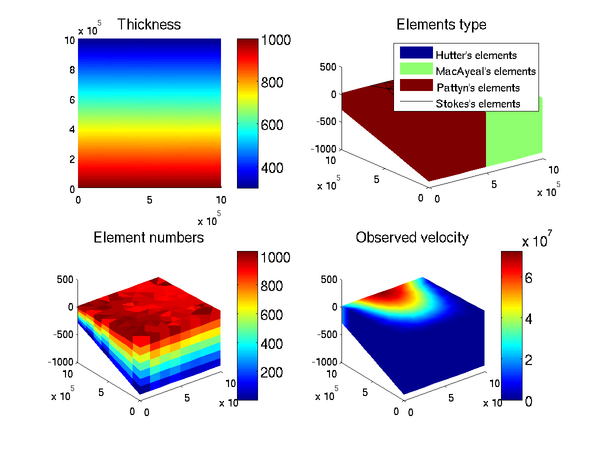
\includegraphics[width=\textwidth]{\assetsParentPath/assets/img/getting-started/plotting/matlab/plot.png}
	\end{center}
\end{figure}
This can work for any field of length \lstinlinebg|md.mesh.numberofelements| or \lstinlinebg|md.mesh.numberofvertices|.
%}}}
\subsubsection{Options}%{{{
Options in \lstinlinebg|plotmodel| come as pairs: the option name must be followed by its value. For example, if one wants to remove the color bar, the option name is \lstinlinebg|'colorbar'| and the value \lstinlinebg|0|:
\begin{lstlisting}
>> plotmodel(md, 'data', md.initialization.vel, 'colorbar', 0)
\end{lstlisting}
any options (except \lstinlinebg|'data'|) can be followed by \lstinlinebg|'#<i>'| where \lstinlinebg|<i>| is the subplot number, or \lstinlinebg|'#all'| if applied to all plots. For example:
\begin{lstlisting}
>> plotmodel(md, 'data', md.initialization.vel, 'data', 'mesh', 'view#2', 3, 'colorbar#all', 'on', 'axis#1', 'off equal')
\end{lstlisting}

\paragraph{axis}
Same as standard \href{http://www.mathworks.com/help/techdoc/ref/axis.html}{axis} MATLAB option:
\begin{lstlisting}
>> plotmodel(md, 'data', md.vel, 'axis', 'tight')
\end{lstlisting}

\paragraph{view}
Same as standard \href{http://www.mathworks.com/help/techdoc/ref/view.html}{view} MATLAB option:
\begin{lstlisting}
>> plotmodel(md, 'data', md.vel, 'view', 2)
\end{lstlisting}

\paragraph{xlim, ylim, zlim}
Same as standard \href{http://www.mathworks.com/help/techdoc/ref/xlim.html}{xlim} MATLAB option:
\begin{lstlisting}
>> plotmodel(md, 'data', md.vel, 'xlim', [10^5 2*10^5])
\end{lstlisting}

\paragraph{caxis}
Same as standard \href{http://www.mathworks.com/access/helpdesk/help/techdoc/index.html?/access/helpdesk/help/techdoc/ref/caxis.html}{caxis} MATLAB option (control the extreme values of the colorbar):
\begin{lstlisting}
>> plotmodel(md, 'data', md.vel, 'caxis', [0 1000])
\end{lstlisting}
\begin{figure}[H]
	\begin{center}
		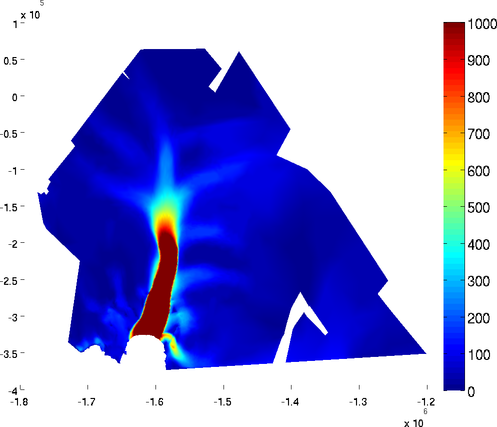
\includegraphics[width=\textwidth]{\assetsParentPath/assets/img/getting-started/plotting/matlab/caxis.png}
	\end{center}
\end{figure}

\paragraph{colorbar}
This option is used to control the colorbar display (\lstinlinebg|'on'| or \lstinlinebg|'off'|):
\begin{lstlisting}
>> plotmodel(md, 'data', md.vel, 'colorbar', 'off')
\end{lstlisting}

\paragraph{colormap}
Same as standard \href{http://www.mathworks.com/access/helpdesk/help/techdoc/index.html?/access/helpdesk/help/techdoc/ref/colormap.html}{colormap} MATLAB option (control the extreme values of the colorbar):
\begin{lstlisting}
>> plotmodel(md, 'data', md.vel, 'colormap', 'hsv')
\end{lstlisting}
\begin{figure}[H]
	\begin{center}
		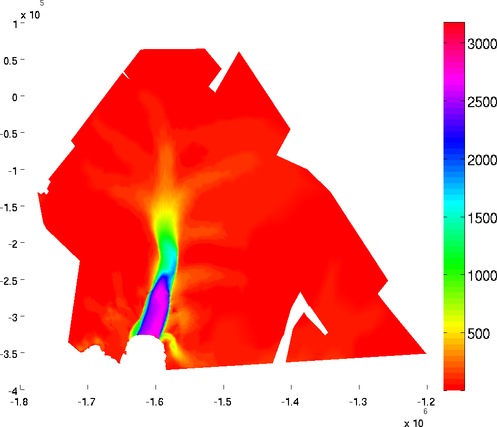
\includegraphics[width=\textwidth]{\assetsParentPath/assets/img/getting-started/plotting/matlab/colormap.png}
	\end{center}
\end{figure}

\paragraph{log}
To get a logarithmic colorbar, use the \lstinlinebg|'log'| option followed by \lstinlinebg|10| for a decimal logarithm:
\begin{lstlisting}
>> plotmodel(md, 'data', md.vel, 'log', 10)
\end{lstlisting}
\begin{figure}[H]
	\begin{center}
		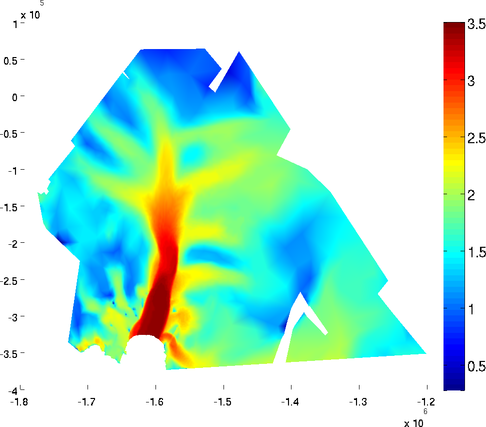
\includegraphics[width=\textwidth]{\assetsParentPath/assets/img/getting-started/plotting/matlab/log.png}
	\end{center}
\end{figure}

\paragraph{contourlevels}
Contours of equi-value can be added to the plot by using the \lstinlinebg|'contourlevels'| option. The number of contours can be chosen by using the \lstinlinebg|'contourlevels'| options. The user can specify a number of levels or a cell containing the values of color changes. For example:
\begin{lstlisting}
>> plotmodel(md, 'data', md.vel, 'contourlevels', 3)
\end{lstlisting}
\begin{figure}[H]
	\begin{center}
		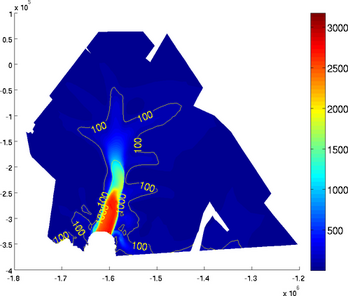
\includegraphics[width=\textwidth]{\assetsParentPath/assets/img/getting-started/plotting/matlab/contour3.png}
	\end{center}
\end{figure}
\begin{lstlisting}
>> plotmodel(md, 'data', md.vel, 'contourlevels', {100, 200, 500, 1000, 2000, 2500})
\end{lstlisting}
\begin{figure}[H]
	\begin{center}
		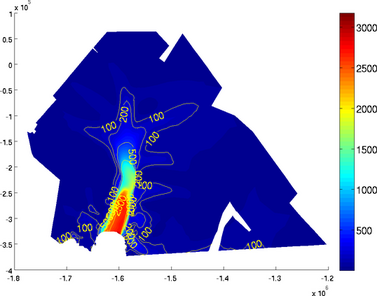
\includegraphics[width=\textwidth]{\assetsParentPath/assets/img/getting-started/plotting/matlab/contourcell.png}
	\end{center}
\end{figure}

\paragraph{contourticks}
If the user does not want to display the contour levels ticks, use the \lstinlinebg|'contourticks'| set as \lstinlinebg|'off'|:
\begin{lstlisting}
>> plotmodel(md, 'data', md.vel, 'contourlevels', {100, 200, 500, 1000, 2000, 2500}, 'contourticks', 'off')
\end{lstlisting}
\begin{figure}[H]
	\begin{center}
		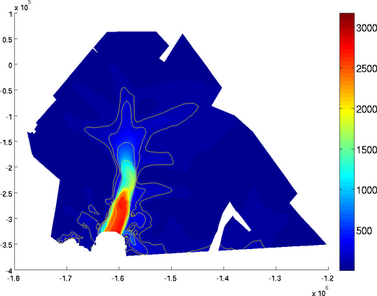
\includegraphics[width=\textwidth]{\assetsParentPath/assets/img/getting-started/plotting/matlab/contourticks.png}
	\end{center}
\end{figure}

\paragraph{contouronly}
If the user wants to display the contours only, use the \lstinlinebg|'contouronly'| set as \lstinlinebg|'on'|:
\begin{lstlisting}
>> plotmodel(md, 'data', 'vel', 'contourlevels', {100, 200, 500, 1000, 2000, 2500}, 'contouronly', 'on')
\end{lstlisting}

\paragraph{streamlines}
Streamlines can be displayed by using the \lstinlinebg|'streamlines'| option followed by a number of streamlines or a cell containing the coordinates of seed points:
\begin{lstlisting}
>> plotmodel(md, 'data', md.initialization.vel, 'streamlines', 50)
\end{lstlisting}
\begin{lstlisting}
>> plotmodel(md, 'data', md.initialization.vel, 'streamlines', {10^6 * [-1.45 -0.27], 10^6 * [-1.6 0]})
\end{lstlisting}
\begin{figure}[H]
	\begin{center}
		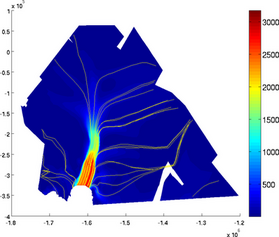
\includegraphics[width=0.475\textwidth]{\assetsParentPath/assets/img/getting-started/plotting/matlab/streamlines50.png}
		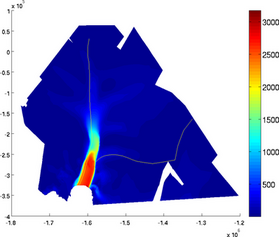
\includegraphics[width=0.475\textwidth]{\assetsParentPath/assets/img/getting-started/plotting/matlab/streamlinescell.png}
	\end{center}
\end{figure}

NOTE: Streamlines use the velocities that are in \lstinlinebg|md.initialization|. Make sure you transfer the calculated velocities to \lstinlinebg|md.initialization| if you want to display the calculated streamlines.

\paragraph{edgecolor}
The mesh can be superimposed onto the plot by using the \lstinlinebg|'edgecolor'| option followed by a color:
\begin{lstlisting}
>> plotmodel(md, 'data', md.initialization.vel, 'edgecolor', 'w')
\end{lstlisting}
\begin{figure}[H]
	\begin{center}
		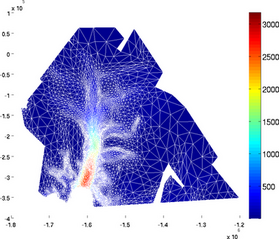
\includegraphics[width=\textwidth]{\assetsParentPath/assets/img/getting-started/plotting/matlab/edgecolor.png}
	\end{center}
\end{figure}

\paragraph{expdisp}
Any ARGUS file can be displayed with the \lstinlinebg|'expdisp'| option followed by the name of the ARGUS file:
\begin{lstlisting}
>> plotmodel(md, 'data', md.initialization.vel, 'expdisp', 'Iceshelves.exp')
\end{lstlisting}

\paragraph{expstyle}
The style of the ARGUS profile can be controlled with the \lstinlinebg|'expstyle'| option, followed by the desired line style. Here is an example for a yellow dotted line:
\begin{lstlisting}
>> plotmodel(md, 'data', md.initialization.vel, 'expdisp', 'Iceshelves.exp', 'expstyle', '--y')
\end{lstlisting}

\paragraph{mask}
If one does not want to display the value of the field on a mask only, use the \lstinlinebg|'mask'| option followed by a vector that holds 0 for the vertices whose values are hidden:
\begin{lstlisting}
>> plotmodel(md, 'data', md.initialization.vel, 'mask', md.mask.ocean_levelset < 0)
\end{lstlisting}
\begin{figure}[H]
	\begin{center}
		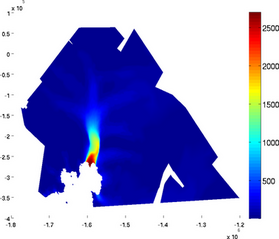
\includegraphics[width=\textwidth]{\assetsParentPath/assets/img/getting-started/plotting/matlab/mask.png}
	\end{center}
\end{figure}

\paragraph{northarrow}
An arrow pointing North can be added with the \lstinlinebg|'northarrow'| option followed by \lstinlinebg|'on'|. The shape and position of the arrow can be controlled by using \lstinlinebg|[x0 y0 length [ratio [width]]]| 
instead of \lstinlinebg|'on'|:
\begin{lstlisting}
>> plotmodel(md, 'data', md.initialization.vel, 'northarrow', 'on')
\end{lstlisting}

\paragraph{scaleruler}
A scale ruler can be added. As for the North arrow, the default display is done by \lstinlinebg|'on'| but the shape and position of the scale ruler can be controlled by \lstinlinebg|[x0 y0 length width numberofticks]| where (x0,y0) are the coordinates of the lower left corner:
\begin{lstlisting}
>> plotmodel(md, 'data', md.initialization.vel, 'scaleruler', 'on')
\end{lstlisting}

\paragraph{title}
Same as standard \href{http://www.mathworks.com/help/techdoc/ref/title.html}{title} MATLAB option:
\begin{lstlisting}
>> plotmodel(md, 'data', md.vel, 'title', 'Ice velocity [m/yr]')
\end{lstlisting}

\paragraph{fontsize}
Same as standard \href{http://www.mathworks.com/help/techdoc/ref/text_props.html}{fontsize} MATLAB option:
\begin{lstlisting}
>> plotmodel(md, 'data', md.vel, 'title', 'Ice velocity [m/yr]', 'fontsize', 8)
\end{lstlisting}

\paragraph{fontweight}
Same as standard \href{http://www.mathworks.com/help/techdoc/ref/text_props.html}{fontweight} MATLAB option:
\begin{lstlisting}
>> plotmodel(md, 'data', md.vel, 'title', 'Ice velocity [m/yr]', 'fontweight', 'b')
\end{lstlisting}

\paragraph{xlabel, ylabel}
Same as standard \href{http://www.mathworks.com/help/techdoc/ref/xlabel.html}{xlabel} MATLAB option:
\begin{lstlisting}
>> plotmodel(md, 'data', md.vel, 'xlabel', 'x axis [m]')
\end{lstlisting}
%}}}
\subsubsection{Special plots}%{{{
\paragraph{basaldrag}%{{{
The special plot \lstinlinebg|'basal_drag'| displays the norm of the basal drag friction in kPa following formula:
\begin{equation}
	\boldsymbol{\tau}_b = -k^2 N^r \|{\bf v}\|^{s-1} {\bf v}_b
\end{equation}
Basal drag relies on the velocity provided in \lstinlinebg|md.initialization|. The x and y components of the basal drag can be displayed with the \lstinlinebg|'basal_dragx'| or \lstinlinebg|'basal_dragy'| special plots:
\begin{lstlisting}
>> plotmodel(md, 'data', 'basal_drag')
\end{lstlisting}
\begin{lstlisting}
>> plotmodel(md, 'data', 'basal_dragx')
\end{lstlisting}
\begin{figure}[H]
	\begin{center}
		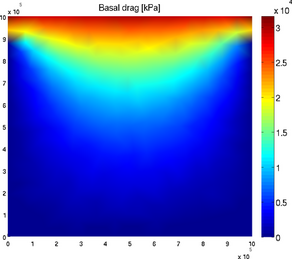
\includegraphics[width=0.475\textwidth]{\assetsParentPath/assets/img/getting-started/plotting/matlab/basaldrag.png}
		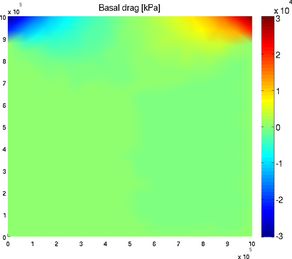
\includegraphics[width=0.475\textwidth]{\assetsParentPath/assets/img/getting-started/plotting/matlab/basaldragcomp.png}
		\caption{Basal friction norm and Basal friction x-component}
	\end{center}
\end{figure}
%}}}

\paragraph{BC}%{{{
The special plot \lstinlinebg|'BC'| displays all boundary conditions (Newmann and Dirichlet) for 2D and 3D meshes:
\begin{lstlisting}
>> plotmodel(md, 'data', 'BC')
\end{lstlisting}
\begin{figure}[H]
	\begin{center}
		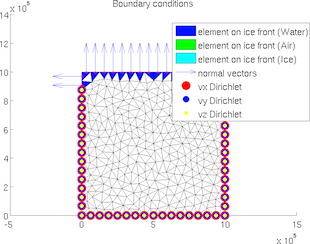
\includegraphics[width=\textwidth]{\assetsParentPath/assets/img/getting-started/plotting/matlab/BC.png}
	\end{center}
\end{figure}
%}}}
\paragraph{driving\_stress}%{{{
The special plot \lstinlinebg|'driving_stress'| displays the basal drag friction in kPa following formula:
\begin{equation}
	\boldsymbol{\tau}_d = \rho g H\;\nabla s
	\label{plotspecial_driving_stress}
\end{equation}
\begin{lstlisting}
>> plotmodel(md, 'data', 'driving_stress')
\end{lstlisting}
\begin{figure}[H]
	\begin{center}
		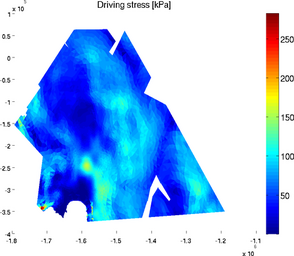
\includegraphics[width=\textwidth]{\assetsParentPath/assets/img/getting-started/plotting/matlab/driving_stress.png}
	\end{center}
\end{figure}
%}}}
\paragraph{elementnumbering}%{{{
In the debugging process, it is often very useful to display all the elements next to their numbers. This is what the special plot \lstinlinebg|'elementnumbering'| does:
\begin{lstlisting}
>> plotmodel(md, 'data', 'elementnumbering')
\end{lstlisting}
\begin{figure}[H]
	\begin{center}
		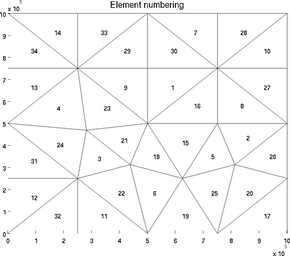
\includegraphics[width=\textwidth]{\assetsParentPath/assets/img/getting-started/plotting/matlab/elementnumbering.png}
	\end{center}
\end{figure}
A given list of elements can be highlighted with the \lstinlinebg|'highlight'| option:
\begin{lstlisting}
>> plotmodel(md, 'data', 'elementnumbering', 'highlight', [3 4 5 6 7])
\end{lstlisting}
\begin{figure}[H]
	\begin{center}
		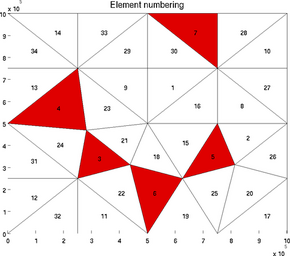
\includegraphics[width=\textwidth]{\assetsParentPath/assets/img/getting-started/plotting/matlab/elementnumbering_highlight.png}
	\end{center}
\end{figure}
%}}}
\paragraph{elements\_type}%{{{
The special plot \lstinlinebg|'elements_type'| displays the elements with a specific color for each formulation:
\begin{lstlisting}
>> plotmodel(md, 'data', 'elements_type')
\end{lstlisting}
\begin{figure}[H]
	\begin{center}
		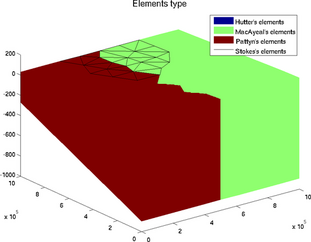
\includegraphics[width=\textwidth]{\assetsParentPath/assets/img/getting-started/plotting/matlab/elements_type.png}
	\end{center}
\end{figure}
%}}}
\paragraph{vertexnumbering}%{{{
In the debugging process, it is often very useful to display all the vertices next to their numbers. This is what the special plot \lstinlinebg|'vertexnumbering'| does:
\begin{lstlisting}
>> plotmodel(md, 'data', 'vertexnumbering')
\end{lstlisting}
\begin{figure}[H]
	\begin{center}
		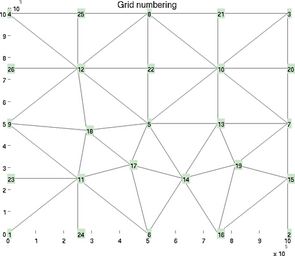
\includegraphics[width=\textwidth]{\assetsParentPath/assets/img/getting-started/plotting/matlab/gridnumbering.png}
	\end{center}
\end{figure}

A given list of vertices can be highlighted with the \lstinlinebg|'highlight'| option:
\begin{lstlisting}
>> plotmodel(md, 'data', 'vertexnumbering', 'highlight', [2 5 7 12])
\end{lstlisting}
\begin{figure}[H]
	\begin{center}
		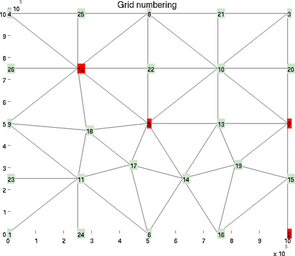
\includegraphics[width=\textwidth]{\assetsParentPath/assets/img/getting-started/plotting/matlab/gridnumbering_highlight.png}
	\end{center}
\end{figure}
%}}}
\paragraph{highlightelements}%{{{
The special plot \lstinlinebg|'highlightelements'| is very similar to the plot \lstinlinebg|'elementnumbering'|. It is another possibility to highlight one or several grids, but without indicating the number of all the elements. It is a lot faster for large models:
\begin{lstlisting}
>> plotmodel(md, 'data', 'highlightelements', 'highlight', 5)
\end{lstlisting}
\begin{lstlisting}
>> plotmodel(md, 'data', 'highlightelements', 'highlight', [5 12])
\end{lstlisting}
\begin{figure}[H]
	\begin{center}
		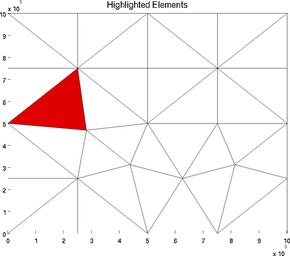
\includegraphics[width=0.475\textwidth]{\assetsParentPath/assets/img/getting-started/plotting/matlab/highlightelements_highlight.png}
		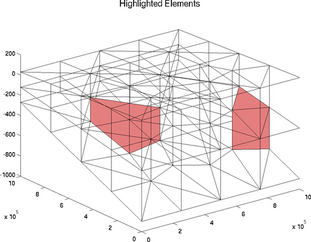
\includegraphics[width=0.475\textwidth]{\assetsParentPath/assets/img/getting-started/plotting/matlab/highlightelements_highlight3d.png}
	\end{center}
\end{figure}
%}}}
\paragraph{highlightgrids}%{{{
The special plot \lstinlinebg|'highlightgrids'| is very similar to \lstinlinebg|'gridnumbering'|. It is another possibility to highlight grids without indicating all the grids numbers. It is a lot faster for big models:
\begin{lstlisting}
>> plotmodel(md, 'data', 'highlightgrids', 'highlight', [12 20])
\end{lstlisting}
\begin{lstlisting}
>> plotmodel(md, 'data', 'highlightgrids', 'highlight', [12 16 26])
\end{lstlisting}
\begin{figure}[H]
	\begin{center}
		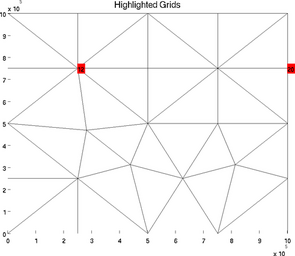
\includegraphics[width=0.475\textwidth]{\assetsParentPath/assets/img/getting-started/plotting/matlab/highlightgrids_highlight.png}
		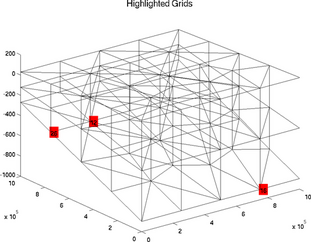
\includegraphics[width=0.475\textwidth]{\assetsParentPath/assets/img/getting-started/plotting/matlab/highlightgrids_highlight3d.png}
	\end{center}
\end{figure}
%}}}
\paragraph{icefront}%{{{
The special plot \lstinlinebg|'icefront'| displays the Neumann boundary conditions, i.e. all the segments on ice front and the normal to these segments, for a 2D or 3D mesh:
\begin{lstlisting}
>> plotmodel(md, 'data', 'icefront')
\end{lstlisting}
\begin{figure}[H]
	\begin{center}
		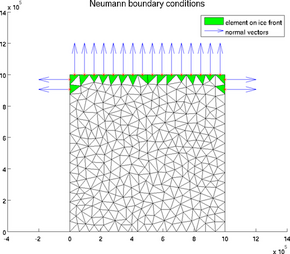
\includegraphics[width=0.475\textwidth]{\assetsParentPath/assets/img/getting-started/plotting/matlab/icefront2d.png}
		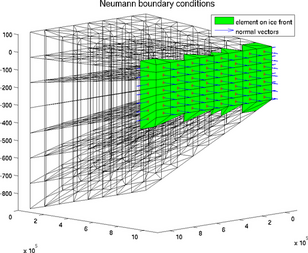
\includegraphics[width=0.475\textwidth]{\assetsParentPath/assets/img/getting-started/plotting/matlab/icefront3d.png}
	\end{center}
\end{figure}
%}}}
\paragraph{mesh}%{{{
The special plot \lstinlinebg|'mesh'| displays the mesh of 2D or 3D model:
\begin{lstlisting}
>> plotmodel(md, 'data', 'mesh')
\end{lstlisting}
\begin{figure}[H]
	\begin{center}
		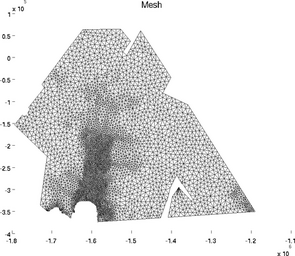
\includegraphics[width=0.475\textwidth]{\assetsParentPath/assets/img/getting-started/plotting/matlab/mesh2d.png}
		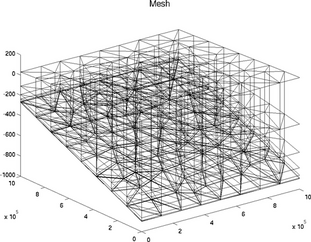
\includegraphics[width=0.475\textwidth]{\assetsParentPath/assets/img/getting-started/plotting/matlab/mesh3d.png}
	\end{center}
\end{figure}
%}}}
%}}}
\subsubsection{Quiver plot}%{{{
For 2D or 3D fields, a generic color plot cannot be used (except component by component). The \lstinlinebg|'data'| used by the function \lstinlinebg|plotmodel| must be a matrix of 2 or 3 columns. For example:
\begin{lstlisting}
>> plotmodel(md, 'data', [md.vx md.vy])
\end{lstlisting}
\begin{figure}[H]
	\begin{center}
		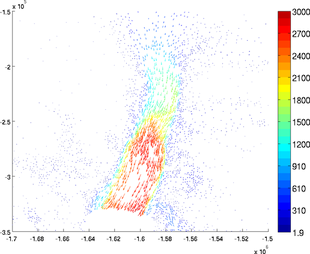
\includegraphics[width=\textwidth]{\assetsParentPath/assets/img/getting-started/plotting/matlab/plotquiver.png}
	\end{center}
\end{figure}

\paragraph{ColorLevels}
The number of colors can be chosen by using the \lstinlinebg|'colorlevels'| options. The user can specify a number of levels or a cell containing the values of color changes. For example:
\begin{lstlisting}
>> plotmodel(md, 'data', [md.vx md.vy], 'colorlevels', 3)
\end{lstlisting}
\begin{lstlisting}
>> plotmodel(md, 'data', [md.vx md.vy], 'colorlevels', 100)
\end{lstlisting}
\begin{figure}[H]
	\begin{center}
		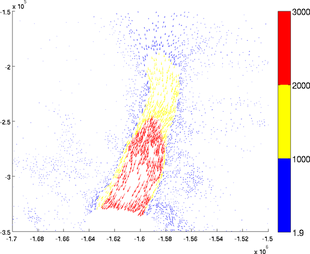
\includegraphics[width=0.475\textwidth]{\assetsParentPath/assets/img/getting-started/plotting/matlab/color3.png}
		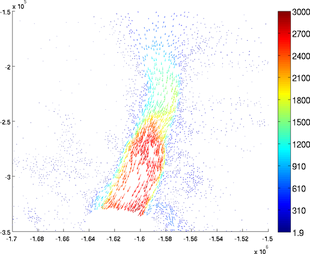
\includegraphics[width=0.475\textwidth]{\assetsParentPath/assets/img/getting-started/plotting/matlab/color100.png}
	\end{center}
\end{figure}
\begin{lstlisting}
>> plotmodel(md, 'data', [md.vx md.vy], 'colorlevels', {100, 200, 500, 1000, 2000, 2500})
\end{lstlisting}
\begin{figure}[H]
	\begin{center}
		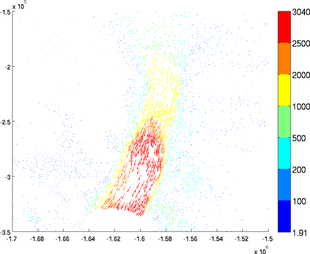
\includegraphics[width=\textwidth]{\assetsParentPath/assets/img/getting-started/plotting/matlab/colorcell.png}
	\end{center}
\end{figure}

\paragraph{Scaling}
The arrows length can be modified with the \lstinlinebg|'scaling'| options. The default value is 0.4. A higher scaling value will result in longer arrows:
\begin{lstlisting}
>> plotmodel(md, 'data', [md.vx md.vy], 'scaling', 1)
\end{lstlisting}
\begin{lstlisting}
>> plotmodel(md, 'data', [md.vx md.vy], 'scaling', 0.1)
\end{lstlisting}
\begin{figure}[H]
	\begin{center}
		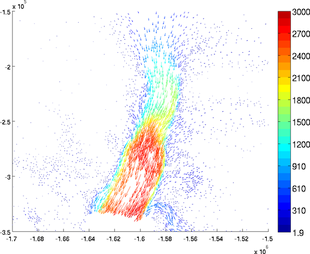
\includegraphics[width=0.475\textwidth]{\assetsParentPath/assets/img/getting-started/plotting/matlab/scaling1.png}
		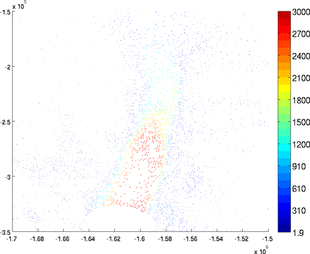
\includegraphics[width=0.475\textwidth]{\assetsParentPath/assets/img/getting-started/plotting/matlab/scaling01.png}
	\end{center}
\end{figure}

\paragraph{Autoscale}
If the user wants all the arrows to have the same length, use the option \lstinlinebg|'autoscale'| set as \lstinlinebg|'off'|:
\begin{lstlisting}
>> plotmodel(md, 'data', [md.vx md.vy], 'autoscale', 'off')
\end{lstlisting}
\begin{figure}[H]
	\begin{center}
		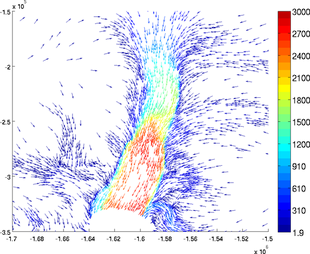
\includegraphics[width=\textwidth]{\assetsParentPath/assets/img/getting-started/plotting/matlab/autoscale.png}
	\end{center}
\end{figure}

\paragraph{Density}
The number of arrows can be reduced with the option \lstinlinebg|'density'|. If the density is set as 3, only one arrow out of 3 will be displayed. This option is very useful when the mesh is very refined:
\begin{lstlisting}
>> plotmodel(md, 'data', [md.vx md.vy], 'density', 3)
\end{lstlisting}
\begin{figure}[H]
	\begin{center}
		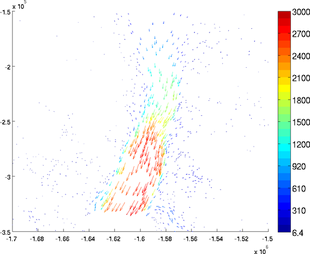
\includegraphics[width=\textwidth]{\assetsParentPath/assets/img/getting-started/plotting/matlab/density3.png}
	\end{center}
\end{figure}
%}}}
\subsubsection{Cross section}%{{{
The section plot can be used to display the value of a field on a given track. The option \lstinlinebg|'sectionvalue'| must be followed by the name of an ARGUS file which contained the coordinates of the points describing the profile (this file can be generated by \lstinlinebg|exptool.m|). The resulting plot will be a curve in 2D and a colored surface in 3D. For example:
\begin{lstlisting}
>> plotmodel(md, 'data', md.vel, 'expdisp', 'track.exp')
\end{lstlisting}
\begin{figure}[H]
	\begin{center}
		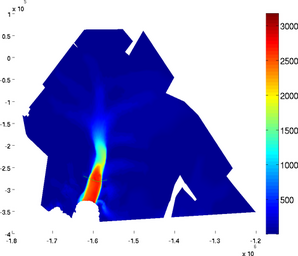
\includegraphics[width=\textwidth]{\assetsParentPath/assets/img/getting-started/plotting/matlab/track.png}
	\end{center}
\end{figure}
\begin{lstlisting}
>> plotmodel(md, 'data', md.vel, 'sectionvalue', 'track.exp')
\end{lstlisting}
\begin{figure}[H]
	\begin{center}
		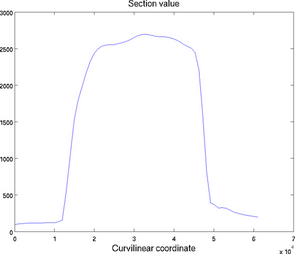
\includegraphics[width=0.475\textwidth]{\assetsParentPath/assets/img/getting-started/plotting/matlab/2d.png}
		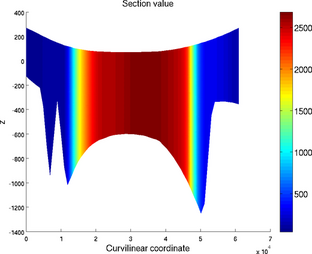
\includegraphics[width=0.475\textwidth]{\assetsParentPath/assets/img/getting-started/plotting/matlab/3d.png}
		\caption{Section plot for 2D (left) and 3D (right) models}
	\end{center}
\end{figure}

\paragraph{Resolution}
The horizontal and vertical (in 3D) resolution can be specified by the \lstinlinebg|'resolution'| option. It must be a list with the horizontal resolution followed by the vertical resolution (in meters). When not specified, the default resolution is displayed:
\begin{lstlisting}
>> plotmodel(md, 'data', md.vel, 'sectionvalue', 'track.exp', 'resolution', [2*10^4 0])
\end{lstlisting}
\begin{lstlisting}
>> plotmodel(md, 'data', md.vel, 'sectionvalue', 'track.exp', 'resolution', [10^3 0])
\end{lstlisting}

\paragraph{Show section}
The profile used to create the section plot can be also plotted with the \lstinlinebg|'showsection'| option:
\begin{lstlisting}
>> plotmodel(md, 'data', md.vel, 'showsection', 'on')
\end{lstlisting}
\begin{figure}[H]
	\begin{center}
		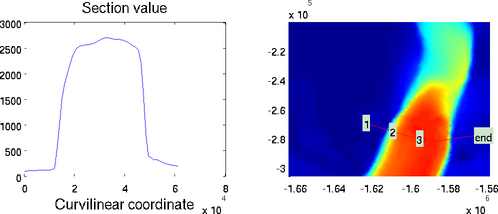
\includegraphics[width=\textwidth]{\assetsParentPath/assets/img/getting-started/plotting/matlab/show.png}
	\end{center}
\end{figure}
%}}}

\clearpage % Make sure all figures are placed before next section

% Just The Docs Front Matter
% title: Plotting in Python
% parent: Plotting
% nav_order: 2
% has_children: false
% has_toc: false

\subsection{Plotting in Python} \label{sec:getting-started-plotting-python}
We are currently working on a standard API for plotting ISSM results in a Python interface.

\clearpage % Make sure all figures are placed before next section


%%%%%%%%%%%%%%%%%%%%%%%%%%%%%%%%%%%%%%%%%%%%%%%%%%%%%%%%%%%%%%%%%%%%%%%%%%%%%%%%

\chapter{Using ISSM} \label{chap:using-issm}
% Just The Docs Front Matter
% title: Using ISSM
% nav_order: 4
% has_children: true
% has_toc: false

%__@LATEX_ONLY_START@__
\section{Introduction} \label{sec:using-issm}
%__@LATEX_ONLY_END@__or for development is covered in the
%__@MARKDOWN_ONLY_START@__
%<h1>Using ISSM</h1>
%__@MARKDOWN_ONLY_END@__

%__@LATEX_ONLY_START@__
\begin{itemize}
	\item \hyperref[sec:using-issm-tutorials]{Tutorials}
	\item \hyperref[sec:using-issm-capabilities]{Capabilities}
	\item \hyperref[sec:using-issm-parameterization]{Parameterization}
	\item \hyperref[sec:using-issm-advanced]{Advanced}
\end{itemize}
%__@LATEX_ONLY_END@__
%__@MARKDOWN_ONLY_START@__
%- <a href="tutorials" target="_top">Tutorials</a>
%- <a href="capabilities" target="_top">Capabilities</a>
%- <a href="parameterization" target="_top">Parameterization</a>
%- <a href="advanced" target="_top">Advanced</a>
%__@MARKDOWN_ONLY_END@__

\subsection{Introduction to Capabilities Video Series}
Dr. Eric Larour and members of the ISSM development team have developed a series of videos to introduce viewers to practical uses of a number of ISSM's capabilities.

%__@MARKDOWN_ONLY_START@__
%<iframe width="560" height="315" src="https://www.youtube-nocookie.com/embed/a7WorVjnYZc?si=n-y59DueCo-btINT" title="YouTube video player" frameborder="0" allow="accelerometer; autoplay; clipboard-write; encrypted-media; gyroscope; picture-in-picture; web-share" referrerpolicy="strict-origin-when-cross-origin" allowfullscreen></iframe>
%
%<iframe width="560" height="315" src="https://www.youtube-nocookie.com/embed/2kTncXsoGPQ?si=6kO9WXwd7hLlK8xI" title="YouTube video player" frameborder="0" allow="accelerometer; autoplay; clipboard-write; encrypted-media; gyroscope; picture-in-picture; web-share" referrerpolicy="strict-origin-when-cross-origin" allowfullscreen></iframe>
%
%<iframe width="560" height="315" src="https://www.youtube-nocookie.com/embed/0g1atAnw104?si=HagF4fL0AGMOZhmH" title="YouTube video player" frameborder="0" allow="accelerometer; autoplay; clipboard-write; encrypted-media; gyroscope; picture-in-picture; web-share" referrerpolicy="strict-origin-when-cross-origin" allowfullscreen></iframe>
%
%<iframe width="560" height="315" src="https://www.youtube-nocookie.com/embed/KtpBtioOW1E?si=olFoDYUFax2SW65r" title="YouTube video player" frameborder="0" allow="accelerometer; autoplay; clipboard-write; encrypted-media; gyroscope; picture-in-picture; web-share" referrerpolicy="strict-origin-when-cross-origin" allowfullscreen></iframe>
%
%<iframe width="560" height="315" src="https://www.youtube-nocookie.com/embed/iFHdMozWzm0?si=DRE2crkk4bDTNTVw" title="YouTube video player" frameborder="0" allow="accelerometer; autoplay; clipboard-write; encrypted-media; gyroscope; picture-in-picture; web-share" referrerpolicy="strict-origin-when-cross-origin" allowfullscreen></iframe>
%__@MARKDOWN_ONLY_END@__

%__@LATEX_ONLY_START@__
\begin{itemize}
	\item \href{https://youtu.be/a7WorVjnYZc}{ISSM Tutorial 1}
	\item \href{https://youtu.be/2kTncXsoGPQ}{ISSM Tutorial 2}
	\item \href{https://youtu.be/0g1atAnw104}{ISSM Tutorial 3}
	\item \href{https://youtu.be/KtpBtioOW1E}{ISSM Tutorial 4}
	\item \href{https://youtu.be/iFHdMozWzm0}{ISSM Tutorial 5}
\end{itemize}
%__@LATEX_ONLY_END@__

\clearpage % Make sure all figures are placed before next section


%\section{Tutorials}
% Just The Docs Front Matter
% title: Tutorials
% layout: default
% parent: Using ISSM
% nav_order: 1
% has_children: true
% has_toc: false

\section{Tutorials} \label{sec:using-issm-tutorials}
In order to run the tutorials, you need to download some 
%__@LATEX_ONLY_START@__
\hyperref[sec:using-issm-tutorials-datasets]{Datasets}
%__@LATEX_ONLY_END@__
%__@MARKDOWN_ONLY_START@__
% <a href="datasets">datasets</a>.
%__@MARKDOWN_ONLY_END@__

%__@LATEX_ONLY_START@__
\begin{itemize}
	\item \hyperref[sec:using-issm-tutorials-squareiceshelf]{Square Ice Shelf}
	\item \hyperref[sec:using-issm-tutorials-mesh]{Mesh Adaptation}
	\item \hyperref[sec:using-issm-tutorials-iceflowmodels]{Ice Flow Models (under development)}
	\item \hyperref[sec:using-issm-tutorials-ismip]{Ice Sheet Model Intercomparison Project (ISMIP) Tests}
	\item \hyperref[sec:using-issm-tutorials-inversions]{Inversions}
	\item \hyperref[sec:using-issm-tutorials-greenland]{Modeling the Greenland Ice Sheet (SeaRISE)}
	\item \hyperref[sec:using-issm-tutorials-icebridge]{Modeling the Greenland Ice Sheet Using IceBridge Data}
	\item \hyperref[sec:using-issm-tutorials-pig]{Modeling Pine Island Glacier}
	\item \hyperref[sec:using-issm-tutorials-pigsensitivity]{Pine Island Glacier Sensitivity Study}
	\item \hyperref[sec:using-issm-tutorials-uncertaintyquantification]{Pine Island Glacier Uncertainty Quantification (requires Dakota)}
	\item \hyperref[sec:using-issm-tutorials-pigstissm]{Pine Island Glacier Stochastic Forcing (StISSM)}
	\item \hyperref[sec:using-issm-tutorials-jks]{Modeling Jakobshavn Isbr\ae}
	\item \hyperref[sec:using-issm-tutorials-shakti]{Subglacial Channel Formation From a Single Moulin (SHAKTI)}
	\item \hyperref[sec:using-issm-tutorials-helheim]{Modeling Helheim Glacier}
	\item \hyperref[sec:using-issm-tutorials-helheimshakti]{Subglacial Hydrology of Helheim Glacier (SHAKTI)}
	\item \hyperref[sec:using-issm-tutorials-amr]{Adaptive Mesh Refinement (AMR)}
	\item \hyperref[sec:using-issm-tutorials-sealevelfingerprints]{Sea-Level Fingerprints (GRACE)}
\end{itemize}
%__@LATEX_ONLY_END@__
%__@MARKDOWN_ONLY_START@__
% - <a href="squareiceshelf">Square Ice Shelf</a>
% - <a href="mesh">Mesh Adaptation</a>
% - <a href="iceflowmodels">Ice Flow Models (under development)</a>
% - <a href="ismip">Ice Sheet Model Intercomparison Project (ISMIP) Tests</a>
% - <a href="inversions">Inversions</a>
% - <a href="greenland">Modeling the Greenland Ice Sheet (SeaRISE)</a>
% - <a href="icebridge">Modeling the Greenland Ice Sheet Using IceBridge Data</a>
% - <a href="pig">Modeling Pine Island Glacier</a>
% - <a href="pigsensitivity">Pine Island Glacier Sensitivity Study</a>
% - <a href="uncertaintyquantification">Pine Island Glacier Uncertainty Quantification (requires Dakota)</a>
% - <a href="pigstissm">Pine Island Glacier Stochastic Forcing (StISSM)</a>
% - <a href="jks">Modeling Jakobshavn Isbr&aelig;</a>
% - <a href="shakti">Subglacial Channel Formation From a Single Moulin (SHAKTI)</a>
% - <a href="helheim">Modeling Helheim Glacier</a>
% - <a href="helheimshakti">Subglacial Hydrology of Helheim Glacier (SHAKTI)</a>
% - <a href="amr">Adaptive Mesh Refinement (AMR)</a>
% - <a href="sealevelfingerprints">Sea-Level Fingerprints (GRACE)</a>
%__@MARKDOWN_ONLY_END@__

\clearpage % Make sure all figures are placed before next section

% Just The Docs Front Matter
% title: Datasets
% parent: Tutorials
% has_children: false
% has_toc: false

\subsection{Datasets} \label{sec:using-issm-tutorials-datasets}
To run the tutorials, you will need to download a number of datasets. The easiest way to do this is to run,
\begin{lstlisting}
${ISSM_DIR}/scripts/DownloadExamplesDatasets.sh
\end{lstlisting}
The default behavior of this script is to download the datasets to the \lstinlinebg|../examples/Data| relative to the location of the script. If you wish to download them to another location, supply the optional path argument.

If you would prefer to download the datasets manually, use the following links, downloading each file to \lstinlinebg|${ISSM_DIR}/examples/Data|,
% NOTE: Do not remove the following: it allows us to target dataset links with 
%		the download script located in the ISSM code repository at 
%		examples/Data/DownloadExamplesDatasets.sh
%
%__@MARKDOWN_ONLY_START@__
%<!--DATASETS LIST START-->
%__@MARKDOWN_ONLY_END@__
\begin{itemize}
	\item \href{https://issm.jpl.nasa.gov/files/workshop2014/SquareShelf.nc}{Square ice shelf dataset}
	\item \href{https://issm.jpl.nasa.gov/files/examples/Antarctica_5km_withshelves_v0.75.nc}{SeaRISE Antarctica v0.75}
	\item \href{https://issm.jpl.nasa.gov/files/examples/Greenland_5km_dev1.2.nc}{SeaRISE Greenland dev1.2}
	\item \href{https://issm.ess.uci.edu/files/tutorials/Antarctica_ice_velocity.nc}{MEaSUREs Antarctic velocities}
	\item \href{https://issm.jpl.nasa.gov/files/workshop2014/CrossOvers2009.mat}{Pine Island ice thickness cross overs (Dakota)}
	\item \href{https://issm.jpl.nasa.gov/files/examples/Box_Greenland_SMB_monthly_1840-2012_5km_cal_ver20141007.nc}{Jason Box's SMB data}
	\item \href{https://data.cresis.ku.edu/data/grids/old_versions/Jakobshavn_2008_2011_Composite.zip}{Jakobshavn Isbr\ae\ bed map} \newline(we only need \lstinlinebg|grids/Jakobshavn_2008_2011_Composite_XYZGrid.txt|)
	\item \href{https://issm.jpl.nasa.gov/files/examples/GRACE_and_suporting_datasets.zip}{GRACE and supporting datasets for SESAW tutorials}
\end{itemize}
% NOTE: Do not remove the following: it allows us to target dataset links with 
%		the download script located in the ISSM code repository at 
%		examples/Data/DownloadExamplesDatasets.sh
%
%__@MARKDOWN_ONLY_START@__
%<!--DATASETS LIST END-->
%__@MARKDOWN_ONLY_END@__

\clearpage % Make sure all figures are placed before next section

% Just The Docs Front Matter
% title: Square Ice Shelf
% parent: Tutorials
% has_children: false
% has_toc: false

\subsection{Square Ice Shelf} \label{sec:using-issm-tutorials-squareiceshelf}
This is an example of velocity computation in steady state for a square ice shelf. First, launch MATLAB. In the left sidebar, select \lstinlinebg|ISSM_DIR| (the directory in which ISSM is stored) as your Current Directory. Then, navigate to \lstinlinebg|examples/SquareIceshelf|, which you can also do via the left sidebar or by running the following in the MATLAB Command Window:
\begin{lstlisting}
>> cd examples/SquareIceShelf
\end{lstlisting}

You can create an empty model structure by running:
\begin{lstlisting}
>> md = model;
\end{lstlisting}

Create a mesh of the domain outline with a resolution of 50,000 meters:
\begin{lstlisting}
>> md = triangle(md, 'DomainOutline.exp', 50000);
\end{lstlisting}

Define the glacier system as an ice shelf (no island):
\begin{lstlisting}
>> md = setmask(md, 'all', '');
\end{lstlisting}

Parameterize the model with the file \lstinlinebg|Square.par| (which you can see exists in the current directory by inspecting the left sidebar):
\begin{lstlisting}
>> md = parameterize(md, 'Square.par');
\end{lstlisting}

Define all elements as SSA:
\begin{lstlisting}
>> md = setflowequation(md, 'SSA', 'all');
\end{lstlisting}

Compute the velocity field of the ice shelf:
\begin{lstlisting}
>> md = solve(md, 'Stressbalance');
\end{lstlisting}

Finally, generate a plot of the velocity:
\begin{lstlisting}
>> plotmodel(md, 'data', md.results.StressbalanceSolution.Vel);
\end{lstlisting}

\begin{figure}[H]
	\begin{center}
		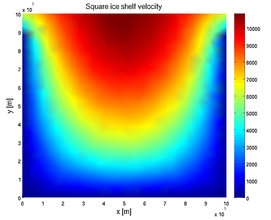
\includegraphics[width=\textwidth]{\assetsParentPath/assets/img/using-issm/tutorials/squareiceshelf/squarevel.png}
	\end{center}
\end{figure}

\clearpage % Make sure all figures are placed before next section

% Just The Docs Front Matter
% title: Mesh Adaptation
% parent: Tutorials
% has_children: false
% has_toc: false

\subsection{Mesh Adaptation} \label{sec:using-issm-tutorials-mesh}
\subsubsection{Goals} %{{{
In this tutorial, we show how to use the different meshers of ISSM:
\begin{itemize}
	\item Learn how to use the different meshers of ISSM:
		\begin{itemize}
			\item \lstinlinebg|squaremesh| for square domains (ISMIP)
			\item \lstinlinebg|roundmesh| for round domain (EISMINT)
			\item \lstinlinebg|triangle| (from J. Shewchuk)
			\item \lstinlinebg|bamg| (adapted from F. Hecht)
		\end{itemize}
	\item Use anisotropic mesh adaptation to optimize the mesh resolution spatially
\end{itemize}
Go to \lstinlinebg|<ISSM_DIR>/examples/Mesh/| to do this tutorial.
%}}}

\subsubsection{Squaremesh}%{{{
\lstinlinebg|squaremesh| generates structured uniform meshes for rectangular domains.
\paragraph{Usage}%{{{
\begin{lstlisting}
>> md = model;
>> md = squaremesh(md, 100, 200, 15, 25);
\end{lstlisting}
\lstinlinebg|squaremesh| takes the following arguments:
\begin{enumerate}
	\item model
	\item x-length (meters)
	\item y-length (meters)
	\item number of nodes along the x axis
	\item number of nodes along the y axis
\end{enumerate}
%}}}

\paragraph{Example}%{{{
The previous command creates the mesh shown below:
\begin{lstlisting}
>> plotmodel(md, 'data', 'mesh');
\end{lstlisting}
\begin{figure}[H]
	\begin{center}
		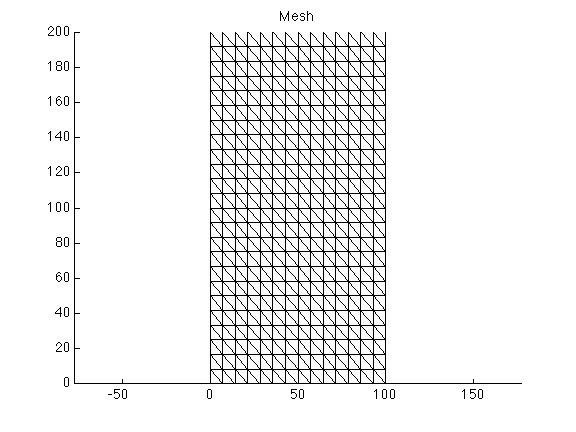
\includegraphics[width=\textwidth]{\assetsParentPath/assets/img/using-issm/tutorials/mesh/mesh1.png}
	\end{center}
\end{figure}
%}}}
%}}}
\subsubsection{Roundmesh}%{{{
\lstinlinebg|roundmesh| generates unstructured uniform meshes for circular domains.

\paragraph{Usage}%{{{
\begin{lstlisting}
>> md = roundmesh(model, 100, 10);
\end{lstlisting}
\lstinlinebg|roundmesh| takes the following arguments:
\begin{enumerate}
	\item model
	\item radius (meters)
	\item element size (meters)
\end{enumerate}
%}}}

\paragraph{Example}%{{{
The previous command creates the mesh shown below:
\begin{lstlisting}
>> plotmodel(md, 'data', 'mesh');
\end{lstlisting}
\begin{figure}[H]
	\begin{center}
		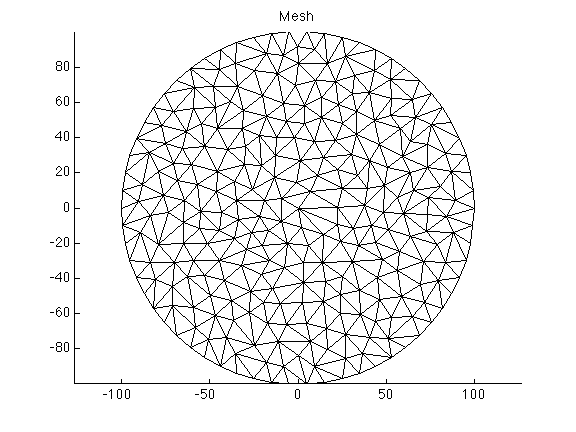
\includegraphics[width=\textwidth]{\assetsParentPath/assets/img/using-issm/tutorials/mesh/mesh2.png}
	\end{center}
\end{figure}
%}}}

\subsubsection{Triangle}%{{{
\lstinlinebg|triangle| is a very fast algorithm for mesh generation. Developed by \href{http://www.cs.cmu.edu/~quake/triangle.html}{J Shewchuk}, it generates unstructured triangular meshes.

\paragraph{Usage}%{{{
\begin{lstlisting}
>> md = triangle(model, 'Square.exp', .2);
\end{lstlisting}
\lstinlinebg|triangle| takes the following arguments:
\begin{enumerate}
	\item model
	\item ARGUS file of the domain outline (\lstinlinebg|.exp| extension, see the 
	%__@LATEX_ONLY_START@__
	\hyperref[sec:using-issm-capabilities-mesh-generation]{`Capabilities' $\rightarrow$ `Mesh Generation' section}
	%__@LATEX_ONLY_END@__
	%__@MARKDOWN_ONLY_START@__
	%<a href="../capabilities/mesh-generation" target="_top">'Capabilities' &#8594; 'Mesh Generation' page</a>
	%__@MARKDOWN_ONLY_END@__
	for more details)
	\item average element size (meters)
\end{enumerate}
The previous command creates the following mesh:
\begin{lstlisting}
>> plotmodel(md, 'data', 'mesh');
\end{lstlisting}
\begin{figure}[H]
	\begin{center}
		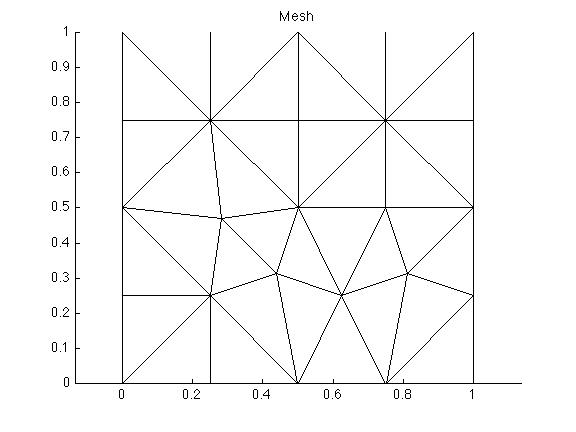
\includegraphics[width=\textwidth]{\assetsParentPath/assets/img/using-issm/tutorials/mesh/mesh3.png}
	\end{center}
\end{figure}
You can change the resolution from \lstinlinebg|0.2| to \lstinlinebg|0.05| to get a higher resolution.
%}}}

\subsubsection{Bamg}%{{{
BAMG stands for Bidimensional Anisotropic Mesh Generator. It was released in 2006 after more than 10 years of development by Frederic Hecht. It is now part of \href{http://www.freefem.org/ff++/}{FreeFEM++}. The algorithm that is available in ISSM is inspired by this software, but has been rewritten entirely.
%}}}

\paragraph{Usage}%{{{
\begin{lstlisting}
>> md = bamg(model, ...);
\end{lstlisting}
\lstinlinebg|bamg| takes as it's first argument a model, and then pairs of options
\begin{enumerate}
	\item model
	\item pairs of options (type \lstinlinebg|help bamg| to get a full list of options)
\end{enumerate}
%}}}

\paragraph{Uniform mesh}%{{{
To create a non-uniform mesh, use the following options:
\begin{enumerate}
	\item \lstinlinebg|'domain'| followed by the domain name
	\item \lstinlinebg|'hmax'| followed by the size (meters) of each triangle
\end{enumerate}
\begin{lstlisting}
>> md = bamg(model, 'domain', 'Square.exp', 'hmax', .05);
\end{lstlisting}
The previous command will create the following mesh (use \lstinlinebg|plotmodel(md, 'data', 'mesh')| to visualize the mesh):
\begin{figure}[H]
	\begin{center}
		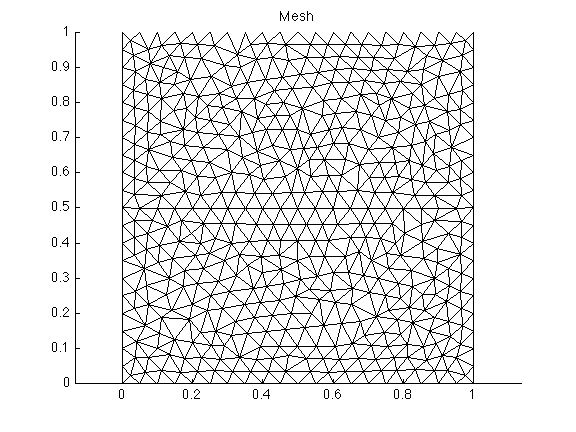
\includegraphics[width=\textwidth]{\assetsParentPath/assets/img/using-issm/tutorials/mesh/mesh4.png}
	\end{center}
\end{figure}
Note that the nodes are not as randomly distributed as \lstinlinebg|triangle|. The strength of BAMG is not for uniform meshes but for automatic mesh adaptation based on a metric.
%}}}

\paragraph{Non-Uniform mesh}%{{{
To create a non-uniform mesh, use the following options:
\begin{enumerate}
	\item \lstinlinebg|'domain'| followed by the domain name
	\item \lstinlinebg|'hvertices'| followed by the element size for each vertex of the domain outline
\end{enumerate}
In our example, \lstinlinebg|Square.exp| has 4 vertices. If we want a resolution of 0.2, except in the vicinity of the third node, we use the following commands:
\begin{lstlisting}
>> md = model;
>> hvertices = [0.2; 0.2; 0.005; 0.2];
>> md = bamg(md, 'domain', 'Square.exp', 'hvertices', hvertices);
\end{lstlisting}
Use the \lstinlinebg|plotmodel(md, 'data', 'mesh')| command to visualize the newly defined mesh:
\begin{figure}[H]
	\begin{center}
		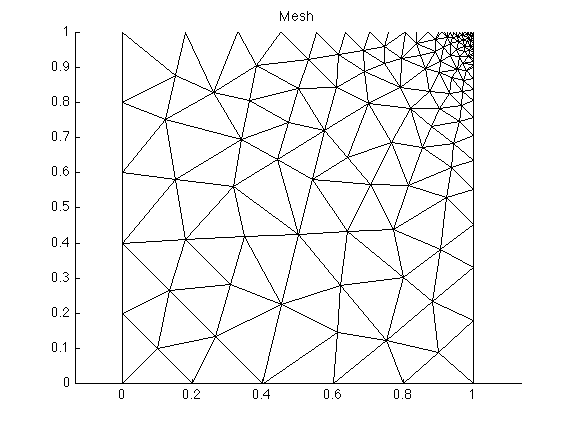
\includegraphics[width=\textwidth]{\assetsParentPath/assets/img/using-issm/tutorials/mesh/mesh5.png}
	\end{center}
\end{figure}
%}}}

\paragraph{Mesh adaptation}%{{{
We can use observations to generate a mesh that is adapted to the solution we are trying to model. Given a solution field, \lstinlinebg|bamg| will calculate a metric based on the field's Hessian matrix (second derivative) to generate an anisotropic mesh that minimize the interpolation error (assuming that linear finite elements are used).

For a first example, we are going to use the observations given by the function \lstinlinebg|shock.m|. It generates a discontinuity that requires the mesh to be highly refined along a circle.
\begin{figure}[H]
	\begin{center}
		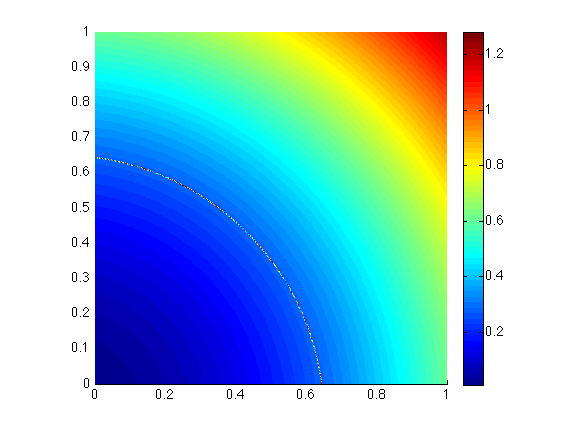
\includegraphics[width=\textwidth]{\assetsParentPath/assets/img/using-issm/tutorials/mesh/shock0.png}
	\end{center}
\end{figure}
First, we generate a simple uniform mesh. We interpolate the observations on the vertices of this mesh:
\begin{lstlisting}
>> md = bamg(model, 'domain', 'Square.exp', 'hmax', .05);
>> vel = shock(md.mesh.x, md.mesh.y);
>> plotmodel(md, 'data', vel, 'edgecolor', 'w');
\end{lstlisting}
\begin{figure}[H]
	\begin{center}
		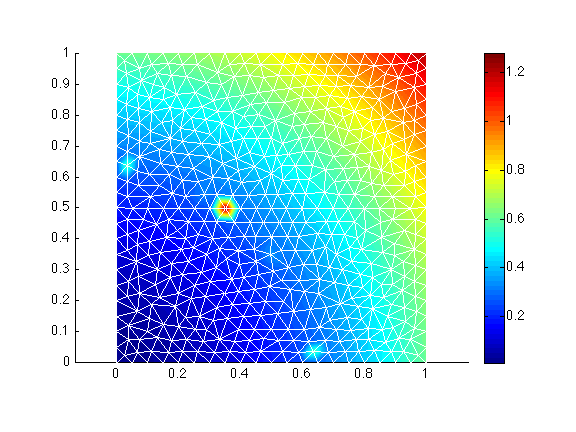
\includegraphics[width=\textwidth]{\assetsParentPath/assets/img/using-issm/tutorials/mesh/shock1.png}
	\end{center}
\end{figure}
With a simple uniform mesh, the discontinuity is not captured. It is best to start with a finer mesh, which captures the discontinuity rather well, and interpolate the observations on this finer mesh to adapt the mesh anisotropically.
\begin{lstlisting}
>> md = bamg(model, 'domain', 'Square.exp', 'hmax', .005);
>> vel = shock(md.mesh.x, md.mesh.y);
\end{lstlisting}
Now, we call \lstinlinebg|bamg| a second time to adapt the mesh according the \lstinlinebg|vel|. We do not reinitialize \lstinlinebg|md| and call \lstinlinebg|bamg| again without specifying the \lstinlinebg|'domain'|, as a first mesh already exists in the model. We provide the following options:
\begin{enumerate}
	\item \lstinlinebg|'field'| followed by \lstinlinebg|vel|, the field we want to adapt the mesh to
	\item \lstinlinebg|'err'| the allowed interpolation error (Here, the field must be captured within 0.05)
	\item \lstinlinebg|'hmin'| minimum edge length
	\item \lstinlinebg|'hmax'| maximum edge length
\end{enumerate}
\begin{lstlisting}
>> md = bamg(md, 'field', vel, 'err', 0.05, 'hmin', 0.005, 'hmax', 0.3);
>> vel = shock(md.mesh.x, md.mesh.y);
>> plotmodel(md, 'data', vel, 'edgecolor', 'w');
\end{lstlisting}
\begin{figure}[H]
	\begin{center}
		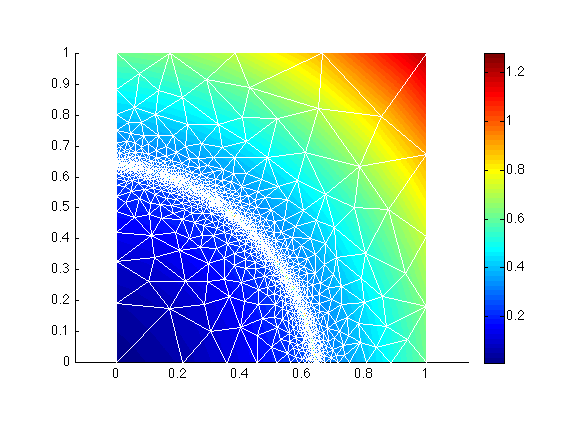
\includegraphics[width=\textwidth]{\assetsParentPath/assets/img/using-issm/tutorials/mesh/shock2.png}
	\end{center}
\end{figure}
You can change the option \lstinlinebg|'err'| to 0.03, to see the effect of \lstinlinebg|'err'|. The ratio between two consecutive edges can be controlled by the option \lstinlinebg|'gradation'|.
\begin{lstlisting}
>> md = bamg(model, 'domain', 'Square.exp', 'hmax', .005);
>> vel = shock(md.mesh.x, md.mesh.y);
>> md = bamg(md, 'field', vel, 'err', 0.03, 'hmin', 0.005, 'hmax', 0.3, 'gradation', 3);
>> vel = shock(md.mesh.x, md.mesh.y);
>> plotmodel(md, 'data', vel, 'edgecolor', 'w');
\end{lstlisting}
\begin{figure}[H]
	\begin{center}
		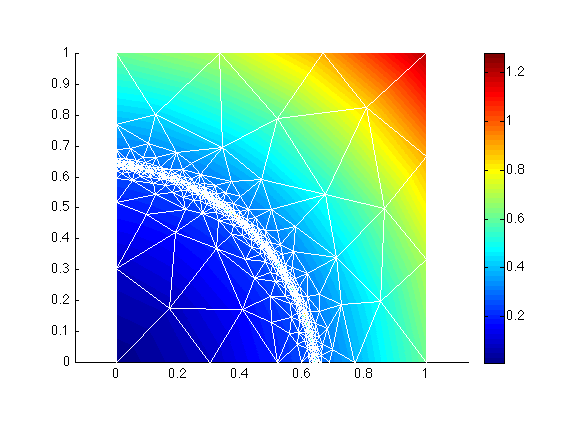
\includegraphics[width=\textwidth]{\assetsParentPath/assets/img/using-issm/tutorials/mesh/shock3.png}
	\end{center}
\end{figure}
We can also force the triangles to be equilateral by using the \lstinlinebg|'anisomax'| option, which specifies the maximum level of anisotropy (between 0 and 1, 1 being fully isotropic).
\begin{lstlisting}
>> md = bamg(model, 'domain', 'Square.exp', 'hmax', .005);
>> vel = shock(md.mesh.x, md.mesh.y);
>> md = bamg(md, 'field', vel, 'err', 0.03, 'hmin', 0.005, 'hmax', 0.3, 'gradation', 1.3, 'anisomax', 1);
>> vel = shock(md.mesh.x, md.mesh.y);
>> plotmodel(md, 'data', vel, 'edgecolor', 'w');
\end{lstlisting}
\begin{figure}[H]
	\begin{center}
		\includegraphics[width=\textwidth]{\assetsParentPath/assets/img/using-issm/tutorials/mesh/shock4.png}
	\end{center}
\end{figure}
You can also try to refine a mesh using the function \lstinlinebg|circles.m|, which is provided in the same directory.
%}}}

\paragraph{Mesh refinement in a specific region}%{{{
It is sometimes necessary to specify a mesh resolution for an area of interest. We will use the same example as before. The first step consists of creating an ARGUS file that defines the region where we want to refine the mesh.

We first plot \lstinlinebg|vel| and we call the function \lstinlinebg|exptool| to create a file \lstinlinebg|refinement.exp| that defines this region. Select \lstinlinebg|add a contour (closed)|. Draw a contour over a given region, hit enter when you are done, and then select quit. You should now see the \lstinlinebg|refinement.exp| file in the current directory.
\begin{lstlisting}
>> plotmodel(md, 'data', vel, 'edgecolor', 'w');
>> exptool('refinement.exp')
\end{lstlisting}
\begin{figure}[H]
	\begin{center}
		\includegraphics[width=\textwidth]{\assetsParentPath/assets/img/using-issm/tutorials/mesh/exptool.png}
	\end{center}
\end{figure}

Now, we are going to create a vector that specifies, for each vertex of the existing mesh, the resolution of the adapted mesh. We use \lstinlinebg|NaN| for the vertices we do not want to change. So in this example, this will be a vector of \lstinlinebg|NaN|, except for the vertices in \lstinlinebg|refinement.exp|, where we want a resolution of 0.02:
\begin{lstlisting}
>> h = NaN * ones(md.mesh.numberofvertices, 1);
>> in = ContourToNodes(md.mesh.x, md.mesh.y, 'refinement.exp', 1);
>> h(find(in)) = 0.02;
>> plotmodel(md, 'data', in, 'edgecolor', 'w');
\end{lstlisting}
You will see that all the vertices that are in \lstinlinebg|refinement.exp| have a value of 1 (they are inside the contour), and the others are 0.
\begin{figure}[H]
	\begin{center}
		\includegraphics[width=\textwidth]{\assetsParentPath/assets/img/using-issm/tutorials/mesh/refine1.png}
	\end{center}
\end{figure}

Now, we call \lstinlinebg|bamg| a third time, with the specified resolution for the vertices that are in \lstinlinebg|refinement.exp|:
\begin{lstlisting}
>> vel = shock(md.mesh.x, md.mesh.y);
>> md = bamg(md, 'field', vel, 'err', 0.03, 'hmin', 0.005, 'hmax', 0.3, 'hVertices', h);
>> vel = shock(md.mesh.x, md.mesh.y);
>> plotmodel(md, 'data', vel, 'edgecolor', 'w');
\end{lstlisting}
\begin{figure}[H]
	\begin{center}
		\includegraphics[width=\textwidth]{\assetsParentPath/assets/img/using-issm/tutorials/mesh/refine2.png}
	\end{center}
\end{figure}
%}}}

\paragraph{Another example}%{{{
If you would like to try another example, you can use the function \lstinlinebg|circles.m| instead of
\lstinlinebg|shock.m|. It is also a 1x1 square but with a pattern that includes five circles.
%}}}

\clearpage % Make sure all figures are placed before next section

% Just The Docs Front Matter
% title: Ice Flow Models
% parent: Tutorials
% has_children: false
% has_toc: false

\subsection{Ice Flow Models} \label{sec:using-issm-tutorials-iceflowmodels}
UNDER DEVELOPMENT

\clearpage % Make sure all figures are placed before next section

% Just The Docs Front Matter
% title: Ice Sheet Model Intercomparison Project (ISMIP) Tests
% parent: Tutorials
% has_children: false
% has_toc: false

\subsection{Ice Sheet Model Intercomparison Project (ISMIP) Tests} \label{sec:using-issm-tutorials-ismip}
\subsubsection{Goals} %{{{
\begin{itemize}
	\item Test the ISSM skills that you have gained so far
	\item Create ISSM models by Following the given keyword instructions
	\item Run tests from the Ice Sheet Model Intercomparison Project (ISMIP - Tests A and F) (see \href{https://tc.copernicus.org/articles/2/95/2008/}{publication} for more information about these tests)
\end{itemize}

Go to \lstinlinebg|<ISSM_DIR>/examples/ISMIP/| to do this tutorial.

%}}}
\subsubsection{Introduction/How To} %{{{
The \lstinlinebg|runme.m| file and \lstinlinebg|*par| files give a layout of the simulation that has to be modified.
\begin{itemize}
	\item Each code line that has to be typed in is preceded by \lstinlinebg|\%->|. Type the appropriate code below this symbol.
	\item Keywords introduced by \lstinlinebg|#| should be typed in MATLAB to get more information, if necessary
	\item See the solutions below if you get stuck.
\end{itemize}
%}}}

\subsubsection{Test A} %{{{
In Test A, we will generate a Square ice sheet flowing over a bumpy bed:
\begin{itemize}
	\item Sinusoidal bedrock
	\item Ice frozen on the bed
	\item Periodic boundary conditions
\end{itemize}
\begin{figure}[H]
	\begin{center}
		\includegraphics[width=\textwidth]{\assetsParentPath/assets/img/using-issm/tutorials/ismip/SquareIceFlow.png}
	\end{center}
\end{figure}
%}}}
\subsubsection{Simulation File Layout and Organization}  %{{{
The simulation file \lstinlinebg|runme.m| is organized into different steps, each with the same structure:
\begin{itemize}
	\item Model loading
	\item Performing an action
	\item Model saving
\end{itemize}
The step specifier \lstinlinebg|steps| is defined at the top of the \lstinlinebg|runme.m| file.
%}}}

\subsubsection{Mesh} %{{{
In place of loading a preceding model we initialize one. The action here is the generation of a mesh. To do this initialize \lstinlinebg|md| as a new model \lstinlinebg|(#help model)| and generate a \lstinlinebg|squaremesh| \lstinlinebg|(#help squaremesh)| with the following parameters. Afterward, plot the mesh and save the model.
\begin{itemize}
	\item Mesh size: 80,000 meters
	\item Nodes in each direction: 20
\end{itemize}
\begin{figure}[H]
	\begin{center}
		\includegraphics[width=\textwidth]{\assetsParentPath/assets/img/using-issm/tutorials/ismip/Mesh.png}
	\end{center}
\end{figure}
Load the preceding step \lstinlinebg|(#help loadmodel)|. Path is given by the organizer with the name of the given step. Set the mask \lstinlinebg|(#help setmask)|. Note that all MISMIP nodes are grounded. Plot the given mask \lstinlinebg|(md.mask)| to locate the field. Save the model.
\begin{itemize}
	\item Mesh size: 80,000 meters
	\item Nodes in each direction: 20
	\item All grounded: default
\end{itemize}
\begin{figure}[H]
	\begin{center}
		\includegraphics[width=\textwidth]{\assetsParentPath/assets/img/using-issm/tutorials/ismip/Mesh2.png}
	\end{center}
\end{figure}
%}}}
\subsubsection{Parameterization} %{{{
Load the preceding step. Next, parameterize the model \lstinlinebg|(#help parameterize)|. You will need to fill up the parameter file (given by the name ParamFile variable). Save the given model. It is important to note that the values are not important as we are dealing with a no-sliding flux. The values will be overridden by the basal boundary conditions. Take care of the size of the parameters.
\begin{itemize}
	\item Mesh size: 80,000 meters
	\item Nodes in each direction: 20
	\item All grounded: default
	\item Ice-flow parameter: \lstinlinebg|B = 6.8067 x 10^7 Pa s^1/n|
	\item Glen's exponent: n = 3
\end{itemize}
\begin{figure}[H]
	\begin{center}
		\includegraphics[width=\textwidth]{\assetsParentPath/assets/img/using-issm/tutorials/ismip/Parameterize1.png}
	\end{center}
\end{figure}
%}}}
\subsubsection{Extrusion} %{{{
Load \lstinlinebg|Parameterization| model. The action here is to extrude the preceding mesh. Next, vertically extrude the preceding mesh \lstinlinebg|(#help extrude)| with only 5 layers exponent 1. Plot the 3D geometry and save the model.
\begin{itemize}
	\item Mesh size: 80,000 meters
	\item Nodes in each direction: 20
	\item All grounded: default
	\item Ice-flow parameter: \lstinlinebg|B = 6.8067 x 10^7 Pa s^1/n|
	\item Glen's exponent: n = 3
	\item 5 layer extrusion
\end{itemize}
\begin{figure}[H]
	\begin{center}
		\includegraphics[width=\textwidth]{\assetsParentPath/assets/img/using-issm/tutorials/ismip/Extrusion1.png}
	\end{center}
\end{figure}
%}}}
\subsubsection{Flow Equation} %{{{
Load the \lstinlinebg|Extrusion| model and set the approximation for the flow computation \lstinlinebg|(#help setflowequation)|. We will be using the Higher Order Model (HO). Save the model.
\begin{itemize}
	\item Mesh size: 80,000 meters
	\item Nodes in each direction: 20
	\item All grounded: default
	\item Ice-flow parameter: \lstinlinebg|B = 6.8067 x 10^7 Pa s^1/n|
	\item Glen's exponent: n = 3
	\item 5 layers extrusion
	\item Flow model: HO
\end{itemize}
%}}}

\subsubsection{Boundary Conditions} %{{{
Load the \lstinlinebg|SetFlow| model. Dirichlet boundary condition are known as SPC's, where ice is frozen to the base with no velocity. SPC's are initialized at NaN one value per vertex. Extract the nodenumbers at the base \lstinlinebg|(#md.mesh.vertexonbase)| and set the sliding to zero on the bed (Vx and Vy). Periodic boundaries have to be fixed on the sides. Create tabs with the side of the domain for x, and create maxX \lstinlinebg|(#help find)|. This command give subsets of matrices based on boolean operations. Now create minX. For y, max X and min X should be excluded. Now create min Y. Set the node that should be paired together \lstinlinebg|(#md.stressbalance.vertex_pairing)|. If we are dealing with IsmipF the solution is in masstransport. Save the given model. \lstinlinebg|(#md.masstransport.vertex_pairing = md.stressbalance.vertex_pairing)|.
\begin{itemize}
	\item Mesh size: 80,000 meters
	\item Nodes in each direction: 20
	\item All grounded: default
	\item Ice-flow parameter: \lstinlinebg|B = 6.8067 x 10^6 Pa s^1/n|
	\item Glen's exponent: n = 3
	\item 5 layer extrusion
	\item Flow model: HO
\end{itemize}
%}}}

\subsubsection{Solve Model} %{{{
Load the \lstinlinebg|BoundaryConditions| model. Set the cluster \lstinlinebg|(#md.cluster)| with generic parameters \lstinlinebg|(#help generic)|. Set only the name and number of processes. Set which control message you want to see \lstinlinebg|(#help verbose.)| Solve \lstinlinebg|(#help solve)|. We are solving a StressBalance. Save the model, and plot the surface velocities.
\begin{itemize}
	\item Mesh size: 80,000 meters
	\item Nodes in each direction: 20
	\item All grounded: default
	\item Ice-flow parameter: \lstinlinebg|B = 6.8067 x 10^7 Pa s^1/n|
	\item Glen's exponent: n = 3
	\item 5 layers extrusion
	\item Flow model: HO
\end{itemize}
\begin{figure}[H]
	\begin{center}
		\includegraphics[width=\textwidth]{\assetsParentPath/assets/img/using-issm/tutorials/ismip/BoundaryCondition.png}
	\end{center}
\end{figure}
%}}}
\subsubsection{Test F} %{{{
Square ice sheet flowing over a bump.
\begin{itemize}
	\item Gaussian bumped bedrock
	\item Ice frozen or sliding on the bed
	\item Periodic boundary conditions
	\item Transient model until steady-state
\end{itemize}
\begin{figure}[H]
	\begin{center}
		\includegraphics[width=\textwidth]{\assetsParentPath/assets/img/using-issm/tutorials/ismip/RedSquareFlow.png}
	\end{center}
\end{figure}
\paragraph{Model Setup}
\begin{itemize}
	\item Mesh size: 100,000 meters
	\item Nodes in each direction: 30
	\item All grounded: default
	\item Ice-flow parameter: \lstinlinebg|B = 1.4734 x 10^14 Pa s^1/n| (or, \lstinlinebg|B = A^(-1/n)| where \lstinlinebg|n = 1| and \lstinlinebg|A = 2.140373 x 10^-7 Pa^-1 yr^-1|)
	\item Glen's exponent: n = 1
	\item 5 layers extrusion
	\item Flow model: HO
\end{itemize}
%}}}

\subsubsection{Actual Work and Results} %{{{
Load the preceding model under the path given by the organizer with the name of the given step. Set the cluster with generic parameters. Set only the name and number of the process. Set which control message you want to see. Set the transient model to ignore the thermal model \lstinlinebg|(#md.transient)|. Define the timestepping scheme. Everything here should be provided in years \lstinlinebg|(#md.timestepping)|. Give the length of the \lstinlinebg|time step| (4 years). Give the \lstinlinebg|final_time (20 * 4 years time_steps)|. Now solve, we are solving for TransientSolution. Lastly plot the surface velocities. Here is the upper surface velocity:

Side view:
\begin{figure}[H]
	\begin{center}
		\includegraphics[width=\textwidth]{\assetsParentPath/assets/img/using-issm/tutorials/ismip/UpperSurface2.png}
	\end{center}
\end{figure}
Top view:
\begin{figure}[H]
	\begin{center}
		\includegraphics[width=\textwidth]{\assetsParentPath/assets/img/using-issm/tutorials/ismip/UpperSurfaceVelocity.png}
	\end{center}
\end{figure}
%}}}
\subsubsection{Solution for runme.m (MATLAB)}%{{{
\begin{lstlisting}
%which steps to perform; steps are from 1 to 8
%step 7 is specific to ISMIPA
%step 8 is specific to ISMIPF

steps = [1:7]; %ISMIPA
%steps = [1:6, 8]; %ISMIPB

% parameter file to be used, choose between IsmipA.par or IsmipF.par
ParamFile = 'IsmipA.par'
%ParamFile = 'IsmipF.par'

%Run Steps

%Mesh Generation #1
if any(steps == 1)
	%initialize md as a new model #help model
	%->
	md = model();
	% generate a squaremesh #help squaremesh
	% Side is 80 km long with 20 points
	%->
	if(ParamFile == 'IsmipA.par'),
		md = squaremesh(md, 80000, 80000, 20, 20);
	elseif(ParamFile == 'IsmipF.par'),
		md = squaremesh(md, 100000, 100000, 30, 30);
	end
	% plot the given mesh #plotdoc
	%->
	plotmodel(md, 'data', 'mesh')
	% save the given model
	%->
	save ./Models/ISMIP.Mesh_generation md;
end

%Masks #2
if any(steps == 2)
	% load the preceding step #help loadmodel
	% path is given by the organizer with the name of the given step
	%->
	md = loadmodel('./Models/ISMIP.Mesh_generation');
	% set the mask #help setmask
	% all MISMIP nodes are grounded
	%->
	md = setmask(md, '', '');
	% plot the given mask #md.mask to locate the field
	%->
	plotmodel(md, 'data', md.mask.ocean_levelset);
	% save the given model
	%->
	save ./Models/ISMIP.SetMask md;
end

%Parameterization #3
if any(steps == 3)
	% load the preceding step #help loadmodel
	% path is given by the organizer with the name of the given step
	%->
	md = loadmodel('./Models/ISMIP.SetMask');
	% parametrize the model # help parameterize
	% you will need to fill up the parameter file defined by the
	% ParamFile variable
	%->
	md = parameterize(md, ParamFile);
	% save the given model
	%->
	save ./Models/ISMIP.Parameterization md;
end

%Extrusion #4
if any(steps == 4)
	
	% load the preceding step #help loadmodel
	% path is given by the organizer with the name of the given step
	%->
	md = loadmodel('./Models/ISMIP.Parameterization');
	% vertically extrude the preceding mesh #help extrude
	% only 5 layers exponent 1
	%->
	md = extrude(md, 5, 1);
	% plot the 3D geometry #plotdoc
	%->
	plotmodel(md, 'data', md.geometry.base)
	% save the given model
	%->
	save ./Models/ISMIP.Extrusion md;
end

%Set the flow computing method #5
if any(steps == 5)

	% load the preceding step #help loadmodel
	% path is given by the organizer with the name of the given step
	%->
	md = loadmodel('./Models/ISMIP.Extrusion');
	% set the approximation for the flow computation #help setflowequation
	% We will be using the Higher Order Model (HO)
	%->
	md = setflowequation(md, 'HO', 'all');
	% save the given model
	%->
	save ./Models/ISMIP.SetFlow md;
end

%Set Boundary Conditions #6
if any(steps == 6)

	% load the preceding step #help loadmodel
	% path is given by the organizer with the name of the given step
	%->
	md = loadmodel('./Models/ISMIP.SetFlow');
	% dirichlet boundary condition are known as SPCs
	% ice frozen to the base, no velocity	#md.stressbalance
	% SPCs are initialized at NaN one value per vertex
	%->
	md.stressbalance.spcvx = NaN * ones(md.mesh.numberofvertices, 1);
	%->
	md.stressbalance.spcvy = NaN * ones(md.mesh.numberofvertices, 1);
	%->
	md.stressbalance.spcvz = NaN * ones(md.mesh.numberofvertices, 1);
	% extract the nodenumbers at the base #md.mesh.vertexonbase
	%->
	basalnodes = find(md.mesh.vertexonbase);
	% set the sliding to zero on the bed
	%->
	md.stressbalance.spcvx(basalnodes) = 0.0;
	%->
	md.stressbalance.spcvy(basalnodes) = 0.0;
	% periodic boundaries have to be fixed on the sides
	% Find the indices of the sides of the domain, for x and then for y
	% for x
	% create maxX, list of indices where x is equal to max of x (use >> help find)
	%->
	maxX = find(md.mesh.x == max(md.mesh.x));
	% create minX, list of indices where x is equal to min of x
	%->
	minX = find(md.mesh.x == min(md.mesh.x));
	% for y
	% create maxY, list of indices where y is equal to max of y
	%  but not where x is equal to max or min of x
	% (i.e, indices in maxX and minX should be excluded from maxY and minY)
	%->
	maxY = find(md.mesh.y == max(md.mesh.y) & md.mesh.x ~= max(md.mesh.x) & md.mesh.x ~= min(md.mesh.x));
	% create minY, list of indices where y is equal to max of y
	% but not where x is equal to max or min of x
	%->
	minY = find(md.mesh.y == min(md.mesh.y) & md.mesh.x ~= max(md.mesh.x) & md.mesh.x ~= min(md.mesh.x));
	% set the node that should be paired together, minX with maxX and minY with maxY
	% #md.stressbalance.vertex_pairing
	%->
	md.stressbalance.vertex_pairing = [minX, maxX; minY, maxY];
	if (ParamFile == 'IsmipF.par')
		% if we are dealing with IsmipF the solution is in
		% masstransport
		md.masstransport.vertex_pairing = md.stressbalance.vertex_pairing;
	end
	% save the given model
	%->
	save ./Models/ISMIP.BoundaryCondition md;
end

%Solving #7
if any(steps == 7)
	% load the preceding step #help loadmodel
	% path is given by the organizer with the name of the given step
	%->
	md = loadmodel('./Models/ISMIP.BoundaryCondition');
	% Set cluster #md.cluster
	% generic parameters #help generic
	% set only the name and number of process
	%->
	md.cluster = generic('name', oshostname(), 'np', 2);
	% Set which control message you want to see #help verbose
	%->
	md.verbose = verbose('convergence', true);
	% Solve #help solve
	% we are solving a StressBalanc
	%->
	md = solve(md, 'Stressbalance');
	% save the given model
	%->
	save ./Models/ISMIP.StressBalance md;
	% plot the surface velocities #plotdoc
	%->
	plotmodel(md, 'data', md.results.StressbalanceSolution.Vel)
end

%Solving #8
if any(steps == 8)
	% load the preceding step #help loadmodel
	% path is given by the organizer with the name of the given step
	%->
	md = loadmodel('./Models/ISMIP.BoundaryCondition');
	% Set cluster #md.cluster
	% generic parameters #help generic
	% set only the name and number of process
	%->
	md.cluster = generic('name', oshostname(), 'np', 2);
	% Set which control message you want to see #help verbose
	%->
	md.verbose = verbose('convergence', true);
	% set the transient model to ignore the thermal model
	% #md.transient
	%->
	md.transient.isthermal = 0;
	% define the timestepping scheme
	% everything here should be provided in years #md.timestepping
	% give the length of the time_step (4 years)
	%->
	md.timestepping.time_step = 4;
	% give final_time (20 * 4 years time_steps)
	%->
	md.timestepping.final_time = 4 * 20;
	% Solve #help solve
	% we are solving a TransientSolution
	%->
	md = solve(md, 'Transient');
	% save the given model
	%->
	save ./Models/ISMIP.Transient md;
	% plot the surface velocities #plotdoc
	%->
	plotmodel(md, 'data', md.results.TransientSolution(20).Vel)
end
\end{lstlisting}
%}}}
\subsubsection{Solution for runme.m (Python)}%{{{
\begin{lstlisting}
import numpy as np
from model import *
from squaremesh import squaremesh
from plotmodel import plotmodel
from export_netCDF import export_netCDF
from loadmodel import loadmodel
from setmask import setmask
from parameterize import parameterize
from setflowequation import setflowequation
from socket import gethostname
from solve import solve

#which steps to perform; steps are from 1 to 8
#step 7 is specific to ISMIPA
#step 8 is specific to ISMIPF

steps = [1, 2, 3, 4, 5, 6, 8]

# parameter file to be used, choose between IsmipA_cor.py or IsmipF_cor.py
ParamFile = 'IsmipF_cor.py'

#Run Steps

#Mesh Generation #1
if 1 in steps:
    print("Now generating the mesh")
    #initialize md as a new model help(model)
    #->
    md = model()
    # generate a squaremesh help(squaremesh)
    # Side is 80 km long with 20 points
    #->
    if ParamFile == 'IsmipA_cor.py':
        md = squaremesh(md, 80000, 80000, 20, 20)
    elif ParamFile == 'IsmipF_cor.py':
        md = squaremesh(md, 100000, 100000, 30, 30)

    # plot the given mesh plotdoc()
    #->
    plotmodel(md, 'data', 'mesh', 'figure', 1)
    # save the given model
    #->
    export_netCDF(md, "./Models/ISMIP-Mesh_generation.nc")

#Masks #2
if 2 in steps:
    print("Setting the masks")
    # load the preceding step help(loadmodel)
    # path is given by the organizer with the name of the given step
    #->
    md = loadmodel("./Models/ISMIP-Mesh_generation.nc")
    # set the mask help(setmask)
    # all MISMIP nodes are grounded
    #->
    md = setmask(md, '', '')
    # plot the given mask #md.mask to locate the field
    #->
    plotmodel(md, 'data', md.mask.ocean_levelset, 'figure', 2)
    # save the given model
    #->
    export_netCDF(md, "./Models/ISMIP-SetMask.nc")

#Parameterization #3
if 3 in steps:
    print("Parameterizing")
    # load the preceding step #help loadmodel
    # path is given by the organizer with the name of the given step
    #->
    md = loadmodel("./Models/ISMIP-SetMask.nc")
    # parametrize the model # help parameterize
    # you will need to fill up the parameter file (given by the
    # ParamFile variable)
    #->
    md = parameterize(md, ParamFile)
    # save the given model
    #->
    export_netCDF(md, "./Models/ISMIP-Parameterization.nc")

#Extrusion #4
if 4 in steps:
    print("Extruding")
    # load the preceding step #help loadmodel
    # path is given by the organizer with the name of the given step
    #->
    md = loadmodel("./Models/ISMIP-Parameterization.nc")
    # vertically extrude the preceding mesh #help extrude
    # only 5 layers exponent 1
    #->
    md = md.extrude(5, 1)
    # plot the 3D geometry #plotdoc
    #->
    plotmodel(md, 'data', md.geometry.base, 'figure', 3)
    # save the given model
    #->
    export_netCDF(md, "./Models/ISMIP-Extrusion.nc")

#Set the flow computing method #5
if 5 in steps:
    print("setting flow approximation")
    # load the preceding step #help loadmodel
    # path is given by the organizer with the name of the given step
    #->
    md = loadmodel("./Models/ISMIP-Extrusion.nc")
    # set the approximation for the flow computation #help setflowequation
    # We will be using the Higher Order Model (HO)
    #->
    md = setflowequation(md, 'HO', 'all')
    # save the given model
    #->
    export_netCDF(md, "./Models/ISMIP-SetFlow.nc")

#Set Boundary Conditions #6
if 6 in steps:
    print("setting boundary conditions")
    # load the preceding step #help loadmodel
    # path is given by the organizer with the name of the given step
    #->
    md = loadmodel("./Models/ISMIP-SetFlow.nc")
    # dirichlet boundary condition are known as SPCs
    # ice frozen to the base, no velocity   #md.stressbalance
    # SPCs are initialized at NaN one value per vertex
    #->
    md.stressbalance.spcvx = np.nan * np.ones((md.mesh.numberofvertices))
    #->
    md.stressbalance.spcvy = np.nan * np.ones((md.mesh.numberofvertices))
    #->
    md.stressbalance.spcvz = np.nan * np.ones((md.mesh.numberofvertices))
    # extract the nodenumbers at the base #md.mesh.vertexonbase
    #->
    basalnodes = np.nonzero(md.mesh.vertexonbase)
    # set the sliding to zero on the bed (Vx and Vy)
    #->
    md.stressbalance.spcvx[basalnodes] = 0.0
    #->
    md.stressbalance.spcvy[basalnodes] = 0.0
    # periodic boundaries have to be fixed on the sides
    # Find the indices of the sides of the domain, for x and then for y
    # for x
    # create maxX, list of indices where x is equal to max of x (use >> help find)
    #->
    maxX = np.squeeze(np.nonzero(md.mesh.x == np.nanmax(md.mesh.x)))
    # create minX, list of indices where x is equal to min of x
    #->
    minX = np.squeeze(np.nonzero(md.mesh.x == np.nanmin(md.mesh.x)))
    # for y
    # create maxY, list of indices where y is equal to max of y
    # but not where x is equal to max or min of x
    # (i.e, indices in maxX and minX should be excluded from maxY and minY)
    #->
    maxY = np.squeeze(np.nonzero(np.logical_and.reduce((md.mesh.y == np.nanmax(md.mesh.y), md.mesh.x != np.nanmin(md.mesh.x), md.mesh.x != np.nanmax(md.mesh.x)))))
    # create minY, list of indices where y is equal to max of y
    # but not where x is equal to max or min of x
    #->
    minY = np.squeeze(np.nonzero(np.logical_and.reduce((md.mesh.y == np.nanmin(md.mesh.y), md.mesh.x != np.nanmin(md.mesh.x), md.mesh.x != np.nanmax(md.mesh.x)))))
    # set the node that should be paired together, minX with maxX and minY with maxY
    # #md.stressbalance.vertex_pairing
    #->
    md.stressbalance.vertex_pairing = np.hstack((np.vstack((minX + 1, maxX + 1)), np.vstack((minY + 1, maxY + 1)))).T
    if ParamFile == 'IsmipF_cor.py':
        # if we are dealing with IsmipF the solution is in masstransport
        md.masstransport.vertex_pairing = md.stressbalance.vertex_pairing

    # save the given model
    #->
    export_netCDF(md, "./Models/ISMIP-BoundaryCondition.nc")

#Solving #7
if 7 in steps:
    print("running the solver for the A case")
    # load the preceding step #help loadmodel
    # path is given by the organizer with the name of the given step
    #->
    md = loadmodel("./Models/ISMIP-BoundaryCondition.nc")
    # Set cluster #md.cluster
    # generic parameters #help generic
    # set only the name and number of process
    #->
    md.cluster = generic('name', gethostname(), 'np', 2)
    # Set which control message you want to see #help verbose
    #->
    md.verbose = verbose('convergence', True)
    # Solve #help solve
    # we are solving a StressBalance
    #->
    md = solve(md, 'Stressbalance')
    # save the given model
    #->
    export_netCDF(md, "./Models/ISMIP-StressBalance.nc")
    # plot the surface velocities #plotdoc
    #->
    plotmodel(md, 'data', md.results.StressbalanceSolution.Vel, 'figure', 4)

#Solving #8
if 8 in steps:
    print("running the solver for the F case")
    # load the preceding step #help loadmodel
    # path is given by the organizer with the name of the given step
    #->
    md = loadmodel("./Models/ISMIP-BoundaryCondition.nc")
    # Set cluster #md.cluster
    # generic parameters #help generic
    # set only the name and number of process
    #->
    md.cluster = generic('name', gethostname(), 'np', 2)
    # Set which control message you want to see #help verbose
    #->
    md.verbose = verbose('convergence', True)
    # set the transient model to ignore the thermal model
    # #md.transient
    #->
    md.transient.isthermal = 0
    # define the timestepping scheme
    # everything here should be provided in years #md.timestepping
    # give the length of the time_step (4 years)
    #->
    md.timestepping.time_step = 1
    # give final_time (20 * 4 years time_steps)
    #->
    md.timestepping.final_time = 1 * 20
    # Solve #help solve
    # we are solving a TransientSolution
    #->
    md = solve(md, 'Transient')
    # save the given model
    #->
    export_netCDF(md, "./Models/ISMIP-Transient.nc")
    # plot the surface velocities #plotdoc
    #->
    plotmodel(md, 'data', md.results.TransientSolution[19].Vel, 'layer', 5, 'figure', 5)
\end{lstlisting}
%}}}
\subsubsection{Solution for IsmipA.par (MATLAB)}%{{{
\begin{lstlisting}
%Parameterization for ISMIP A experiment

%Set the Simulation generic name #md.miscellaneous
%->

%Geometry
disp('   Constructing Geometry');

%Define the geometry of the simulation #md.geometry
%surface is [-x * tan(0.5 * pi / 180)] #md.mesh
%->
md.geometry.surface = -md.mesh.x * tan(0.5 * pi / 180.);
%base is [surface - 1000 + 500 * sin(x * 2 * pi / L) .* sin(y * 2 * pi / L)]
%L is the size of the side of the square #max(md.mesh.x) - min(md.mesh.x)
%->
L = max(md.mesh.x) - min(md.mesh.x);
md.geometry.base = md.geometry.surface - 1000.0 + 500.0 * sin(md.mesh.x * 2.0 * pi / L) .* sin(md.mesh.y * 2.0 * pi / L);
%thickness is the difference between surface and base #md.geometry
%->
md.geometry.thickness = md.geometry.surface - md.geometry.base;
%plot the geometry to check it out
%->
plotmodel(md, 'data', md.geometry.thickness);

disp('   Defining friction parameters');

%These parameters will not be used but need to be fixed #md.friction
%one friction coefficient per node (md.mesh.numberofvertices, 1)
%->
md.friction.coefficient = 200.0 * ones(md.mesh.numberofvertices, 1);
%one friction exponent (p, q) per element
%->
md.friction.p = ones(md.mesh.numberofelements, 1);
%->
md.friction.q = ones(md.mesh.numberofelements, 1);

disp('   Construct ice rheological properties');

%The rheology parameters sit in the material section #md.materials
%B has one value per vertex
%->
md.materials.rheology_B = 6.8067e7 * ones(md.mesh.numberofvertices, 1);
%n has one value per element
%->
md.materials.rheology_n = 3 * ones(md.mesh.numberofelements, 1);

disp('   Set boundary conditions');

%Set the default boundary conditions for an ice-sheet
% #help SetIceSheetBC
%->
md = SetIceSheetBC(md);
\end{lstlisting}
%}}}
\subsubsection{Solution for IsmipA.py (Python)}%{{{
\begin{lstlisting}


\end{lstlisting}
%}}}
\subsubsection{Solution for IsmipF.par (MATLAB)}%{{{
\begin{lstlisting}
%Parameterization for ISMIP F experiment

%Set the Simulation generic name #md.miscellaneous
%->

%Geometry
disp('   Constructing Geometry');

%Define the geometry of the simulation #md.geometry
%surface is [-x * tan(3.0 * pi / 180)] #md.mesh
%->
md.geometry.surface = -md.mesh.x * tan(3.0 * pi / 180.0);
%base is [surface - 1000 + 100 * exp(-((x - L / 2) .^ 2 + (y - L / 2) .^ 2) / (10000.^2))]
%L is the size of the side of the square #max(md.mesh.x) - min(md.mesh.x)
%->
L = max(md.mesh.x) - min(md.mesh.x);
%->
md.geometry.base = md.geometry.surface - 1000.0 + 100.0 * exp(-((md.mesh.x - L / 2.0) .^ 2.0 + (md.mesh.y - L / 2.0) .^ 2.0) / (10000.^2.0));
%thickness is the difference between surface and base #md.geometry
%->
md.geometry.thickness = md.geometry.surface - md.geometry.base;
%plot the geometry to check it out
%->
plotmodel(md, 'data', md.geometry.thickness);

disp('   Defining friction parameters');

%These parameters will not be used but need to be fixed #md.friction
%one friction coefficient per node (md.mesh.numberofvertices, 1)
%conversion form year to seconds with #md.constants.yts
%->
md.friction.coefficient = sqrt(md.constants.yts / (1000 * 2.140373 * 10^-7)) * ones(md.mesh.numberofvertices, 1);
%one friction exponent (p, q) per element
%->
md.friction.p = ones(md.mesh.numberofelements, 1);
%->
md.friction.q = zeros(md.mesh.numberofelements, 1);

disp('   Construct ice rheological properties');

%The rheology parameters sit in the material section #md.materials
%B has one value per vertex
%->
md.materials.rheology_B = (1 / (2.140373 * 10^-7 / md.constants.yts)) * ones(md.mesh.numberofvertices, 1);
%n has one value per element
%->
md.materials.rheology_n = 1 * ones(md.mesh.numberofelements, 1);

disp('   Set boundary conditions');

%Set the default boundary conditions for an ice-sheet
% #help SetIceSheetBC
%->
md = SetIceSheetBC(md);

disp('   Initializing velocity and pressure');

%initialize the velocity and pressurefields of #md.initialization
%->
md.initialization.vx = zeros(md.mesh.numberofvertices, 1);
%->
md.initialization.vy = zeros(md.mesh.numberofvertices, 1);
%->
md.initialization.vz = zeros(md.mesh.numberofvertices, 1);
%->
md.initialization.pressure = zeros(md.mesh.numberofvertices, 1);
\end{lstlisting}
%}}}
\subsubsection{Solution for IsmipF.py (Python)}%{{{
\begin{lstlisting}
import numpy as np
from plotmodel import plotmodel
from SetIceSheetBC import SetIceSheetBC
#Parameterization for ISMIP F experiment

#Set the Simulation generic name #md.miscellaneous
#->
md.miscellaneous.name = 'IsmipF_cor'
#Geometry
print('   Constructing Geometry')

#Define the geometry of the simulation #md.geometry
#surface is [-x * tan(3.0 * pi / 180)] #md.mesh
#->
md.geometry.surface = md.mesh.x * np.tan(3.0 * np.pi / 180.0)
#base is [surface - 1000 + 100 * exp(-((x - L / 2) .^ 2 + (y - L / 2) .^ 2) / (10000.^2))]
#L is the size of the side of the square #max(md.mesh.x) - min(md.mesh.x)
#->
L = np.nanmax(md.mesh.x) - np.nanmin(md.mesh.x)
#->
md.geometry.base = md.geometry.surface - 1000.0 + 100.0 * np.exp(-((md.mesh.x - L / 2.0) ** 2.0 + (md.mesh.y - L / 2.0) ** 2.0) / (10000.**2.0))
#thickness is the difference between surface and base #md.geometry
#->
md.geometry.thickness = md.geometry.surface - md.geometry.base
#plot the geometry to check it out
#->
plotmodel(md, 'data', md.geometry.thickness)

print('   Defining friction parameters')

#These parameters will not be used but need to be fixed #md.friction
#one friction coefficient per node (md.mesh.numberofvertices,1)
#conversion form year to seconds with #md.constants.yts
#->
md.friction.coefficient = np.sqrt(md.constants.yts / (1000 * 2.140373 * 1e-7)) * np.ones((md.mesh.numberofvertices))
#one friction exponent (p, q) per element
#->
md.friction.p = np.ones((md.mesh.numberofelements))
#->
md.friction.q = np.zeros((md.mesh.numberofelements))

print('   Construct ice rheological properties')

#The rheology parameters sit in the material section #md.materials
#B has one value per vertex
#->
md.materials.rheology_B = (1 / (2.140373 * 1e-7 / md.constants.yts)) * np.ones((md.mesh.numberofvertices))
#n has one value per element
#->
md.materials.rheology_n = np.ones((md.mesh.numberofelements))

print('   Set boundary conditions')

#Set the default boundary conditions for an ice-sheet
# #help SetIceSheetBC
#->
md = SetIceSheetBC(md)

print('   Initializing velocity and pressure')

#initialize the velocity and pressurefields of #md.initialization
#->
md.initialization.vx = np.zeros((md.mesh.numberofvertices))
#->
md.initialization.vy = np.zeros((md.mesh.numberofvertices))
#->
md.initialization.vz = np.zeros((md.mesh.numberofvertices))
#->
md.initialization.pressure = np.zeros((md.mesh.numberofvertices))
\end{lstlisting}
%}}}

\clearpage % Make sure all figures are placed before next section

% Just The Docs Front Matter
% title: Inversions
% parent: Tutorials
% has_children: false
% has_toc: false

\subsection{Inversions} \label{sec:using-issm-tutorials-inversions}
\subsubsection{Goals} %{{{
\begin{itemize}
	\item Learn how to use the model to invert for ice rigidity (B) and basal friction from surface velocities
	\item Being able to choose the right cost functions, with the right weights
	\item Understand the limitations of inversions
\end{itemize}
%}}}

\subsubsection{Introduction}%{{{
Several model input parameters, such as the ice rigidity $B$ (\lstinlinebg|md.materials.rheology_B|) and basal friction $\alpha$ (\lstinlinebg|md.friction.coefficient|), are difficult to measure remotely and are critical controls on ice dynamics.

To get a good guess of what these parameters are, we use \emph{inversions}. Inversions consist in inferring unknown parameters using additional observations. Here, we use surface velocities to infer our unknown input parameters, by minimizing the misfit between the observed and modeled velocities.

For example, our cost function could be:
\begin{equation}
	{\mathcal J\left({\bf v}\right)}
	=\int_{S} \dfrac{1}{2}\left(
	\left(v_x-v_x^{\text{obs}}\right)^{2}
	+\left(v_y-v_y^{\text{obs}}\right)^{2}
	\right) dS
\end{equation}
And so we would optimize our unknown model input to minimize the cost function ${\mathcal J}$.

Inversions were first introduced to glaciology by \cite{MacAyeal1993a} for an SSA model, and extended since to 3D models for other model parameters.

To illustrate this method, we are going to perform a twin experiment. We give ourselves a rigidity field (B) and use the modeled velocities as synthetic observation in a second run, where we start from another initial rigidity field, and see if we can recover the rigidity field that was used to generate the observations.
%}}}
\subsubsection{Hands on 1 (ice rigidity, B)} %{{{
\paragraph{Step 1: Generating Observations}
First, go to \lstinlinebg|<ISSM_DIR>/examples/Inversion/| and start MATLAB. We will start by creating a new model and generate our synthetic observations. Open the \lstinlinebg|runme.m| and ensure that \lstinlinebg|step = 1| at the top of the file. Execute this first step:
\begin{lstlisting}
>> runme
\end{lstlisting}
You will see on the left our prescribed rigidity, $B$, and to the right the calculated velocities. We choose a pattern with 2 distinct values for $B$ for the upper left region, and stiffer ice for the lower right, with a sharp transition.
\begin{figure}[H]
	\begin{center}
		\includegraphics[width=\textwidth]{\assetsParentPath/assets/img/using-issm/tutorials/inversion/step1.png}
	\end{center}
\end{figure}
In the next step, we our going to change the rigidity to something uniform, use our previously calculated velocities (from step 1) as observations, and see if we can recover that initial pattern that was used to generate the observations.

\paragraph{Step 2: Initial guess and initial velocity}
We now change the rigidity, $B$, and make it uniform. The results of the previous step are taken as observations (but we will only use them in step 3). Open \lstinlinebg|runme.m| and set \lstinlinebg|step = 2|. Save the file and execute step 2 in MATLAB as above.
\begin{figure}[H]
	\begin{center}
		\includegraphics[width=\textwidth]{\assetsParentPath/assets/img/using-issm/tutorials/inversion/step2.png}
	\end{center}
\end{figure}
We now see that the left panel is constant, and the velocity is symmetrical. This is our initial guess for $B$ and our initial modeled velocity. In the next step, we are going to tune $B$, so that the modeled velocity is as close as possible to the velocity of step 1.

\paragraph{Step 3: Inverting for B}
We perform here the inversion of $B$. Open \lstinlinebg|runme.m| and set the step as \lstinlinebg|step = 3|.
\begin{figure}[H]
	\begin{center}
		\includegraphics[width=\textwidth]{\assetsParentPath/assets/img/using-issm/tutorials/inversion/step3.png}
	\end{center}
\end{figure}
The general pattern is right (stiffer ice in the lower right), but it is noisy. Inverse problems are ill-posed: a solution might not exist, might not be unique, and might not depend continuously on input data. One of the consequences is that the inferred pattern for $B$ is not smooth, and these wiggles are \emph{not} physical. Adding regularization that penalizes wiggles in the control parameter stabilizes the inversion.

\paragraph{Step 4: Adding regularization}
Here, we would like to add a term of regularization to our cost function:
\begin{equation}
	{\mathcal J\left(B\right)}
	=
	\int_{S} w_1 \dfrac{1}{2}\left(
	\left(v_x-v_x^{\text{obs}}\right)^{2}
	+\left(v_y-v_y^{\text{obs}}\right)^{2}
	\right) dS
	+
	\int_{b} w_2 \dfrac{1}{2}
	\|\nabla B \|^{2}
	db
\end{equation}
The second term, known as Tikhonov regularization, penalizes strong gradients in $B$. Since the inversion tries to minimize our cost function $\mathcal J$, the optimization algorithm will try to also reduce the second term.

$w_1$ and $w_2$ are the weights associated to each component of the cost function. To have more regularization, one should increase $w_2$ (or decrease $w_1$), and vice versa.

Set \lstinlinebg|step = 4| in the \lstinlinebg|runme.m| file and execute it. Your results should now look like this:
\begin{figure}[H]
	\begin{center}
		\includegraphics[width=\textwidth]{\assetsParentPath/assets/img/using-issm/tutorials/inversion/step4.png}
	\end{center}
\end{figure}
We successfully reconstructed the pattern of ice rigidity, but we could not capture the sharp transition between high and low rigidity because of the regularization that we had to introduce to stabilize the inversion.
%}}}
\subsubsection{Hands on 2 (friction)} %{{{
We would like to do the same twin experiment here, but invert for basal friction of a grounded glacier. Here, you are going to make additions and/or modifications to the \lstinlinebg|runme.m| script as described below.

\paragraph{Changes to step 1}
\begin{enumerate}
	\item The mask is now all grounded
	\item Increase bed (\lstinlinebg|md.geometry.base|) and surface elevation (\lstinlinebg|md.geometry.surface|) by 100 meters
	\item $B$ (\lstinlinebg|md.materials.rheology_B|) is now uniform = 1.8x10\textsuperscript{8}
	\item Friction coefficient: 50, and 10 for 400,000\verb|<|x\verb|<|600,000
	\item change the \lstinlinebg|plotmodel| command and plot \lstinlinebg|md.friction.coefficient| instead, between 0 and 100.
\end{enumerate}
After running step 1 again, you should get the following figure.
\begin{figure}[H]
	\begin{center}
		\includegraphics[width=\textwidth]{\assetsParentPath/assets/img/using-issm/tutorials/inversion/step1b.png}
	\end{center}
\end{figure}
If you don't, then double check your changes before looking at the solutions below. We are modeling here a glacier flowing over a region where there is a lot of sliding. We want to see if the inversion can reconstruct this region of low friction.

\paragraph{Solutions to step 1 (MATLAB)}
\begin{lstlisting}
%Generate observations
md = model;
md = triangle(md, 'DomainOutline.exp', 100000);

%CHANGES START
md = setmask(md, '', '');
%CHANGES END

md = parameterize(md, 'Square.par');

%CHANGES START
md.geometry.base = md.geometry.base + 100;
md.geometry.surface = md.geometry.surface + 100;
md.materials.rheology_B(:) = 1.8e8;
md.friction.coefficient(:) = 50;
pos = find(md.mesh.x > 400e3 & md.mesh.x < 600e3);
md.friction.coefficient(pos) = 10;
%CHANGES END

md = setflowequation(md, 'SSA', 'all');
md.cluster = generic('np', 2);
md = solve(md, 'Stressbalance');

%CHANGES START
plotmodel(md, 'axis#all', 'tight', 'data', md.friction.coefficient, 'caxis', [0 100], 'title', '"True" coef', ...
   'data', md.results.StressbalanceSolution.Vel, 'title', '"observed velocities"')
%CHANGES END

save model1 md
\end{lstlisting}

\paragraph{Solutions to step 1 (Python)}
\begin{lstlisting}
import numpy as np
from model import *
from setmask import setmask
from parameterize import parameterize
from setflowequation import setflowequation
from generic import generic
from solve import solve
from plotmodel import plotmodel
from export_netCDF import export_netCDF
from m1qn3inversion import m1qn3inversion
from verbose import verbose
from loadmodel import loadmodel
from cuffey import cuffey

steps = [5]
Clims = [1.3 * 1e8, 1.9 * 1e8]

if 1 in steps:
    #Generate observations
    md = model()
    md = triangle(md, 'DomainOutline.exp', 100000)
    #CHANGES START
    md = setmask(md, '', '')
    #CHANGES END
    md = parameterize(md, 'Square.py')
    #CHANGES START
    md.geometry.base = md.geometry.base + 100.
    md.geometry.surface = md.geometry.surface + 100.
    md.friction.coefficient[:] = 50
    pos = np.nonzero(np.logical_and(md.mesh.x > 400e3, md.mesh.x < 600e3))
    md.friction.coefficient[pos] = 10
    #CHANGES END

    md = setflowequation(md, 'SSA', 'all')
    md.cluster = generic('np', 2)
    md = solve(md, 'Stressbalance')
    #CHANGES START
    plotmodel(md, 'axis#all', 'tight', 'data', md.friction.coefficient, 'caxis', [0, 100], 'title', '"True" coef', 'data', md.results.StressbalanceSolution.Vel, 'title', '"observed velocities"')
    #CHANGES END

    export_netCDF(md, 'model1.nc')

if 2 in steps:
    #Modify rheology, now constant
    md = loadmodel('model1.nc')
    md.materials.rheology_B[:] = 1.8 * 1e8

    #results of previous run are taken as observations
    md.inversion = m1qn3inversion()
    md.inversion.vx_obs = md.results.StressbalanceSolution.Vx
    md.inversion.vy_obs = md.results.StressbalanceSolution.Vy
    md.inversion.vel_obs = md.results.StressbalanceSolution.Vel

    #CHANGES START
    md.friction.coefficient[:] = 50
    #CHANGES END

    md = solve(md, 'Stressbalance')
    #CHANGES START
    plotmodel(md, 'axis#all', 'tight', 'data', md.friction.coefficient, 'caxis', [0, 100], 'title', '"True" coef', 'data', md.results.StressbalanceSolution.Vel, 'title', '"observed velocities"')
    #CHANGES END
    export_netCDF(md, 'model2.nc')

if 3 in steps:
    #invert for ice rigidity
    md = loadmodel('model2.nc')

    #Set up inversion parameters
    maxsteps = 20
    md.inversion.iscontrol = 1
    #CHANGES START
    md.inversion.control_parameters = ['FrictionCoefficient']
    #CHANGES END
    md.inversion.maxsteps = maxsteps
    md.inversion.cost_functions = [101]
    md.inversion.cost_functions_coefficients = np.ones((md.mesh.numberofvertices, 1))
    #CHANGES START
    md.inversion.min_parameters = np.ones((md.mesh.numberofvertices, 1))
    md.inversion.max_parameters = 100. * np.ones((md.mesh.numberofvertices, 1))
    #CHANGES END

    #Go solve!
    md.verbose = verbose(0)
    md = solve(md, 'Stressbalance')
    #CHANGES START
    plotmodel(md, 'axis#all', 'tight', 'data', md.results.StressbalanceSolution.FrictionCoefficient, 'caxis', [0, 100], 'title', '"True" coef', 'data', md.results.StressbalanceSolution.Vel, 'title', '"observed velocities"')
    #CHANGES END

if 4 in steps:
    #invert for ice rigidity
    md = loadmodel('model2.nc')

    #Set up inversion parameters
    maxsteps = 20
    md.inversion.iscontrol = 1
    md.inversion.control_parameters = ['FrictionCoefficient']
    md.inversion.maxsteps = maxsteps
    #CHANGES START
    md.inversion.cost_functions = [101, 103]
    md.inversion.cost_functions_coefficients = np.ones((md.mesh.numberofvertices, 2))
    md.inversion.cost_functions_coefficients[:, 0] = 3000
    md.inversion.cost_functions_coefficients[:, 1] = 1
    #CHANGES END
    md.inversion.min_parameters = np.ones((md.mesh.numberofvertices, 1))
    md.inversion.max_parameters = 100. * np.ones((md.mesh.numberofvertices, 1))

    #Go solve!
    md.verbose = verbose(0)
    md = solve(md, 'Stressbalance')
    #CHANGES START
    plotmodel(md, 'axis#all', 'tight', 'data', md.results.StressbalanceSolution.FrictionCoefficient, 'caxis', [0, 100], 'title', '"True" coef', 'data', md.results.StressbalanceSolution.Vel, 'title', '"observed velocities"')
    #CHANGES END

if 5 in steps:
    #invert for ice rigidity
    md = loadmodel('model2.nc')

    #Set up inversion parameters
    maxsteps = 20
    md.inversion.iscontrol = 1
    md.inversion.control_parameters = ['FrictionCoefficient']
    md.inversion.maxsteps = maxsteps
    #CHANGES START
    md.inversion.cost_functions = [101, 103, 501]
    md.inversion.cost_functions_coefficients = np.ones((md.mesh.numberofvertices, 3))
    #CHANGES END
    md.inversion.cost_functions_coefficients[:, 0] = 3000
    md.inversion.cost_functions_coefficients[:, 1] = 1
    #CHANGES START
    md.inversion.cost_functions_coefficients[:, 2] = 0.01
    #CHANGES END
    md.inversion.min_parameters = np.ones((md.mesh.numberofvertices, 1))
    md.inversion.max_parameters = 100. * np.ones((md.mesh.numberofvertices, 1))

    #Go solve!
    md.verbose = verbose(0)
    md = solve(md, 'Stressbalance')
    plotmodel(md, 'axis#all', 'tight', 'data', md.results.StressbalanceSolution.FrictionCoefficient, 'caxis', [0, 100], 'title', 'inferred B', 'data', md.results.StressbalanceSolution.Vel, 'title', 'modeled velocities')
\end{lstlisting}

\paragraph{Changes to step 2}
For step 2, we now want to set our new first guess for the basal friction to a uniform value.
\begin{enumerate}
	\item set the friction (\lstinlinebg|md.friction.coefficient|) to a uniform value of 50
	\item change the \lstinlinebg|plotmodel| command and plot \lstinlinebg|md.friction.coefficient| instead, between 0 and 100.
\end{enumerate}
After running step 2, you should get the following figure:
\begin{figure}[H]
	\begin{center}
		\includegraphics[width=\textwidth]{\assetsParentPath/assets/img/using-issm/tutorials/inversion/step2b.png}
	\end{center}
\end{figure}
if you don't, double check your changes. As you can see, the velocity does not show any fast flowing ice stream in the center of the domain, as expected since the friction is uniform.

\paragraph{Solutions to step 2}
\begin{lstlisting}
%Modify rheology, now constant
loadmodel('model1.mat');
md.materials.rheology_B(:) = 1.8 * 10^8;

%results of previous run are taken as observations
md.inversion = m1qn3inversion();
md.inversion.vx_obs		= md.results.StressbalanceSolution.Vx;
md.inversion.vy_obs		= md.results.StressbalanceSolution.Vy;
md.inversion.vel_obs	= md.results.StressbalanceSolution.Vel;

%CHANGES START
md.friction.coefficient(:) = 50;
%CHANGES END

md = solve(md, 'Stressbalance');
%CHANGES START
plotmodel(md, 'axis#all', 'tight', 'data', md.friction.coefficient, 'caxis', [0 100], 'title', 'coeff first guess', ...
	'data', md.results.StressbalanceSolution.Vel, 'title', 'modeled velocities')
%CHANGES END
save model2 md
\end{lstlisting}

\paragraph{Changes to step 3}
We now want to invert for basal friction and see if we can reconstruct the zone of sliding. We need to change what we are inverting for, and change the optimization parameters:
\begin{itemize}
	\item We now invert for \lstinlinebg|'FrictionCoefficient'|
	\item Do we keep the same cost function? yes for now...
	\item We want the parameter to be between 1 and 100
\end{itemize}
After running step 3, you should get the following figure:
\begin{figure}[H]
	\begin{center}
		\includegraphics[width=\textwidth]{\assetsParentPath/assets/img/using-issm/tutorials/inversion/step3b.png}
	\end{center}
\end{figure}
if you don't, the solutions are as follows,

\paragraph{Solutions to step 3}
\begin{lstlisting}
%invert for ice rigidity
loadmodel('model2.mat');

%Set up inversion parameters
maxsteps = 20;
md.inversion.iscontrol = 1;
%CHANGES START
md.inversion.control_parameters = {'FrictionCoefficient'};
%CHANGES END
md.inversion.maxsteps = maxsteps;
md.inversion.cost_functions = 101;
md.inversion.cost_functions_coefficients = ones(md.mesh.numberofvertices, 1);
%CHANGES START
md.inversion.min_parameters = ones(md.mesh.numberofvertices, 1);
md.inversion.max_parameters = 100*ones(md.mesh.numberofvertices, 1);
%CHANGES END

%Go solve!
md.verbose = verbose(0);
md = solve(md, 'Stressbalance');
%CHANGES START
plotmodel(md, 'axis#all', 'tight', 'data', md.results.StressbalanceSolution.FrictionCoefficient, 'caxis' , [0 100], 'title', 'inferred coeff', ...
	'data', md.results.StressbalanceSolution.Vel, 'title', 'modeled velocities')
%CHANGES END
\end{lstlisting}

As you can see, we get more sliding close to the front, but the rest of the domain is unchanged. That's because when we look at the velocity (right), it does capture the fast spot close to the front, so in terms of cost function, the inversion did a great job in matching the observation. But if we look at the log of the velocity (note, we are adding one to avoid \lstinlinebg|log(0)|):
\begin{lstlisting}
plotmodel(md, 'data', md.inversion.vel_obs + 1, 'data', md.results.StressbalanceSolution.Vel + 1, 'log#all', 10, 'caxis#all', [1 400])
\end{lstlisting}
\begin{figure}[H]
	\begin{center}
		\includegraphics[width=\textwidth]{\assetsParentPath/assets/img/using-issm/tutorials/inversion/step3b_log.png}
	\end{center}
\end{figure}
we clearly see the zone of fast sliding in the observations but not in the results from the inversion. So we need to change the cost function to add this information, we not only want the square of the difference between modeled and observed velocities to be minimized, we also want their logs to be minimized.

\paragraph{Changing the cost function}
We want the cost function to include an additional term:
\begin{equation}
	{\mathcal J\left({\bf v}\right)}
	=\int_{S} w_1 \dfrac{1}{2}\left(
	\left(v_x-v_x^{\text{obs}}\right)^{2}
	+\left(v_y-v_y^{\text{obs}}\right)^{2}
	\right) dS
	+\int_{S} w_2 \left(\text{log}\left(
	\dfrac{\|{\bf v}\|+\varepsilon}{\|{\bf v}^{\text{obs}}\|+\varepsilon}
	\right) \right)^2 dS
\end{equation}
The 
%__@LATEX_ONLY_START@__
\hyperref[sec:using-issm-advanced-inversions]{`Advanced Features' $\rightarrow$ `Inversions' page}
%__@LATEX_ONLY_END@__
%__@MARKDOWN_ONLY_START@__
%<a href="../advanced/inversions">'Advanced Features' &#8594; 'Inversions' page</a>
%__@MARKDOWN_ONLY_END@__
lists all the cost function available. We want here the cost function to include the absolute and relative misfits. Typing in MATLAB \lstinlinebg|md.inversion| will give you the numbers associated to these cost function: \lstinlinebg|[101, 103]|. We also need to determine the weights associated to each cost function: $w_1$ and $w_2$. As a rule of thumb, it is generally preferable if the two components have the same order of magnitude at the end of the optimization. You can try with $w_1=w_2=1$ and run the inversion, look at their contribution at the end of the inversion and increase (or decrease) $w_1$. You need to change the following in step 3:
\begin{enumerate}
	\item We now want the cost functions 101 and 103
	\item the coefficients applied to each component of the cost functions has 2 columns (since there are 2 components)
	\item We want to increase $w_1$ to 3000
\end{enumerate}
You should get the following results:
\begin{figure}[H]
	\begin{center}
		\includegraphics[width=\textwidth]{\assetsParentPath/assets/img/using-issm/tutorials/inversion/step3c.png}
	\end{center}
\end{figure}
The solutions are below if you don't have the same figure. We now successfully reconstructed the zone of sliding! But again, the pattern is a little bit noisy, and we are going to add regularization.

\paragraph{Solutions to step 3b}
\begin{lstlisting}
%invert for ice rigidity
loadmodel('model2.mat');

%Set up inversion parameters
maxsteps = 20;
md.inversion.iscontrol = 1;
md.inversion.control_parameters = {'FrictionCoefficient'};
md.inversion.maxsteps = maxsteps;
%CHANGES START
md.inversion.cost_functions = [101 103];
md.inversion.cost_functions_coefficients = ones(md.mesh.numberofvertices, 2);
md.inversion.cost_functions_coefficients(:, 1) = 3000;
md.inversion.cost_functions_coefficients(:, 2) = 1;
%CHANGES END
md.inversion.min_parameters = ones(md.mesh.numberofvertices, 1);
md.inversion.max_parameters = 100 * ones(md.mesh.numberofvertices, 1);

%Go solve!
md.verbose=verbose(0);
md = solve(md, 'Stressbalance');
%CHANGES START
plotmodel(md, 'axis#all', 'tight', 'data', md.results.StressbalanceSolution.FrictionCoefficient, 'caxis', [0 100], 'title', 'inferred coeff', ...
	'data', md.results.StressbalanceSolution.Vel, 'title', 'modeled velocities')
%CHANGES END
\end{lstlisting}

\paragraph{Adding regularization}
We want the cost function to include a regularization term:
\begin{equation}
	{\mathcal J}
	=\int_{S} w_1 \dfrac{1}{2}\left(
	\left(v_x-v_x^{\text{obs}}\right)^{2}
	+\left(v_y-v_y^{\text{obs}}\right)^{2}
	\right) dS
	+\int_{S} w_2 \left(\text{log}\left(
	\dfrac{\|{\bf v}\|+\varepsilon}{\|{\bf v}^{\text{obs}}\|+\varepsilon}
	\right) \right)^2 dS
	+\int_{B} w_3
	\dfrac{1}{2} \|\nabla \alpha \|^{2}
	dB
\end{equation}
You need to change the following in step 3:
\begin{enumerate}
	\item We now want the cost functions 101, 103 and 501
	\item the coefficients applied to each component of the cost functions has 3 columns (since there are 3 components)
	\item We want to set $w_3$ to 0.01
\end{enumerate}
You should get the following results:
\begin{figure}[H]
	\begin{center}
		\includegraphics[width=\textwidth]{\assetsParentPath/assets/img/using-issm/tutorials/inversion/step4b.png}
	\end{center}
\end{figure}
The zone of sliding is captured and the inferred friction is smooth!

\paragraph{Solutions to step 3c}
\begin{lstlisting}
%invert for ice rigidity
loadmodel('model2.mat');

%Set up inversion parameters
maxsteps = 20;
md.inversion.iscontrol = 1;
md.inversion.control_parameters = {'FrictionCoefficient'};
md.inversion.maxsteps = maxsteps;
%CHANGES START
md.inversion.cost_functions = [101 103 501];
md.inversion.cost_functions_coefficients = ones(md.mesh.numberofvertices, 3);
%CHANGES END
md.inversion.cost_functions_coefficients(:, 1) = 3000;
md.inversion.cost_functions_coefficients(:, 2) = 1;
%CHANGES START
md.inversion.cost_functions_coefficients(:, 3) = 0.01;
%CHANGES END
md.inversion.min_parameters = ones(md.mesh.numberofvertices, 1);
md.inversion.max_parameters = 100 * ones(md.mesh.numberofvertices, 1);

%Go solve!
md.verbose = verbose(0);
md = solve(md, 'Stressbalance');
plotmodel(md, 'axis#all', 'tight', 'data', md.results.StressbalanceSolution.FrictionCoefficient, 'caxis', [0 100], 'title', 'inferred coeff', ...
	'data', md.results.StressbalanceSolution.Vel, 'title', 'modeled velocities')
\end{lstlisting}
%}}}

\clearpage % Make sure all figures are placed before next section

% Just The Docs Front Matter
% title: Modeling the Greenland Ice Sheet (SeaRISE)
% parent: Tutorials
% has_children: false
% has_toc: false

\subsection{Modeling the Greenland Ice Sheet (SeaRISE)} \label{sec:using-issm-tutorials-greenland}
\subsubsection{Goals} %{{{
\begin{itemize}
	\item Learn how to set up a coarse continental-scale Greenland model
	\item Follow an example to initialize a continental domain, with a given ARGUS (\lstinlinebg|*.exp|) file and to parameterize with the SeaRISE NetCDF dataset
	\item Become familiar with how to set up and force transient input in ISSM
	\item Plot results of forward simulation experiments
\end{itemize}
Go to \lstinlinebg|<ISSM_DIR>/examples/Greenland/| to do this tutorial.
%}}}

\subsubsection{Introduction}%{{{
In this tutorial, you will learn how to set up a continental Greenland model using the SeaRISE ice sheet model input dataset \citep{Nowicki2013a}. In addition, you will gain experience in interpolation of datasets on to your continental ice sheet mesh and in setting up a transient forcing in ISSM. Finally, you will run a transient solution, resulting in a forward historical simulation of the Greenland Ice Sheet. Note that the model we set up here is coarse and is not recommended for use in a publication. A good use for this example it is use it as a starting point to learn how to use ISSM. You may wish to improve the model provided here by increasing the resolution of the ice sheet domain outline, increasing the mesh resolution, and choosing your own/improved datasets for model parameterization.

\paragraph{Tutorial steps to be taken:}
\begin{itemize}
	\item Mesh Greenland with given \lstinlinebg|*.exp| file
	\item Adapt mesh using SeaRISE velocity data
	\item Parameterize (similar to the PIG model), except that all domain boundaries are on the ice front and do not have to be constrained
	\item Stress Balance: run inverse method to control drag
	\item Transient: Run a 20-year forward run
		\begin{itemize}
			\item Use an appropriate time step for your resolution
			\item Force SeaRISE surface mass balance for 10 years
			\item For the next 10 years, simulate a warming scenario: decrease the surface mass balance linearly, reaching a decrease of 1.0 m/y by year 20
		\end{itemize}
	\item Plot transient results
	\item Run an example exercise, forcing your Greenland model with historical SMB through time
\end{itemize}
%}}}

\subsubsection{Mesh} %{{{
%The domain file "DomainOutline.exp" resides in directory \lstinlinebg|Exp_Par|.
In Step 1, we create a mesh using the \lstinlinebg|triangle| method (lines 10-11). This creates a new model named \lstinlinebg|md| and meshes the model domain, defined by an outline file \lstinlinebg|'DomainOutline.exp'|, at a resolution of 20,000 meters. Next, we adapt the mesh based on SeaRISE velocities, where the minimum resolution will be 5 km in locations where the velocity gradient is large and 400 km where the velocity gradient is small. The velocity data we will use resides in \lstinlinebg|'../Data/Greenland_5km_dev1.2.nc'| (line 5). Step 1 consists of the following steps:
\begin{itemize}
	\item Fill the variable \lstinlinebg|vel| with the interpolated velocities (Hint: you need x and y velocities plus x and y coordinates from a NetCDF file)
	\item Mesh adapt your Greenland model (\lstinlinebg|bamg|)
		\begin{itemize}
			\item Use variable \lstinlinebg|vel|
			\item Set \lstinlinebg|hmax = 400000| and \lstinlinebg|hmin = 5000|
		\end{itemize}
	\item Convert x, y coordinates to lat/long and then save your model to a file
\end{itemize}

Review the code used to create a continental Greenland mesh (lines 8-30) in the \lstinlinebg|readme.m| file. After creating the mesh and saving the model, the code uses \lstinlinebg|plotmodel| to plot a mesh visualization.

Execute step 1 in the \lstinlinebg|runme.m| file. After doing so, you should see the figure below:
\begin{figure}[H]
	\begin{center}
		\includegraphics[width=\textwidth]{\assetsParentPath/assets/img/using-issm/tutorials/greenland/Mesh.png}
	\end{center}
\end{figure}
%}}}

\subsubsection{Parameterization} %{{{
Call the \lstinlinebg|setmask| function with empty arguments, to denote that all ice is grounded. Then parameterize your mesh with file \lstinlinebg|Greenland.par|. Next, set your flow equation to SSA for all. Read through the parameter file \lstinlinebg|./Greenland.par|, which is similar to your PIG .par file, but for Greenland. Here, we are parameterizing a full continental domain, so all points along the domain boundary will be considered ice front. As a result, these boundaries do not need to be constrained, therefore the single point constraints variables will all be set to NaN.

Run step 2. This will save your parameterized model. Now, plot the new model thickness and velocity. For example:
\begin{lstlisting}
>> plotmodel(md, 'data', md.geometry.thickness)
>> plotmodel(md, 'data', md.initialization.vel, 'caxis', [1e-1 1e4], 'log', 10)
\end{lstlisting}

\begin{figure}[H]
	\begin{center}
		\includegraphics[width=\textwidth]{\assetsParentPath/assets/img/using-issm/tutorials/greenland/Thickness.png}
	\end{center}
\end{figure}

\begin{figure}[H]
	\begin{center}
		\includegraphics[width=\textwidth]{\assetsParentPath/assets/img/using-issm/tutorials/greenland/Velocity.png}
	\end{center}
\end{figure}
%}}}

\subsubsection{Stress Balance} %{{{
Use control methods to inversely solve for Greenland FrictionCoefficient (Step 3, lines 44-81).

NOTE: Remember that \lstinlinebg|md.inversion| can be called for help!
\begin{itemize}
	\item Set three different cost functions
		\begin{itemize}
			\item Absolute value of surface velocity
			\item Log of surface velocity
			\item Drag coefficient gradient
		\end{itemize}
	\item Set cost functions coefficients to 350, 0.2, and\lstinlinebg|2 * 10^-6|
	\item Set gradient scaling to 50
	\item Specify max inversion parameter = 200, min inversion parameter = 1
	\item Solve a 30-step Stress Balance model in 2D, SSA
	\item Copy result Friction Coefficient to model (\lstinlinebg|md|) value
	\item Save your model
\end{itemize}

Review step 3 in the \lstinlinebg|runme.m| to verify that the parameters have been set properly. Run step 3 in the \lstinlinebg|runme.m| to perform the steps above.
%}}}

\subsubsection{Transient} %{{{
You are now ready to run a transient! In Step 4, we will simulate a simple constant warming trend over Greenland by forcing a temporal decrease in \lstinlinebg|md.smb.mass_balance|.

\begin{figure}[H]
	\begin{center}
		\includegraphics[width=\textwidth]{\assetsParentPath/assets/img/using-issm/tutorials/greenland/TransientSMB.png}
	\end{center}
\end{figure}

Specify a transient forcing by adding a time value to the end (in the end+1 position) of the column of forcing variable values. For example, let SMB be the initial values of surface mass balance. To impose the forcing such that before time 10, surface mass balance is set to the column vector \lstinlinebg|smb|, and after time 20, it is set to \lstinlinebg|smb - 1| we use the following code:
\begin{lstlisting}
>> md.smb.mass_balance = [smb smb-1]
>> md.smb.mass_balance = [md.smb.mass_balance; [10 20]]
\end{lstlisting}

By default, ISSM will linearly interpolate surface mass balance between time 10 and time 20 in this example. Prior to first and after last imposed time, forcing values remain constant. In order to turn interpolation off (i.e. use a step function), you would set \lstinlinebg|md.timestepping.interp_forcings = 0|. If this values is set to 0, then your surface mass balance will change at the specified time, and will remain constant until a new value (column vector with time in the last row) is specified.

Steps to set up your transient:
\begin{itemize}
	\item Set control \lstinlinebg|md.inversion.iscontrol| back to 0
	\item Interpolate surface mass balance from SeaRISE dataset, converting from water to ice equivalent
	\item Impose SeaRISE surface mass balance for 10 years then linearly decrease to 1 m/yr by year 20
	\item Set time step to 0.2 and output frequency to 1 (every time step will be output in results)
	\item Ask your model to save IceVolume, TotalSmb, and SmbMassBalance transient output
	\item Solve a 20 year Transient in 2D, SSA
	\item Save your model
	\item Review lines 83-112 in \lstinlinebg|runme.m|
\end{itemize}

In Step 5, we give you an example of how to plot the transient results (lines 114-145). To see how the transient results are stored in your model, type \lstinlinebg|md.results.TransientSolution|.

Now, run steps 4 and 5 to launch your transient and plot results.
\begin{figure}[H]
	\begin{center}
		\includegraphics[width=\textwidth]{\assetsParentPath/assets/img/using-issm/tutorials/greenland/ThicknessVelocity.png}
	\end{center}
\end{figure}

\begin{figure}[H]
	\begin{center}
		\includegraphics[width=\textwidth]{\assetsParentPath/assets/img/using-issm/tutorials/greenland/Transient.png}
	\end{center}
\end{figure}
%}}}

\subsubsection{Exercise} %{{{
Now, let's run our transient with historical mass balance! Use Jason Box's surface mass balance (SMB) time series as forcing \citep{Box2013a,Box2013b,Box2013c}.\textsuperscript{1}

First, format the SMB provided. In Step 6 of the \lstinlinebg|runme.m| file, we extract the SMB timeseries from the NetCDF file, and create a timeseries plot (lines 147-175). Execute step 6. This will result in the figure below:
\begin{figure}[H]
	\begin{center}
		\includegraphics[width=\textwidth]{\assetsParentPath/assets/img/using-issm/tutorials/greenland/HistoricalMassBalance.png}
	\end{center}
\end{figure}

In Step 7, we will relax the model towards equilibrium with the mean SMB forcing. An example of a 20 year relaxation to the time series mean is shown in \lstinlinebg|runme.m|, step 7. Run step 7, which will assign the mean SMB to \lstinlinebg|md.smb.mass_balance| and run a transient model for 20 years, with a timestep of 0.2 years, saving the results every timestep. Step 7 will save the results in the Model \lstinlinebg|Greenland.HistoricTransient|.

To plot the relaxed version of the model that you just created, change step 5 to load the model \lstinlinebg|Greenland.HistoricTransient| rather than \lstinlinebg|Greenland.Transient|, and run step 5 again.

\begin{figure}[H]
	\begin{center}
		\includegraphics[width=\textwidth]{\assetsParentPath/assets/img/using-issm/tutorials/greenland/Transient2.png}
	\end{center}
\end{figure}

To reach equilibrium, the model should run on the order of 3000 years. Since, 3000 years might take quite a long time to run on a personal computer, you may want to try running for 200 years instead.

To accomplish this extended relaxation, alter step 7 to run for the extended time period (200 years instead of 20 years). In the last line of this step, save your model as \lstinlinebg|./Models/Greenland.HistoricTransient_200yr| instead of \lstinlinebg|./Models/Greenland.HistoricTransient|, to avoid overwriting the old model. Then, run step 7 again. This run of 200 years will take longer than your original 20 year run.

When you are done with step 7, complete step 8 on your own as an exercise. Fill in the required code to plot the results in step 8. Follow the comments, write the code to load the historic transient model, and create line plots of relaxation run (use Step 5 as a reference). Then, save surface mass balance by looping through 200 years (i.e. 1000 steps). Plot the surface mass balance time series in the first subplot. Title this plot "Mean Surface Mass Balance".

Next, save velocity by looping through 1000 steps. Plot velocity time series in a second subplot. Title this plot "Mean Velocity".

Lastly, save Ice Volume by looping through 1000 steps. Plot volume time series in a third subplot. Title this plot "Ice Volume" and add an x label of "years". The resulting plot should look like this:

\begin{figure}[H]
	\begin{center}
		\includegraphics[scale=1.1]{\assetsParentPath/assets/img/using-issm/tutorials/greenland/200TimeSeries.png}
	\end{center}
\end{figure}

In Step 9, we will use the 200 year relaxed ice sheet as a starting condition for a historic transient run. To do so we need to save the 200 year resulting geometry and velocities into the model state. To load your past results see lines 254-259.

Next, we load the Box time series saved earlier in mat file, \lstinlinebg|smbbox.mat|, and then (lines 261-300):
\begin{itemize}
	\item Interpolate every month of Box SMB onto the ISSM grid: insert a column for each month
	\item Add a final row indicating that the value should be set in the middle of each month
	\item Solve at a monthly time step and save monthly results
\end{itemize}

Run step 9, which will execute your historical transient forward simulation, monthly from 2003-2012.

Then, run step 10 to plot a time series of total surface mass balance, max velocity, and ice volume. See Lines 305-329.

\begin{figure}[H]
	\begin{center}
		\includegraphics[width=\textwidth]{\assetsParentPath/assets/img/using-issm/tutorials/greenland/MassVelocityVolume.png}
	\end{center}
\end{figure}

\subsubsection{Solution for step 7} %{{{
\begin{lstlisting}
if any(steps == 7)
	disp('  Step 7: Historical Relaxation run');
	md = loadmodel('./Models/Greenland.Control_drag');

	load smbbox

	%convert mesh x,y into the Box projection
	[md.mesh.lat, md.mesh.long] = xy2ll(md.mesh.x, md.mesh.y, +1, 39, 71);
	[xi, yi] = ll2xy(md.mesh.lat, md.mesh.long, +1, 45, 70);

	%Interpolate and set surface mass balance
	index = BamgTriangulate(x1(:), y1(:));
	smb_mo = InterpFromMeshToMesh2d(index, x1(:), y1(:), smbmean(:), xi, yi);
	smb = smb_mo * 12 / 1000 * md.materials.rho_freshwater / md.materials.rho_ice;
	md.smb.mass_balance = [smb; 1];

	%Set transient options, run for 20 years, saving every 5 timesteps
	md.timestepping.time_step = 0.2;
	md.timestepping.final_time = 200;
	md.settings.output_frequency = 5;

	%Additional options
	md.inversion.iscontrol = 0;
	md.transient.requested_outputs = {'IceVolume', 'TotalSmb', ...
		'SmbMassBalance'};
	md.verbose = verbose('solution', true, 'module', true);

	%Go solve
	md.cluster = generic('name', oshostname, 'np', 2);
	md = solve(md, 'Transient');

	save ./Models/Greenland.HistoricTransient_200yr md;
end
\end{lstlisting}
%}}}

\subsubsection{Solution for step 8} %{{{
\begin{lstlisting}
if any(steps == 8)
	%Load historic transient model
	md = loadmodel('./Models/Greenland.HistoricTransient_200yr');

	%Create Line Plots of relaxation run. Create a figure.
	figure;

	%Save surface mass balance, by looping through 200 years (1000 steps)
	%Note, the first output will always contain output from time step 1
	surfmb = [];
	for i=2:201;
		surfmb = [surfmb md.results.TransientSolution(i).SmbMassBalance];
	end

	%Plot surface mass balance time series in first subplot
	subplot(3, 1, 1);
	plot([1:200], mean(surfmb));

	%Title this plot Mean surface mass balance
	title('Mean Surface mass balance');

	%Save velocity by looping through 200 years
	vel = [];
	for i=2:201;
		vel = [vel md.results.TransientSolution(i).Vel];
	end

	%Plot velocity time series in second subplot
	subplot(3, 1, 2);
	plot([1:200], mean(vel));

	%Title this plot Mean Velocity
	title('Mean Velocity');

	%Save Ice Volume by looping through 200 years
	volume=[];
	for i=2:201;
		volume = [volume md.results.TransientSolution(i).IceVolume];
	end

	%Plot volume time series in third subplot
	subplot(3, 1, 3);
	plot([1:200], volume);

	%Title this plot Mean Velocity and add an x label of years
	title('Ice Volume');
	xlabel('years');
end
\end{lstlisting}
%}}}

\subsubsection{Additional Exercises} %{{{
\begin{itemize}
	\item Increase SMB instead of decrease over time
	\item Create an instantaneous step in SMB forcing at 10 years instead of a steady change over time
	\item Create a more advanced SMB forcing, like cyclic steps or a curve
	\item Force SMB to change only in certain areas of the ice sheet
	\item Add more melt in the ablation zone, but more snow in the upper elevations
	\item Force another field transiently (e.g. friction coefficient)
	\item Run the Box time series yearly or for a longer subset of time. This could take a while!
\end{itemize}
%}}}

\subsubsection{Footnotes} %{{{
\begin{enumerate}
	\item \small{The year 1840-2012 Greenland near surface air temperature (T) and land ice SMB reconstruction after Box [2013] is calibrated to RACMO2 output \citep{Meijgaard2008,Ettema2009,Broeke2009,Angelen2011}. The calibration for T and SMB components is based on the 53 year overlap period 1960-2012. The calibration for snow accumulation rate is shorter because ice core data availability drops after 1999. Calibration is made using linear regression coefficients for 5 km grid cells that match the average of the reconstruction to RACMO2. The RACMO2 data are resampled and reprojected from the native 0.1 deg ($\sim$10 km) grid to a 5 km grid better resolving areas where sharp gradients occur, especially near the ice margin where mass fluxes are largest. Several refinements are made to the Box [2013] temperature (T) and SMB reconstruction. Multiple station records now contribute to the near surface air temperature for each given year, month and grid cell in the domain while in Box [2013], data from the single highest correlating station yielded the reconstructed value. The estimation of values is made for a domain that includes land, sea, and ice. Box [2013] reconstructed T over only ice. A physically-based meltwater retention scheme \citep{Pfeffer1990,Pfeffer1991} replaces the simpler approach used by Box [2013]. The RACMO2 data have a higher native resolution of 11 km as compared to the 24 km Polar MM5 data used by Box [2013] for air temperatures. The revised surface mass balance data end two years later in year 2012. The annual accumulation rates from ice cores are dispersed into a monthly temporal resolution by weighting the monthly fraction of the annual total for each grid cell in the domain evaluated using a 1960-2012 RACMO2 data.}
\end{enumerate}
%}}}

\clearpage % Make sure all figures are placed before next section

% Just The Docs Front Matter
% title: Modeling the Greenland Ice Sheet Using IceBridge Data
% parent: Tutorials
% has_children: false
% has_toc: false

\subsection{Modeling the Greenland Ice Sheet Using IceBridge Data} \label{sec:using-issm-tutorials-icebridge}
\subsubsection{Goals} %{{{
\begin{itemize}
	\item Follow an example of how to improve a coarse Greenland model by adding higher resolution Operation Icebridge (OIB) data
	\item Learn how to use the ISSM meshing tools to refine the Jakobshavn Isbr\ae (JI) basin
	\item Learn how to insert higher resolution bedrock and surface elevation data from the OIB campaign into the model within the JI basin
\end{itemize}

Go to \lstinlinebg|<ISSM_DIR>/examples/IceBridge/| to do this tutorial.

%}}}
\subsubsection{Introduction}%{{{
Tutorial steps to be taken:
\begin{itemize}
	\item Refine the Greenland mesh using given JI outline.
	\item Parameterize the model, and include the high-resolution OIB bedrock and surface data.
	\item Plot the ice base and surface data.
	\item Stress Balance: run 2 inverse method runs to solve for control drag (20 steps recommended).
	\item Transient: launch 20 year runs, with coarse and refined bedrock and surface elevation data.
	\item Plot the transient results.
\end{itemize}
%}}}

\subsubsection{Mesh} %{{{
We modify the experiment from 
%__@LATEX_ONLY_START@__
\hyperref[sec:using-issm-tutorials-greenland]{the Greenland SeaRISE tutorial},
%__@LATEX_ONLY_END@__
%__@MARKDOWN_ONLY_START@__
%<a href="./greenland" target="_top">the Greenland SeaRISE tutorial</a>,
%__@MARKDOWN_ONLY_END@__
and improve from there. Run the first step in \lstinlinebg|runme.m| file to mesh the Greenland domain (similar to the previous tutorial), and plot the model. Note that the code in step 1 is interrupted after making the default mesh. Plot the model:
\begin{lstlisting}
>> plotmodel(md, 'data', 'mesh');
\end{lstlisting}
\begin{figure}[H]
	\begin{center}
		\includegraphics[width=\textwidth]{\assetsParentPath/assets/img/using-issm/tutorials/icebridge/Mesh.png}
	\end{center}
\end{figure}
Now, we want to refine the mesh in JI area. An outline of this area \lstinlinebg|Jak_outline.exp| can be found in the current directory. Use the exptool command to view this outline:
\begin{lstlisting}
>> exptool('Jak_outline.exp');
\end{lstlisting}

Next, we modify the \lstinlinebg|bamg| command by imposing a 3 km resolution within the JI area using \lstinlinebg|hmaxVertices|. Note that, to implement the changes noted above you must deactivate the first occurrence of the \lstinlinebg|bamg| command in step 1, as well as the \lstinlinebg|return| command. Do this by commenting out these lines, and running step 1 again. Plot the results.
\begin{figure}[H]
	\begin{center}
		\includegraphics[width=\textwidth]{\assetsParentPath/assets/img/using-issm/tutorials/icebridge/Mesh2.png}
	\end{center}
\end{figure}
Use MATLAB's zoom tool in the figure to make a close-up of the JI domain.
%}}}
\subsubsection{Parameterization} %{{{
We want to include high-resolution bedrock and surface elevation data acquired in the OIB mission. The data is accessible on University of Kansas' CReSIS \href{https://data.cresis.ku.edu/data/grids/old_versions/Jakobshavn_2008_2011_Composite.zip}{Open Polar Radar Data Products page}. Save the file in the \lstinlinebg|../Data/| directory.
\begin{figure}[H]
	\begin{center}
	\includegraphics[width=\textwidth]{\assetsParentPath/assets/img/using-issm/tutorials/icebridge/Jakobshavn.png}
\end{center}
\end{figure}
To do this, the bedrock data is read, transformed into a usable grid, and interpolated to the mesh in the parameter file \lstinlinebg|Greenland.par|:
\begin{lstlisting}
%Reading IceBridge data for Jakobshavn
disp('      reading IceBridge Jakobshavn bedrock');
fid  = fopen('../Data/Jakobshavn_2008_2011_Composite/grids/Jakobshavn_2008_2011_Composite_XYZGrid.txt');
titles = fgets(fid); 
data = fscanf(fid, '%g,%g,%g,%g,%g', [5 266400])';
fclose(fid);

[xi, yi] = ll2xy(md.mesh.lat, md.mesh.long, +1, 45, 70);
bed  = flipud(reshape(data(:, 5), [360 740])); bed(find(bed == -9999)) = NaN;
bedy = flipud(reshape(data(:, 1), [360 740]));
bedx = flipud(reshape(data(:, 2), [360 740]));

%Insert Icebridge bed and recalculate thickness
bed_jks = InterpFromGridToMesh(bedx(1, :)', bedy(:, 1), bed, xi, yi, NaN);
in = ContourToMesh(md.mesh.elements, md.mesh.x, md.mesh.y, ...
	'Jak_grounded.exp', 'node', 1);
bed_jks(~in) = NaN;
pos = find(~isnan(bed_jks));
md.geometry.base(pos) = bed_jks(pos);
md.geometry.thickness = md.geometry.surface - md.geometry.base;
\end{lstlisting}

Modify the \lstinlinebg|Greenland.par| file such that the surface elevation data is also included for the JI area.

\paragraph{Solution}
\begin{lstlisting}
%Reading IceBridge data for Jakobshavn
disp('      reading IceBridge Jakobshavn bedrock');
fid = fopen('../Data/Jakobshavn_2008_2011_Composite_XYZGrid.txt');
titles = fgets(fid); 
data = fscanf(fid,'%g,%g,%g,%g,%g',[5 266400])';
fclose(fid);

[xi, yi] = ll2xy(md.mesh.lat, md.mesh.long, +1, 45, 70);
bed = flipud(reshape(data(:, 5), [360 740])); bed(find(bed == -9999)) = NaN;
surf = flipud(reshape(data(:, 4), [360 740])); surf(find(surf == -9999)) = NaN;
bedy = flipud(reshape(data(:, 1), [360 740]));
bedx = flipud(reshape(data(:, 2), [360 740]));

%Insert Icebridge bed and recalculate thickness
bed_jks = InterpFromGridToMesh(bedx(1, :)', bedy(:, 1), bed, xi, yi, NaN);
surf_jks = InterpFromGridToMesh(bedx(1, :)', bedy(:, 1), surf, xi, yi, NaN);
in = ContourToMesh(md.mesh.elements, md.mesh.x, md.mesh.y, ...
	'Jak_grounded.exp', 'node', 1);
bed_jks(~in) = NaN;
surf_jks(~in) = NaN;
pos = find(~isnan(bed_jks));
md.geometry.base(pos) = bed_jks(pos);
md.geometry.surface(pos) = surf_jks(pos);
md.geometry.thickness = md.geometry.surface - md.geometry.base;
\end{lstlisting}

Next, let's plot the surface elevation, the ice thickness, and base:
\begin{figure}[H]
	\begin{center}
	\includegraphics[width=\textwidth]{\assetsParentPath/assets/img/using-issm/tutorials/icebridge/SurfaceElevation.png}
	\caption{plotmodel(md, 'data', md.geometry.surface)}
	\end{center}
\end{figure}

\begin{figure}[H]
	\begin{center}
	\includegraphics[width=\textwidth]{\assetsParentPath/assets/img/using-issm/tutorials/icebridge/Thickness.png}
	\caption{plotmodel(md, 'data', md.geometry.thickness)}
	\end{center}
\end{figure}

\begin{figure}[H]
	\begin{center}
	\includegraphics[width=\textwidth]{\assetsParentPath/assets/img/using-issm/tutorials/icebridge/Base.png}
	\caption{plotmodel(md, 'data', md.geometry.base)}
	\end{center}
\end{figure}
To plot the difference in the ice base topography between SeaRISE and OIB datasets do (1) modify the parameterization step in your \lstinlinebg|runme.m| file by commenting out all the above lines which insert the OIB data, and change the name the model is saved under from \lstinlinebg|Greenland.Parameterization2| to \lstinlinebg|Greenland.Parameterization| and run step 2 again. A difference in the fields can be plotted using:
\begin{lstlisting}
>> md2 = loadmodel('Models/Greenland.Parameterization2')
>> md = loadmodel('Models/Greenland.Parameterization')
>> plotmodel(md, 'data', md2.geometry.base - md.geometry.base)
\end{lstlisting}
Zoom to the JI basin for better visibility.
\begin{figure}[H]
	\begin{center}
		\includegraphics[width=\textwidth]{\assetsParentPath/assets/img/using-issm/tutorials/icebridge/Differences.png}
	\end{center}
\end{figure}
%}}}
\subsubsection{Stress Balance} %{{{
We now use inverse control methods to solve for Greenland friction coefficient. The velocity map below contains some gaps. Exclude the gaps from the inversion by creating a new \lstinlinebg|*.exp| file that outlines all the gaps in velocity data using the exptool:
\begin{lstlisting}
>> exptool('data_gaps.exp')
\end{lstlisting}

Exclude these data gaps in the inversion by giving them zero weight during the inversion process:
\begin{lstlisting}
in = ContourToMesh(md.mesh.elements, md.mesh.x, md.mesh.y, 'data_gaps.exp', 'node', 1);
md.inversion.cost_functions_coefficients(find(in), 1) = 0.0;
md.inversion.cost_functions_coefficients(find(in), 2) = 0.0;
\end{lstlisting}

Launch the stressbalance simulation, and plot velocity and basal friction coefficient. A logarithmic
plot scale reveals more highlights of the velocity field structure:
\begin{lstlisting}
>> plotmodel(md, 'data', md.results.StressbalanceSolution.Vel, 'log', 10, 'caxis', [0.5 5000]);
>> plotmodel(md, 'data', md.results.StressbalanceSolution.FrictionCoefficient);
\end{lstlisting}

They should look like this:
\begin{figure}[H]
	\begin{center}
		\includegraphics[width=0.475\textwidth]{\assetsParentPath/assets/img/using-issm/tutorials/icebridge/Velocity2.png}
		\includegraphics[width=0.475\textwidth]{\assetsParentPath/assets/img/using-issm/tutorials/icebridge/FrictCoef.png}
	\end{center}
\end{figure}
Even at this coarse resolution we can identify the high friction values inland and lower values towards the coast, which may be related to the basal thermal regime of the ice sheet.
%}}}

\subsubsection{Transient} %{{{
Finally, do a transient run (step 4) for 20 years, and decrease the surface mass balance linearly by 1 m w.e./yr over the last 10 years (\lstinlinebg|ncdata = '../Data/Greenland_5km_dev1.2.nc';|).
\begin{lstlisting}
%Set surface mass balance
x1 = ncread(ncdata, 'x1');
y1 = ncread(ncdata, 'y1');
smb = ncread(ncdata, 'smb');
smb = InterpFromGridToMesh(x1, y1, smb', md.mesh.x, md.mesh.y, 0) * 1000 / md.materials.rho_ice;
smb = [smb smb smb-1.0];
md.smb.mass_balance = [smb; 1 10 20];
\end{lstlisting}

Your results will be located in \lstinlinebg|md.results.TransientSolution|. Plot your results using step 5. First, plot the initial plan view of velocity, surface mass balance, thickness, and surface. They should look like this:
\begin{figure}[H]
	\begin{center}
		\includegraphics[width=\textwidth]{\assetsParentPath/assets/img/using-issm/tutorials/icebridge/TransientSolution.png}
	\end{center}
\end{figure}
You can plot time series of surface mass balance, mean velocity and ice volume:
\begin{figure}[H]
	\begin{center}
		\includegraphics[width=\textwidth]{\assetsParentPath/assets/img/using-issm/tutorials/icebridge/MassVelocityVolume.png}
	\end{center}
\end{figure}

%}}}
\subsubsection{Results} %{{{
Well done! Here are some suggestions on what to explore further:
\begin{itemize}
	\item How would you make a plot of time series of results from the SeaRISE and IceBridge experiments?
	\item How would you make a plot of the difference between final and initial ice thickness?
\end{itemize}
%}}}

\clearpage % Make sure all figures are placed before next section

% Just The Docs Front Matter
% title: Modeling Pine Island Glacier
% parent: Tutorials
% has_children: false
% has_toc: false

\subsection{Modeling Pine Island Glacier} \label{sec:using-issm-tutorials-pig}
\subsubsection{Goals} %{{{
\begin{itemize}
	\item Model Pine Island Glacier
	\item Follow an example of how to create a mesh and set up the floating ice shelf of a real-world glacier
	\item Use observational data to parameterize the model
	\item Learn how to use inversions to infer basal friction and plot the results
\end{itemize}
%}}}

\subsubsection{Introduction}%{{{
In this example, the main goal is to parameterize and model a real glacier. In order to build an operational simulation of Pine Island Glacier, we will follow these steps:
\begin{itemize}
	\item Define the model region
	\item Create a mesh
	\item Apply masks
	\item Parameterize the model
	\item Invert friction coefficient
	\item Plot results
	\item Run higher-order simulation
\end{itemize}

Files needed for this tutorial can be found in \lstinlinebg|<ISSM_DIR>/examples/Pig/|. The \lstinlinebg|runme.m| file contains the structure of the simulation, while the \lstinlinebg|.par| file includes most parameters needed for the model set-up. The \lstinlinebg|.exp| files are shape files that define geometric boundaries of the simulation.

Observed datasets needed for the parameterization also need to be 
%__@LATEX_ONLY_START@__
\hyperref[sec:using-issm-tutorials-datasets]{downloaded}.
%__@LATEX_ONLY_END@__
%__@MARKDOWN_ONLY_START@__
% <a href="datasets">downloaded</a>.
%__@MARKDOWN_ONLY_END@__
%}}}
\subsubsection{Setting-up domain outline} %{{{
We first draw the domain outline of Pine Island Glacier based on observed velocity map. First, run \lstinlinebg|PigRegion.m| in MATLAB. It produces a figure with the observed velocities:
\begin{figure}[H]
	\begin{center}
		\includegraphics[width=\textwidth]{\assetsParentPath/assets/img/using-issm/tutorials/pig/exptool.png}
	\end{center}
\end{figure}

You can then use the \lstinlinebg|exptool| to draw the model domain:
\begin{lstlisting}
>> exptool('PigDomain.exp')
\end{lstlisting}

NOTE: if you have not 
%__@LATEX_ONLY_START@__
\hyperref[sec:using-issm-tutorials-datasets]{downloaded the datasets},
%__@LATEX_ONLY_END@__
%__@MARKDOWN_ONLY_START@__
% <a href="datasets">downloaded the datasets</a>,
%__@MARKDOWN_ONLY_END@__
you will get the following error:
\begin{lstlisting}
Could not open ../Data/Antarctica_ice_velocity.nc
\end{lstlisting}
If this occurs, go into the \lstinlinebg|Data| directory and run the script to download the datasets. You will not be able to proceed until you do so.

This example shows you how to create your own model boundary, but for the rest of the tutorial, we will be using the provided domain outline, which is \lstinlinebg|ModelDomain.bkp|. Rename this file \lstinlinebg|ModelDomain.exp| (which will, effectively, erase your contour):
\begin{lstlisting}
>>!mv DomainOutline.bkp DomainOutline.exp
\end{lstlisting}
%}}}
\subsubsection{Mesh}%{{{
The first step is to create the mesh of the model domain.

In the \lstinlinebg|runme.m| file, the mesh is generated in a multi-step process. Open the \lstinlinebg|runme.m| file and make sure that the variable \lstinlinebg|steps|, at the top of the file, is set to \lstinlinebg|steps = [1]|. In the code, you will see that in step 1 the following actions are implemented:

\begin{itemize}
	\item a uniform mesh is created
	\item the mesh is then refined using anisotropic mesh refinement. We use the surface velocity as a metric
	\item Set the mesh parameters
	\item Plot the model and load the velocities from \lstinlinebg|http://nsidc.org/data/nsidc-0484.html|
	\item Get the necessary data to build up the velocity grid
	\item Get velocities (note: You can use \lstinlinebg|ncdisp('file')| to see an \lstinlinebg|ncdump|)
	\item Interpolate the velocities onto a coarse mesh. Adapt the mesh to minimize error in velocity interpolation
	\item Plot the mesh
	\item Save the model
\end{itemize}

Execute the \lstinlinebg|runme.m| file to perform step 1. You should see the following figure:
\begin{figure}[H]
	\begin{center}
	\includegraphics[width=\textwidth]{\assetsParentPath/assets/img/using-issm/tutorials/pig/Mesh.png}
	\end{center}
\end{figure}
%}}}
\subsubsection{Mask}%{{{
The second step of the \lstinlinebg|runme.m| creates the masks required to specify where there is ice in the domain, and where the ice is grounded.

First, we specify where the ice is grounded and floating in the domain:
\begin{itemize}
	\item The field \lstinlinebg|md.mask.ocean_levelset| contains this information
		\begin{itemize}
			\item Ice is grounded if \lstinlinebg|md.mask.ocean_levelset| is positive
			\item Ice is floating if \lstinlinebg|md.mask.ocean_levelset| is negative
			\item The grounding line lies where \lstinlinebg|md.mask.ocean_levelset| equals zero
		\end{itemize}
\end{itemize}

Then we specify where ice is present:
\begin{itemize}
	\item The field \lstinlinebg|md.mask.ice_levelset| contains this information
		\begin{itemize}
			\item Ice is present if \lstinlinebg|md.mask.ice_levelset| is negative
			\item There is no ice if \lstinlinebg|md.mask.ice_levelset| is positive
			\item The ice front lies where \lstinlinebg|md.mask.ice_levelset| equals zero
		\end{itemize}
\end{itemize}

Open \lstinlinebg|runme.m| and set \lstinlinebg|steps = [2]|. Now, execute the \lstinlinebg|runme.m| file to run step 2.

After executing step 2, you should see the following figure that represents the mask:
\begin{figure}[H]
	\begin{center}
		\includegraphics[width=\textwidth]{\assetsParentPath/assets/img/using-issm/tutorials/pig/Mask2.png}
	\end{center}
\end{figure}
%}}}
\subsubsection{Parameterization}%{{{
Parameterization of models is usually done through a different file (\lstinlinebg|Pig.par|). Parameters which are unlikely to change for a given set of experiments are set there to lighten the \lstinlinebg|runme.m| file. In this example we use SeaRISE data to parameterize the following model fields:
\begin{itemize}
	\item Geometry
	\item Initialization parameters
	\item Material parameters
	\item Forcings
	\item Friction coefficient
	\item Boundary conditions
\end{itemize}

Some parameters are adjusted in \lstinlinebg|runme.m|, as they are likely to be changed during the simulation. This is the case for the stress balance equation that is set-up using \lstinlinebg|setflowequation|.

Now, change the \lstinlinebg|runme.m| file as before, and run step 3 to perform the Parameterization.
%}}}
\subsubsection{Inversion of basal friction}%{{{
The friction coefficient is inferred from the surface velocity using the following friction law:
\begin{equation}
	\mathbf{ \tau }_b = -\beta^{2} N^r \|\mathbf{v_b}\|^{s-1}\mathbf{v_b}
\end{equation}

\begin{itemize}
	\item $\mathbf{ \tau }_b$ : Basal drag
	\item $N$: Effective pressure
	\item $v_b$: Basal velocity (equal surface in SSA approximation)
	\item $r$: Exponent (equals $q/p$ of the parameter file)
	\item $s$: Exponent (equals $1/p$ of the parameter file)
\end{itemize}

The procedure for the inversion is as follows:
\begin{itemize}
	\item Velocity is computed from the SSA approximation
	\item Misfit of the cost function is computed
	\item Friction coefficient is modified following the gradient of the cost function
\end{itemize}

All the parameters that can be adjusted for the inversion are in \lstinlinebg|md.inversion|.

Run step 4 and look at the results, they should be similar to the figure below:
\begin{figure}[H]
	\begin{center}
		\includegraphics[width=\textwidth]{\assetsParentPath/assets/img/using-issm/tutorials/pig/ControlMethod.png}
	\end{center}
\end{figure}
%}}}
\subsubsection{Plot results}%{{{
Plotting ability are mainly based on \lstinlinebg|plotmodel| for simple graphs. However, you can also use or create your own routines.

Change the step to 5 and run the simulation. It should create the following figure:
\begin{figure}[H]
	\begin{center}
		\includegraphics[width=\textwidth]{\assetsParentPath/assets/img/using-issm/tutorials/pig/Plot.png}
	\end{center}
\end{figure}
%}}}
\subsubsection{Higher Order (HO) Ice Flow Model}%{{{
The last step of this tutorial is to run a forward model of Pine Island Glacier with the Higher-Order stress balance approximation.

The following steps need to be performed in \lstinlinebg|step 7| of the \lstinlinebg|runme.m| file:
\begin{itemize}
	\item Load the previous step
		\begin{itemize}
			\item Model to load is \lstinlinebg|Control_drag|
		\end{itemize}
	\item Disable the inversion process
		\begin{itemize}
			\item Change \lstinlinebg|iscontrol| to zero the inversion flag (\lstinlinebg|md.inversion|)
		\end{itemize}
	\item Extrude the mesh
		\begin{itemize}
			\item \lstinlinebg|help extrude|
			\item Keep the number of layers low to avoid long computational time
		\end{itemize}
	\item Change the stress balance approximation
		\begin{itemize}
			\item Use the function \lstinlinebg|setflowequation|
		\end{itemize}
	\item Solve
		\begin{itemize}
			\item We are still solving for a \lstinlinebg|StressBalanceSolution|
		\end{itemize}
	\item Save the model as in the preceding steps
\end{itemize}

If you need help, the solution is provided below.

Step 7 provides a comparison of the Shelfy-Stream and Higher-Order approximations. The following figure should be created if you run step 7:
\begin{figure}[H]
	\begin{center}
		\includegraphics[width=\textwidth]{\assetsParentPath/assets/img/using-issm/tutorials/pig/VelocityComparison.png}
	\end{center}
\end{figure}
%}}}
\subsubsection{Solution for step 6}%{{{
\begin{lstlisting}
if any(steps == 6)
	md = loadmodel('./Models/PIG_Control_drag');
	md.inversion.iscontrol = 0;

	disp('   Extruding mesh')
	number_of_layers = 3;
	md = extrude(md, number_of_layers, 1);

	disp('   Using HO Ice Flow Model')
	md = setflowequation(md, 'HO', 'all');

	md = solve(md, 'Stressbalance');

	save ./Models/PIG_ModelHO md;
end
\end{lstlisting}

\clearpage % Make sure all figures are placed before next section

% Just The Docs Front Matter
% title: Pine Island Glacier Sensitivity Study
% parent: Tutorials
% has_children: false
% has_toc: false

\subsection{Pine Island Glacier Sensitivity Study} \label{sec:using-issm-tutorials-pigsensitivity}
\subsubsection{Goals} %{{{
This example is adapted from the results presented in \cite{Seroussi2014}. We model the impact of different external forcings on the dynamic evolution of Pine Island Glacier. The main objectives are to:
\begin{itemize}
	\item Run transient simulations (10 years) of a real glacier
	\item Change external forcings
	\item Compare the impact of changes on glacier dynamics and volume
\end{itemize}

Files needed to run this tutorial are located in \lstinlinebg|<ISSM_DIR>/examples/PigSensitivity/|. This tutorial relies on experience gained from completing the 
%__@LATEX_ONLY_START@__
\hyperref[sec:using-issm-tutorials-pig]{Pine Island Glacier}
%__@LATEX_ONLY_END@__
%__@MARKDOWN_ONLY_START@__
% <a href="pig">Pine Island Glacier</a>
%__@MARKDOWN_ONLY_END@__
and 
%__@LATEX_ONLY_START@__
\hyperref[sec:using-issm-tutorials-greenland]{Greenland Ice Sheet}
%__@LATEX_ONLY_END@__
%__@MARKDOWN_ONLY_START@__
% <a href="greenland">Greenland Ice Sheet</a>
%__@MARKDOWN_ONLY_END@__
modeling tutorials, so make sure to complete them first.
%}}}
\subsubsection{Evolution over 10 years}%{{{
We first run a simulation of Pine Island Glacier over a 10 year period, starting from the \lstinlinebg|Pig| tutorial.

In the \lstinlinebg|runme.m| file, several parameters are adjusted before running the transient model. Open \lstinlinebg|runme.m| and make sure that the variable \lstinlinebg|steps|, at the top of the file, is set to \lstinlinebg|steps = [1]|. In the code, you will see that in step 1 the following actions are implemented:
\begin{itemize}
	\item Load model from the \lstinlinebg|Pig| tutorial
	\item Apply some basal melting rate
		\begin{itemize}
			\item On grounded ice: \lstinlinebg|md.basalforcings.groundedice_melting_rate|
			\item On floating ice: \lstinlinebg|md.basalforcings.floatingice_melting_rate|
		\end{itemize}
	\item Specify time step length and run duration in \lstinlinebg|md.timestepping|
	\item Disable inverse method in \lstinlinebg|md.inversion.iscontrol = 0|
	\item Indicate what components of the transient to activate
		\begin{itemize}
			\item \lstinlinebg|md.transient.ismasstransport|
			\item \lstinlinebg|md.transient.isstressbalance|
			\item \lstinlinebg|md.transient.isthermal|
			\item \lstinlinebg|md.transient.isgroundingline|
			\item \lstinlinebg|md.transient.ismovingfront|
		\end{itemize}
	\item Request additional outputs
	\item Solve transient solution
\end{itemize}

Execute \lstinlinebg|runme| to perform step 1. The following figure shows the evolution of the ice velocity and grounding line positions at the beginning and at the end of the simulation:
\begin{figure}[H]
	\begin{center}
		\includegraphics[width=\textwidth]{\assetsParentPath/assets/img/using-issm/tutorials/pigsensitivity/ResultsTransient.png}
	\end{center}
\end{figure}
%}}}
\subsubsection{Increased basal melting rate}%{{{
In this second step, we increase the basal melting rate under the floating portion of the domain from 25 to 60 m/yr. The other parameters remain the same as in the previous step.

Open \lstinlinebg|runme.m| and change the step at the top of the file to \lstinlinebg|step = 2|, then run the simulation. The following figure shows the evolution of ice velocity and grounding line evolution for the increased melting scenario:
\begin{figure}[H]
	\begin{center}
		\includegraphics[width=\textwidth]{\assetsParentPath/assets/img/using-issm/tutorials/pigsensitivity/ResultsHighMelt.png}
	\end{center}
\end{figure}
%}}}
\subsubsection{Retreat of ice front position}%{{{
In this third step, we would like to test the sensitivity of Pig to calving events and retreat the position of the ice front. We first need to create a new contour of the region to be removed from the domain. Use \lstinlinebg|exptool| to create a new \lstinlinebg|RetreatFront.exp| contour that include the portion of floating ice that should calve off.

Then extract the domain from the initial model, excluding the \lstinlinebg|RetreatFront.exp| area using the \lstinlinebg|extrude| routine:
\begin{lstlisting}
>> md2 = modelextract(md, ~RetreatFront.exp)
\end{lstlisting}

As this operation changes the model domain, some parameters and boundary conditions have the be adjusted or redefined.

The boundary conditions are reset with \lstinlinebg|SetMarineIceSheetBC| and the model can then be solved.

Open \lstinlinebg|runme.m| and change the step at the top of the file to \lstinlinebg|step = 3|, then run the simulation. The following figure shows the evolution of ice velocity and grounding line evolution with the new ice front:
\begin{figure}[H]
	\begin{center}
		\includegraphics[width=\textwidth]{\assetsParentPath/assets/img/using-issm/tutorials/pigsensitivity/ResultsFrontRetreat.png}
	\end{center}
\end{figure}
%}}}
\subsubsection{Change in surface mass balance}%{{{
In this last step, we change the surface mass balance, while the other parameters remain similar to the previous simulations.

Open \lstinlinebg|runme.m| and implement the changes needed to investigate the impact of the surface mass balance, similar to what was done with the other external forcings in the previous steps. These changes are:
\begin{itemize}
	\item Load model from the \lstinlinebg|Pig| tutorial
	\item Change the surface mass balance
	\item Verify the ocean-induced melting rate
		\begin{itemize}
			\item On grounded ice: \lstinlinebg|md.basalforcings.groundedice_melting_rate|
			\item On floating ice: \lstinlinebg|md.basalforcings.floatingice_melting_rate|
		\end{itemize}
	\item Specify time step length and run duration in \lstinlinebg|md.timestepping|
	\item Disable inverse method in \lstinlinebg|md.inversion.iscontrol|
	\item Indicate what components of the transient to activate
		\begin{itemize}
			\item \lstinlinebg|md.transient.ismasstransport|
			\item \lstinlinebg|md.transient.isstressbalance|
			\item \lstinlinebg|md.transient.isthermal|
			\item \lstinlinebg|md.transient.isgroundingline|
			\item \lstinlinebg|md.transient.ismovingfront|
		\end{itemize}
	\item Request additional outputs
	\item Solve transient solution
\end{itemize}

Don't forget to change \lstinlinebg|step| at the top of the \lstinlinebg|runme.m|.

Below is the solution to make this change:
\begin{lstlisting}
if step == 4
	%Load model
	md = loadmodel('./Models/PIG_Transient');

	%Change external forcing basal melting rate and surface mass balance)
	md.basalforcings.groundedice_melting_rate = zeros(md.mesh.numberofvertices, 1);
	md.basalforcings.floatingice_melting_rate = 25 * ones(md.mesh.numberofvertices, 1);
	md.smb.mass_balance = 2 * md.smb.mass_balance;

	%Define time steps and time span of the simulation
	md.timestepping.time_step = 0.1;
	md.timestepping.final_time = 10;

	%Request additional outputs
	md.transient.requested_outputs = {'default', 'IceVolume', 'IceVolumeAboveFloatation'};

	%Solve
	md = solve(md, 'Transient');

	%Plot
	plotmodel(md, 'data', md.results.TransientSolution(1).Vel, ...
		'title#1', 'Velocity t=0 years (m/yr)', ...
		'data', md.results.TransientSolution(end).Vel, ...
		'title#2', 'Velocity t=10 years (m/yr)', ...
		'data', md.results.TransientSolution(1).MaskOceanLevelset, ...
		'title#3', 'Floating ice t=0 years', ...
		'data', md.results.TransientSolution(end).MaskOceanLevelset, ...
		'title#4', 'Floating ice t=10 years', ...
		'caxis#1', ([0 4500]), 'caxis#2', ([0 4500]), ...
		'caxis#3', ([-1, 1]), 'caxis#4', ([-1, 1]));

	%Save model
	save ./Models/PIG_SMB md;
end
\end{lstlisting}

Here is an example of velocity change and grounding line evolution when the surface mass balance is doubled:
\begin{figure}[H]
	\begin{center}
		\includegraphics[width=\textwidth]{\assetsParentPath/assets/img/using-issm/tutorials/pigsensitivity/ResultsSMB.png}
	\end{center}
\end{figure}
%}}}
\subsubsection{Evolution of the ice volume above flotation} %{{{
In the previous steps, we investigated the impact of changes in external forcings on ice flow dynamics (grounding line evolution and glacier acceleration). We can also see how these changes impact the glacier volume and its contribution to sea level rise. To do so, we use the additional output \lstinlinebg|IceVolumeAboveFloatation| requested in the transient simulation. The following figure shows the evolution of the volume (in Gt/yr) above flotation for the four scenarios performed previously:
\begin{figure}[H]
	\begin{center}
		\includegraphics[width=\textwidth]{\assetsParentPath/assets/img/using-issm/tutorials/pigsensitivity/EvolutionVAF.png}
	\end{center}
\end{figure}
%}}}

\clearpage % Make sure all figures are placed before next section

% Just The Docs Front Matter
% title: Uncertainty Quantification (UQ)
% parent: Tutorials
% has_children: false
% has_toc: false

\subsection{Uncertainty Quantification (UQ)} \label{sec:using-issm-tutorials-uncertaintyquantification}
\subsubsection{Goals} %{{{
\begin{itemize}
	\item Use ISSM to assess how errors in model inputs propagate through a 2D SSA steady state ice flow model
	\item Use ISSM to assess how ice flow model diagnostics (e.g. velocity, mass flux, volume) can be affected by perturbations to input in other parts of the model domain
	\item Become familiar with the uncertainty quantification (Dakota-based) tools available in ISSM
\end{itemize}

Go to \lstinlinebg|<ISSM_DIR>/examples/UncertaintyQuantification/| to do this tutorial.

%}}}
\subsubsection{Introduction}%{{{
This experiment will use the model of Pine Island Glacier that was saved in the previous 
%__@LATEX_ONLY_START@__
\hyperref[sec:using-issm-tutorials-pig]{Pine Island Glacier modeling tutorial}.
%__@LATEX_ONLY_END@__
%__@MARKDOWN_ONLY_START@__
% <a href="pig">Pine Island Glacier modeling tutorial</a>.
%__@MARKDOWN_ONLY_END@__
It aims to use the ISSM-Dakota integrated model system to (1) quantify the uncertainties of model output in response to errors in model input and (2) quantify sensitivities of model output to spatial perturbations in model input.
\begin{itemize}
	\item Our model inputs: ice thickness, ice rigidity, and basal friction.
	\item Our model outputs: mass flux at 13 flux gates across PIG.
\end{itemize}
Our Uncertainty Quantification (UQ) methods are based on the Design Analysis Kit for Optimization and Terascale Applications (Dakota) software \citep{Eldred2008}, which is embedded in ISSM. The following diagram illustrates the relationship between ISSM and Dakota. The ISSM mesh must be partitioned (i.e. vertices can be grouped together so that Dakota varies them together - this is helpful when you want to vary equal areas over the unstructured mesh). To partition the mesh, you can do so linearly (one partition per vertex), or you can use an external package software like Chaco to weight vertices and create the partitions you desire. Dakota is responsible for varying the provided inputs in the user-defined way (uniform, normal, etc.) for each mesh partition and then launching an ISSM run with the perturbed forcing. Dakota is also responsible for creating statistics for output, which are also user defined. Output diagnostics include ice mass flux through defined gates and scalar output (e.g. Ice Volume, Total SMB, etc.).
\begin{figure}[H]
	\begin{center}
		\includegraphics[width=\textwidth]{\assetsParentPath/assets/img/using-issm/tutorials/uncertaintyquantification/ISSMUQDiagram.png}
	\end{center}
\end{figure}

Tutorial steps to be taken:
\begin{itemize}
	\item Begin by loading results from the \lstinlinebg|examples/Pig| tutorial (the end of basal friction inversion)
	\item Load ice thickness cross-over errors from IceBridge 2009 WAIS campaign
	\item Run sampling analysis using ice thickness cross-over and mass flux diagnostics
	\item Run sensitivity analysis using ice thickness, ice rigidity, and basal friction as inputs and mass flux diagnostics
	\item Plot results: partition, sampling, and sensitivities
\end{itemize}
Sampling Analysis:
Quantify the uncertainties of model output (diagnostics like mass flux, Ice Volume, Max Velocity) in response to errors in model input. The figure below illustrates an example of Sampling errors in ice thickness. The result for each gate, is a histogram of Mass Flux (one value per each model run, or sample).
Below is the resulting histogram for mass flux gate 2.
\begin{figure}[H]
	\begin{center}
		\includegraphics[width=\textwidth]{\assetsParentPath/assets/img/using-issm/tutorials/uncertaintyquantification/Sampling.png}
	\end{center}
\end{figure}

Sensitivity Analysis:
Quantify sensitivities of model output to small spatial perturbations in model input. The figure below illustrates how this is accomplished. One by one, partition input is changed by a small percentage, and a model run is launched. For this specific run, changes in model diagnostics (output) are assessed by Dakota. This is done for each partition, such that the number of model runs is equal to the number of mesh partitions. In the end, every diagnostic is associated with a sensitivity value at every partition. In this way, we can make a map of sensitivities for each diagnostic. Sensitivities can also be ranked, for each diagnostic, in importance. One such example of Dakota output is the `importance factor', or sensitivities scaled by error margins
\citep{Larour2012a, Larour2012b}, illustrated below as UQ sensitivity analysis output for mass flux
gate 2.
\begin{figure}[H]
	\begin{center}
		\includegraphics[scale=0.62]{\assetsParentPath/assets/img/using-issm/tutorials/uncertaintyquantification/Sensitivity.png}
	\end{center}
\end{figure}

For manuscript examples of these studies, see
\cite{Larour2012a,Larour2012b,Schlegel2013,Schlegel2015}.

%}}}
\subsubsection{Flux Gates} %{{{
Flux gates are ARGUS (\lstinlinebg|*.exp|) files found in \lstinlinebg|./MassFluxes|. The gates are positioned across PIG at the inset of tributary glaciers.

Mass fluxes will be computed in (Gt/yr) for all of these gates (using the depth-average ice velocity, ice thickness, and ice density).

Run step 1 of the \lstinlinebg|runme.m| to plot the gates overlaid over the PIG surface velocities.
\begin{figure}[H]
	\begin{center}
		\includegraphics[width=\textwidth]{\assetsParentPath/assets/img/using-issm/tutorials/uncertaintyquantification/FluxGates.png}
	\end{center}
\end{figure}
%}}}
\subsubsection{Loading Cross-Over Errors} %{{{
For ice thickness errors we will use McCords cross-over errors from CReSIS. First you will load errors. Some of these errors are too large, too small, or need to be interpolated onto a larger domain (you will filter these out). Load cross overs \lstinlinebg|'../Data/CrossOvers2009.mat'|. Interpolate cross over errors over our mesh vertices. Avoid \lstinlinebg|NaN| values. Filter out unrealistic error ranges. Avoid large unrealistic values. Transform into absolute errors and setup a minimum error everywhere.

Run Step 2 in the \lstinlinebg|runme.m| to load the crossover errors.
%}}}
\subsubsection{Sampling Analysis} %{{{
In order to accomplish the sampling step, we must first partition the mesh into equal area partitions. We'll start with 50. You can try and play with the package for partitioning (`chaco' or `linear'), the number of partitions, and weighting (`on' or `off'):
\begin{itemize}
	\item See lines 69-72 in the \lstinlinebg|runme.m| file
	\item Run step 3
\end{itemize}
To plot the corresponding partition over a plot of the mesh:
\begin{itemize}
	\item See lines 155-162
	\item Run step 4
\end{itemize}
\begin{figure}[H]
	\begin{center}
		\includegraphics[width=\textwidth]{\assetsParentPath/assets/img/using-issm/tutorials/uncertaintyquantification/Partitions-1.png}
	\end{center}
\end{figure}
Note that after using Chaco, your partitions may look different from those illustrated here, because there is a randomness to the Chaco algorithm, and results differ on different computer systems.

Second, we must define our UQ input. Here, we will sample ice thickness (H), so we must define errors on each partition for H with a corresponding PDF (Probability Density Function). Here we calculate the crossover errors on each partition. In this example, we will sample a normal error distribution around every partition. To do so, we need to specify to Dakota that we want a normal sampling, and we must provide the standard deviation of error at every partition. Because crossover errors represent the full range of thickness errors, we assume this represents a 6-sigma normally distributed spread. Therefore, we set the standard deviation equal to the crossover error at a particular location, divided by 6:
\begin{itemize}
	\item See lines 74-82
\end{itemize}

Third, we must set up the desired diagnostics, or output responses. In this case, we choose ice mass flux at 13 flux gates around the domain:
\begin{itemize}
	\item See lines 84-97
\end{itemize}

For all responses, we specify a string identifier and the desired output confidence intervals. We also need to specify an \lstinlinebg|*.exp| file to define each flux gate, and directory where to find the latter:
\begin{itemize}
	\item See lines 99-115
\end{itemize}

Finally, we need to designate a sampling strategy. Options include \lstinlinebg|'nond_samp'| for sampling or \lstinlinebg|'nond_l'| for local reliability method/sensitivity analysis, following Dakota guidelines. Because this step is a sampling exercise, we choose \lstinlinebg|'nond_samp'|. We set the number of samples (30 for now) and also choose which sampling algorithm (e.g. \lstinlinebg|'lhs'| or \lstinlinebg|'random'|) Dakota will use:
\begin{itemize}
	\item See lines 117-124
\end{itemize}

In addition, we setup persistent parameters, this includes parallel concurrency, verbosity, and data backup:
\begin{itemize}
	\item See lines 126-131
\end{itemize}

We also have to tighten the solver tolerance (in order to avoid spurious sensitivities to develop) before solving:
\begin{itemize}
	\item See line 133
\end{itemize}

Because the ISSM-Dakota framework now runs in parallel, our implementation requires that Dakota runs with a master/slave configuration. This means that at least 2 CPUs are needed to run the UQ, such that:
\begin{lstlisting}
md.cluster.np = md.qmu.params.processors_per_evaluation * N
\end{lstlisting}

where \lstinlinebg|N| is an integer which represents the number of parallel Dakota threads that will run at once. In this example, we run with 4 processors. One Dakota thread will run on 3 processors (slave), while 1 processor (always) serves as the master:
\begin{itemize}
	\item See lines 142-145
\end{itemize}

Don't forget to deactivate inversion (\lstinlinebg|iscontrol = 0|), and to activate UQ run (\lstinlinebg|isdakota = 1|):
\begin{itemize}
	\item See lines 147-149
\end{itemize}

Note that results will be in \lstinlinebg|md.results.dakota| and \lstinlinebg|md.qmu.results|.
%}}}
\subsubsection{Sensitivity Analysis} %{{{
Next we quantify importance factors (sensitivities scaled by error margins) for model inputs: ice thickness (H), basal friction ($\alpha$), and ice rigidity (B). We specify a 5\% error margin on all inputs. For partitions, we choose 10 partitions, and setup for model diagnostics is the same as for sampling analysis.
\begin{itemize}
	\item To add model inputs, and specify a 5\% perturbation range:
		\begin{itemize}
			\item See lines 178-190
		\end{itemize}
	\item To specify new sensitivity method, tell Dakota to use local reliability or \lstinlinebg|'nond_l'|:
		\begin{itemize}
			\item See line 226
		\end{itemize}
\end{itemize}

We specify the same parallel CPU configuration, and we solve the same way as in step 3. Note this time, we turn Dakota verbosity on as an example:
\begin{itemize}
	\item See lines 239-252
\end{itemize}

Run step 5 to launch the sensitivity runs.
%}}}
\subsubsection{Plot Results} %{{{
Plot Sampling Results: In order to plot the results, we extract the results for one of the mass flux gates, and display a histogram of the sampling results for that particular gate. ISSM has a plotting function for this, \lstinlinebg|'plot_hist_norm'|. Note that ISSM mass flux results are in mass flux in m\textsuperscript{3} water equiv/s. Here we convert to Gt/yr before we plot. Remember that your results may look different because of the randomness that is introduced into the partitions and algorithms; results may be different on different computer systems.
\begin{itemize}
	\item \lstinlinebg|runme.m| step 6 will plot the relative frequency histogram for mass flux gate 1.
	\item See lines 260-273
\end{itemize}
\begin{figure}[H]
	\begin{center}
		\includegraphics[width=\textwidth]{\assetsParentPath/assets/img/using-issm/tutorials/uncertaintyquantification/SamplingResults.png}
	\end{center}
\end{figure}

Plot Sensitivity Results:
\begin{itemize}
	\item To retrieve sensitivities for each model input:
		\begin{itemize}
			\item See lines 288-290
		\end{itemize}
	\item To plot sensitivities:
		\begin{itemize}
			\item See lines 292-300
		\end{itemize}

	\item To retrieve importance factors for each model input:
		\begin{itemize}
			\item See lines 303-305
		\end{itemize}
	\item To plot the importance factors:
		\begin{itemize}
			\item See lines 307-314
		\end{itemize}

	\item Run step 7, this step will result in two images. The first is the sensitivities (S), and the second in the importance factors (If, sensitivities scaled by input errors).
\end{itemize}
\begin{figure}[H]
	\begin{center}
		\includegraphics[width=0.475\textwidth]{\assetsParentPath/assets/img/using-issm/tutorials/uncertaintyquantification/PlotSensitivities.png}
		\includegraphics[width=0.475\textwidth]{\assetsParentPath/assets/img/using-issm/tutorials/uncertaintyquantification/ImportanceFactors.png}
	\end{center}
\end{figure}
%}}}
\subsubsection{Additional Exercises} %{{{
\begin{itemize}
	\item Add diagnostic IceVolume or MaxVelocity
	\item Sample with a uniform distribution (See \lstinlinebg|help uniform_uncertain|)
	\item Sample additional variables (i.e. friction coefficient, ice rheology)
	\item Try qmu on a different solution type
	\item Change number of partitions. Note: for sensitivity this could take a while!
\end{itemize}
%}}}

\clearpage % Make sure all figures are placed before next section

% Just The Docs Front Matter
% title: Pine Island Glacier Stochastic Forcing (StISSM)
% parent: Tutorials
% has_children: false
% has_toc: false

\subsection{Pine Island Glacier Stochastic Forcing (StISSM)} \label{sec:using-issm-tutorials-pigstissm}
\subsubsection{Goals} %{{{
\begin{itemize}
	\item Introduction to the use of the stochastic capabilities implemented in ISSM (StISSM)
	\item Model Pine Island Glacier as in previous tutorials, but with stochastic forcings
\end{itemize}
%}}}

\subsubsection{Introduction}%{{{
The main goals of this tutorial are 1) to become familiar with the use of StISSM, 2) to learn how to parameterize stochastic variables of the model, and 3) to launch transient stochastic simulations. The first steps follow what was done in previous tutorials: setting up the model domain and general configuration for the Pine Island Glacier. The organization of the tutorial is as follows:
\begin{itemize}
	\item Step 1: Generate a model mesh
	\item Step 2: Set up the ice and ocean masks
	\item Step 3: Parameterization of the model
	\item Step 4: Set up the stochastic SMB parameterization
	\item Step 5: Transient run
	\item Step 6: Set up the stochastic calving parameterization
	\item Step 7: Second transient run starting from the results of the first one
\end{itemize}
Files needed for this tutorial can be found in \lstinlinebg|trunk/examples/StISSM/|. The \lstinlinebg|runme.m| file contains the structure of the overall simulation, while the .par file includes most parameters needed for the model setup. The \lstinlinebg|.exp| files are domain files that define geometric boundaries of the simulation. Observed datasets needed for the parameterization also need to be 
%__@LATEX_ONLY_START@__
\hyperref[sec:using-issm-tutorials-datasets]{downloaded}.
%__@LATEX_ONLY_END@__
%__@MARKDOWN_ONLY_START@__
% <a href="datasets">downloaded</a>.
%__@MARKDOWN_ONLY_END@__
%}}}

\subsubsection{Mesh}%{{{
This step follows what is done in the Pine Island Glacier tutorial. We simply set up the model mesh from the exp files. Set \lstinlinebg|step = 1| in the \lstinlinebg|runme.m| file to execute it.
\begin{figure}
	\begin{center}
		\includegraphics[width=\textwidth]{\assetsParentPath/assets/img/using-issm/tutorials/pigstissm/fig1Mesh.jpg}
	\end{center}
\end{figure}
%}}}

\subsubsection{Mask}%{{{
This step follows what is done in the Pine Island Glacier tutorial. We define the masks where ice is present/absent and where ice is grounded/floating. Set \lstinlinebg|step = 2| in the \lstinlinebg|runme.m| file to execute it.
\begin{figure}
	\begin{center}
		\includegraphics[width=\textwidth]{\assetsParentPath/assets/img/using-issm/tutorials/pigstissm/fig2Masks.jpg}
	\end{center}
\end{figure}
%}}}

\subsubsection{Parameterization}%{{{
This step follows what is done in the Pine Island Glacier tutorial. We use the \lstinlinebg|PigStISSM.par| file to parameterize the following fields:
\begin{itemize}
	\item Geometry
	\item Initialization parameters
	\item Material parameters
	\item Forcings
	\item Friction coefficient
	\item Ice rheology
	\item Boundary conditions
\end{itemize}
Set \lstinlinebg|step = 3| in the \lstinlinebg|runme.m| file to execute it.
%}}}

\subsubsection{Parameterization}%{{{
From here, we start to focus on the specifics of StISSM. We set up an Autoregressive Moving-Average (ARMA) model for SMB. In other words, the evolution of SMB follows the following equation:

\begin{equation} \label{eq1}
	\textit{SMB}_{t} = \mu_{t} + \sum_{i=1}^{p} \varphi_i \left(\textit{SMB}_{t-i}-\mu_{t-i}\right) + \sum_{j=1}^{q} \theta_{j} \epsilon_{y,t-j} + \epsilon_{t}
\end{equation}

where $\mu_{t}$ is a deterministic function of time, $\varphi$ are the autoregressive (AR) coefficients, and $\theta$ are the moving-average coefficients (MA). The values of $p$ and $q$ are the orders of the AR and MA part of the ARMA model, respectively. The term $\epsilon_{t}$ is a Gaussian noise term generated at time step $t$.

We define two different subdomains, with separate ARMA processes. The subdomains are separated at 1/3rd of the x-axis. For the deterministic function $\mu$ in Eq. (1), we use a piecewise linear function with a single breakpoint:

\begin{equation} \label{eq2}
\begin{cases}
	\mu_{t} = c_{0}+a_{0}\left(t-t_{0}\right) & \mathrm{if \:}t\leq t_{\textit{brk}}  \\
	\mu_{t} = c_{1}+a_{1}\left(t-t_{\textit{brk}}\right) & \mathrm{if \:} t>t_{\textit{brk}}  \\
\end{cases}
\end{equation}
where $t_{0}$ is the initial time of the ARMA model, $t_{brk}$ is the breakpoint (a date in time), the $c$ terms are constant values, and the $a$ terms are trends in time. All the coefficients and parameters of Eqs (1) and (2) are prescribed in the runme.m file. 

Next, we also define some SMB lapse rates. Lapse rates are elevation gradient of SMB. The lapse rate values must be associated with an elevation range, such that lapse rate 1 applies below elevation 1, lapse rate 2 applies between elevation 1 and elevation 2, etc.

After that, we set up the covariance matrix that will define the stochastic perturbations. We use different amplitudes of variability in the two subdomains, and a moderate correlation (0.5) between the subdomains. Notice that the covariance matrix is simply computed as:

\begin{equation} \label{eq3}
    \Sigma = KCK
\end{equation}

where $K$ is the diagonal matrix with the individual standard deviations on the diagonal, and $C$ is the correlation matrix.

The final step of the stochasticity configuration is to set up the parameterization of \lstinlinebg|md.stochasticforcing|. This only entails activating stochasticity, specifying which model field is stochastic (SMBarma here), the time step of stochasticity (the frequency at which random perturbations are generated), and assigning the covariance matrix.
Set \lstinlinebg|step = 4| in the \lstinlinebg|runme.m| file to execute this step.
%}}}

\subsubsection{Transient run 1}%{{{
Now that the entire model is configured, we run a transient simulation and plot some results. The plots generated are an example of the SMB results that you could reach. Note that all runs will have different SMB fields, due to stochasticity. Set \lstinlinebg|step = 5| in the \lstinlinebg|runme.m| file to execute it.
\begin{figure}
	\begin{center}
		\includegraphics[scale=0.35]{\assetsParentPath/assets/img/using-issm/tutorials/pigstissm/fig3SMBseries.jpg}
	\end{center}
\end{figure}
\begin{figure}
	\begin{center}
		\includegraphics[scale=0.35]{\assetsParentPath/assets/img/using-issm/tutorials/pigstissm/fig4SMBmaps.jpg}
	\end{center}
\end{figure}
%}}}

\subsubsection{Stochastic calving}%{{{
In the last step of this tutorial, we also want to activate stochastic calving. First, we need to specify that calving at the ice front is activated, and specify the background calving values. Notice also that imposing calving means that we need to allow for the ice front to migrate by setting \lstinlinebg|md.transient.ismovingfront| to 1.
Here, we assign the same subdimensions for calving as for SMB. Next, we need to set the covariance matrix for calving. This involves setting the individual standard deviations for the two subdomains, the correlation matrix (here, we set no correlation), and applying Eq. (3). Finally, we modify the \lstinlinebg|md.stochasticforcing| class. We specify that two fields are stochastic \lstinlinebg|[{`SMBarma'}, {`DefaultCalving'}]|. We stack the SMB and calving covariance matrices together, here assuming no correlation between these different fields. As a final note, calving is not an ARMA model, thus its subdimensions must be passed as the default dimensions of the \lstinlinebg|md.stochasticforcing| class.
Set \lstinlinebg|step = 6| in the \lstinlinebg|runme.m| file to execute this step.
%}}}

\subsubsection{Transient run 2}%{{{
We want to launch a second transient run. First, we load the final geometry, masks, and velocities of the previous transient run, and set these as initial conditions for the second transient run. The model is now fully configured for the second transient run. We launch the transient simulation, and plot some results. Again, the plots generated are an example of possible results, which will vary due to the stochastic nature of the model run.
Set \lstinlinebg|step = 7| in the \lstinlinebg|runme.m| file to execute this step.
\begin{figure}[hbt!]
	\begin{center}
		\includegraphics[scale=0.35]{\assetsParentPath/assets/img/using-issm/tutorials/pigstissm/fig5SMBseries.jpg}
	\end{center}
\end{figure}
\begin{figure}[hbt!]
	\begin{center}
		\includegraphics[scale=0.35]{\assetsParentPath/assets/img/using-issm/tutorials/pigstissm/fig6calvingseries.jpg}
	\end{center}
\end{figure}
%}}}

\clearpage % Make sure all figures are placed before next section

% Just The Docs Front Matter
% title: Modeling Jakobshavn Isbr&#230;
% parent: Tutorials
% has_children: false
% has_toc: false

\subsection{Modeling Jakobshavn Isbr\ae} \label{sec:using-issm-tutorials-jks}
\subsubsection{Goals} %{{{
\begin{itemize}
	\item Construct a 2-dimensional model of Jakobshavn Isbr\ae, West Greenland
	\item Follow a simple tutorial exercise: create and parametrize an ISSM model
	\item Use ISSM to invert for a basal friction parameter on a real-world domain
\end{itemize}

Change into \lstinlinebg|<ISSM_DIR>/examples/Jakobshavn/| to do this tutorial.
%}}}

\subsubsection{Introduction}
In this tutorial, we construct a 2-dimensional model of Jakobshavn Isbr\ae, West Greenland, and use it to invert for the basal friction parameter.

\paragraph{Download}
For this tutorial, we will use a dataset from the \href{https://scholarworks.umt.edu/cgi/viewcontent.cgi?params=/context/cs_pubs/article/1020/&path_info=Ice_sheet_model.pdf}{SeaRISE Initiative}: \lstinlinebg|Greenland_5km_v1.2.nc|. This data should be saved in the \lstinlinebg|examples/Data| directory (see 
%__@LATEX_ONLY_START@__
\hyperref[sec:using-issm-tutorials-datasets]{dataset download} section).
%__@LATEX_ONLY_END@__
%__@MARKDOWN_ONLY_START@__
% <a href="datasets">dataset download</a> page).
%__@MARKDOWN_ONLY_END@__

\subsubsection{runme file}
The \lstinlinebg|runme.m| file in \lstinlinebg|<ISSM_DIR>/examples/Jakobshavn/| is a list of commands to be run in sequence at the MATLAB command prompt. The tutorial is decomposed into 4 steps:
\begin{enumerate}
	\item Mesh generation (anisotropic adaptation)
	\item Model parameterization (using the SeaRISE dataset)
	\item Launch of the inversion for basal friction
	\item Plotting of the results
\end{enumerate}
We will follow these steps one by one by changing the selected step at the top in \lstinlinebg|runme.m|.

\subsubsection{Step 1: Mesh generation}
Open \lstinlinebg|runme.m| and make sure that the first step is activated:
\begin{lstlisting}
steps = [1];
\end{lstlisting}
In the first step, we create a triangle mesh with 2,000 meter resolution using the domain outline file \lstinlinebg|Domain.exp|. We then interpolate the observed velocity data onto the newly-created mesh. We use these observations to refine the mesh accordingly using \lstinlinebg|bamg|. In regions of fast flow we apply 1,200 m resolution, and in slow flowing areas we increase the resolution to up to 15 km:
\begin{lstlisting}
md = bamg(md, 'hmin', 1200, 'hmax', 15000, 'field', vel, 'err', 5);
\end{lstlisting}

Go to \lstinlinebg|trunk/| and launch MATLAB and then go to \lstinlinebg|examples/Jakobshavn/|:
\begin{lstlisting}
$ cd ${ISSM_DIR}
$ matlab
>> cd examples/Jakobshavn/
\end{lstlisting}

Then execute the first step:
\begin{lstlisting}
>> runme
	Step 1: Mesh creation
		  Anisotropic mesh adaptation
		  WARNING: mesh present but no geometry found. Reconstructing...
		     new number of triangles = 3017
\end{lstlisting}

\subsubsection{Step 2: Model parameterization}
In this step parameterize the model. We set for example the geometry and ice material parameters. We use the \lstinlinebg|setmask| command to define grounded and floating areas. All ice is considered grounded for now. Type \lstinlinebg|help setmask| to display documentation on how to use this command. The model is then parameterized using the \lstinlinebg|Jks.par| file. We soften the glacier's shear margins by reducing the model's ice hardness, $B$, in the area outlined by \lstinlinebg|WeakB.exp| to a factor 0.3.

Open \lstinlinebg|runme.m| and make sure that the second step is activated: \lstinlinebg|steps = [2];|
\begin{lstlisting}
>> runme
   Step 2: Parameterization
   Loading SeaRISE data from NetCDF
   Interpolating thicknesses
   Interpolating bedrock topography
   Constructing surface elevation
   Interpolating velocities
   Interpolating temperatures
   Interpolating surface mass balance
   Construct basal friction parameters
   Construct ice rheological properties
   Set other boundary conditions
      boundary conditions for stressbalance model: spc set as observed velocities
      no smb.precipitation specified: values set as zero
      no basalforcings.melting_rate specified: values set as zero
      no balancethickness.thickening_rate specified: values set as zero
\end{lstlisting}

\subsubsection{Step 3: Control method}
In the parameterization step, we applied a uniform friction coefficient of 30. Here, we use the basal friction coefficient as a control so that the modeled surface velocities match the observed ones. The mismatch between observation and modeled surface velocities is quantified by the value of a cost function. The type of cost function determines to a large degree the result of the inversion process. Different cost functions are available, type md.inversion to see a list of available cost functions:
\begin{lstlisting}
Available cost functions:
101: SurfaceAbsVelMisfit
102: SurfaceRelVelMisfit
103: SurfaceLogVelMisfit
104: SurfaceLogVxVyMisfit
105: SurfaceAverageVelMisfit
201: ThicknessAbsMisfit
501: DragCoefficientAbsGradient
502: RheologyBbarAbsGradient
503: ThicknessAbsGradient
\end{lstlisting}
Inverting for basal drag, we can use the cost functions that start with a 1. The cost functions can be combined and weighted individually:
\begin{lstlisting}
%Cost functions
md.inversion.cost_functions = [101 103];
md.inversion.cost_functions_coefficients = ones(md.mesh.numberofvertices, 2);
md.inversion.cost_functions_coefficients(:, 1) = 40;
md.inversion.cost_functions_coefficients(:, 2) = 1;
\end{lstlisting}
Our cost function is thus the sum of \lstinlinebg|`SurfaceAbsVelMisfit'|, the absolute of the velocity misfit, and \lstinlinebg|`SurfaceLogVelMisfit'|, the logarithm of the velocity misfit. We weigh the first cost function 40 times more than the latter one.

Open \lstinlinebg|runme.m|, make sure that the third step is activated (\lstinlinebg|steps = [3];|), then run \lstinlinebg|runme.m|:
\begin{lstlisting}
>> runme
	Step 3: Control method friction
		  checking model consistency
		  marshalling file Jakobshavn.bin
		  uploading input file and queueing script
		  launching solution sequence on remote cluster
		  Launching solution sequence
		  call computational core:
		     preparing initial solution

			     control method step 1/20
				  ....
\end{lstlisting}

\subsubsection{Step 4: Display results}
Here, we display the results. Open \lstinlinebg|runme.m| and make sure that step number 4 is activated. Your results should look like this:
\begin{figure}[H]
	\begin{center}
		\includegraphics[width=\textwidth]{\assetsParentPath/assets/img/using-issm/tutorials/jks/JKSModel.png}
	\end{center}
\end{figure}

\clearpage % Make sure all figures are placed before next section

% Just The Docs Front Matter
% title: Subglacial Channel Formation From a Single Moulin (SHAKTI)
% parent: Tutorials
% has_children: false
% has_toc: false

\subsection{Subglacial Channel Formation From a Single Moulin (SHAKTI)} \label{sec:using-issm-tutorials-shakti}
\subsubsection{Goals} %{{{
\begin{itemize}
	\item Learn to set up a subglacial hydrology simulation using the SHAKTI model (Subglacial Hydrology and Kinetic, Transient Interactions, \cite{Sommers2018}),
	\item Run a test with steady input into a single moulin to see an efficient drainage pathway develop from the moulin to the outflow, and obtain the corresponding effective pressure, hydraulic head, and basal water flux distributions.
\end{itemize} 

Go to \lstinlinebg|<ISSM_DIR>/examples/shakti/| to do this tutorial.
%}}}
\subsubsection{Introduction}
The \lstinlinebg|runme.m| file and \lstinlinebg|moulin.par| go through the steps and basic structure to set up and run a subglacial hydrology model with steady input into a single moulin at the center of a 1 km square, tilted slab of ice. These files can be altered to create simulations on different domains and geometries, with different meltwater inputs (distributed or into moulins, steady or time-varying). The \lstinlinebg|runme.m| script is set up as three distinct steps, saving the model at each stage:
\begin{enumerate}
	\item Mesh generation
	\item Parameterization
	\item Hydrology solution
\end{enumerate}

\subsubsection{Mesh Generation}
Run step 1 in \lstinlinebg|runme.m| to generate an unstructured mesh on a 1 km square with typical element edge length of 20 m. This mesh shown here has 4,032 elements and 2,096 vertices. To plot your mesh, use \lstinlinebg|plotmodel(md, 'data', 'mesh')|:
\begin{figure}[H]
	\begin{center}
		\includegraphics[width=\textwidth]{\assetsParentPath/assets/img/using-issm/tutorials/shakti/moulin_mesh.png}
	\end{center}
\end{figure}


\subsubsection{Parameterization}
Run step 2 in \lstinlinebg|runme.m| to define the model parameters. First we call on standard parameters defined in the \lstinlinebg|moulin.par| file (bed and ice geometry, sliding velocity, material properties, etc.). Then we define hydrology-specific parameters for the SHAKTI model (initial hydraulic head, Reynolds number, subglacial gap height, boundary conditions, etc.).

The model domain is set up as a 500 m thick slab of ice, with bed and surface slope of 0.02. We begin by assuming the hydraulic head is such that the water pressure is equal to 50\% of the ice overburden pressure, Re=1,000 everywhere, and the initial gap height is 0.01 m. The outflow boundary (x=0 m) is set to atmospheric pressure ($h=z_b$) with a "Type 1" (Dirichlet) condition. We set the distributed input from the englacial system to the subglacial system as zero (for this example, we will define the moulin input in the next step).

To look at the bed topography, ice surface, initial head, and initial gap height, you can plot them in MATLAB:
\begin{lstlisting}
plotmodel(md, ...
	'data', md.geometry.base, 'title', 'Bed Elevation [m]', ...
	'data', md.geometry.surface, 'title', 'Surface Elevation [m]', ...
	'data', md.hydrology.head, 'title', 'Initial Head [m]', ...
	'data', md.hydrology.gap_height, 'title', 'Initial Gap Height [m]')
\end{lstlisting}

\begin{figure}[H]
	\begin{center}
		\includegraphics[width=\textwidth]{\assetsParentPath/assets/img/using-issm/tutorials/shakti/moulin_initial.png}
	\end{center}
\end{figure}

\subsubsection{Hydrology solution}
In step 3, we specify which machine we want to run the model on, including number of processors to be used, define the model time step, final time, and prescribe the moulin inputs. In this example, we put a steady moulin input of 4 m$^3$ s$^{-1}$ at the center of the domain (x=500 m, y=500 m). We also impose a no-flux "Type 2" (Neumann) boundary condition at all boundaries (except the outflow, where we have our Dirichlet condition defined already in step 2).

Now that the set up is complete, we can run the model:
\begin{lstlisting}
md = solve(md, 'Transient');
\end{lstlisting}

The final steady configurations for effective pressure, hydraulic head, basal water flux, and gap height can be visualized by plotting:
\begin{lstlisting}
plotmodel(md, 'data', md.results.TransientSolution(end).EffectivePressure, 'title', 'Effective Pressure [Pa]', ...
	'data', md.results.TransientSolution(end).HydrologyHead, 'title', 'Head [m]', ...
	'data', md.results.TransientSolution(end).HydrologyBasalFlux, 'title', 'Basal Water Flux [m^2 s^{-1}]', ...
	'data', md.results.TransientSolution(end).HydrologyGapHeight, 'title', 'Gap Height [m]')
\end{lstlisting}

\begin{figure}[H]
	\begin{center}
		\includegraphics[width=\textwidth]{\assetsParentPath/assets/img/using-issm/tutorials/shakti/moulin_final.png}
	\end{center}
\end{figure}

You can see that a distinct pathway has formed from the moulin at the center to the outflow at the left. Hydraulic head (related to water pressure) is highest directly around the moulin, and the head is lower in the channel than in the areas above and below it in the y-direction.

To watch the evolution through time in an animation, use the command:
\begin{lstlisting}
plotmodel(md, 'data', 'transient_movie')
\end{lstlisting}

You will be prompted to select which parameter to animate, and can watch an efficient subglacial channel emerge from the moulin to the outflow!

\clearpage % Make sure all figures are placed before next section

% Just The Docs Front Matter
% title: Modeling Helheim Glacier
% parent: Tutorials
% has_children: false
% has_toc: false

\subsection{Modeling Helheim Glacier} \label{sec:using-issm-tutorials-helheim}
\subsubsection{Goals}
\begin{itemize}
	\item Create an ice-flow model of Helheim Glacier (southeast Greenland)
	\item Run an inversion model to infer basal friction
\end{itemize}

\subsubsection{Introduction}
In this example, the main goal is to parameterize and model a real Greenland outlet glacier. In order to build an operational simulation of Helheim Glacier, we will follow these steps:
\begin{itemize}
	\item Define the model region
	\item Create a mesh
	\item Parameterize the model
	\item Invert for friction coefficient
	\item Plot results
\end{itemize}

Files needed for this tutorial can be found in \lstinlinebg|<ISSM_DIR>/examples/Helheim/|. The \lstinlinebg|runme.m| file contains the structure of the simulation, while the \lstinlinebg|.par| file includes most parameters needed for the model set-up. The \lstinlinebg|.exp| file contains coordinates that define the model domain boundaries.

Observed datasets needed for the parameterization need to be downloaded.

\subsubsection{Mesh}
The first step is to create the model domain outline and mesh.

In the \lstinlinebg|runme.m| file, the mesh is generated in a multi-step process. Open the \lstinlinebg|runme.m| file and make sure that the variable \lstinlinebg|steps|, at the top of the file, is set to \lstinlinebg|steps = [1]|. In the code, you will see that in Step 1 the following actions are implemented:

\begin{itemize}
	\item Create a uniform mesh
	\item Refine the mesh using anisotropic mesh refinement based on surface velocity
	\item Set the mesh parameters
	\item Load observed surface velocities
	\item Interpolate velocity onto a coarse mesh. Adapt the mesh to minimize error in velocity interpolation
	\item Save the model
\end{itemize}

Execute the \lstinlinebg|runme.m| file to perform step 1. Plot the mesh with:

\begin{lstlisting}
plotmodel(md, 'data', 'mesh')
\end{lstlisting}

You should see the following figure, with finer resolution in the two main branches of Helheim and its main trunk:
\begin{figure}[h!]
	\begin{center}
	\includegraphics[width=\textwidth]{\assetsParentPath/assets/img/using-issm/tutorials/helheim/mesh.png}
	\end{center}
\end{figure}

Try experimenting with different values in the mesh generation to create finer or coarser meshes.

\subsubsection{Parameterization}
Most of the model parameterization is done through a different file (\lstinlinebg|Greenland.par|). In this example, we parameterize the following model fields:
\begin{itemize}
	\item Geometry (ice surface elevation and bed topography, using BedMachine)
	\item Initialization parameters
	\item Material parameters
	\item Friction coefficient
	\item Boundary conditions
\end{itemize}

Run step 2 in the \lstinlinebg|runme.m| file to perform the parameterization.

\subsubsection{Inversion for basal friction}%{{{
The friction coefficient is inferred from the surface velocity using the following friction law:
\begin{equation}
	\mathbf{ \tau }_b = -\beta^{2} N^r \|\mathbf{v_b}\|^{s-1}\mathbf{v_b}
\end{equation}

\begin{itemize}
	\item $\mathbf{ \tau }_b$ : Basal stress (basal drag)
	\item $N$: Effective pressure (ice overburden pressure - water pressure at the bed)
	\item $v_b$: Basal velocity (equal to surface velocity in SSA approximation)
	\item $r$: Exponent (equals $q/p$ of the parameter file)
	\item $s$: Exponent (equals $1/p$ of the parameter file)
\end{itemize}

The procedure for the inversion is as follows:
\begin{itemize}
	\item Velocity is computed from the SSA approximation
	\item Misfit of the cost function is computed
	\item Friction coefficient is modified following the gradient of the cost function
\end{itemize}

All the parameters that can be adjusted for the inversion are in \lstinlinebg|md.inversion|.

Run step 3. This will take a few minutes to run. Plot the resulting velocity and friction coefficient:

\begin{lstlisting}
plotmodel(md, 'data', md.initialization.vel, 'title', 'Surface Velocity (m/yr)', ...
	'data', md.friction.coefficient, 'title', 'Friction Coefficient')
\end{lstlisting}
You should see something similar to the figure below:
\begin{figure}[h!]
	\begin{center}
		\includegraphics[width=\textwidth]{\assetsParentPath/assets/img/using-issm/tutorials/helheim/figure_vel_fric.png}
	\end{center}
\end{figure}

Try experimenting with different cost-function values and other parameters in \lstinlinebg|md.inversion|.

Now that you have run an inversion for basal friction and have a working stress-balance model of Helheim Glacier, you are ready for the next tutorial on simulating subglacial hydrology at Helheim using the SHAKTI model.

\clearpage % Make sure all figures are placed before next section

% Just The Docs Front Matter
% title: Subglacial Hydrology of Helheim Glacier (SHAKTI)
% parent: Tutorials
% has_children: false
% has_toc: false

\subsection{Subglacial Hydrology of Helheim Glacier (SHAKTI)} \label{sec:using-issm-tutorials-helheimshakti}
\subsubsection{Goals}
\begin{itemize}
	\item Use SHAKTI model to simulate subglacial hydrology of Helheim Glacier in southeast Greenland
	\item Follow an example of how to set up a SHAKTI hydrology simulation on a real-world glacier
	\item Learn how to run a two-way coupled hydrology--velocity model with SHAKTI-ISSM
	\item Run a coupled SHAKTI-ISSM simulation of winter base-state hydrology
	\item Run a coupled SHAKTI-ISSM simulation with transient seasonal meltwater inputs (distributed and point inputs)
\end{itemize}

\subsubsection{Introduction}
In this example, the main goal is to set up a subglacial hydrology simulation using the SHAKTI model, coupled with ice velocity on a real Greenland outlet glacier. In order to build an operational simulation of Helheim Glacier as an example, we will follow these steps:
\begin{itemize}
	\item Load your Helheim Glacier model created in the `Modeling Helheim Glacier tutorial
	\item Set the hydrology model to SHAKTI and set up friction coupling
	\item Set SHAKTI-specific hydrology parameters
	\item Run a transient two-way coupled simulation with zero meltwater input to generate the winter base state drainage system
	\item Set up and run two-way coupled seasonal simulations with prescribed distributed meltwater input and point meltwater inputs
\end{itemize}

Files needed for this tutorial can be found in \lstinlinebg|<ISSM_DIR>/examples/HelheimSHAKTI/|. This tutorial begins from a model of Helheim Glacier generated in the 
%__@LATEX_ONLY_START@__
\hyperref[sec:using-issm-tutorials-helheim]{`Modeling Helheim Glacier' tutorial}.
%__@LATEX_ONLY_END@__
%__@MARKDOWN_ONLY_START@__
%<a href="helheim">'Modeling Helheim Glacier' tutorial</a>.
%__@MARKDOWN_ONLY_END@__

\subsubsection{Load model}
The first step in the \lstinlinebg|runme.m| file is to load the model of Helheim Glacier created in the previous tutorial. We turn off the inversion now.

\subsubsection{Set up SHAKTI subglacial hydrology model}
In the \lstinlinebg|runme.m| file, we set the hydrology model to SHAKTI:
\lstinlinebg|md.hydrology = hydrologyshakti();|

Next, we initialize the SHAKTI-specific hydrological parameters:
\begin{itemize}
	\item Distributed meltwater input ("englacial input") (m yr\textsuperscript{-1})
	\item Point meltwater input ("moulin input") (m\textsuperscript{3} s\textsuperscript{-1})
	\item Initial hydraulic head (m)
	\item Initial subglacial gap height (m)
	\item Typical bed bump height and spacing (m)
	\item Initial Reynolds number
	\item Boundary conditions (prescribed head for thin ice and ice-free elements)
\end{itemize}

\subsubsection{Define coupling and friction}
We turn on the coupling between SHAKTI and ISSM through \lstinlinebg|md.transient| and \lstinlinebg|md.friction.coupling|. This tutorial uses the Budd-type sliding law.

\begin{itemize}
	\item To turn on SHAKTI, set \lstinlinebg|md.transient.ishydrology = 1|.
	\item To solve for stress balance in the transient simulation, set \lstinlinebg|md.transient.isstressbalance = 1| and \lstinlinebg|md.friction.coupling = 4|.
	\item To run stand-alone SHAKTI without evolving velocity, set \lstinlinebg|md.transient.isstressbalance = 0|.
\end{itemize}

\subsubsection{Run a winter simulation}
The final step before running is to define the time step and final time of the simulation. Note that the time step and final time set in years, so make sure to convert appropriately. Small time steps on the order of 1 hour are typically functional for SHAKTI, but feel free to experiment with this.

The model will take a while to run, exactly how long will vary depending on your final time, time step, how many processors you are using, and mesh resolution. If you are running a long simulation, you might not want to save model output at every time step and can reduce the output file size through \lstinlinebg|md.settings.output_frequency| (for example, with a time step of 1 hour, you would set \lstinlinebg|md.settings.output_frequency = 24;| to save output once every day).

The model you have set up currently specifies zero meltwater inputs (\lstinlinebg|md.hydrology.englacial_input| and \lstinlinebg|md.hydrology.moulin_inputs| are both zero everywhere). This represents winter conditions, when all water at the bed is generated via basal melt by geothermal flux, frictional heat from sliding, and turbulent dissipation.

You can examine the output spatially by plotting different quantities. For example, here are plots of velocity, effective pressure, basal water flux, and hydraulic head after 30 days:
\begin{lstlisting}
plotmodel(md, 'data', md.results.TransientSolution(end).Vel, 'title', 'Velocity (m/yr', ...
	'data', md.results.TransientSolution(end).EffectivePressure, 'title', 'Effective Pressure (Pa)')
\end{lstlisting}
\begin{figure}[h!]
	\begin{center}
	\includegraphics[width=\textwidth]{\assetsParentPath/assets/img/using-issm/tutorials/helheimshakti/figure_vel_N.png}
	\end{center}
\end{figure}

\begin{lstlisting}
plotmodel(md, 'data', log10(md.results.TransientSolution(end).HydrologyBasalFlux, 'title', 'log_{10}(Basal Water Flux) (m^2 s^{-1})', ...
	'data', md.results.TransientSolution(end).HydrologyHead, 'title', 'Head (m)')
\end{lstlisting}
\begin{figure}[h!]
	\begin{center}
	\includegraphics[width=\textwidth]{\assetsParentPath/assets/img/using-issm/tutorials/helheimshakti/figure_q_h.png}
	\end{center}
\end{figure}

If you are interested in a steady state, check convergence to a steady winter state by comparing \lstinlinebg|md.results.TransientSolution(end).Vel| and \lstinlinebg|md.results.TransientSolution(end).EffectivePressure| with the previous time step. You will probably need to run for a year or two for the system to fully equilibrate.

\subsubsection{Continuing a simulation}
You may find it helpful to continue a simulation from the end state of a previous simulation. This can be useful for running long simulations in segments or exploring different forcing from a common initialized state. Use the script below to continue a previous simulation, which sets the relevant initial parameters accordingly:

\begin{lstlisting}
% runme script to continue a coupled SHAKTI-ISSM simulation, continuing from
% end state of a previous simulation

clear all; close all

% Load the model you want to begin from
load Models/your_shaktiissm_model_name.mat

% Starting conditions from end of previous simulation
md.hydrology.head = md.results.TransientSolution(end).HydrologyHead;
md.hydrology.gap_height = md.results.TransientSolution(end).HydrologyGapHeight;
md.hydrology.reynolds = md.results.TransientSolution(end).HydrologyBasalFlux ./ 1.787e-6;
md.hydrology.reynolds(md.hydrology.reynolds == 0) = 1;

md.initialization.vx = md.results.TransientSolution(end).Vx;
md.initialization.vy = md.results.TransientSolution(end).Vy;
md.initialization.vel = md.results.TransientSolution(end).Vel;

% Time-stepping
md.timestepping.time_step = 3600 / md.constants.yts; % Time step (in years)
md.timestepping.final_time = 365 / 365;
md.settings.output_frequency = 24;

md.cluster = generic('np', 8);
md.verbose.solution = 1;
md = solve(md, 'Transient');
\end{lstlisting}

\subsubsection{Seasonal meltwater inputs}
Meltwater inputs can be added through two options:
\begin{itemize}
	\item Distributed meltwater input (e.g. for highly crevassed regions): \lstinlinebg|md.hydrology.englacial_input| (units of m yr\textsuperscript{-1})
	\item Point inputs to represent discrete crevasses or moulins: \lstinlinebg|md.hydrology.moulin_input| (units of m\textsuperscript{3} s\textsuperscript{-1})
\end{itemize}

Both types of meltwater input are spatially variable and can be prescribed as either constant in time (\lstinlinebg|size(md.mesh.numberofvertices, 1)|) or time-varying (\lstinlinebg|size(md.mesh.numberofvertices + 1, length(timevec))|). The sample code below includes example syntax for setting these meltwater inputs. Get creative and experiment with different combinations!
\begin{lstlisting}
% Time-stepping
md.timestepping.time_step = 3600 / md.constants.yts; % Time step (in years)
md.timestepping.final_time = 365 / 365;
timevec = 0:md.timestepping.time_step:md.timestepping.final_time;
md.settings.output_frequency = 24;

% To prescribe distributed meltwater inputs:
% Steady distributed meltwater inputs:
md.hydrology.englacial_input = zeros(md.mesh.numberofvertices, 1);
md.hydrology.englacial_input(:) = **set values here, can vary spatially**;

% Time-varying distributed meltwater inputs:
% Initialize the matrix as zeros
md.hydrology.englacial_input = zeros(md.mesh.numberofvertices + 1, length(timevec));
% Set the final column to be a time index
md.hydrology.englacial_input(end, :) = timevec;
% Example: low-elevation distributed meltwater inputs
le = find(md.geometry.surface <= 900); % Find low-elevation vertices below 900 m
for nv=1:length(le)
md.hydrology.englacial_input(le(nv), :) = <<your data or function here>>;
end

% To prescribe point meltwater inputs:
% Example: Steady input into firn aquifer crevasse drainage points
% Find high-elevation crevasse input points from firn aquifer at 1500 m
he = find(md.geometry.surface >= 1500 & md.geometry.surface <= 1515);
highieb = 1.5855 / size(he, 1); % Use 50e6 m^3/yr, converted to m^3/s, divided evenly between eligible points
md.hydrology.moulin_input = zeros(md.mesh.numberofvertices, 1);
md.hydrology.moulin_input(he) = highieb;

% For time-varying point inputs:
md.hydrology.moulin_input = zeros(md.mesh.numberofvertices + 1, length(timevec));
md.hydrology.moulin_input(end, :) = timevec;
md.hydrology.moulin_input(1:end-1, :) = **set values here, can vary spatially and temporally**
\end{lstlisting}

\subsubsection{Resources}
For more details about the SHAKTI model and applications to Helheim Glacier, please see the
following references: \cite{Sommers2018,Sommers2023,Sommers2024}.

\clearpage % Make sure all figures are placed before next section

% Just The Docs Front Matter
% title: Adaptive Mesh Refinement (AMR)
% parent: Tutorials
% has_children: false
% has_toc: false

\subsection{Adaptive Mesh Refinement (AMR)} \label{sec:using-issm-tutorials-amr}
\subsubsection{Goals} %{{{
In this tutorial, we show how to use the mesher BAMG to run a simulation with AMR:
\begin{itemize}
	\item Learn how to set up the AMR properties and a refinement criterion;
	\item Run a transient simulation with AMR using the MISMIP3d setup to track the grounding line migration.
\end{itemize} 

Go to \lstinlinebg|<ISSM_DIR>/examples/AMR/| to do this tutorial.
%}}}
\subsubsection{Introduction}
The \lstinlinebg|runme.m| file and \lstinlinebg|mismip.par| go through the steps and basic structure to set up and run the MISMIP3d experiment with adaptive mesh refinement to track the grounding line positions. The \lstinlinebg|runme.m| script is set up as three distinct steps, saving the model at each stage:
\begin{enumerate}
	\item Mesh generation
	\item Parameterization
	\item Transient solution with AMR
\end{enumerate}

\subsubsection{Mesh Generation}
Run step 1 in \lstinlinebg|runme.m| to generate an unstructured coarse mesh on a 800 x 50 km domain with typical element edge length of 10,000 m (10 km).  This coarse mesh shown here has 820 elements and 496 vertices. To plot your coarse mesh, use \lstinlinebg|plotmodel(md, 'data', 'mesh', 'fontsize', 12);|:
\begin{figure}[H]
	\begin{center}
		\includegraphics[width=\textwidth]{\assetsParentPath/assets/img/using-issm/tutorials/amr/amr_coarse_mesh.jpg}
	\end{center}
\end{figure}

\subsubsection{Parameterization}
Run step 2 in \lstinlinebg|runme.m| to define the model parameters. First we call on standard parameters defined in the \lstinlinebg|mismip.par| file (bed and ice geometry, sliding velocity, material properties, etc.). Then we define AMR-specific parameters to run an AMR transient simulation (resolution at the grounding line, distance to the grounding line used as criterion, ratio between two consecutive edges, etc.).

The MISMIP3d domain is initially set up as a 100 m thick slab of ice. The MISMIP3d bed is defined as $r=-100-x/1000$ (in [m], negative if below sea level). The surface mass balance is constant over the domain and equal to 0.5 m/yr. A Weertman-type friction law is applied on the grounded ice. The basal friction coefficient is uniform over the domain and equal to $10^{7}\,\textrm{Pa}\,\textrm{m}^{-1/3}\textrm{s}^{1/3}$. The ice viscosity parameter, $B$ ($=A^{1/n}$ is equal to $2.15 \, \times \, 10^{8}\,\textrm{Pa}\,\textrm{s}^{-1/3}$.

To look at the initial ice surface, you can plot it in MATLAB:
\begin{lstlisting}
plotmodel(md, 'data', md.geometry.surface, 'title', 'Initial Surface Elevation [m]', 'fontsize', 12);
\end{lstlisting}

\begin{figure}[H]
	\begin{center}
		\includegraphics[width=\textwidth]{\assetsParentPath/assets/img/using-issm/tutorials/amr/amr_surface_initial.png}
	\end{center}
\end{figure}

\subsubsection{Transient solution with AMR}
In step 3, we specify which machine we want to run the model on, including number of processors to be used, define the model time step, final time, and prescribe the AMR frequency, i.e, how often the mesh needs to be updated. In this example, we run 500 yr forward in time to track the grounding line movement as soon as the initial thin ice slab starts to grounded on the bedrock. The ice starts to grounded in x=0, the boundary of the ice divide (vx=0 at x=0). We set the AMR frequency equal to 1, what means that the mesh is update (refined/coarsen) very time step). In this example, a time step equal to 1 yr is imposed. The SSA equations are used as the flow model.

Now that the set up is complete, we can run the model:
\begin{lstlisting}
md = solve(md,'Transient');
\end{lstlisting}

The solutions at the end of transient simulation (t=500 yr) can be visualized by plotting. Here, we plot the ice surface near the ice divide boundary (x=0 to x=250 km):
\begin{lstlisting}
finalstep = length(md.results.TransientSolution);
plotmodel(md, 'data', md.results.TransientSolution(finalstep).Surface, 'title', 'Surface Elevation [m]', 'amr', finalstep, 'xlim', [0 250000], 'fontsize', 12);
\end{lstlisting}
or in Python:
\begin{lstlisting}
finalstep = len(md.results.TransientSolution) - 1
plotmodel(md, 'data', md.results.TransientSolution[-1].Surface, 'title', 'Surface Elevation [m]', 'amr', finalstep, 'xlim', [0, 250000], 'fontsize', 12, 'figure', 1)
\end{lstlisting}

\begin{figure}[H]
	\begin{center}
		\includegraphics[width=\textwidth]{\assetsParentPath/assets/img/using-issm/tutorials/amr/amr_surface_final.png}
	\end{center}
\end{figure}

Here, we are plotting the mask grounded level set, which indicates if the ice is grounded (positive) or floating (negative). The value 0 indicates the position of the grounding line:
\begin{lstlisting}
finalstep = length(md.results.TransientSolution);
plotmodel(md, 'data', md.results.TransientSolution(finalstep).MaskGroundediceLevelset, 'title', 'Mask Grounded [m]', 'amr', finalstep, 'xlim', [0 250000], 'caxis', [-150 100], 'fontsize', 12);
\end{lstlisting}
or in Python:
\begin{lstlisting}
plotmodel(md, 'data', md.results.TransientSolution[-1].MaskOceanLevelset,
'title', 'Mask Grounded [m]', 'amr', finalstep, 'xlim', [0, 250000], 'caxis', [-150, 100], 'fontsize', 12, 'figure', 2)
\end{lstlisting}

\begin{figure}[H]
	\begin{center}
		\includegraphics[width=\textwidth]{\assetsParentPath/assets/img/using-issm/tutorials/amr/amr_mask_final.png}
	\end{center}
\end{figure}

You can see the grounding line position is about x=170 km at the end of this example. To visualize the adaptive meshes, you can plot them at any saved time specifying the corresponding step:
\begin{lstlisting}
>> plotmodel(md, 'data', 'mesh', 'amr', 1, 'xlim', [0 250000], 'title', 't=1 yr', 'fontsize', 12, ...
	'data', 'mesh', 'amr', 16, 'xlim', [0 250000], 'title', 't=150 yr', 'fontsize', 12, ...
	'data', 'mesh', 'amr', 31, 'xlim', [0 250000], 'title', 't=300 yr', 'fontsize', 12, ...
	'data', 'mesh', 'amr', 51, 'xlim', [0 250000], 'title', 't=500 yr', 'fontsize', 12);
\end{lstlisting}
or in Python:
\begin{lstlisting}
plotmodel(md, 'data', 'mesh', 'amr', 0, 'xlim', [0, 250000], 'title', 't=1 yr', 'fontsize', 12,
	'data', 'mesh', 'amr', 15, 'xlim', [0, 250000], 'title', 't=150 yr', 'fontsize', 12,
	'data', 'mesh', 'amr', 30, 'xlim', [0, 250000], 'title', 't=300 yr', 'fontsize', 12,
	'data', 'mesh', 'amr', 50, 'xlim', [0, 250000], 'title', 't=500 yr', 'fontsize', 12, 'figure', 3)
\end{lstlisting}

\begin{figure}[H]
	\begin{center}
		\includegraphics[width=\textwidth]{\assetsParentPath/assets/img/using-issm/tutorials/amr/amr_meshes.jpg}
	\end{center}
\end{figure}

To watch the evolution through time in an animation, we print the results and the respective meshes in .VTK-type file format, see the folder \lstinlinebg|<ISSM_DIR>/examples/AMR/|. These files can be seen using \href{https://www.paraview.org/}{ParaView}.

In ParaView, you will select which result to animate, and can watch the mesh tracking the grounding line movement as soon as the ice starts to grounded on the bedrock. The result and the mesh can be simultaneously displayed using selecting \lstinlinebg|Surface With Edges| in the box next to the field/result box selection.

\clearpage % Make sure all figures are placed before next section

% Just The Docs Front Matter
% title: Sea-Level Fingerprints (GRACE)
% parent: Tutorials
% has_children: false
% has_toc: false

\subsection{Sea-Level Fingerprints (GRACE)} \label{sec:using-issm-tutorials-sealevelfingerprints}
\subsubsection{Goals} %{{{
\begin{itemize}
	\item Setup a ISSM-SESAW model with GRACE-based forcing
	\item Run the model to compute sea-level fingerprints
\end{itemize}

Go to \lstinlinebg|<ISSM_DIR>/examples/SlrGRACE/| to do this tutorial.

%}}}
\subsubsection{Mesh} %{{{
Set \lstinlinebg|steps = 1| to create an unstructured global mesh. Choose \lstinlinebg|mindistance_coast|, \lstinlinebg|mindistance_lan|, and \lstinlinebg|maxdistance| as you wish for generating a mesh. The nominal parameters should generate the following mesh:
\begin{figure}[H]
	\begin{center}
		\includegraphics[width=\textwidth]{\assetsParentPath/assets/img/using-issm/tutorials/sealevelfingerprints/Mesh.png}
	\end{center}
\end{figure}
%}}}
\subsubsection{GRACE loads} %{{{
Set \lstinlinebg|steps = 2| to load GRACE-based estimate of water equivalent height (WEH) change for a chosen month. Choose \lstinlinebg|year_month| as you wish. The nominal month is January 2007 and here is the load model (cf. \lstinlinebg|steps = 5| for plotting):
\begin{figure}[H]
	\begin{center}
		\includegraphics[width=\textwidth]{\assetsParentPath/assets/img/using-issm/tutorials/sealevelfingerprints/Weh.png}
	\end{center}
\end{figure}
%}}}
\subsubsection{Parameterization} %{{{
In the next step, you will load the Earth model. The nominal model is PREM; \lstinlinebg|lovenumbers| reads the associated Love numbers. You will also have to set up some standard parameters regarding ice sheets for passing the consistency.
%}}}
\subsubsection{Solve Model} %{{{
In \lstinlinebg|steps = 4|, you will choose the solid-Earth physics (e.g., gravitation, viscoelasticity, and rotation) that you wish to consider. You may also request model outputs (e.g., sea level and bedrock motion). You must set \lstinlinebg|masstransport| and \lstinlinebg|slc| flags on before solving the \lstinlinebg|transient| model. See \lstinlinebg|steps = 6| for running a model with multiple (transient) loads.
%}}}
\subsubsection{Some Results} %{{{
Once the model run is completed, you may plot results. Some useful plotting scripts are located in \lstinlinebg|steps = 5| and \lstinlinebg|steps = 7|. In the latter, you can also find a script to make an animation. Here is an example result for January 2007:
\begin{figure}[H]
	\begin{center}
		\includegraphics[width=\textwidth]{\assetsParentPath/assets/img/using-issm/tutorials/sealevelfingerprints/Rsl.png}
	\end{center}
\end{figure}
%}}}

\clearpage % Make sure all figures are placed before next section


%\section{Capabilities}
% Just The Docs Front Matter
% title: Capabilities
% parent: Using ISSM
% nav_order: 2
% has_children: true
% has_toc: false

\section{Capabilities} \label{sec:using-issm-capabilities}

%__@LATEX_ONLY_START@__
\begin{itemize}
	\item \hyperref[sec:using-issm-capabilities-mesh-generation]{Mesh Generation}
	\item \hyperref[sec:using-issm-capabilities-setmask]{Setting a Mask}
	\item \hyperref[sec:using-issm-capabilities-interpolation]{Interpolation Routines}
	\item \hyperref[sec:using-issm-capabilities-glacial-flow]{Glacial Flow Approximation}
	\item \hyperref[sec:using-issm-capabilities-stress-balance]{Stress Balance Solution}
	\item \hyperref[sec:using-issm-capabilities-mass-transport]{Mass Transport}
	\item \hyperref[sec:using-issm-capabilities-thermal]{Thermal Solution}
	\item Hydrology Solutions
	\begin{itemize}
		\item \hyperref[sec:using-issm-capabilities-hydrology-dc]{Dual Continuum Porous Equivalent Approach}
		\item \hyperref[sec:using-issm-capabilities-hydrology-glads]{GlaDS}
		\item \hyperref[sec:using-issm-capabilities-hydrology-shakti]{SHAKTI}
		\item \hyperref[sec:using-issm-capabilities-hydrology-shreve]{Shreve Approximation}
	\end{itemize}
	\item \hyperref[sec:using-issm-capabilities-damage]{Damage Mechanics}
	\item \hyperref[sec:using-issm-capabilities-transient]{Transient Solution}
	\item \hyperref[sec:using-issm-capabilities-grounding-lines]{Grounding Line Migration}
	\item \hyperref[sec:using-issm-capabilities-levelset]{Ice Front Migration (level-set method)}
	\item \hyperref[sec:using-issm-capabilities-gia]{Glacial Isostatic Adjustment (GIA) Solution}
	\item \hyperref[sec:using-issm-capabilities-esa]{Elastostatic Adjustment Solution}
	\item \hyperref[sec:using-issm-capabilities-slr]{Sea-level Fingerprints Solution}
	\item \hyperref[sec:using-issm-capabilities-verbosity]{Verbosity}
\end{itemize}
%__@LATEX_ONLY_END@__
%__@MARKDOWN_ONLY_START@__
% - <a href="mesh-generation">Mesh Generation</a>
% - <a href="setmask">Setting a Mask</a>
% - <a href="interpolation">Interpolation Routines</a>
% - <a href="glacial-flow">Glacial Flow Approximation</a>
% - <a href="stress-balance">Stress Balance Solution</a>
% - <a href="mass-transport">Mass Transport</a>
% - <a href="thermal">Thermal Solution</a>
% - Hydrology Solutions
%   - <a href="hydrology/dc">Dual Continuum Porous Equivalent Approach</a>
%   - <a href="hydrology/glads">GlaDS</a>
%   - <a href="hydrology/shakti">SHAKTI</a>
%   - <a href="hydrology/shreve">Mesh Generation</a>
% - <a href="damage">Damage Mechanics</a>
% - <a href="transient">Transient Solution</a>
% - <a href="grounding-lines">Grounding Line Migration</a>
% - <a href="levelset">Ice Front Migration (level-set method)</a>
% - <a href="gia">Glacial Isostatic Adjustment (GIA) Solution</a>
% - <a href="esa">Elastostatic Adjustment Solution</a>
% - <a href="slr">Sea-level Fingerprints Solution</a>
% - <a href="verbosity">Verbosity</a>
%__@MARKDOWN_ONLY_END@__

\clearpage % Make sure all figures are placed before next section

% Just The Docs Front Matter
% title: Mesh Generation
% parent: Capabilities
% has_children: false
% has_toc: false

\subsection{Mesh Generation} \label{sec:using-issm-capabilities-mesh-generation}
\subsubsection{ARGUS file format}%{{{
To mesh the domain, one needs a file containing all the coordinates of the domain outline in an \href{http://www.argusint.com/}{ARGUS} format. These files have a \lstinlinebg|*.exp| extension. Here is an example of such a file for a square glacier:
\begin{lstlisting}
## Name:DomainOutline
## Icon:0
# Points Count  Value
5 1.000000
# X pos Y pos
0 0
1000000 0
1000000 1000000
0 1000000
0 0
\end{lstlisting}
The ARGUS format is used extensively by ISSM. One can use \lstinlinebg|exptool| to generate and manage \href{http://www.argusint.com/}{ARGUS} files.
%}}}
\subsubsection{triangle}%{{{
\lstinlinebg|triangle| is a wrapper of \href{http://www.cs.cmu.edu/~quake/triangle.html}{triangle} developed by \href{http://www.cs.berkeley.edu/~jrs/}{Jonathan Shewchuk} \citep{Shewchuk1996}. It generates unstructured isotropic meshes:
\begin{lstlisting}
>> md = triangle(md, 'DomainOutline.exp', 5000);
\end{lstlisting}
The first argument is the model you are working on, the second argument is the file from ARGUS containing the domain outline, and the last argument is the density of the mesh (the mean distance between two nodes). To see what the mesh looks like, one can run:
\begin{lstlisting}
>> plotmodel(md, 'data', 'mesh');
\end{lstlisting}
\begin{figure}[H]
	\begin{center}
		\includegraphics[width=\textwidth]{\assetsParentPath/assets/img/using-issm/capabilities/mesh/mesh.png}
		\caption{Mesh}
	\end{center}
\end{figure}

ISSM includes a mesh adaptation capability embedded in the code, inspired by \href{https://people.math.sc.edu/Burkardt/data/bamg/bamg.html}{BAMG} developed by Frederic Hecht \citep{Hecht2006}, and YAMS developed by Pascal Frey \citep{Frey2001}.
%}}}
\subsubsection{Bamg}%{{{
\paragraph{Domain}
To mesh the domain, you need a file containing all the coordinates of the domain outline in an ARGUS format. Assuming that this file is \lstinlinebg|DomainOutline.exp|, run:
\begin{lstlisting}
>> md = bamg(md, 'DomainOutline.exp');
\end{lstlisting}

\paragraph{hmin/hmax}
The minimum and maximum edge lengths can be specified by \lstinlinebg|'hmin'| and \lstinlinebg|'hmax'| options:
\begin{lstlisting}
>> md = bamg(md, 'DomainOutline.exp', 'hmax', 1000);
\end{lstlisting}

\paragraph{hVertices}
One can specify the edge length of domain outline vertices. Use \lstinlinebg|NaN| if an edge length value is not required/available:
\begin{lstlisting}
>> h = [1000 100 100 100];
>> md = bamg(md, 'DomainOutline.exp', 'hmax', 1000, 'hVertices', h);
\end{lstlisting}

\paragraph{field/err}
The option \lstinlinebg|'field'| can be used with the option \lstinlinebg|'err'| to generate a mesh adapted to the field given as input for the error given as input:
\begin{lstlisting}
>> md = bamg(md, 'field', md.inversion.vel_obs, 'err', 1.5);
\end{lstlisting}
Multiple fields can also be used:
\begin{lstlisting}
>> md = bamg(md, 'field', [md.inversion.vel_obs md.geometry.thickness], 'err', [1.5 20]);
\end{lstlisting}

\paragraph{gradation}
The ratio of the lengths of two adjacent edges is controlled by the option \lstinlinebg|'gradation'|:
\begin{lstlisting}
>> md = bamg(md, 'field', md.inversion.vel_obs, 'err', 1.5, 'gradation', 3);
\end{lstlisting}

\paragraph{anisomax}
The factor of anisotropy (ratio between the lengths of two edges belonging to the same triangle) can be changed by the option \lstinlinebg|'aniso'|. A factor of anisotropy equal to 1 will result in an isotropic mesh generation:
\begin{lstlisting}
>> md = bamg(md, 'field', md.vel_obs, 'err', 1.5, 'anisomax', 1);
\end{lstlisting}
NOTE: Users using Intel compilers (\lstinlinebg|icc|, \lstinlinebg|icpc|) shoud use the flag \lstinlinebg|-fp-model precise| to disable optimizations that are not value-safe on floating-point data. This will prevent bamg from being compiler dependent (see \href{https://software.intel.com/en-us/node/522979}{here}).

\subsubsection{Extrusion (3D)}
One can extrude the mesh, in order to use a three-dimensional model (Pattyn's higher order model and Full Stokes model). This step is not mandatory. If the user wants to keep a 2D model, skip this section.

To extrude the mesh, run the following command:
\begin{lstlisting}
>> md = extrude(md, 8, 3);
\end{lstlisting}
The first argument is the model, as usual. The second argument is the number of horizontal layers. A high number of layers gives a better precision for the simulations but creates more elements, which requires a longer computational time. Usually a number between 7 and 10 is a good balance. The third argument is called the extrusion exponent. Interesting things are usually happening near the bedrock and therefore users might want to refine the lower layers more than the upper ones. An extrusion exponent of 1 will create a mesh with layers equally distributed vertically. The higher the extrusion exponent, the more refined the base. An extrusion exponent of 3 or 4 is generally enough.
\begin{figure}[H]
	\begin{center}
		\includegraphics[width=\textwidth]{\assetsParentPath/assets/img/using-issm/capabilities/mesh/extrusion.png}
		\caption{Extruded mesh}
	\end{center}
\end{figure}
%}}}

\clearpage % Make sure all figures are placed before next section

% Just The Docs Front Matter
% title: Setting a Mask
% parent: Capabilities
% has_children: false
% has_toc: false

\subsection{Setting a Mask} \label{sec:using-issm-capabilities-setmask}
The solver will use two different boundary conditions depending on the nature of the ice sheet system. An ice shelf will slide on the water whereas there is friction between an ice sheet and the bedrock for the grounded ice. The model must contain this field that tells whether the element is on an ice shelf or on an ice sheet. If the whole domain is an ice shelf, the following command may be used,
\begin{lstlisting}
>> md = setmask(md, 'all', '');
\end{lstlisting}
and for an ice sheet,
\begin{lstlisting}
>> md = setmask(md, '', '');
\end{lstlisting}
If the geometry is more complex (marine ice sheet, ice shelf with ice rises), ARGUS files must be
used. The following command will set the geometry,
\begin{lstlisting}
>> md = setmask(md, 'Iceshelves.exp', 'Islands.exp');
\end{lstlisting}
The first argument is the model and the two other arguments are the files containing the coordinates of the ice shelf included in the Domain Outline and the part of grounded ice included in the ice shelf part (islands or ice rises).

\clearpage % Make sure all figures are placed before next section

% Just The Docs Front Matter
% title: Interpolation Routines
% parent: Capabilities
% has_children: false
% has_toc: false

\subsection{Interpolation Routines} \label{sec:using-issm-capabilities-interpolation}
Several interpolation routines can be used in order to interpolate datasets onto the mesh vertices.

\lstinlinebg|ContourToMesh| is used to flag the nodes and/or elements that are within a contour from an Argus contour and a mesh. For example,
\begin{lstlisting}
gridinsidefront = ContourToMesh(md.mesh.elements, md.mesh.x, md.mesh.y, expread('Front.exp', 1), 'node');
\end{lstlisting}

To interpolate a field from a structured grid to an unstructured mesh (or any list of points), one can use \lstinlinebg|InterpFromGridToMesh|,
\begin{lstlisting}
data_mesh = InterpFromGridToMesh(x_grid, y_grid, data, x_mesh, y_mesh)
\end{lstlisting}

To interpolate a field from a 2d mesh to a 2d mesh (or any list of points), one can use \lstinlinebg|InterpFromMeshToMesh2d|,
\begin{lstlisting}
data_mesh2 = InterpFromMeshToMesh2d(index_mesh1, x_mesh1, y_mesh1, data, x_mesh2, y_mesh2)
\end{lstlisting}

To interpolate a field from a 3d mesh to a 3d mesh (or any list of points), one can use \lstinlinebg|InterpFromMeshToMesh3d|,
\begin{lstlisting}
data_mesh2 = InterpFromMeshToMesh3d(index_mesh1, x_mesh1, y_mesh1, z_mesh1, data, x_mesh2, y_mesh2, z_mesh2)
\end{lstlisting}

\clearpage % Make sure all figures are placed before next section

% Just The Docs Front Matter
% title: Glacial Flow Approximation
% parent: Capabilities
% has_children: false
% has_toc: false

\subsection{Glacial Flow Approximation} \label{sec:using-issm-capabilities-glacial-flow}
ISSM has the capability to compute the flow of a glacier with 4 different models:
\begin{itemize}
	\item Shallow Ice Approximation (SIA, 2d and 3d)
	\item MacAyeal/Morland's Shelfy Stream Approximation (SSA, 2d and 3d)
	\item Blatter/Pattyn's Higher-Order model (HO, 3d: extruded mesh only)
	\item Full-Stokes' model (FS, 3d: extruded mesh only)
\end{itemize}

The ice flow model is specified for each element of the mesh. To assign the models to the elements, as an example the following command can be used:
\begin{lstlisting}
>> md = setflowequation(md, 'HO', 'Pattyn.exp', 'SSA', md.mask.ocean_levelset < 0., 'fill', 'SIA');
\end{lstlisting}
The routine \lstinlinebg|setflowequation| works like \lstinlinebg|plotmodel|: it requires an even number of arguments (without counting md itself). There are five possible options:
\begin{itemize}
	\item \lstinlinebg|'SIA'|
	\item \lstinlinebg|'SSA'|
	\item \lstinlinebg|'HO'|
	\item \lstinlinebg|'FS'|
	\item \lstinlinebg|'fill'|
\end{itemize}

The first four options must be followed by one of the following arguments:
\begin{itemize}
	\item An ARGUS file containing a closed contour, the elements inside the contour will be assigned to the model given by the option.  If user wants to assign the model to the elements outside the domain, add `~' to the name of the domain file (ex: `~Pattyn.exp')
	\item A vector of size \lstinlinebg|md.numberofelements| holding 0, and 1 on the elements that the user had flagged. The model given by the option will be assigned to the elements flagged only.
	\item \lstinlinebg|'all'| if the user wants to assign the model to all the elements
\end{itemize}

The last option \lstinlinebg|'fill'| must be followed by the name of the model that the user wants the other elements (that have not been flagged by the other options) assigned to. All options are not required to be used. The previous example assigns the model of Pattyn for the elements inside the contour \lstinlinebg|Pattyn.exp| and the model of  MacAyeal for the elements located on the ice shelf. The other elements are Hutter's elements. If the user wants to use MacAyeal's model only, type the following command: 
\begin{lstlisting}
>> md = setflowequation(md, 'SSA', 'all');
\end{lstlisting}

\clearpage % Make sure all figures are placed before next section

% Just The Docs Front Matter
% title: Stress Balance Solution
% parent: Capabilities
% has_children: false
% has_toc: false

\subsection{Stress Balance Solution} \label{sec:using-issm-capabilities-stress-balance}

\subsubsection{Physical basis}
\paragraph{Conservation of linear momentum}
The conservation of momentum reads:
\begin{equation}
	\rho \frac{D {\bf v} }{Dt} = \nabla \cdot {\boldsymbol{\sigma}} + \rho {\bf b}
\end{equation}
where:
\begin{itemize}
	\item $\rho$ is the ice density
	\item ${\bf v}$ is the velocity vector
	\item $\boldsymbol{\sigma}$ is the Cauchy stress tensor
	\item ${\bf b}$ is a body force
\end{itemize}
Now if we assume that:
\begin{itemize}
	\item The ice motion is a Stokes flow (acceleration negligible)
	\item The only body force is due to gravity (Coriolis effect negligible)
\end{itemize}
The equation of momentum conservation is reduced to:
\begin{equation}
	\nabla \cdot \boldsymbol{\sigma} + \rho {\bf g} = {\bf 0}
\end{equation}
\paragraph{Conservation of angular momentum}
For a non-polar material body, the balance of angular momentum imposes the stress tensor to be symmetrical:
\begin{equation}
	\boldsymbol{\sigma} = \boldsymbol{\sigma}^T
\end{equation}
\paragraph{Ice constitutive equations}
Ice is treated as a purely viscous incompressible material \cite{Cuffey2010}. Its constitutive equation therefore only involves the deviatoric stress and the strain rate tensor:
\begin{equation}
	\boldsymbol{\sigma}' = 2\,\mu\dot{\boldsymbol{\varepsilon}}
\end{equation}
where:
\begin{itemize}
	\item $\boldsymbol{\sigma}'$ is the deviatoric stress tensor ($\boldsymbol{\sigma}' = \boldsymbol{\sigma} + p {\bf I}$)
	\item $\mu$ is the ice effective viscosity
	\item $\dot{\boldsymbol{\varepsilon}}$ is the strain rate tensor
\end{itemize}
Ice is a non-Newtonian fluid, its viscosity follows the generalized Glen's flow law \cite{Glen1955}:
\begin{equation}
	\mu = \frac{B}{2\,\dot{\varepsilon}_e^{\frac{n-1}{n}}}
\end{equation}
where:
\begin{itemize}
	\item $B$ is the ice hardness or rigidity
	\item $n$ is Glen's flow law exponent, generally taken as equal to 3
	\item $\dot{\varepsilon}_e$ is the effective strain rate
\end{itemize}
The effective strain rate is defined as:
\begin{equation}
	\dot{\varepsilon}_e = \sqrt{\frac{1}{2} \sum_{i,j} \dot{\varepsilon}_{ij}^2}= \frac{1}{\sqrt{2}} \|\dot{\boldsymbol{\varepsilon}}\|_F
\end{equation}
where $\|\cdot\|_F$ is the Frobenius norm.

\paragraph{Full-Stokes (FS) field equations}
Without any further approximation, the previous system of equations are called the \emph{Full-Stokes} model.

\paragraph{Higher-Order (HO) field equations}
We make two assumptions:
\begin{enumerate}
	\item Bridging effects are neglected
	\item Horizontal gradient of vertical velocities are neglected compared to vertical gradients of horizontal velocities
\end{enumerate}
With these two assumptions, the Full-Stokes equations are reduced to a system of 2 equations with 2 unknowns \cite{Blatter1995, Pattyn2003}:
\begin{equation}
	\begin{array}{l}
		\nabla\cdot\left(2\mu\dot{\boldsymbol{\varepsilon}}_{HO1}\right) = \rho g \dfrac{\partial s}{\partial x} \\
		\\
		\nabla\cdot\left(2\mu\dot{\boldsymbol{\varepsilon}}_{HO2}\right) = \rho g \dfrac{\partial s}{\partial y}
	\end{array}
\end{equation}
with:
\begin{equation}
	\begin{array}{l}
		\dot{\boldsymbol{\varepsilon}}_{HO1} = \left[
		\begin{array}{c}
			2\dfrac{\partial v_x}{\partial x} +  \dfrac{\partial v_y}{\partial y}\\
			\\
			\dfrac{1}{2}\left(\dfrac{\partial v_x}{\partial y} + \dfrac{\partial v_y}{\partial x}\right)\\
			\\
			\dfrac{1}{2}\dfrac{\partial v_x}{\partial z}
		\end{array}
		\right]
		\quad
		\dot{\boldsymbol{\varepsilon}}_{HO2} =\left[
		\begin{array}{c}
			\dfrac{1}{2}\left(\dfrac{\partial v_x}{\partial y} + \dfrac{\partial v_y}{\partial x}\right)\\
			\\
			\dfrac{\partial v_x}{\partial x} + 2\dfrac{\partial v_y}{\partial y}\\
			\\
			\dfrac{1}{2}\dfrac{\partial v_y}{\partial z}
		\end{array}
		\right]
	\end{array}
\end{equation}

\paragraph{Shelfy-Stream Approximation (SSA) field equations}
We make the following assumption:
\begin{enumerate}
	\item Vertical shear is negligible
\end{enumerate}
With this assumption, we have a system of 2 equations with 2 unknowns in the horizontal plane
\citep{Morland1987a, MacAyeal1989}:
\begin{equation}
	\begin{array}{l}
		\nabla\cdot\left(2\bar{\mu}H\dot{\boldsymbol{\varepsilon}}_{SSA1}\right) - \alpha^2 v_x= \rho g H \dfrac{\partial s}{\partial x} \\
		\\
		\nabla\cdot\left(2\bar{\mu}H\dot{\boldsymbol{\varepsilon}}_{SSA2}\right) - \alpha^2 v_y= \rho g H \dfrac{\partial s}{\partial y}
	\end{array}
\end{equation}
with:
\begin{equation}
	\begin{array}{l}
		\dot{\boldsymbol{\varepsilon}}_{SSA1} = \left[
		\begin{array}{c}
			2\dfrac{\partial v_x}{\partial x} +  \dfrac{\partial v_y}{\partial y}\\
			\\
			\dfrac{1}{2}\left(\dfrac{\partial v_x}{\partial y} + \dfrac{\partial v_y}{\partial x}\right)
		\end{array}
		\right]
		\quad
		\dot{\boldsymbol{\varepsilon}}_{SSA2} =\left[
		\begin{array}{c}
			\dfrac{1}{2}\left(\dfrac{\partial v_x}{\partial y} + \dfrac{\partial v_y}{\partial x}\right)\\
			\\
			\dfrac{\partial v_x}{\partial x} + 2\dfrac{\partial v_y}{\partial y}
		\end{array}
		\right]
	\end{array}
\end{equation}
where:
\begin{itemize}
	\item $\bar{\mu}$ is the depth-averaged viscosity
	\item $H$ is the ice thickness
	\item $\alpha$ is the basal friction coefficient
\end{itemize}

\paragraph{Boundary conditions}
At the surface of the ice sheet, $\Gamma_s$, we assume a stress-free boundary condition. A viscous friction law is applied at the base of the ice sheet, $\Gamma_b$, and water pressure is applied at the ice/water interface $\Gamma_w$. For FS, these boundary conditions are:
\begin{equation}
	\begin{array}{rcll}
		\boldsymbol{\sigma}\cdot {\bf n} & = & \boldsymbol{0} & \text{ on } \Gamma_s\\
		\\
		\left(\boldsymbol{\sigma}\cdot {\bf n} \cdot {\bf n} + {\alpha}^2 {\bf v}\right)_{\parallel} & = & \boldsymbol{0} & \text{ on } \Gamma_b\\
		\\
		{\bf v} \cdot {\bf n}  & = & 0 & \text{ on } \Gamma_b\\
		\\
		\boldsymbol{\sigma}\cdot {\bf n} & = & \rho_w g z {\bf n} & \text{ on } \Gamma_w
	\end{array}
\end{equation}
where
\begin{itemize}
	\item ${\bf n}$ is the outward-pointing unit normal vector
	\item $\rho_w$ is the water density
	\item $z$ is the vertical coordinate with respect to sea level
\end{itemize}

For HO, these boundary conditions become:
\begin{equation}
	\begin{array}{rclrcll}
		\dot{\boldsymbol{\varepsilon}}_{HO1} \cdot {\bf n} & = & 0 &
		\dot{\boldsymbol{\varepsilon}}_{HO2} \cdot {\bf n} & = & 0 &
		\text{ on } \Gamma_s\\
		\\
		2\mu\,\dot{\boldsymbol{\varepsilon}}_{HO1} \cdot {\bf n} & = & -\alpha^2 v_x &
		2\mu\,\dot{\boldsymbol{\varepsilon}}_{HO2} \cdot {\bf n} & = & -\alpha^2 v_y &
		\text{ on } \Gamma_b\\
		\\
		2\mu\,\dot{\boldsymbol{\varepsilon}}_{HO1} \cdot {\bf n} & = & f_w n_x &
		2\mu\,\dot{\boldsymbol{\varepsilon}}_{HO2} \cdot {\bf n} & = & f_w n_y &
		\text{ on } \Gamma_w
	\end{array}
\end{equation}
where $f_w=\rho g\left(s-z\right) +\rho_w g \min\left(z,0\right)$.

For SSA, these boundary conditions are:
\begin{equation}
	\begin{array}{rclrcll}
		\dot{\boldsymbol{\varepsilon}}_{SSA1} \cdot {\bf n} & = & 0 &
		\dot{\boldsymbol{\varepsilon}}_{SSA2} \cdot {\bf n} & = & 0 &
		\text{ on } \Gamma_s
	\end{array}
\end{equation}
\begin{equation}
	\begin{array}{rcl}
		2\bar{\mu}H\dot{\boldsymbol{\varepsilon}}_{SSA1} \cdot {\bf n} & = & \left(\frac{1}{2}\rho g H^2 - \frac{1}{2}\rho_w g b^2 \right) n_x \\
		\\
		2\bar{\mu}H\dot{\boldsymbol{\varepsilon}}_{SSA2} \cdot {\bf n} & = & \left(\frac{1}{2}\rho g H^2 - \frac{1}{2}\rho_w g b^2 \right) n_y
	\end{array}
	\text{ on } \Gamma_w
\end{equation}

\subsubsection{Model parameters}
The parameters relevant to the stress balance solution can be displayed by typing:
\begin{lstlisting}
>> md.stressbalance
\end{lstlisting}

\begin{itemize}
	\item \lstinlinebg|md.stressbalance.restol|: mechanical equilibrium residue convergence criterion
	\item \lstinlinebg|md.stressbalance.reltol|: velocity relative convergence criterion, (\lstinlinebg|NaN| if not applied)
	\item \lstinlinebg|md.stressbalance.abstol|: velocity absolute convergence criterion, (\lstinlinebg|NaN| if not applied)
	\item \lstinlinebg|md.stressbalance.maxiter|: maximum number of nonlinear iterations (default is 100)
	\item \lstinlinebg|md.stressbalance.spcvx|: x-axis velocity constraint (\lstinlinebg|NaN| means no constraint)
	\item \lstinlinebg|md.stressbalance.spcvy|: y-axis velocity constraint (\lstinlinebg|NaN| means no constraint)
	\item \lstinlinebg|md.stressbalance.spcvz|: z-axis velocity constraint (\lstinlinebg|NaN| means no constraint)
	\item \lstinlinebg|md.stressbalance.rift_penalty_threshold|: threshold for instability of mechanical constraints
	\item \lstinlinebg|md.stressbalance.rift_penalty_lock|: number of iterations before rift penalties are locked
	\item \lstinlinebg|md.stressbalance.penalty_factor|: offset used by penalties:
\end{itemize}
\begin{equation}
	\kappa=10^{\text{penalty\_factor}} \max_{i,j}\left| K_{ij}\right|
\end{equation}
\begin{itemize}
	\item \lstinlinebg|md.stressbalance.vertex_pairing|: pairs of vertices that are penalized
	\item \lstinlinebg|md.stressbalance.shelf_dampening|: use dampening for floating ice? Only for Stokes model
	\item \lstinlinebg|md.stressbalance.referential|: local referential
	\item \lstinlinebg|md.stressbalance.requested_outputs|: additional outputs requested
\end{itemize}

The solution will also use the following model fields:
\begin{itemize}
	\item \lstinlinebg|md.flowequations|: FS, HO or SSA
	\item \lstinlinebg|md.materials|: material parameters
	\item \lstinlinebg|md.initialization.vx|: x component of velocity (used as an initial guess)
	\item \lstinlinebg|md.initialization.vy|: y component of velocity (used as an initial guess)
	\item \lstinlinebg|md.initialization.vz|: y component of velocity (used as an initial guess)
\end{itemize}

\subsubsection{Running a simulation}
To run a simulation, use the following command:
\begin{lstlisting}
>> md = solve(md, 'Stressbalance');
\end{lstlisting}
The first argument is the model, the second is the nature of the simulation one wants to run.

\clearpage % Make sure all figures are placed before next section

% Just The Docs Front Matter
% title: Mass Transport Solution
% parent: Capabilities
% has_children: false
% has_toc: false

\subsection{Mass Transport Solution} \label{sec:using-issm-capabilities-mass-transport}

\subsubsection{Physical basis}
\paragraph{Conservation of mass}
The mass transport equation is derived from the depth-integrated form of the mass conservation equation and reads:
\begin{equation}
	\frac{\partial H}{\partial t} = - \nabla \cdot \left(H \bar{\bf v}\right) + \dot{M}_s - \dot{M}_b
\end{equation}
where:
\begin{itemize}
	\item $\bar{\bf v}$ is the depth-averaged velocity vector
	\item $H$ is the ice thickness
	\item $\dot{M}_s$ is the surface accumulation (in m/yr of ice equivalent, positive for accumulation)
	\item $\dot{M}_b$ is the basal melting (in m/yr of ice equivalent, positive for melting)
\end{itemize}

For full-Stokes models, free surface equations are solved for the upper surface and the base of floating ice:
\begin{equation}
	\frac{\partial s}{\partial t}
	+ v_x\left(s\right) \dfrac{\partial s}{\partial x}
	+ v_y\left(s\right) \dfrac{\partial s}{\partial y}
	- v_z\left(s\right)
	= \dot{M}_s
\end{equation}
and:
\begin{equation}
	\frac{\partial b}{\partial t}
	+ v_x\left(b\right) \dfrac{\partial b}{\partial x}
	+ v_y\left(b\right) \dfrac{\partial b}{\partial y}
	- v_z\left(b\right)
	= \dot{M}_b
\end{equation}
where:
\begin{itemize}
	\item $s$ is the elevation of the ice upper surface
	\item $b$ is the elevation of the floating ice lower surface
	\item $\left(v_x\left(s\right),v_y\left(s\right),v_z\left(s\right)\right)$ are the ice velocity
		components at the upper surface $s$
	\item $\left(v_x\left(b\right),v_y\left(b\right),v_z\left(b\right)\right)$ are the ice velocity
		components at the base $b$
\end{itemize}

\paragraph{Boundary conditions}
Ice thickness is imposed at the inflow boundary:
\begin{equation}
	H=H_{obs} \text{ on } \Gamma_{-}
\end{equation}

For free surfaces models, both $b$ and $s$ are constrained at the inflow boundary.

\paragraph{Numerical implementation}
Mass transport is solved using finite elements in space, and implicit finite difference in time. To stabilize the equation, a stabilization term might be added to the left hand side, for example:
\begin{equation}
	\frac{\partial H}{\partial t} + \nabla \cdot \left(H \bar{\bf v}\right) 
	- {\color{red} \nabla \cdot \left(\mathfrak{D} \nabla H\right)}
	= \dot{M}_s - \dot{M}_b
\end{equation}
where $\mathfrak{D}$ is the artificial diffusivity. We take:
\begin{equation}
	\mathfrak{D} = \frac{h}{2}
	\left(\begin{array}{cc}
		\left|vx\right| & 0 \\
		\\
		0 & \left|vy\right|
	\end{array}\right)
\end{equation}

There are other stabilization schemes available in ISSM: (1) Artificial Diffusion, (2) Streamline Upwinding, (3) Discontinuous Galerkin (DG), (4) Flux Corrected Transport (FCT), and (5) Streamline Upwind Petrov-Galerlin (SUPG). They can used by setting:
\begin{lstlisting}
>> md.masstransport.stabilization = 1;
\end{lstlisting}

\subsubsection{Model parameters}
The parameters relevant to the mass transport solution can be displayed by running:
\begin{lstlisting}
>> md.masstransport
\end{lstlisting}

\begin{itemize}
	\item \lstinlinebg|md.masstransport.spcthickness|: thickness constraints (\lstinlinebg|NaN| means no constraint)
	\item \lstinlinebg|md.masstransport.hydrostatic_adjustment|: adjustment of ice shelves upper and lower
		surfaces: \lstinlinebg|'Incremental'| or \lstinlinebg|'Absolute'|
	\item \lstinlinebg|md.masstransport.stabilization|: 0: no stabilization, 1: artificial diffusion, 2: streamline upwinding 3:
		discontinuous Galerkin, 4: flux corrected transport (FCT), 5: streamline upwind Petrov-Galerkin (SUPG)
	\item \lstinlinebg|md.masstransport.penalty_factor|: offset used by penalties
\end{itemize}
\begin{equation}
	\kappa=10^{\text{penalty\_offset}} \max_{i,j}\left| K_{ij}\right|
\end{equation}
\begin{itemize}
	\item \lstinlinebg|md.masstransport.vertex_pairing|: pairs of vertices that are penalized (for periodic
		boundary conditions only)
\end{itemize}

The solution will also use the following model fields:
\begin{itemize}
	\item \lstinlinebg|md.smb.ablation_rate|: surface ablation rate (in meters)
	\item \lstinlinebg|md.smb.mass_balance|: surface mass balance (in meters)
	\item \lstinlinebg|md.initialization.vx|: x component of velocity
	\item \lstinlinebg|md.initialization.vy|: y component of velocity
	\item \lstinlinebg|md.basalforcings.groundedice_melting_rate|: basal melting rate applied on grounded ice (positive if melting)
	\item \lstinlinebg|md.basalforcings.floatingice_melting_rate|: basal melting rate applied on floating ice (positive if melting)
	\item \lstinlinebg|md.smb.mass_balance|: surface mass balance (in meters/year ice equivalent)
	\item \lstinlinebg|md.timestepping.time_step|: length of time steps (in years)
\end{itemize}

\subsubsection{Running a simulation}
To run a simulation, use the following command:
\begin{lstlisting}
>> md = solve(md,'Masstransport');
\end{lstlisting}
The first argument is the model, the second is the nature of the simulation one wants to run. This will compute one time step of the mass transport equation; use the 
%__@LATEX_ONLY_START@__
\hyperref[sec:using-issm-capabilities-transient]{transient solution}
%__@LATEX_ONLY_END@__
%__@MARKDOWN_ONLY_START@__
% <a href="transient">transient solution</a>
%__@MARKDOWN_ONLY_END@__
for multiple time steps.

\clearpage % Make sure all figures are placed before next section

% Just The Docs Front Matter
% title: Thermal Solution
% parent: Capabilities
% has_children: false
% has_toc: false

\subsection{Thermal Solution} \label{sec:using-issm-capabilities-thermal}
\subsubsection{Physical basis}
\paragraph{Thermal state}
The heat transport equation is derived from the balance equation of internal energy $E$ combined with Fourier's law of heat transfer and reads:
\begin{equation}
	\rho \left(\frac{\partial E}{\partial t} + {\bf v} \cdot \nabla E \right)
	= - \nabla \left(\kappa(E) \nabla E \right) + \mbox{Tr} \left( \boldsymbol{\sigma} \cdot \dot{\boldsymbol{\varepsilon}}\right)
\end{equation}
where radiative sources have been neglected, and:
\begin{itemize}
	\item ${\bf v}$ is the velocity vector
	\item $\dot{\boldsymbol{\varepsilon}}$ is the strain rate tensor
	\item $E$ is the internal energy density
	\item $\kappa$ is the specific heat conductivity, which can depend on the heat density
	\item $\boldsymbol{\sigma}$ is the Cauchy stress tensor.
\end{itemize}

For constant heat conductivity and heat capacity $c_i$, the previous equation becomes:
\begin{equation}
	\rho c_i \left(\frac{\partial T}{\partial t} + {\bf v} \cdot \nabla T \right)
	= - c_i \kappa \Delta T + \mbox{Tr} \left( \boldsymbol{\sigma} \cdot
	\dot{\boldsymbol{\varepsilon}}\right)
\end{equation}

\paragraph{Boundary conditions}
Dirichlet boundary conditions should be applied at the ice surface:
\begin{equation}
	T(z=s) = T_s,
\end{equation}
and Neumann boundary conditions at the ice base:
\begin{equation}
	q(z=b) = - \kappa(E) \nabla E = q_{\mbox{geo}}
\end{equation}
where:
\begin{itemize}
	\item $s$ is the elevation of the ice upper surface
	\item $b$ is the elevation of the floating ice lower surface
\end{itemize}
When using the enthalpy formulation, the basal boundary condition scheme from \cite{Aschwanden2012}, figure 5 is used instead of the previous equation.

NOTE: For regional model, make sure to set a Dirichlet condition on the inflow boundary (throughout the ice column) to avoid advection of noise.

\paragraph{Numerical implementation}
The heat equation is solved using linear finite elements in space, and implicit finite difference in time (time stepping should satisfy the CFL condition). To stabilize the equation, we either add an isotropic artificial diffusion to the left hand side:
\begin{equation}
	\rho \left(\frac{\partial E}{\partial t} + {\bf v} \cdot \nabla E \right)
	+ \nabla \left(\kappa(E)  \nabla E \right) + {\color{red} \nabla \left(\mathfrak{D} \nabla E\right)}
	= \mbox{Tr} \left( \boldsymbol{\sigma} \cdot \dot{\boldsymbol{\varepsilon}}\right)
\end{equation}
where $\mathfrak{D}$ is the artificial diffusivity. We take:
\begin{equation}
	\mathfrak{D} = \frac{h}{2}
	\left(\begin{array}{ccc}
		\left|vx\right| & 0 & 0\\
		\\
		0 & \left|vy\right| & 0 \\
		\\
		0 & 0 & \left|vz\right|
	\end{array}\right)
\end{equation}
or rely on the Streamline upwind/Petrov-Galerkin formulation (SUPG) from \cite{Franca2006}.

\subsubsection{Model parameters}
The parameters relevant to the heat equation solution can be displayed by running:
\begin{lstlisting}
>> md.thermal
\end{lstlisting}

\begin{itemize}
	\item \lstinlinebg|md.thermal.spctemperature|: temperature constraints (\lstinlinebg|NaN| means no constraint)
	\item \lstinlinebg|md.thermal.stabilization|: type of stabilization (0: no stabilization; 1: artificial diffusion; 2: Streamline-Upwind Petrov-Galerkin)
	\item \lstinlinebg|md.thermal.maxiter|: maximum number of iterations for thermal solver
	\item \lstinlinebg|md.thermal.penalty_lock|: stabilize unstable thermal constraints that keep zigzagging after n iteration (default is 0, no stabilization)
	\item \lstinlinebg|md.thermal.penalty_threshold|: threshold to declare convergence of thermal solution (default is 0)
	\item \lstinlinebg|md.thermal.penalty_factor|: offset used by penalties(default is 3):
\end{itemize}
\begin{equation}
	\kappa=10^{\text{penalty\_factor}} \max_{i,j}\left| K_{ij}\right|
\end{equation}
\begin{itemize}
	\item \lstinlinebg|md.thermal.isenthalpy|: are we using the enthalpy formulation (Aschwanden et al., 2012)? (0: no, 1: yes)
	\item \lstinlinebg|md.thermal.isdynamicbasalspc|: are we allowing changing basal boundary conditions for transient runs?
	\item \lstinlinebg|md.thermal.requested_outputs|: specify further requested outputs here.
\end{itemize}

The solution will also use the following model fields:
\begin{itemize}
	\item \lstinlinebg|md.initialization.temperature|: temperature field (in K)
	\item \lstinlinebg|md.initialization.waterfraction|: water fraction in ice (between $0$ and $1$)
	\item \lstinlinebg|md.basalforcings.geothermalflux|: geothermal heat flux (in $\mbox{W}/\mbox{m}^2$)
	\item \lstinlinebg|md.basalforcings.meltingrate|: basal melting rate (in m/yr w.e.)
	\item \lstinlinebg|md.timestepping.time_step|: length of time steps (in yrs)
\end{itemize}

\subsubsection{Running a simulation}
To run a simulation solving only the thermal state, use the following command:
\begin{lstlisting}
>> md = solve(md, 'Thermal');
\end{lstlisting}
This will compute \emph{one time step only} of the thermal equation; use the 
%__@LATEX_ONLY_START@__
\hyperref[sec:using-issm-capabilities-transient]{transient solution}
%__@LATEX_ONLY_END@__
%__@MARKDOWN_ONLY_START@__
% <a href="transient">transient solution</a>
%__@MARKDOWN_ONLY_END@__
for multiple time steps.

To run a thermal steady-state simulation  (i.e. $\partial T/\partial t = 0$), you need to first set the time stepping as 0:
\begin{lstlisting}
>> md.timestepping.time_step = 0
>> md = solve(md, 'Thermal');
\end{lstlisting}

\clearpage % Make sure all figures are placed before next section

% Just The Docs Front Matter
% title: Hydrology Solution
% parent: Capabilities
% has_children: true
% has_toc: false

\subsection{Hydrology Solution} \label{sec:using-issm-capabilities-hydrology}
ISSM features various hydrology model and solution types,
%__@LATEX_ONLY_START@__
\begin{itemize}
	\item \hyperref[sec:using-issm-capabilities-hydrology-dc]{Dual Continuum Porous Equivalent Approach}
	\item \hyperref[sec:using-issm-capabilities-hydrology-glads]{GlaDS}
	\item \hyperref[sec:using-issm-capabilities-hydrology-shakti]{SHAKTI}
	\item \hyperref[sec:using-issm-capabilities-hydrology-shreve]{Shreve Approximation}
\end{itemize}
%__@LATEX_ONLY_END@__
%__@MARKDOWN_ONLY_START@__
% - <a href="dc">Dual Continuum Porous Equivalent Approach</a>
% - <a href="glads">GlaDS</a>
% - <a href="shakti">SHAKTI</a>
% - <a href="shreve">Shreve Approximation</a>
%__@MARKDOWN_ONLY_END@__

\clearpage % Make sure all figures are placed before next section

% Just The Docs Front Matter
% title: Hydrology Solution - Dual Continuum Porous Equivalent Approach
% parent: Hydrology Solution
% has_children: false
% has_toc: false

\subsubsection{Hydrology Solution - Dual Continuum Porous Equivalent Approach} \label{sec:using-issm-capabilities-hydrology-dc}
\paragraph{Physical basis}
Using the dual continuum porous equivalent approach, the inefficient and efficient drainage components are both modeled as sediment layers with the use of a specific activation scheme for the efficient drainage system. This approach defines in a continuous manner the location where the efficient drainage system is most likely to develop.

\subparagraph{Water Distribution}
The model consist of two analyses, one for the Inefficient Drainage System (IDS) and the other for the Efficient Drainage System(EDS). Each compute the water head by using a vertically integrated diffusion equation based on Darcy's law. The two are coupled through a transfer term, which is implicitly computed at the same time as the water head. In the following equation, the index $j$
(subscript or superscript) may either refer to the IDS ($j=\text{i}$) or to the EDS ($j=\text{e}$):
\begin{equation}\label{eq:dif_int}
	S_j\frac{\partial h_j }{\partial t } - \nabla \cdot \left(T_j\, \nabla\,h_j \right) = Q_j.
\end{equation}
where:
\begin{itemize}
	\item $S_j$ is the storage coefficient of porous media $[SU]$
	\item $h_j$ is the water head of the porous media $[m]$
	\item $T_j$ is the transmissivity of porous media $[m^2\,s^{-1}]$
	\item $Q_j$ is the water input $[m\,s^{-1}]$
\end{itemize}

Storage coefficient and transmissivities are the descriptive parameters of the porous layers. They are defined as:
\begin{equation}
	T_j = e_j K_j
\end{equation}
and:
\begin{equation}
	S_j = \rho_{w} \omega_j g e_j\left[ \beta_{w} - \frac{\alpha}{\omega_j}\right],
\end{equation}
where:
\begin{itemize}
	\item $e_j$ is the thickness of the considered layer $[m]$
	\item $K_j$ is the permeability of the porous media $[m\,s^{-1}]$
	\item $\rho_w$ is the density of fresh water $[kg\,m^{-3}]$
	\item $\omega_j$ is the porosity of the media $[SU]$
	\item $g$ is the gravitational acceleration $[m\,s^{-2}]$
	\item $\beta_w$ is the compressibility of water $[Pa^{-1}]$
	\item $\alpha$ is the compressibility of the solid phase of the porous media $[Pa^{-1}]$
\end{itemize}

\subparagraph{Specificities of the IDS}
The main specificity of the IDS is that it allows us to set up a maximum limit for the water head. This is dealt with by a penalization method from which the residual is kept, in order to be re-injected into the EDS.

The source term for the IDS is the sum of three possible sources:
\begin{itemize}
	\item surfacic input given by the melting at the base of the glacier $[m]$
	\item local input at a given point representing moulin input $[m^{-3}\,s^{-1}]$
	\item input due to the transfer between the two layers which is dealt with in an implicit matter (See Layer Transfer)
\end{itemize}

\subparagraph{Specificities of the EDS}
The model could be run without introducing this layer. In this case, it is possible that the model does not conserve the mass of water, depending on the setting of the upper limit for the IDS. If the layer is used, it is usually not active on the whole domain. The initial activation process is driven by the water head in the IDS and then by the water head in the EDS. More information about the activation process can be found in \cite{Fleurian2014}. Improvements from the version presented in \cite{Fleurian2014} include a varying thickness for the EDS layer, which allows us to close back the EDS when the water volume becomes too low and can be evacuated by the IDS only. The thickness evolution is defined as follows:
\begin{equation}
	\frac{\partial e_e}{\partial t}= g \frac{\rho_w e_e K_e}{\rho_{ice} L_{ice}} \left(\nabla\,h_e\right)^2 - 2\left[\frac{N}{Bn}\right]^{n}
\end{equation}
where:
\begin{itemize}
	\item $\rho_{ice}$ is the density of the ice $[kg\,m^{-3}]$
	\item $L_{ice}$ is the latent heat of fusion for the ice $[J\,kg^{-1}]$
	\item $N$ is the effective pressure $[Pa]$
	\item $B$ is the ice hardness or rigidity $[Pa\,s^{1/n}]$
	\item $n$ is Glen's flow law exponent, generally taken as equal to 3 $[SU]$
\end{itemize}

\paragraph{Transfer equation}
The transfer between the two layers is based on the water head difference in the two systems. The transfer term $Q_t$ is as follows:
\begin{equation}
 Q_{\mathrm{t}} = \varphi(h_i-h_e).
\end{equation}
where:
\begin{itemize}
	\item $\varphi$ is the leakage time from one layer to the other $[s^{-1}]$
\end{itemize}

The leakage time $\varphi$ is a characteristic time needed for the water to pass from one drainage system to the other. This corresponds to the crossing of a less permeable layer in between the inefficient and efficient layers.

\subparagraph{Boundary conditions}
The natural boundary condition is a no flow condition, which is what is kept on the upstream model boundaries. The water head is then fixed at the snouts of glaciers.

\paragraph{Model parameters}
The parameters relevant to the hydrology solution can be displayed by typing:
\begin{lstlisting}
>> md.hydrology
\end{lstlisting}

These parameters are of three different types:
\subparagraph{General parameters}
\begin{itemize}
	\item \lstinlinebg|md.hydrology.water_compressibility|: compressibility of water $[Pa^-1]$
	\item \lstinlinebg|md.hydrology.isefficientlayer|: do we use an efficient drainage system (1: true; 0: false)
	\item \lstinlinebg|md.hydrology.penalty_factor|: exponent of the value used in the penalization method (dimensionless)
	\item \lstinlinebg|md.hydrology.penalty_lock|: stabilize unstable constraints that keep zigzagging after n iteration (default is 0, no stabilization)
	\item \lstinlinebg|md.hydrology.rel_tol|: tolerance of the nonlinear iteration for the transfer between layers (dimensionless)
	\item \lstinlinebg|md.hydrology.max_iter|: maximum number of nonlinear iteration
	\item \lstinlinebg|md.hydrology.sedimentlimit_flag|: what kind of upper limit is applied for the inefficient layer
		\begin{itemize}
			\item 0: no limit
			\item 1: user defined: sedimentlimit
			\item 2: hydrostatic pressure
			\item 3: normal stress
		\end{itemize}
	\item \lstinlinebg|md.hydrology.transfer_flag|: what kind of transfer method is applied between the layers
		\begin{itemize}
			\item 0: no transfer
			\item 1: constant leakage factor: leakage\_factor
		\end{itemize}
	\item \lstinlinebg|md.hydrology.leakage_factor|: user defined leakage factor $[m]$
	\item \lstinlinebg|md.hydrology.basal_moulin_input|: water flux at a given point $[m^3 s-1]$
\end{itemize}


\subparagraph{IDS parameters}
Also called sediment layer

\begin{itemize}
	\item \lstinlinebg|md.hydrology.spcsediment_head|: sediment water head constraints (\lstinlinebg|NaN| means no constraint) (m above MSL)
	\item \lstinlinebg|md.hydrology.sediment_compressibility|: sediment compressibility $[Pa^-1]$
	\item \lstinlinebg|md.hydrology.sediment_porosity|: sediment (dimensionless)
	\item \lstinlinebg|md.hydrology.sediment_thickness|: sediment thickness $[m]$
	\item \lstinlinebg|md.hydrology.sediment_transmitivity|: sediment transmitivity $[m^2/s]$
\end{itemize}

\subparagraph{EDS parameters}
Also called EPL layer (Equivalent Porous Layer)

\begin{itemize}
	\item \lstinlinebg|md.hydrology.spcepl_head|: epl water head constraints (NaN means no constraint) [m above MSL]
	\item \lstinlinebg|md.hydrology.mask_eplactive_node|: active (1) or not (0) EPL
	\item \lstinlinebg|md.hydrology.epl_compressibility|: epl compressibility $[Pa^-1]$
	\item \lstinlinebg|md.hydrology.epl_porosity|: epl [dimensionless]
	\item \lstinlinebg|md.hydrology.epl_initial_thickness|: epl initial thickness $[m]$
	\item \lstinlinebg|md.hydrology.epl_max_thickness|: epl maximal thickness $[m]$
	\item \lstinlinebg|md.hydrology.epl_conductivity|: epl conductivity $[m^2/s]$
\end{itemize}

\paragraph{Running a simulation}
To run a transient simulation, use the following command:
\begin{lstlisting}
>> md = solve(md, 'Transient');
\end{lstlisting}

The first argument is the model, the second is the nature of the simulation one wants to run. The default for the transient simulation does not include the resolution of the hydrological model. One should introduce the following lines in the run launchers to enable the hydrology:
\begin{itemize}
	\item For a standalone hydrology model:
	\begin{lstlisting}
	>> md.transient = deactivateall(md.transient);
	>> md.transient.ishydrology = 1;
	\end{lstlisting}
\end{itemize}
\begin{itemize}
	\item To add the hydrology to a transient simulation:
	\begin{lstlisting}
	>> md.transient.ishydrology = 1;
	\end{lstlisting}
\end{itemize}

Running a steady state simulation, is done with the following command:
\begin{lstlisting}
>> md = solve(md, 'Hydrology');
\end{lstlisting}

\clearpage % Make sure all figures are placed before next section

% Just The Docs Front Matter
% title: Hydrology Solution - GlaDS
% parent: Hydrology Solution
% has_children: false
% has_toc: false

\subsubsection{Hydrology Solution - GlaDS} \label{sec:using-issm-capabilities-hydrology-glads}
\paragraph{Description}
The two-dimensional Glacier Drainage System model (GlaDS, \cite{Werder2013}) couples a distributed water sheet model -- a continuum description of a linked cavity drainage system \citep{Hewitt2011} -- with a channelized water flow model -- modeled as R channels \citep{Rothlisberger1972,Nye1976}. The coupled system collectively describes the evolution of hydraulic potential $\phi$, water sheet thickness $h$, and water channel cross-sectional area $S$. 

\subparagraph{Sheet model equations}
\begin{itemize}
	\item Mass conservation: The mass conservation equation describes water storage changes over longer timescales (dictated by cavity opening due to sliding) as well as shorter timescales (e.g. due to surface melt water input):
	\begin{equation}
		\frac{e_v}{\rho_w g}\frac{\partial\phi}{\partial t} + \frac{\partial h}{\partial t} - \nabla\cdot\boldsymbol{q} - m_b = 0,
	\end{equation}
	where: $e_v$ is the englacial void ratio, $\rho_w$ is water density (kg~m\textsuperscript{-3}), $g$ is gravitational acceleration (kg~m\textsuperscript{-3}), $\phi$ is the hydraulic potential (Pa), and $h$ is the sheet thickness (m). The water discharge $\boldsymbol{q}$ (m\textsuperscript{2}~s\textsuperscript{-1}) is given by:
	\begin{equation}
		\boldsymbol{q}=-k_s\;h^{\alpha_s}\left|\nabla\phi\right|^{\beta_s-2}\nabla\phi,
	\end{equation}
	where $k_s$ is the sheet conductivity (m~s~kg\textsuperscript{-1}), and $\alpha_s$$=$5/4 and $\beta_s$$=$3/2 are two constant exponents. Finally, the melt source term $m_b$ (m~s\textsuperscript{-1}) is given by:
	\begin{equation}
		m_b=\frac{G+|\boldsymbol{\tau}_b\cdot\boldsymbol{u}_b|}{\rho_{i}L},
	\end{equation}
	where $G$ is the geothermal heat flux (W~m\textsuperscript{-2}), $|\boldsymbol{\tau}_b\cdot\boldsymbol{u}_b|$ is the frictional heating (W~m\textsuperscript{-2}), for basal stress $\boldsymbol{\tau}_b$ (Pa), $\rho_i$ is ice density (kg~m\textsuperscript{-3}), and $L$ is latent heating (J~kg\textsuperscript{-1}).
\end{itemize}

\begin{itemize}
	\item Sheet thickness:
	\begin{equation}
		\frac{\partial h}{\partial t} = w_s - v_s.
	\end{equation}
	Here, $w_s$ is the cavity opening rate due to sliding over bed topography (m~s\textsuperscript{-1}), given by:
	\begin{equation}
		w_s\left(h\right) =
		\begin{array}{ll}
			\displaystyle \frac{\left|\boldsymbol{u}_b\right|}{l_r}\left(h_r-h\right), & \text{if } h<h_r\\
			\\
			0, & \text{otherwise,}
		\end{array}
	\end{equation}
	where $h_r$ and $l_r$ are both constants (m), and $\boldsymbol{u}_b$ is the basal sliding velocity vector (provided by the ice flow model). The cavity closing rate due to ice creep $v_s$ (m~s\textsuperscript{-1}), is given by:
	\begin{equation}
		v_s\left(h,\phi\right) = \frac{2A}{n^n}h\left|N\right|^{n-1}N,
	\end{equation}
	where $A$ is the basal flow parameter (Pa\textsuperscript{-3}~s\textsuperscript{-1}), related to the ice hardness by $B=A$\textsuperscript{-1/3}, $n$ is the Glen flow relation exponent, and $N= \phi_0-\phi$ is the effective pressure. The overburden hydraulic potential is given by $\phi_0 = \phi_m+p$, with the ice pressure $p = \rho_i g H$ and elevation potential $\phi_m = \rho_w g b$, all of which are given in units of Pa.
\end{itemize}

\subparagraph{Channel model equations}
\begin{itemize}
	\item Channel discharge (along mesh edges):
	\begin{equation}
		\frac{\partial Q}{\partial s} + \frac{\Xi-\Pi}{L}\left(\frac{1}{\rho_i} - \frac{1}{\rho_w}\right) - v_c - m_c = 0,
	\end{equation}
	where $Q$ is the channel discharge (m\textsuperscript{3}~s\textsuperscript{-1}), which evolves with respect to the horizontal coordinate along the channel $s$, $\Xi$ is the channel potential energy dissipated per unit length and time (W~m\textsuperscript{-1}), $\Pi$ is the channel pressure melting/refreezing (W~m\textsuperscript{-1}), $v_c$ is the channel closing rate (m\textsuperscript{2}~s\textsuperscript{-1}) and $m_c$ is the source term (m\textsuperscript{2}~s\textsuperscript{-1}). The discharge $Q$ is defined as:
	\begin{equation}
		Q= -\underbrace{k_cS^{\alpha_c}\left|\frac{\partial\phi}{\partial s}\right|^{\beta_c-2}}_{K_c}
		\frac{\partial\phi}{\partial s},
	\end{equation}
	where $k_c$ is the channel conductivity, and $\alpha_c$$=$3 and $\beta_c$$=$2 are two exponents. The term $v_c$ is the closing of the channels by ice creep, and is given by:
	\begin{equation}
		v_c\left(S,\phi\right) = \frac{2A}{n^n}S\left|N\right|^{n-1}N,\\
	\end{equation}
	where $S$ is the channel cross-sectional area (m\textsuperscript{2}). Finally, $m_c$, the channel source term balancing the flow of water out of the adjacent sheet, is: 
	\begin{equation}
		m_c = \boldsymbol{q}\cdot\boldsymbol{n}|_{\partial{\Omega_{i1}} } +
		\boldsymbol{q}\cdot\boldsymbol{n}|_{\partial{\Omega_{i2}} }.
	\end{equation}
	where $\boldsymbol{n}$ is the normal to the channel edge.
\end{itemize}

\begin{itemize}
	\item Channel dissipation of potential energy:
	\begin{equation}
		\Xi(S,\phi)=\Biggl|Q\frac{\partial\phi}{\partial s}\Biggr| +
		\left|l_cq_c\frac{\partial\phi}{\partial s}\right|,
	\end{equation}
	where $l_c$ is the channel width (m), and $q_c$ is the discharge in the sheet (flowing in the direction of the channel; m\textsuperscript{2}~s\textsuperscript{-1}), given by:
	\begin{equation}
		q_c\left(h,\phi\right)
		= -\underbrace{k_s h^{\alpha_s} \left|\frac{\partial\phi}{\partial s}\right|^{\beta_s-2}}_{K_s}
		\frac{\partial\phi}{\partial s},
	\end{equation}
	with $k_s$, $\alpha_s$, and $\beta_s$ as given above.
\end{itemize}

\begin{itemize}
	\item Channel melt/refreeze rate:
	\begin{equation}
		\Pi(S,\phi)=-c_tc_w\rho_w(Q+f l_c q_c)\frac{\partial\phi-\partial\phi_m}{\partial s},
	\end{equation}
	Here, $c_t$ is the Clapeyron slope (K~Pa\textsuperscript{-1}), $c_w$ is the specific heat capacity of water (J~kg\textsuperscript{-1}~K\textsuperscript{-1}), and $f$ is a switch parameter that accounts for the fact that the channel area cannot be negative, turning off the sheet flow for refreezing as $S\rightarrow0$, i.e.:
	\begin{equation}
		f = 
		\left\{
		\begin{array}{ll}
			1, & \text{if }S>0 \text{ or } q_c\partial(\phi-\phi_m)\partial s>0\\
			0, & \text{otherwise}
		\end{array}\right.
	\end{equation}
\end{itemize}

\begin{itemize}
	\item Cross-sectional channel area (defined along mesh edges):
	\begin{equation}
		\frac{\partial S}{\partial t} = \frac{\Xi - \Pi}{\rho_i L} - v_c.
	\end{equation}
\end{itemize}

\subparagraph{Boundary conditions}
Boundary conditions for the evolution of hydraulic potential $\phi$ are applied on the domain boundary $\partial\Omega$, as either a prescribed pressure or water flux. The Dirichlet boundary condition is:
\begin{equation}
	\phi=\phi_D  \quad\text{on} \quad\partial\Omega_D,
\end{equation}
where $\phi_D$ is a specific potential, and the Neumann boundary condition is:
\begin{equation}
	\frac{\partial\phi}{\partial n}=\Phi_N  \quad\text{on} \quad\partial\Omega_N,
\end{equation}
corresponding to the specific discharge
\begin{equation}
	q_N=-k_s h^{\alpha_s}|\nabla\phi|^{\beta_s-2}\Phi_N.
\end{equation}
Channels are defined only on element edges and are not allowed to cross the domain boundary, so we do not require flux conditions. Since the evolution equations for $h$ and $S$ do not contain their spatial derivatives, we do not require any boundary conditions for their evolution equations.

\paragraph{Model parameters}
The parameters relevant to the GlaDS (\lstinlinebg|hydrologyglads|) solution can be displayed by running:
\begin{lstlisting}
>> md.hydrology
\end{lstlisting}

\begin{itemize}
	\item \lstinlinebg|md.hydrology.pressure_melt_coefficient|: Pressure melt coefficient ($c_t$) [K Pa\textsuperscript{-1}]
	\item \lstinlinebg|md.hydrology.sheet_conductivity|: sheet conductivity ($k$) [m\textsuperscript{7/4} kg\textsuperscript{-1/2}]
	\item \lstinlinebg|md.hydrology.cavity_spacing|: cavity spacing ($l_r$) [m]
	\item \lstinlinebg|md.hydrology.bump_height|: typical bump height ($h_r$) [m]
	\item \lstinlinebg|md.hydrology.ischannels|: Do we allow for channels? 1: yes, 0: no
	\item \lstinlinebg|md.hydrology.channel_conductivity|: channel conductivity ($k_c$) [m\textsuperscript{3/2} kg\textsuperscript{-1/2}]
	\item \lstinlinebg|md.hydrology.spcphi|: Hydraulic potential Dirichlet constraints [Pa]
	\item \lstinlinebg|md.hydrology.neumannflux|: water flux applied along the model boundary (m\textsuperscript{2} s\textsuperscript{-1})
	\item \lstinlinebg|md.hydrology.moulin_input|: moulin input ($Q_s$) [m\textsuperscript{3} s\textsuperscript{-1}]
	\item \lstinlinebg|md.hydrology.englacial_void_ratio|: englacial void ratio ($e_v$)
	\item \lstinlinebg|md.hydrology.requested_outputs|: additional outputs requested?
	\item \lstinlinebg|md.hydrology.melt_flag|: User specified basal melt? 0: no (default), 1: use \lstinlinebg|md.basalforcings.groundedice_melting_rate|
\end{itemize}

\paragraph{Running a simulation}
To run a transient standalone subglacial hydrology simulation, use the following commands:
\begin{lstlisting}
md.transient = deactivateall(md.transient);
md.transient.ishydrology = 1;

%Change hydrology class to GlaDS;
md.hydrology = hydrologyglads();

%Set model parameters here;
md = solve(md, 'Transient');
\end{lstlisting}

\clearpage % Make sure all figures are placed before next section

% Just The Docs Front Matter
% title: Hydrology Solution - SHAKTI
% parent: Hydrology Solution
% has_children: false
% has_toc: false

\subsubsection{Hydrology Solution - SHAKTI} \label{sec:using-issm-capabilities-hydrology-shakti}
\paragraph{Description}
SHAKTI (Subglacial Hydrology and Kinetic, Transient Interactions) is a transient subglacial hydrology model that has flexible geometry and treats the entire domain with one set of governing equations, allowing for any drainage configuration to arise, which can include efficient (channelized) and inefficient (distributed) features. \citep{Sommers2018}

\subparagraph{Equations}
The SHAKTI model is based upon governing equations that describe conservation of water mass, evolution of the system geometry, basal water flux (approximate momentum equation), and internal melt generation (approximate energy equation).

\begin{itemize}
	\item Continuity equation (water mass balance):
	\begin{equation}\frac{\partial b}{\partial t}+\frac{\partial b_e}{\partial t}+\nabla \cdot \vec{q}=\frac{\dot m}{\rho_w}+i_{e\rightarrow b}\end{equation}
	where $b$ is subglacial gap height, $b_e$ is the volume of water stored englacially per unit area of bed, $\vec{q}$ is basal water flux, $\dot{m}$ is melt rate, and $i_{e\rightarrow b}$ is the input rate of water from the englacial to subglacial system.
\end{itemize}

\begin{itemize}
	\item Basal gap dynamics (subglacial geometry):
	\begin{equation}\frac{\partial b}{\partial t}=\frac{\dot{m}}{\rho_i}+\beta u_b-A|p_i-p_w|^{n-1}(p_i-p_w)b\end{equation}
	where $b$ is the subglacial gap height, $\dot{m}$ is melt rate, $A$ is the ice flow law parameter, $n$ is the flow law exponent, $p_i$ is the overburden pressure of ice, $p_w$ is water pressure, $\beta$ is a dimensionless parameter governing opening by sliding, and $u_b$ is sliding velocity. According to this equation, the subglacial gap height evolves with time by: opening by both melt and sliding over bumps on the bed, and closing due to ice creep.
\end{itemize}

\begin{itemize}
	\item Basal water flux (approximate momentum equation):
	\begin{equation}\vec{q}=\frac{-b^3g}{12\nu(1+\omega Re)}\nabla h\end{equation}
	where $b$ is subglacial gap height, $g$ is gravitational acceleration, $\nu$ is kinematic viscosity of water, $\omega$ is a dimensionless parameter controlling the nonlinear transition from laminar to turbulent flow (for turbulent flow, the flux becomes proportional to the square root of the head gradient), $Re$ is the Reynolds number, and $h$ is hydraulic head:
	\begin{equation}h=\frac{p_w}{\rho_w g}+z_b\end{equation}
\end{itemize}

Equation (3) is a key piece of our model formulation, in that it allows for a spatially and temporally variable hydraulic transmissivity in the system, and facilitates easeful transition between laminar and turbulent flow regimes. Most existing models prescribe a hydraulic conductivity and assume the flow to be turbulent everywhere. Our momentum equation acts to "unify" different drainage modes in a single model.

\begin{itemize}
	\item Internal melt generation (energy balance at the bed):
	\begin{equation}
		\dot{m}=\frac{1}{L}(G+\vec{u_b}\cdot\vec{\tau_b}-\rho_wg\vec{q}\cdot\nabla h-c_t c_w \rho_w \vec{q}\cdot\nabla p_w)
	\end{equation}
	where $L$ is latent heat of fusion of water, $G$ is geothermal flux, $u_b$ is basal sliding velocity, $\tau_b$ is the stress exerted by the bed onto the ice, $\vec{q}$ is basal water flux (discharge), $h$ is hydraulic head, $c_t$ is the pressure melt coefficient (Clapeyron constant), $c_w$ is the heat capacity of water, $\rho_w$ is density of water, and $p_w$ is water pressure. In words, melt is produced through a combination of geothermal flux, frictional heat due to sliding, and heat generated through internal dissipation (where mechanical energy is converted to thermal energy), minus the heat consumed due to changes in water pressure. We note that this form of the energy equation assumes that all heat produced is converted locally to melt and is not advected downstream. We assume that the ice and liquid water are consistently at the pressure melting point temperature. While these assumptions may not be strictly valid under certain real conditions that may have interesting implications, we leave that discussion for future work.
\end{itemize}

Following Werder et al. (2013), the englacial storage volume is a function of water pressure:
\begin{equation}
	b_e=e_v\frac{\rho_wgh-\rho_wgz_b}{\rho_wg}=e_v(h-z_b)
\end{equation}
where $e_v$ is the englacial void ratio (zero for no englacial storage).

Equations (1), (2), (3), and (5) are combined to form a nonlinear partial differential equation (PDE) in terms of hydraulic head, $h$:
\begin{equation}
	\nabla\cdot\left[\frac{-b^3g}{12\nu(1+\omega Re)}\cdot\nabla h\right]+\frac{\partial e_v(h-z_b)}{\partial t}=\dot{m}\left[\frac{1}{\rho_w}-\frac{1}{\rho_i}\right]+A|p_i-p_w|^{n-1}(p_i-p_w)b-\beta u_b+i_{e\rightarrow b}
\end{equation}
With no englacial storage ($e_v=0$), Eq. (7) takes the form of an elliptic PDE.

Defining the hydraulic "transmissivity":
\begin{equation}
	\vec{K}=\frac{-b^3g}{12\nu(1+\omega Re)}
\end{equation}

Equation (7) can be written more compactly as:
\begin{equation}
	\nabla\cdot(\vec{K}\cdot\nabla h)+\frac{\partial e_v(h-z_b)}{\partial t}=\dot{m}(\frac{1}{\rho_w}-\frac{1}{\rho_i})+A|p_i-p_w|^{n-1}(p_i-p_w)b-\beta u_b+i_{e\rightarrow b}
\end{equation}
or simply as:
\begin{equation}
	\nabla\cdot(\vec{K}\cdot\nabla h)+\frac{\partial e_v(h-z_b)}{\partial t}=RHS
\end{equation}
where the forcing ($RHS$) is a function of the relevant dependent variables. Within each time step, this nonlinear PDE is solved using a Picard iteration to establish the head ($h$) distribution.

\subparagraph{Boundary conditions}
Boundary conditions can be applied as either prescribed head (Dirichlet) conditions or as flux (Neumann) conditions. We typically apply a Dirichlet boundary condition of atmospheric pressure at the edge of the ice sheet, and Neumann boundary conditions (no flux or prescribed flux, which can be constant or time-varying) on the other boundaries of the subglacial drainage domain.

\paragraph{Model parameters}
The parameters relevant to the SHAKTI (hydrologyshakti) solution can be displayed by running:
\begin{lstlisting}
>> md.hydrology
\end{lstlisting}

\begin{itemize}
	\item \lstinlinebg|md.hydrology.head| subglacial hydrology water head (m)
	\item \lstinlinebg|md.hydrology.gap_height| height of gap separating ice to bed (m)
	\item \lstinlinebg|md.hydrology.bump_spacing| characteristic bedrock bump spacing (m)
	\item \lstinlinebg|md.hydrology.bump_height| characteristic bedrock bump height (m)
	\item \lstinlinebg|md.hydrology.englacial_input| liquid water input from englacial to subglacial system (m/yr)
	\item \lstinlinebg|md.hydrology.moulin_input| liquid water input from moulins (at the vertices) to subglacial system (m\textsuperscript{3}/s)
	\item \lstinlinebg|md.hydrology.reynolds| Reynolds' number
	\item \lstinlinebg|md.hydrology.neumannflux| water flux applied along the model boundary (m\textsuperscript{2}/s)
	\item \lstinlinebg|md.hydrology.spchead| water head constraints (NaN means no constraint) (m)
	\item \lstinlinebg|md.hydrology.relaxation| under-relaxation coefficient for nonlinear iteration
	\item \lstinlinebg|md.hydrology.storage| englacial storage coefficient (void ratio)
\end{itemize}

\paragraph{Running a simulation}
To run a transient stand-alone subglacial hydrology simulation, use the following commands:
\begin{lstlisting}
md.transient = deactivateall(md.transient);
md.transient.ishydrology = 1;

%Change hydrology class to SHAKTI
md.hydrology = hydrologyshakti();

%Set model paramters here

md = solve(md, 'Transient');
\end{lstlisting}

\clearpage % Make sure all figures are placed before next section

% Just The Docs Front Matter
% title: Hydrology Solution - Shreve Approximation
% parent: Hydrology Solution
% has_children: false
% has_toc: false

\subsubsection{Hydrology Solution - Shreve Approximation} \label{sec:using-issm-capabilities-hydrology-shreve}

\paragraph{Physical basis}
This model is the one described in \cite{LeBrocq2009}. Here we present only the main equations.

\subparagraph{Water column}
The model applied here is the most simplistic form of the water-film model, as described by the Weertman theory \citep{Weertman1957}. The model solves for the thickness $w$ of the water-film as follows:
\begin{equation}
	\frac{\partial w}{\partial t}=S - \nabla \cdot {\bf u}_{w} w
\end{equation}
where:
\begin{itemize}
	\item $S$ is the source term $[m\,s^{-1}]$
	\item ${\bf u}_w$ is the water velocity vector $[m\,s^{-1}]$
\end{itemize}

The water velocity vector ${\bf u}_w$ is a depth-averaged two dimensional horizontal vector, which is computed using a theoretical treatment of laminar flow between two parallel plates:
\begin{equation}
	{\bf u}_w = \frac{w^2}{12 \mu}\nabla \phi
\end{equation}
\begin{itemize}
	\item $\phi$ is the hydraulic potential $[Pa]$
	\item $\mu$ is the water viscosity $[Pa\,s]$
\end{itemize}

In this model, the hydraulic potential $\phi$ is defined following the Shreve approximation \citep{Shreve1972}, which hypothesizes a null effective pressure. Assuming this null effective pressure gives the hydraulic potential gradient as follows:
\begin{equation}
	\nabla \phi=\rho_{ice} g \nabla s + \left(\rho_w - \rho_{ice}\right) g \nabla h 
\end{equation}
where:
\begin{itemize}
	\item $\rho_{ice}$ is the density of the ice $[kg\,m^{-3}]$
	\item $\rho_w$ is the density of fresh water $[kg\,m^{-3}]$
	\item $s$ is the surface elevation $[m]$
	\item $g$ is the gravitational acceleration $[m\,s^{-2}]$
	\item $h$ is the bedrock elevation $[m]$
\end{itemize}

\subparagraph{Numerical implementation}
To stabilize the equation, artificial diffusion might be added to the left hand side:
\begin{equation}
	\frac{\partial w}{\partial t} +{\color{red} \nabla \left(\mathfrak{D} \nabla w\right)} =S - \nabla \cdot {\bf u}_w w
\end{equation}
where $\mathfrak{D}$ is the artificial diffusivity. We take:
\begin{equation}
	\mathfrak{D} = \frac{h}{2}
	\left(\begin{array}{cc}
		\left|vx\right| & 0 \\
		\\
		0 & \left|vy\right|
	\end{array}\right)
\end{equation}

\paragraph{Model parameters}
The parameters relevant to the water column solution can be displayed by running:
\begin{lstlisting}
>> md.hydrology
\end{lstlisting}

\begin{itemize}
	\item \lstinlinebg|md.hydrology.spcwatercolumn|: water thickness constraints (\lstinlinebg|NaN| means no constraint) $[m]$
	\item \lstinlinebg|md.hydrology.stabilization|: artificial diffusivity (default is 1).
\end{itemize}

\paragraph{Running a simulation}
To run a simulation, use the following command:
\begin{lstlisting}
>> md = solve(md, 'Hydrology');
\end{lstlisting}

\clearpage % Make sure all figures are placed before next section

% Just The Docs Front Matter
% title: Damage Evolution
% parent: Capabilities
% has_children: false
% has_toc: false

\subsection{Damage Evolution} \label{sec:using-issm-capabilities-damage}

\subsubsection{Physical basis}
Damage is a state variable introduced to account for the influence of fractures on ice flow, while maintaining a continuum representation of the ice domain. For purely viscous ice flow modeling, damage is linked to flow enhancement--specifically the increase in strain rate--due to a fracture or a multitude of fractures in the ice.

\paragraph{Inferring damage from remote sensing data}
Remote sensing data can be used to calculate damage from the static stress balance in the ice. At present, this is only implemented in two dimensions for the SSA approximations to ice flow. Damage can be inferred in one of two ways:
\begin{itemize}
	\item Inverting for damage directly
	\item Inverting for ice rigidity $B$ and then post-processing to determine damage (and optionally backstress)
\end{itemize}

Make sure that you are using the \lstinlinebg|matdamageice| class for \lstinlinebg|md.materials|. You can do that conversion using:
\begin{lstlisting}
md.materials = matdamageice(md.materials);
\end{lstlisting}

\paragraph{Inverting for damage directly}
For the SSA equations, the damage-dependent ice viscosity ($\mu$) is:
\begin{equation}
	\mu=\frac{\left(1-D\right)B}{2\dot{\varepsilon}_e^{\frac{n-1}{n}}}
\end{equation}
where:
\begin{itemize}
	\item $D$ is damage
	\item $B$ is the ice rigidity
	\item $\dot{\varepsilon}_e$ is the effective strain rate
	\item $n$ is the flow law exponent
\end{itemize}

Damage can be calculated using an inverse control method in the same manner as an inversion for the ice rigidity $B$. Simply specify the following field in \lstinlinebg|md.inversion|:
\begin{itemize}
	\item \lstinlinebg|md.inversion.control_parameters = {'DamageDbar'}| (MATLAB)
	\item \lstinlinebg|md.inversion.control_parameters = ['DamageDbar']| (Python)
\end{itemize}

The remainder of the inversion procedure is described on the 
%__@LATEX_ONLY_START@__
in the \hyperref[sec:using-issm-capabilities-inversions]{`Inversions' section}.
%__@LATEX_ONLY_END@__
%__@MARKDOWN_ONLY_START@__
% on the <a href="../advanced/inversions">'Advanced Features' &#8594; 'Inversions' page</a>.
%__@MARKDOWN_ONLY_END@__
This was the procedure followed by \cite{Borstad2012} in determining the damage for the Larsen B ice shelf prior to its collapse (see the 
%__@LATEX_ONLY_START@__
\href{\publicationsUrl}{ISSM Documentation `Publications' page}
%__@LATEX_ONLY_END@__
%__@MARKDOWN_ONLY_START@__
% <a href="../../publications">'Publications' page</a>
%__@MARKDOWN_ONLY_END@__
for a link to the paper).

\paragraph{Post-processing to determine damage}
Damage can also be calculated from the results of an inverse method solution for ice rigidity $B$. This procedure uses the analytical solution for the strain rate of a damaged ice shelf, derived by \cite{Borstad2013}:
\begin{equation}
	\dot{\varepsilon}_{xx}=\theta\left[\frac{1/2\rho_i\left(1-\rho_i/\rho_w\right)
	gH-\sigma_b}{\left(1-D\right)B}\right]^n
\end{equation}
where:
\begin{itemize}
	\item $\dot{\varepsilon}_{xx}$ is the longitudinal strain rate
	\item $\theta$ accounts for the lateral and shear strain rate terms
	\item $\rho_i$ and $\rho_w$ are the densities of ice and seawater, respectively
	\item $g$ is gravitational acceleration
	\item $H$ is the ice thickness
	\item $\sigma_b$ is the backstress resisting the flow
	\item $D$ is the damage
	\item $B$ is the ice rigidity
	\item $n$ is the flow law exponent
\end{itemize}

To determine damage, an inverse control method solution for ice rigidity $B$ is first carried out. The initial guess $B_{\circ}$ for the control method (contained in \lstinlinebg|md.materials.rheology_B|) is assumed to be based on a temperature parameterization, given a reasonable estimate of the depth-averaged temperature of the ice. Damage is then calculated in locations where the inverse solution for $B$ is less than the ice rigidity appropriate for the local temperature of the ice. A post-processing function carries out this calculation directly:
\begin{lstlisting}
>> D=damagefrominversion(md);
\end{lstlisting}

Additionally, the scalar backstress can be calculated from the inversion results:
\begin{lstlisting}
>> backstress = backstressfrominversion(md);
\end{lstlisting}

This procedure for calculating damage and backstress was used in \cite{Borstad2013} for the Larsen C ice shelf (see the 
%__@LATEX_ONLY_START@__
\href{\publicationsUrl}{ISSM Documentation `Publications' page}
%__@LATEX_ONLY_END@__
%__@MARKDOWN_ONLY_START@__
% <a href="../../publications">'Publications' page</a>
%__@MARKDOWN_ONLY_END@__
for a link to the paper).

\subsubsection{Damage Evolution (Under Construction)}
A differential equation describing damage evolution in time--both the advection of damage with ice flow as well as the evolution of damage as the stress state changes--is being implemented in ISSM. Check back for updates.

\clearpage % Make sure all figures are placed before next section

% Just The Docs Front Matter
% title: Transient Solution
% parent: Capabilities
% has_children: false
% has_toc: false

\subsection{Transient Solution} \label{sec:using-issm-capabilities-transient}
\subsubsection{Physical basis}
The transient solution is a combination of all the other solutions and modules that allow us to run a model forward in time (between a start time and a final time) using finite differences in time. At each time step of the simulation the following steps are performed in the order noted below,
%__@LATEX_ONLY_START@__
\begin{enumerate}
	\item \hyperref[sec:using-issm-capabilities-thermal]{thermal solution}
	\item \hyperref[sec:using-issm-capabilities-hydrology]{hydrology solution}
	\item \hyperref[sec:using-issm-capabilities-stress-balance]{stress balance solution}
	\item \hyperref[sec:using-issm-capabilities-damage]{damage mechanics}
	\item \hyperref[sec:using-issm-capabilities-mass-transport]{mass transport solution}
	\item \hyperref[sec:using-issm-capabilities-grounding-lines]{grounding line migration (and geometry update)}
	\item \hyperref[sec:using-issm-capabilities-gia]{Glacial Isostatic Adjustment (GIA) solution}
\end{enumerate}
%__@LATEX_ONLY_END@__
%__@MARKDOWN_ONLY_START@__
% 1. <a href="thermal">thermal solution</a>
% 1. <a href="hydrology">hydrology solution</a>
% 1. <a href="stress-balance">stress balance solution</a>
% 1. <a href="damage">damage mechanics</a>
% 1. <a href="mass-transport">mass transport solution</a>
% 1. <a href="grounding-lines">grounding line migration (and geometry update)</a>
% 1. <a href="gia">Glacial Isostatic Adjustment (GIA) solution</a>
%__@MARKDOWN_ONLY_END@__

Not all solutions have to be included in the transient runs, and each of these functionalities can be activated or deactivated prior to launching the simulation.

\subsubsection{Model parameters}
The parameters relevant to the transient solution can be displayed by typing:
\begin{lstlisting}
>> md.transient
\end{lstlisting}

\begin{itemize}
	\item \lstinlinebg|md.transient.ismasstransport|: indicates whether a masstransport solution is used in the transient
	\item \lstinlinebg|md.transient.isstressbalance|: indicates whether a stressbalance solution is used in the transient
	\item \lstinlinebg|md.transient.isthermal|: indicates whether a thermal solution is used in the transient
	\item \lstinlinebg|md.transient.isgroundingline|: indicates whether a grounding line migration is used in the transient
	\item \lstinlinebg|md.transient.isgia|: indicates whether a postglacial solution is used in the transient
	\item \lstinlinebg|md.transient.isdamageevolution|: indicates whether damage evolution is used in the transient
	\item \lstinlinebg|md.transient.islevelset|: level set, not implemented yet
	\item \lstinlinebg|md.transient.ishydrology|: indicates whether a hydrology solution is used in the transient
	\item \lstinlinebg|md.transient.requested_outputs|: list of additional outputs requested
\end{itemize}

The solution will also use fields from the following classes for each of the solution used:
\begin{itemize}
	\item \lstinlinebg|md.masstransport|: for parameters related to the masstransport solution
	\item \lstinlinebg|md.stressbalance|: for parameters related to the stressbalance solution
	\item \lstinlinebg|md.thermal|: for parameters related to the thermal solution
	\item \lstinlinebg|md.groundingline|: for parameters related to grounding line migration
	\item \lstinlinebg|md.gia|: for parameters related to the postglacial solution
	\item \lstinlinebg|md.damage|: for parameters related to damage evolution
	\item \lstinlinebg|md.hydrology|: for parameters related to the hydrology solution
	\item \lstinlinebg|md.initialization|: for initial values of model fields (velocity, temperature, ...)
	\item \lstinlinebg|md.timestepping|: for parameters related to time stepping (initial time, final time, length of time steps, ...)
\end{itemize}

\paragraph{Time stepping}
Each solution requested is computed at each time step. The time step has either a fixed duration (specified by the user before the simulation is launched) or a varying duration based on the CFL (Courant–Friedrichs–Lewy) condition (necessary condition for the stability of certain partial differential equations).

The parameters relevant to the time stepping can be displayed by running:
\begin{lstlisting}
>> md.timestepping
\end{lstlisting}

\begin{itemize}
	\item \lstinlinebg|md.timestepping.start_time|: simulation starting time (year)
	\item \lstinlinebg|md.timestepping.final_start|: final time to stop the simulation (year)
	\item \lstinlinebg|md.timestepping.time_step|: length of time steps (year)
	\item \lstinlinebg|md.timestepping.time_adapt|: to indicate if the CFL condition is used to define time step?
	\item \lstinlinebg|md.timestepping.cfl_coefficient|: coefficient applied to cfl condition
	\item \lstinlinebg|md.timestepping.interp_forcings|: interpolate in time between requested forcing values? (0 or 1)
\end{itemize}

\subsubsection{Forcing a transient}
To specify a transient forcing, the user must add a time value to the end (i.e. in the \lstinlinebg|end + 1| position) of the variable to be forced. This means that a transient forcing will no longer be a single column of length \lstinlinebg|n|. Instead, it will be a matrix (or a series of columns), and each column will be of length \lstinlinebg|n + 1|.

For example, let \lstinlinebg|smb| be values of surface mass balance. Below, we impose \lstinlinebg|smb| at year 10 and then impose a decrease of 1 m/yr in surface mass balance everywhere at year 20:
\begin{lstlisting}
>> md.smb.mass_balance = [smb smb - 1];
>> md.smb.mass_balance = [md.smb.mass_balance; [10 20]];
\end{lstlisting}

Prior to first and after last imposed time, ISSM will impose constant surface mass balance values. In the example above, the surface mass balance is assumed constant prior to year 10, and again after year 20. Forcing values will be equal to \lstinlinebg|smb| prior to year 10 and \lstinlinebg|smb - 1| after year 20.

Between years 10 and 20, ISSM will treat all forcings according to the value set in the time stepping parameter \lstinlinebg|interp_forcings|.

By default, \lstinlinebg|md.timestepping.interp_forcings = 1|. This means that between the user-imposed times, forcings are linearly interpolated. For the example above, the model will linearly increase surface mass balance from \lstinlinebg|smb| to \lstinlinebg|smb - 1| between years 10 and 20.

The user must set \lstinlinebg|md.timestepping.interp_forcings = 0| to turn this feature off and impose a step-wise forcing. When \lstinlinebg|interp_forcings = 0|, the forcing value will change only at the times designated by the user. After the last user-specified time, the forcing will remain constant. In the example above, the surface mass balance will be equal to \lstinlinebg|smb| up until time 20. At time 20, the surface mass balance will be changed to \lstinlinebg|smb - 1|, and will remain at these values until the end of the simulation.

\subsubsection{Running a simulation}
To run a simulation, use the following command:
\begin{lstlisting}
>> md = solve(md, 'Transient');
\end{lstlisting}
The first argument to \lstinlinebg|solve| is the model, the second is the nature of the simulation one wants to run.

\clearpage % Make sure all figures are placed before next section

% Just The Docs Front Matter
% title: Grounding Lines
% parent: Capabilities
% has_children: false
% has_toc: false

\subsection{Grounding Lines} \label{sec:using-issm-capabilities-grounding-lines}

\subsubsection{Physical basis}
\paragraph{Hydrostatic equilibrium}
The position of the grounding line is determined by a flotation criterion: ice is floating if its thickness, $H$, is equal or lower than the floating height $H_f$ defined as:
\begin{equation}
	H_f = - \frac{\rho_w}{\rho_i} r , \; r<0
\end{equation}
where $\rho_i$ is the ice density, $\rho_w$ the ocean density and $r$ the bedrock elevation (negative if below sea level). Grounding line is therefore located where $H = H_f$:
\begin{equation}
	\begin{array}{rcll}
		H & > & H_f & \text{ice is grounded}\\
		H & = & H_f & \text{grounding line position}\\
		H & < & H_f & \text{ice is floating}
	\end{array}
\end{equation}

Each element of the mesh is either grounded or floating: flotation criterion is determined on each vertex of the triangle and if at least one vertex of the triangle is floating, the element is considered floating and no friction is applied. Otherwise, if the three vertices are grounded, the element is considered grounded. We refer to this type of grounding line migration as \lstinlinebg|'SoftMigration'|.

Sub-element parameterization can also be used to track the position of the grounding line within an element and improve accuracy of the results. The floating condition is a 2D field and the grounding line position is determined by the line where $H = H_f$, so it is located anywhere within an element. Some elements are therefore partly grounded and partly floating. Two different schemes of sub-element parameterizations have been implemented.

In the first case, the basal friction coefficient $C$ is reduced to match the amount of grounded ice in the element as proposed by \cite{Pattyn2006} and \cite{Gladstone2010} but for a 2D element:
\begin{equation}
	C_g = C \;\frac{A_g}{A}
\end{equation}
where $C_g$ is the applied basal friction coefficient for the element partially grounded, $A_g$ is the area of grounded ice of this element and $A$ is the total area of the element. We refer to this type of grounding line parameterization as \lstinlinebg|'SubelementMigration'|.

In the second case, the basal friction computed for partly grounded elements is integrated only on the part of the element that is grounded. This can be done simply by changing the integration area from the initial element to the grounded part of the element, over which the basal friction is unchanged. We refer to this type of grounding line parameterization as \lstinlinebg|'SubelementMigration2'|.

The sub-element parameterizations are described in details in \cite{Seroussi2014a}.

\paragraph{Contact mechanics}
Grounding line migration can be advantageously based on contact mechanics when solving the stress balance equations with a full-Stokes models \citep{Nowicki2008,Durand2009}.

This capability is currently under development.

\subsubsection{Model parameters}
The parameters relevant to the grounding line migration can be displayed by running:
\begin{lstlisting}
>> md.groundingline
\end{lstlisting}

\begin{itemize}
	\item \lstinlinebg|md.groundingline.migration|: type of grounding line migration:
		\lstinlinebg|'SoftMigration'|, \lstinlinebg|'AgressiveMigration'|, \lstinlinebg|'SubelementMigration'|, \lstinlinebg|'SubelementMigration2'|, or \lstinlinebg|'None'|
\end{itemize}

\subsubsection{Running a simulation}
To compute grounding line migration, the transient solution must be used and all solutions except the grounding line migration must be deactivated (see 
%__@LATEX_ONLY_START@__
\hyperref[sec:using-issm-capabilities-transient]{transient solution}):
%__@LATEX_ONLY_END@__
%__@MARKDOWN_ONLY_START@__
% <a href="transient">transient solution</a>):
%__@MARKDOWN_ONLY_END@__
\begin{lstlisting}
>> md = solve(md, 'Transient');
\end{lstlisting}
The first argument to \lstinlinebg|solve| is the model, the second is the nature of the simulation one wants to run.

\clearpage % Make sure all figures are placed before next section

% Just The Docs Front Matter
% title: Ice Front Migration (level-set method)
% parent: Capabilities
% has_children: false
% has_toc: false

\subsection{Ice Front Migration (level-set method)} \label{sec:using-issm-capabilities-levelset}
UNDER CONSTRUCTION

\subsection{Model parameters}

\begin{lstlisting}
>> md.levelset
\end{lstlisting}

\begin{itemize}
	\item \lstinlinebg|stabilization|: ...
\end{itemize}

\subsection{Running a simulation}
To turn this module on in a simulation, use the following command:
\begin{lstlisting}
>> md.transient.ismovingfront = 1;
\end{lstlisting}

\clearpage % Make sure all figures are placed before next section

% Just The Docs Front Matter
% title: Glacial Isostatic Adjustment (GIA) Solution
% parent: Capabilities
% has_children: false
% has_toc: false

\subsection{Glacial Isostatic Adjustment (GIA) Solution} \label{sec:using-issm-capabilities-gia}

\subsubsection{Physical basis}
The ISSM/GIA model assumes that the ice sheet rests on top of the solid Earth, which is considered to be a simple two-layered incompressible continuum with upper elastic lithosphere floating on the viscoelastic (Maxwell material) mantle half-space. Coordinate transformations allow simple axisymmetric solutions for the deformation of pre-stressed solid Earth (subject to a normal surface traction of ice/ocean) to retrieve semi-analytical solutions of vertical displacement at the lithosphere surface.

\subsubsection{Vertical surface displacement}
Vertical displacement at the lithosphere surface (i.e., ice/ocean-bedrock interface), $w(r,t)$, is the most relevant field variable for GIA assessment. For brevity, hereinafter, this is referred to as the GIA solution. Semi-analytical GIA solution is given by \cite{Ivins1999}:
\begin{equation}
	w(r,t) = \int_{0}^{\infty} { k \left[ \frac{4 \mu_1^{e} \alpha}{2k\mu_1^e + \rho_1 g} \,
	\hat{Q}_0(k,t) J_1(k\alpha) \right] J_0(kr) \, \text{d}k },
\end{equation}
where:
\begin{itemize}
	\item $r$ is the radial distance from the center of the cylindrical disc load
	\item $t$ is the evaluation time
	\item $k$ is the Hankel transform variable of $r$ (or wavenumber)
	\item $\alpha$ is the radius of the cylindrical disc load
	\item $\mu_1^{e}$ is the shear modulus of elasticity of lithosphere
	\item $\rho_1$ is the lithosphere density
	\item $g$ is the vertical component of the gravity vector
	\item $J_v(kr)$ is the $v$-th order Bessel function of the first kind
	\item $\hat{Q}_0(k,t)$ accounts for the integrated influence of ice loading history
	(cf. Figure 1) at the evaluation time $t$.
	(Note that $\hat{f}_v(k)$ is the $v$-th order Hankel transform of function $f(r)$.)
\end{itemize}

\begin{figure}[h]
	\centering
	\includegraphics[width=\textwidth]{\assetsParentPath/assets/img/using-issm/capabilities/gia/Figure2_IJ99.jpg}
	\caption{Schematic of evolution of piecewise continuous load height, $h_0$, with $J$ linear segments (from \cite{Ivins1999}). For $j$-th segment, we can compute $m_j$ and $b_j$ (cf. Eqs. 3--4) based on the ice load at time $t_{j-1}$ and $t_j$. At $t_j$, for example, ice load at the lithosphere surface is given by $\rho_0 g h_{0j}$, where $\rho_0$ is the ice density.}
\end{figure}

Assuming $t_{J-1} < t \leq t_J$, the term $\hat{Q}_0(k,t)$ can be written as follows:
\begin{equation}
	\hat{Q}_0(k,t) = \sum_{j = 1}^{J} \,{_j\hat{Q}_0(k,t)}.
\end{equation}
for $j \leq (J-1)$:
\begin{equation}
	_j\hat{Q}_0(k,t) = \sum_{p = 1}^{2} {\left\{ \frac{m_j \xi_p}{\gamma_p^2} \left[ \left( \gamma_p t_{j} -1 \right) \text{e}^{\gamma_p \left( t_{j} - t\right)} - \left( \gamma_p t_{j-1} -1 \right) \text{e}^{\gamma_p \left( t_{j-1} - t\right)} \right] + \frac{b_j \xi_p}{\gamma_p} \left[ \text{e}^{\gamma_p \left( t_{j} - t\right)} - \text{e}^{\gamma_p \left( t_{j-1} - t\right)} \right] \right\}},
\end{equation}
and for $j = J$ (i.e. the last load segment):
\begin{equation}
	_j\hat{Q}_0(k,t) = \sum_{p = 1}^{2} {\left\{ \frac{m_j \xi_p}{\gamma_p^2} \left[ \left( \gamma_p t -1 \right) - \left( \gamma_p t_{j-1} -1 \right) \text{e}^{\gamma_p \left( t_{j-1} - t\right)} \right] + \frac{b_j \xi_p}{\gamma_p} \left[ 1 - \text{e}^{\gamma_p \left( t_{j-1} - t\right)} \right] \right\}} \, +
	\left( c_2 + \frac{1}{4k\mu_1^e} \right) \left( m_j t + b_j \right),
\end{equation}
where:
\begin{itemize}
	\item $m_j$ is the slope of the linear $j$-th load segment
	\item $b_j$ is the $y$-intercept of the linear $j$-th load segment
	\item $\gamma_p$ is the inverse decay time
	\item $\xi_p$ is the amplitude factor
\end{itemize}

For $p = 1,2$, the inverse decay times are given by:
\begin{equation}
	\gamma_p = \frac{d_1 \pm \sqrt{d_1^2 - 4 d_0} }{2},
\end{equation}
and the amplitude factors by:
\begin{equation}
	\xi_p = \frac{\left( -1 \right)^p}{\left(\gamma_2 - \gamma_1\right)} \, \left[ \left(- c_2 \gamma_p + c_1\right) \gamma_p  -c_0 \right].
\end{equation}
Parameters appearing in Eqs. (5) and (6) are defined as follows:
\begin{equation}
	c_0 = \frac{h_1}{\mu_2^e \tau_{m}^2} c_0^{\prime}, ~ c_1 = \frac{h_1}{\mu_2^e \tau_{m}} c_1^{\prime}, ~ c_2 = \frac{h_1}{\mu_2^e} c_2^{\prime}, ~ d_0 = \frac{1}{\tau_{m}^2} d_0^{\prime} ~ \text{and} ~ d_1 = \frac{1}{\tau_{m}} d_1^{\prime},
\end{equation}
where:
\begin{itemize}
	\item $h_1$ is the lithosphere thickness
	\item $\tau_m = \eta/\mu_2^e$ is the Maxwell relaxation time
	\item $\eta$ is the effective viscosity of mantle
	\item $\mu_2^e$ is the shear modulus of elasticity of mantle
	\item parameters with primes, e.g. $c_0^{\prime}$, are dimensionless (listed in Table 1)
\end{itemize}
with the following dimensionless parameters:
\begin{itemize}
	\item $d_2^{\prime} = b_0^{\prime} + b_1^{\prime} + b_2^{\prime} + b_3^{\prime} + b_4^{\prime} + b_5^{\prime} + b_6^{\prime} + b_7^{\prime}$
	\item $d_1^{\prime} = \left[ b_2^{\prime} + b_3^{\prime} + b_4^{\prime} + 2 \left( b_5^{\prime} + b_6^{\prime} + b_7^{\prime} \right) \right] / d_2^{\prime}$
	\item $d_0^{\prime} = \left( b_5^{\prime} + b_6^{\prime} + b_7^{\prime} \right) / d_2^{\prime}$
	\item $c_2^{\prime} = \left( a_0^{\prime} + a_1^{\prime} + a_2^{\prime} + a_3^{\prime} \right) / d_2^{\prime}$
	\item $c_1^{\prime} = \left[ a_1^{\prime} + 2 \left( a_2^{\prime} + a_3^{\prime} \right) \right] / d_2^{\prime}$
	\item $c_0^{\prime} = \left( a_2^{\prime} + a_3^{\prime} \right) / d_2^{\prime}$
\end{itemize}
where:
\begin{itemize}
	\item $a_0^{\prime} = -2k^{\prime} \left\{ 1 + \text{e}^{2k^{\prime}} \left[ 1 + 2k^{\prime} \left( 1 + k^{\prime} \right)  \right] \right\}$
	\item $a_1^{\prime} = 4k^{\prime} \, R_{\mu}^e - R_{\rho}^- \left\{ 1 + \text{e}^{2k^{\prime}} \left[ 1 + 2k^{\prime} \left( 1 + k^{\prime} \right)  \right] \right\}$
	\item $a_2^{\prime} = -2k^{\prime} \left( R_{\mu}^e \right)^2 \left[ 1 - \text{e}^{2k^{\prime}} - 2k^{\prime} \, \text{e}^{2k^{\prime}} \left( 1 + k^{\prime} \right) \right]$
	\item $a_3^{\prime} = R_{\mu}^e R_{\rho}^- \left[ 1 - \text{e}^{2k^{\prime}} \left( 1 + 2k^{\prime} \right) \right]$
	\item $b_0^{\prime} = 4 (k^{\prime})^2 R_{\mu}^e \left[ 1 + \text{e}^{4k^{\prime}} + 2 \, \text{e}^{2k^{\prime}} \left( 1 + 2 (k^{\prime})^2 \right) \right]$
	\item $b_1^{\prime} = - 2k^{\prime} R_{\rho}^1 \left( 1 -  \text{e}^{4k^{\prime}} + 4k^{\prime} \, \text{e}^{2k^{\prime}} \right)$
	\item $b_2^{\prime} = -8 (k^{\prime})^2 \left( R_{\mu}^e \right)^2 \left( 1- \text{e}^{4k^{\prime}}\right)$
	\item $b_3^{\prime} = 2k^{\prime} R_{\mu}^e \left[ R_{\rho}^+ \left( 1 + \text{e}^{4k^{\prime}} \right) + 2 R_{\rho}^- \, \text{e}^{2k^{\prime}} \left( 1 + 2 (k^{\prime})^2 \right) \right]$
	\item $b_4^{\prime} = - R_{\rho}^1 R_{\rho}^- \left( 1 - \text{e}^{4k^{\prime}} + 4k^{\prime} \, \text{e}^{2k^{\prime}} \right)$
	\item $b_5^{\prime} = 4 (k^{\prime})^2 \left( R_{\mu}^e \right)^3 \left[ \left( 1 - \text{e}^{2k^{\prime}} \right)^2 - 4 (k^{\prime})^2 \text{e}^{2k^{\prime}} \right]$
	\item $b_6^{\prime} = -2k^{\prime} \left( R_{\mu}^e \right)^2 R_{\rho}^2 \left( 1 - \text{e}^{4k^{\prime}} - 4k^{\prime} \, \text{e}^{2k^{\prime}} \right)$
	\item $b_7^{\prime} = R_{\mu}^e R_{\rho}^1 R_{\rho}^- \left( 1 - \text{e}^{2k^{\prime}} \right)^2$
\end{itemize}

The following set of non-dimensionlized parameters are defined, as needed to express dimensionless terms listed in Table 2:
\begin{equation}
	k^{\prime} = kh_1, R_{\mu}^{e} = \frac{\mu_1^e}{\mu_2^e}, R_{\rho}^1 = \frac{g h_1 \rho_1}{\mu_2^e}, R_{\rho}^2 = \frac{g h_1 \rho_2}{\mu_2^e}, R_{\rho}^+ = \frac{g h_1 \left( \rho_2 + \rho_1 \right)}{\mu_2^e}, R_{\rho}^- = \frac{g h_1 \left( \rho_2 - \rho_1 \right)}{\mu_2^e},
\end{equation}
where:
\begin{itemize}
	\item $\rho_2$ is the mantle density
\end{itemize}

\subsubsection{Numerical implementation}
In the Cartesian frame of ISSM, we treat the size of ice load as the property of mesh element and compute the GIA solution at each node of the element \citep{Adhikari2014}. Individual 2-D ($xy$-plane) mesh elements are defined as the equivalence of footprint (i.e., projection onto the $xy$-plane) of cylindrical disc loads, ensuring that the corresponding element and disc both share the same origin and plan-form area. The height of ice load is then assigned to each element such that the average normal tractional force on the corresponding area of bedrock is conserved. At each node within the domain, the final GIA solutions are computed by integrating the solutions due to individual disc loads, defined as the property of mesh elements.

\subsubsection{Model parameters}
The parameters relevant to the GIA solution can be displayed by running:
\begin{lstlisting}
>> md.gia
\end{lstlisting}

\begin{itemize}
	\item \lstinlinebg|md.gia.mantle_viscosity|: mantle viscosity (in Pa s)
	\item \lstinlinebg|md.gia.lithosphere_thickness|: lithosphere thickness (in km)
	\item \lstinlinebg|md.gia.cross_section_shape|: shape of the cylindrical disc load; 1: square-edged (default) 2: elliptical
\end{itemize}

The solution will also use the following model fields:
\begin{itemize}
	\item \lstinlinebg|md.materials.lithosphere_shear_modulus|: shear modulus of lithosphere (in Pa)
	\item \lstinlinebg|md.materials.lithosphere_density|: lithosphere density (in g/cm$^3$)
	\item \lstinlinebg|md.materials.mantle_shear_modulus|: shear modulus of mantle (in Pa)
	\item \lstinlinebg|md.materials.mantle_density|: mantle density (in g/cm$^3$)
	\item \lstinlinebg|md.timestepping.start_time|: GIA evaluation time $t$ (in yr)
	\item \lstinlinebg|md.timestepping.final_time|: $t_J(>t)$ in Figure 1 (in yr).
	\item \lstinlinebg|md.geometry.thickness|: ice loading history in the $J \times 2$ matrix form; the $j$-th row, for example, should be defined as $[h_{0j},t_j]$ (cf. Figure 1).
\end{itemize}

\subsubsection{ISSM Configuration}
To activate the GIA model, add the following in the configuration script and compile ISSM:
\begin{lstlisting}
--with-math77-dir="${ISSM_DIR}/externalpackages/math77/install"
\end{lstlisting}

\subsubsection{Running a simulation}
To run a simulation, use the following command:
\begin{lstlisting}
>> md = solve(md, 'Gia');
\end{lstlisting}
The first argument is the model, the second is the nature of the simulation one wants to run.

\clearpage % Make sure all figures are placed before next section

% Just The Docs Front Matter
% title: Elastostatic Adjustment Solution
% parent: Capabilities
% has_children: false
% has_toc: false

\subsection{Elastostatic Adjustment Solution} \label{sec:using-issm-capabilities-esa}
\subsubsection{Physical basis}
Any redistribution of mass at the Earth's surface, such as snow, water, or atmosphere, loads and deforms the underlying solid Earth. At timescales that are comparable to those of the main tidal constituents, such as the near-annual periods, solid Earth deformation is excellently approximated as an elastic response. This module employs the classical Green's function approach to solving for interior Earth responses at the surface, following the so-called load Love number formalism for a radially stratified, seismologically constrained, elastically compressible Earth.

\subsubsection{3-D crustal motions}
Let $U_i$ (for $i=1,2,3$) be the components of the 3-D crustal displacement vector, $\vec{U}(\theta,\phi,t)$, evaluated at geographic coordinates $(\theta,\phi)$ at time $t$, where $U_1$ is the vertical displacement (up positive), $U_2$ is the north-south component of horizontal displacement (north positive), and $U_3$ is the east-west component of horizontal displacement (east positive).

For a given surface load, $H(\theta,\phi,t)$, with dimensions of ice equivalent height, these displacement components may be computed theoretically as follows:
\begin{equation}
	\vec{U}(\theta,\phi,t) = \int{ \vec{G}(\alpha,\beta) H(\theta',\phi',t) \text{d}\mathcal{S}'},
\end{equation}
where $\vec{G}(\alpha,\beta)$ is the 3-D Green's function vector that models the influence of a specified point load evaluated at an arc distance $\alpha$ and direction $\beta$, from load coordinate position ($\theta',\phi'$). The integral in the above equation is applied over the surface of a unit sphere $\mathcal{S}$.

The components of $\vec{G}$ are given by:
\begin{equation}
	\left\{
	\begin{array}{l}
		G_1(\alpha,\beta) \\
		G_2(\alpha,\beta) \\
		G_3(\alpha,\beta)
	\end{array}
	\right\}
	=
	\frac{3}{4\pi} \frac{\rho_i}{\rho_e} \sum_{n=0}^\infty
	\left\{
	\begin{array}{l}
		h'_n P_n(\cos \alpha) \\
		l'_n \cos\phi \text{d}P_n(\cos \alpha) / \text{d} \alpha \\
		l'_n \sin\phi \text{d}P_n(\cos \alpha) / \text{d} \alpha
	\end{array}
	\right\},
\end{equation}
where:
\begin{itemize}
	\item $\rho_i$ is the ice density
	\item $\rho_e$ is the Earth's global mean density
	\item $P_n$ are the Legendre polynomials of degree $n$
	\item $h'_n$ and $l'_n$ are the load Love numbers
\end{itemize}

\subsubsection{Numerical implementation}
We use Love numbers -- provided by the International Association of Geodesy (available at http://www.srosat.com/iag-jsg/loveNb.php) -- which are the solutions of the zero frequency momentum equations with self-gravitation for a spherically symmetric and seismologically constrained Earth structure model [see, e.g., Alterman et al., 1959]. Since $h'_n$ converges slowly toward a constant as $n \rightarrow \infty$, the requirement for generating an accurate solution for crustal deformation is stringent, demanding truncation of the series at high degree $n = 10,000$. See \citep{Adhikari2017} for more details.

\subsubsection{Model parameters}
The parameters relevant to the elastostatic adjustment (ESA) solution can be displayed by running:
\begin{lstlisting}
>> md.esa
\end{lstlisting}

\begin{itemize}
	\item \lstinlinebg|md.esa.deltathickness|: thickness change: ice height equivalent [m]
	\item \lstinlinebg|md.solidearth.lovenumbers|: loads required Love numbers for solid Earth deformation
	\item \lstinlinebg|md.esa.hemisphere|: North-south, East-west components of 2-D horiz displacement vector: -1 south, 1 north
	\item \lstinlinebg|md.esa.degacc|: accuracy (default .01 deg) for numerical discretization of the Green's functions
\end{itemize}

\subsubsection{Running a simulation}
To run a simulation, use the following command:
\begin{lstlisting}
>> md = solve(md, 'Esa');
\end{lstlisting}
The first argument is the model, the second is the nature of the simulation one wants to run.

\clearpage % Make sure all figures are placed before next section

% Just The Docs Front Matter
% title: Sea-level Fingerprints Solution
% parent: Capabilities
% has_children: false
% has_toc: false

\subsection{Sea-level Fingerprints Solution} \label{sec:using-issm-capabilities-slr}
\subsubsection{Physical basis}
This module solves the so-called "sea-level equation" to compute spatial structure of ocean mass redistribution induced by land hydrological and cryospheric changes. Any redistribution of mass at the Earth's surface perturbs Earth's gravitational and rotational potentials; it also induces the solid Earth deformation. At timescales that are comparable to those of the main tidal constituents, such as the near-annual periods, solid Earth deformation is excellently approximated as an elastic response. This module therefore operates on a self gravitating, rotating, elastic Earth.

\subsubsection{Relative sea-level}
Let $L(\theta,\phi,t)$ be a global mass-conserving load function, such that:
\begin{equation}
	L(\theta,\phi,t) = \rho_I H(\theta,\phi,t) \mathcal{I}(\theta,\phi) + \rho_O S(\theta,\phi,t)
	\mathcal{O}(\theta,\phi)
\end{equation}
where $H$ is the change in ice thickness on a (global or regional) land ice mask $\mathcal{I}$, $S$ is the associated change in sea level with ocean mask $\mathcal{O}$, $(\theta,\phi)$ represent the geographic coordinates, $t$ is time, $\rho_I$ is the ice density, and $\rho_O$ is the ocean water density. (Note: $H$ may be the (ice height equivalent of) land hydrological changes within hydrological domain $\mathcal{I}$.)

Mass changes in land ice, along with the associated variations in ocean loading, induce perturbations in the Earth’s gravitational and rotational potential fields, causing further redistribution of $S$, which is both gravitationally and deformationally self-consistent. For an elastically compressible rotating Earth, the gravitationally consistent $S$ is given by:
\begin{equation}
	S(\theta,\phi,t) = \frac{R}{M} \left[ \mathcal{G}(\alpha) \otimes L(\theta',\phi',t) \right] +
	\frac{1}{g} \sum_{m=0}^{2} \sum_{i=1}^{2} \Lambda_{2mi} (t) \mathcal{Y}_{2mi} (\theta,\phi) +
	\mathcal{E}(t)
\end{equation}
where $\mathcal{G}$ is a Green’s function that models the influence of a specific point load on relative sea-level evaluated at arc distance $\alpha$ from the load coordinate position $(\theta',\phi')$, $\Lambda_{2mi}$ are related to perturbations in rotational potential and associated solid Earth deformation induced by the applied loading, $\mathcal{Y}_{2mi}$ are analytic (degree-2, order-$m$ spherical harmonic) functions ($i$’s represent the cosine and sine terms), and $\mathcal{E}$ is a spatial invariant required to conserve the mass. Parameters $R$, $M$, and $g$ represent Earth’s global mean radius, mass, and gravitational acceleration, respectively. The operator $\otimes$ implies the spatial convolution on the surface of Earth.

\subsubsection{Numerical implementation}
Solving the second equation above for $S$ requires a priori knowledge of $S$ itself (see the first equation above), and we therefore solve the system of equations iteratively, as in the original study of Farrell and Clark (1972). All of our calculations were based on a novel mesh-based approach \citep{Adhikari2016}, which, unlike contemporary pseudo-spectral methods, remained numerically accurate and computationally efficient as the resolution requirements approached those of contemporary ice sheets or ocean models (on the order of a few kilometers). For more details on this approach, including validation against other existing methods relying on spherical harmonics, we refer the reader to \cite{Adhikari2016}.

\subsubsection{Model parameters}
The parameters relevant to the sea-level fingerprints (SLR) solution can be displayed by running:
\begin{lstlisting}
>> md.slr
\end{lstlisting}

\begin{itemize}
	\item \lstinlinebg|md.slr.deltathickness|: thickness change: ice height equivalent [m]
	\item \lstinlinebg|md.slr.sealevel|: current sea level (prior to computation) [m]
	\item \lstinlinebg|md.slr.reltol|: sea level rise relative convergence criterion
	\item \lstinlinebg|md.slr.maxiter|: maximum number of nonlinear iterations
	\item \lstinlinebg|md.slr.love_h|: load Love number for radial (vertical) displacement
	\item \lstinlinebg|md.slr.love_l|: load Love number for horizontal displacement
	\item \lstinlinebg|md.slr.love_k|: load Love number for gravitational potential perturbation
	\item \lstinlinebg|md.slr.rigid|: flag for rigid earth gravitational potential perturbation
	\item \lstinlinebg|md.slr.elastic|: flag for elastic earth gravitational potential perturbation
	\item \lstinlinebg|md.slr.rotation|: flag for earth rotational potential perturbation
	\item \lstinlinebg|md.slr.ocean_area_scaling|: correction for model representation of ocean area [default: No correction]
	\item \lstinlinebg|md.slr.steric_rate|: rate of steric ocean expansion [in mm/yr]
\end{itemize}

\subsubsection{Running a simulation}
To run a simulation, use the following command:
\begin{lstlisting}
>> md = solve(md, 'Slr');
\end{lstlisting}
The first argument is the model, the second is the nature of the simulation one wants to run.

\clearpage % Make sure all figures are placed before next section

% Just The Docs Front Matter
% title: Verbosity
% parent: Capabilities
% has_children: false
% has_toc: false

\subsection{Verbosity} \label{sec:using-issm-capabilities-verbosity}
The verbosity level is set by the field \lstinlinebg|md.verbose|. This field is a MATLAB object, which activates and deactivates different verbosity levels. By default, all verbosity levels are deactivated.

For a complete list of available levels,
\begin{lstlisting}
>> help verbose
VERBOSE class definition

Available verbosity levels:
mprocessor  : model processing
module      : modules
solution    : solution sequence
solver      : solver info (extensive)
convergence : convergence criteria
control     : control method
qmu         : sensitivity analysis
\end{lstlisting}

To activate the levels \lstinlinebg|module| and \lstinlinebg|solution|, use,
\begin{lstlisting}
>> md.verbose = verbose();
>> md.verbose = verbose('module', true, 'solution', true);
\end{lstlisting}

\clearpage % Make sure all figures are placed before next section


%\section{Parameterization}
% Just The Docs Front Matter
% title: Parameterization
% parent: Using ISSM
% nav_order: 3
% has_children: true
% has_toc: false

\section{Parameterization of Physical Processes} \label{sec:using-issm-parameterization}
%__@LATEX_ONLY_START@__
\begin{itemize}
	\item \hyperref[sec:using-issm-parameterization-parameter-files]{Parameter Files}
	\item \hyperref[sec:using-issm-parameterization-pdd]{Positive Degree Day (PDD)}
	\item \hyperref[sec:using-issm-parameterization-surface-mass-balance]{Surface Mass Balance (SMB)}
	\item \hyperref[sec:using-issm-parameterization-friction]{Basal Friction}
	\item \hyperref[sec:using-issm-parameterization-calving]{Calving (UNDER DEVELOPMENT)}
	\item \hyperref[sec:using-issm-parameterization-basal-melt]{Basal Melt}
	\item \hyperref[sec:using-issm-parameterization-estar]{Empirical Scalar Tertiary Anisotropy Regime (ESTAR)}
\end{itemize}
%__@LATEX_ONLY_END@__
%__@MARKDOWN_ONLY_START@__
% - <a href="parameter-files">Parameter Files</a>
% - <a href="pdd">Positive Degree Day (PDD)</a>
% - <a href="smb">Surface Mass Balance (SMB)</a>
% - <a href="friction">Basal Friction</a>
% - <a href="calving">Calving (UNDER DEVELOPMENT)</a>
% - <a href="basal-melt">Basal Melt</a>
% - <a href="estar">Empirical Scalar Tertiary Anisotropy Regime (ESTAR)</a>
%__@MARKDOWN_ONLY_END@__

\clearpage % Make sure all figures are placed before next section

% Just The Docs Front Matter
% title: Parameter Files
% parent: Parameterization
% has_children: false
% has_toc: false

\subsection{Parameter Files} \label{sec:using-issm-parameterization-parameter-files}
To run a simulation, the solution sequence needs many parameters: physical constants, number of iterations, relaxation constant, thickness and surface of the glacier, etc. All of this can be done during model setup in your \lstinlinebg|runme|. But for the sake of organization and/or reusability, you might want to store the parameterization commands in a separate file. For example, for the MATLAB interface, you might create a file \lstinlinebg|Parameters.par| with contents,
\begin{lstlisting}
%%%%%%%%%%%%%%%%%%%%%%%%%%%%%%%%% GEOMETRY %%%%%%%%%%%%%%%%%%%%%%%%%%%%%%%%%

disp('      reading thicknesses');
md.geometry.thickness = InterpFromFile(md.mesh.x, md.mesh.y, thicknesspath, 10);

disp('      reading dem');
md.geometry.surface = InterpFromFile(md.mesh.x, md.mesh.y, surfacepath, 10);

%get base
md.geometry.base = md.geometry.surface - md.geometry.thickness;

%%%%%%%%%%%%%%%%%%%%%%%%%%%%%%% OBSERVATIONS %%%%%%%%%%%%%%%%%%%%%%%%%%%%%%%

disp('      reading velocities');
md = plugvelocities(md, velocitypath, 0);

disp('      loading temperature');
md.initialization.temperature = InterpFromFile(md.mesh.x, md.mesh.y, temperaturepath, 253);

disp('      creating mass balance rates');
md.smb.mass_balance = InterpFromFile(md.x, md.y, massbalancepath, 1);

disp('      loading geothermal flux'); 
load(heatfluxpath); 
md.basalforcings.geothermalflux = InterpFromGrid(x_m, y_m, heatflux, md.mesh.x, md.mesh.y, 80);

%%%%%%%%%%%%%%%%%%%%%%%%%%%%%%%%% MATERIAL %%%%%%%%%%%%%%%%%%%%%%%%%%%%%%%%%

%flow law 
disp('      creating flow law parameters');
md.materials.rheology_n = 3 * ones(md.mesh.numberofelements, 1);
md.materials.rheology_B = paterson(md.initialization.temperature);

%%%%%%%%%%%%%%%%%%%%%%%%%%% BOUNDARY CONDITIONS %%%%%%%%%%%%%%%%%%%%%%%%%%%%

%drag md.drag or stress
md.friction.coefficient = 300 * ones(md.mesh.numberofvertices, 1); %q=1.

%floating ice: no drag
md.friction.coefficient(find(md.mask.ocean_levelset < 0.)) = 0.;
md.friction.p = ones(md.mesh.numberofelements, 1);
md.friction.q = ones(md.mesh.numberofelements, 1);

%Create ice front
md = SetMarineIceSheetBC(md);
\end{lstlisting}
As you can see, even though the file extension is \lstinlinebg|par|, it is really just a MATLAB script. You can now parameterize your model in your \lstinlinebg|runme| with,
\begin{lstlisting}
>> md = parameterize(md, 'Parameters.par');
\end{lstlisting}

For the Python interface, we similarly use Pickle files (\lstinlinebg|pkl|) and parameterize with,
\begin{lstlisting}
>>> md = parameterize(md, 'Parameters.pkl')
\end{lstlisting}

%__@MARKDOWN_ONLY_START@__
%{: .highlight-title }
%> Note
%>
%> - The parameterization must be done on a two dimensional mesh.
%> - The parameters will be automatically extruded if the mesh is extruded.
%__@MARKDOWN_ONLY_END@__

%__@LATEX_ONLY_START@__
\emph{NOTE}:
\begin{itemize}
	\item Parameterization must be done on a two dimensional mesh.
	\item Parameters will be automatically extruded if the mesh is extruded.
\end{itemize}
%__@LATEX_ONLY_END@__

\clearpage % Make sure all figures are placed before next section

% Just The Docs Front Matter
% title: Positive Degree Day (PDD)
% parent: Parameterization
% has_children: false
% has_toc: false

\subsection{Positive Degree Day (PDD)} \label{sec:using-issm-parameterization-pdd}

\subsubsection{Physical basis}
\paragraph{Positive degree day method}
A standard positive degree day (PDD) method is used to compute the surface masse balance (ice ablation and accumulation) from the temperature and precipitation fields. The hourly temperatures are assumed to have a normal distribution, of standard deviation $\sigma_{PDD} = 5.5\,^{\circ}\mathrm{C}$, around the monthly mean (T$_m$). The number of days for which the temperature is above $0\,^{\circ}\mathrm{C}$ in a year is computed as follows:
\begin{equation}
	\text{PDD} =
	\frac{1}{\sigma_{PDD}\sqrt{2\pi}}\int_{0}^{1year}\int_{0\,^{\circ}\mathrm{C}}^{T_m+2.5\sigma_{PDD}}
	T exp\left[\frac{-(T-T_m)^2}{2\sigma_{PDD}^2} \right] \;dT\,dt
\end{equation}
The amount of snow and ice that melts is assumed to be proportional to the number of positive degree days. Snow is melted first and the remaining positive degree days are used to melt ice. A dependence to the mean June/July/August temperature ($T_{jja}$) is added to get the ablation rate factor for snow ($\gamma_{snow}$) and ice ($\gamma_{ice}$):
\begin{equation}
	\begin{array}{ccc}
		\gamma_{\text{ice }} = &
		\begin{cases}
			\text{17.22 mm/PDD}                                                     & T_{jja} \le -1\,^{\circ}\mathrm{C},\\
			\text{0.0067} \times \text{(10-}T_{jja}\text{ )}^3\text{ + 8.3 mm/PDD}  & -1\,^{\circ}\mathrm{C} < T_{jja} < 10\,^{\circ}\mathrm{C},\\
			\text{8.3 mm/PDD}                                                       & 10\,^{\circ}\mathrm{C} \le T_{jja}
		\end{cases}
		\\ \text{and} \\
		\gamma_{\text{snow }}=&
		\begin{cases}
			\text{2.65 mm/PDD}  &                              T_{jja}  \le -1\,^{\circ}\mathrm{C},\\
			\text{0.15} \times T_{jja} \text{+ 2.8 mm/PDD}\hphantom{mm/PDD}  &         -1\,^{\circ}\mathrm{C} < T_{jja} < 10\,^{\circ}\mathrm{C},\\
			\text{4.3 mm/PDD}  &                               10\,^{\circ}\mathrm{C} \le T_{jja}
		\end{cases}
	\end{array}
\end{equation}

A fraction of the melted snow is refrozen. The amount of superimposed ice for a year is:
\begin{equation}
	\text{superimposed ice =}
	\begin{cases}
		\text{min[Pr + M, 2.2} \times \text{(Ps - M) - d} \times \text{ci /L} \times \text{min(Tsurf , 0}\,^{\circ}\mathrm{C}\text{)]} & \text{M }<\text{ Ps ,}\\
		\text{min[Pr + M, d }\times \text{ci /L} \times \text{min(Tsurf , }\,^{\circ}\mathrm{C}\text{)]} & \text{M }>\text{ Ps}
	\end{cases}
\end{equation}
where:
\begin{itemize}
	\item $Pr$ is the rainfall in a year
	\item $Ps$ is the snow fall in a year
	\item $M$ is the snow melt in a year
	\item $2.2$ is the capillarity factor
	\item $d$ is the active thermodynamic layer (set to 1 m)
	\item $c i$ is the ice specific heat capacity (152.5 + 7.122T $Jkg^{-1} K^{-1}$)
	\item $L$ is the latent heat fusion (3.35 $\times$ $10^{5}$ $Jkg^{-1}$)
	\item $Tsurf$ is the surface temperature
\end{itemize}

A normal distribution of the hourly temperature is also assumed to compute the amount of snow accumulation from the precipitation. A lower standard deviation $\sigma_{RS} = \sigma_{PDD}-0.5$ is assumed in that case to take into account the smaller temperature variability during cloudy days. Precipitation is considered to be snow when the temperature is below 0$\,^{\circ}\mathrm{C}$.
\begin{equation}
	\frac{\text{accumulation}}{\text{precipitation}} =\frac{\rho_i}{\rho_w\sigma_{RS}\sqrt{2\pi}}
	\int_0^{1year}\int_{T_m-2.5\sigma_{RS}}^{0\,^{\circ}\mathrm{C}}
	exp\left[\frac{-(T-T_m)^2}{2\sigma_{RS}^2} \right] dTdt
\end{equation}

\paragraph{Temperature and precipitation forcing (Under development)}
If precipitations come from another elevation than the surface elevation of the ice, it can be adjusted to take into account the elevation desertification effect.

If the forcing temperatures are provided for a constant altitude, a lapse rate of 6.5$^\circ$/km is used to adjust them to the surface elevation of each step.

\subsubsection{Model parameters}
The parameters relevant to the positive degree day and $\delta^{18}O$ parameterization methods can be displayed by typing: The lapse rate is computed as an weighted mean of the present day ($rlaps$) and LGM ($rlapslgm$) lapse rate as:
\begin{equation}
	rtlaps=TdiffTime*rlapslgm + \left(1.-TdiffTime\right)*rlaps
\end{equation}
where \lstinlinebg|TdiffTime| is the time interpolation parameter (\lstinlinebg|Tdiff|) at the integration time.

The surface temperature ($Tsurf$) is the yearly average temperature computed from the monthly temperature tstar. tstar is computed as the present day temperature plus the temperature difference, $tdiffh$, between LGM and present day:
\begin{equation}
	tstar = tdiffh + TemperaturesPresentday[imonth] - rtlaps \times \max{st,sealev \times 0.001};
\end{equation}
st is the difference between the surface elevation and the elevation from temperature source:
\begin{equation}
	st=(s-s0t)/1000
\end{equation}
and tdiffh is the weighted mean between the present day and lgm temperature:
\begin{equation}
	tdiffh = TdiffTime \times ( TemperaturesLgm[imonth] - TemperaturesPresentday[imonth] )
\end{equation}

\begin{lstlisting}
>> md.smb
\end{lstlisting}

\begin{itemize}
	\item \lstinlinebg|isdelta18o|:  is temperature and precipitation delta18o parameterization activated (0 or 1, default is 0)
	\item \lstinlinebg|desfac|:  desertification elevation factor (between 0 and 1, default is 0.5) (m)
	\item \lstinlinebg|s0p|:  should be set to elevation from precipitation source (between 0 and a few 1000s m, default is 0) (m)
	\item \lstinlinebg|s0t|:   should be set to elevation from temperature source (between 0 and a few 1000s m, default is 0) [m]
	\item \lstinlinebg|rlaps|:  present day lapse rate (degree/km)
	\item \lstinlinebg|rlapslgm|: LGM lapse rate (degree/km)
	\item \lstinlinebg|Pfac|:  time interpolation parameter for precipitation, 1D (year)
	\item \lstinlinebg|Tdiff|: time interpolation parameter for temperature, 1D (year)
	\item \lstinlinebg|sealev|:  sea level (m)
	\item \lstinlinebg|monthlytemperatures|:  monthly surface temperatures (K), required if pdd is activated and delta18o not activated
	\item \lstinlinebg|precipitation|:  surface precipitation (m/yr water eq)
	\item \lstinlinebg|temperatures_presentday|:  monthly present day surface temperatures (K), required if pdd is activated and delta18o activated
	\item \lstinlinebg|temperatures_lgm|:  monthly LGM surface temperatures (K), required if pdd is activated and delta18o activated
	\item \lstinlinebg|precipitations_presentday|:  monthly surface precipitation (m/yr water eq), required if pdd is activated and delta18o activated
	\item \lstinlinebg|delta18o|:  delta18o, required if pdd is activated and delta18o activated
	\item \lstinlinebg|delta18o_surface|:  surface elevation of the delta18o site, required if pdd is activated and delta18o activated
\end{itemize}

\subsubsection{Running a simulation}
To turn this module on in a simulation, use the following command:
\begin{lstlisting}
>> md.smb = SMBpdd();
\end{lstlisting}

\clearpage % Make sure all figures are placed before next section

% Just The Docs Front Matter
% title: Surface Mass Balance (SMB)
% parent: Parameterization
% has_children: false
% has_toc: false

\subsection{Surface Mass Balance (SMB)} \label{sec:using-issm-parameterization-smb}

\subsubsection{SMB (default)}
The default surface mass balance model applies the surface mass balance that's provided by the model without any modifications. This model can be selected by running:
\begin{lstlisting}
>> md.smb = SMB();
\end{lstlisting}

One can display the following fields by running:
\begin{lstlisting}
>> md.smb
\end{lstlisting}
\begin{itemize}
	\item \lstinlinebg|md.smb.mass_balance|: surface mass balance (in m/yr ice equivalent)
\end{itemize}

\subsubsection{SMB components}
The \lstinlinebg|SMBcomponents| model computes surface mass balance using the component parameters provided. The components expected are: accumulation, runoff, and evaporation. All components are typically expected to be given as positive values. In the model computation of surface mass balance, runoff and evaporation are considered as mass lost and accumulation is considered as mass gain.

The components model can be selected by running:
\begin{lstlisting}
>> md.smb = SMBcomponents();
\end{lstlisting}

One can display the following fields by running:
\begin{lstlisting}
>> md.smb
\end{lstlisting}
surface forcings parameters (SMB = accumulation - runoff - evaporation):
\begin{itemize}
	\item \lstinlinebg|md.smb.accumulation|: accumulated snow [m/yr ice eq]
	\item \lstinlinebg|md.smb.runoff|      : amount of ice melt lost from the ice column [m/yr ice eq]
	\item \lstinlinebg|md.smb.evaporation| : amount of ice lost to evaporative processes [m/yr ice eq]
\end{itemize}

\subsubsection{SMB melt components}
Like the SMBcomponents model, the SMBmeltcomponents model computes surface mass balance using the component parameters provided by the user. The components expected are: accumulation, evaporation, melt, and refreeze. All components are typically expected to be given as positive values.  In the model computation of surface mass balance, melt and evaporation are considered as mass lost while accumulation and refreeze are considered as mass gain.

The melt components model can be selected by running:
\begin{lstlisting}
>> md.smb = SMBmeltcomponents();
\end{lstlisting}
\begin{lstlisting}
>> md.smb
\end{lstlisting}
surface forcings parameters with melt (SMB = accumulation - evaporation - melt + refreeze)
\begin{itemize}
	\item \lstinlinebg|md.smb.accumulation|: accumulated snow [m/yr ice eq]
	\item \lstinlinebg|md.smb.evaporation| : amount of ice lost to evaporative processes [m/yr ice eq]
	\item \lstinlinebg|md.smb.melt|        : amount of ice melt in ice column [m/yr ice eq]
	\item \lstinlinebg|md.smb.refreeze|    : amount of ice melt refrozen in ice column [m/yr ice eq]
\end{itemize}

\subsubsection{SMB gradients method}
This surface mass balance model is based on the mass balance gradients method described in \cite{Helsen2012}. To activate this method, the user must provide a climatology and a reference ice surface profile. The method will evolve the surface mass balance forcing through time, according to deviations of ice surface height. Required parameters include, at each vertex: (1) a reference surface mass balance field; (2) a reference ice elevation at each vertex; (3) a predetermined slope of the linear regression between positive surface mass balance and ice surface height; and (4) a predetermined slope of the linear regression between negative surface mass balance and ice surface height. Surface mass balance values are expected in units of millimeters of water equivalent per year and elevations are expected in meters.

The gradients model can be selected by running:
\begin{lstlisting}
>> md.smb = SMBgradients();
\end{lstlisting}
\begin{lstlisting}
>> md.smb
\end{lstlisting}
\begin{itemize}
	\item \lstinlinebg|md.smb.href|  : reference elevation from which deviation is used to calculate SMB adjustment in smb (gradients method [m])
	\item \lstinlinebg|md.smb.smbref|: reference smb from which deviation is calculated in smb (gradients method [mm/yr water equiv])
	\item \lstinlinebg|md.smb.b_pos| : slope of hs - smb regression line for accumulation regime (required if smb gradients is activated)
	\item \lstinlinebg|md.smb.b_neg| : slope of hs - smb regression line for ablation regime (required if smb gradients is activated)
\end{itemize}

\clearpage % Make sure all figures are placed before next section

% Just The Docs Front Matter
% title: Basal Friction
% parent: Parameterization
% has_children: false
% has_toc: false

\subsection{Basal Friction} \label{sec:using-issm-parameterization-friction}
\subsubsection{Introduction}
All friction laws in ISSM are implemented as:
\begin{equation}
	\boldsymbol{\tau}_b = -f\left({\bf v}_b,N\right) \frac{ {\bf v}_b}{\left|{\bf v}_b\right|}
\end{equation}
where $N$ is the effective pressure, $\boldsymbol{\tau}_b$ and ${\bf v}_b$ are the basal stress and
sliding velocities respectively. The friction laws described below are describing the norm of the
basal stress for simplicity but all implementations are such that the oppose motion (i.e. the
direction of the basal stress is the opposite of ${\bf v}_b$).

Most friction laws use a switch to define how the effective pressure, $N = p_{ice} - p_{water}$ is
calculated: \lstinlinebg|md.friction.coupling|:
\begin{itemize}
	\item 0: $p_{water} = -\rho_w g b$  uniform sheet (negative water pressure ok, default)
	\item 1: $p_{water} = 0$, so that $N=p_{ice}=\rho_i g H$ is equal to the overburden pressure
	\item 2: $p_{water} = \max\left(0,-\rho_w g b\right)$. Same as 0, but $p_{water}\ge 0$
	\item 3: Use effective pressure prescrived in \lstinlinebg|md.friction.effective_pressure|
	\item 4: Use effective pressure dynamically calculated by the hydrology model (i.e., fully
		coupled)
\end{itemize}

\subsubsection{Budd Friction law (friction)}
The default friction law is defined as \citep{Paterson1994} (p 151):
\begin{equation}
	v_b \propto N^{-q} {\tau}_b^p
\end{equation}
where:
\begin{itemize}
	\item $v_b$ is the basal velocity magnitude
	\item $\tau_b$ is the basal stress magnitude
	\item $N$ is the effective pressure
	\item $p$ and $q$ are friction law exponents
\end{itemize}

In ISSM, this friction law is implemented in terms of basal stress, following \cite{Budd1979}:
\begin{equation}
	\tau_b = C_b^2 N^r {v}_b^s
\end{equation}
where:
\begin{itemize}
	\item $C_b$ friction coefficient
	\item $r$ and $s$ are friction law exponents:
\end{itemize}
\begin{equation}
	r=q/p \hspace{4em} s=1/p
\end{equation}

This friction law can be selected as follows:
\begin{lstlisting}
>> md.friction = friction();
\end{lstlisting}

The following fields need to be specified:
\begin{itemize}
	\item \lstinlinebg|md.friction.coefficient|: friction coefficient
	\item \lstinlinebg|md.friction.p|: p exponent
	\item \lstinlinebg|md.friction.q|: q exponent
\end{itemize}

\subsubsection{Weertman Friction law (weertmanfriction)}
The Weertman friction \citep{Weertman1957} law reads:
\begin{equation}
	v_b  = C_w {\tau}_b^m
\end{equation}
\begin{itemize}
	\item $C_w$ is a friction coefficient (variable in space)
	\item $m$ is a friction law exponent
\end{itemize}

In ISSM, this friction law is implemented in terms of basal stress:
\begin{equation}
	\boldsymbol{\tau}_b = C_w^{-1/m} \|{\bf v}_b\|^{1/m-1} {\bf v}_b
\end{equation}

This friction law can be selected as follows:
\begin{lstlisting}
>> md.friction = frictionweertman();
\end{lstlisting}

One can display the following fields by running:
\begin{lstlisting}
>> md.friction
\end{lstlisting}
\begin{itemize}
	\item \lstinlinebg|md.friction.C|: friction coefficient
	\item \lstinlinebg|md.friction.m|: m exponent
\end{itemize}

\subsubsection{Coulomb-limited sliding 1 (frictioncoulomb)}
\begin{equation}
	\tau_b = \min\left(C N ub , C_c^2 N \right) 
\end{equation}

\subsubsection{Regularized Coulomb-limited sliding 1 (frictionregcoulomb)}
Sliding law from \cite{Joughin2019}:
\begin{equation}
	\tau_b = \frac{C u_b^{1/m}\alpha^2 N}{\left(\frac{u_b}{u_0} + 1\right)^{1/m}}
\end{equation}

\subsubsection{Coulomb-limited sliding 2 (frictioncoulomb2)}
Coulomb-limited sliding law used in MISMIP+ \citep{Cornford2020}:
\begin{equation}
	\tau_b = \frac{C u_b^{m}\alpha^2 N}{\left(C^{1/m}u_b + (\alpha^2N)^{1/m}\right)^{m}},
\end{equation}
where $\alpha^2 = 0.5$. Note that this friction law is exactly the same as \lstinlinebg|frictionschoof| described below, with $C_{max} = 0.5$.

\subsubsection{Regularized Coulomb-limited sliding 2 (frictionregcoulomb2)}
Sliding law from \cite{Helanow2021}:
\begin{equation}
	\tau_b = \frac{C\, N\, u_b^{1/m}}{\left(u_b + (K\,N)^{m}\right)^{1/m}}
\end{equation}

\subsubsection{Friction Tsai (frictiontsai)}
from \citep{Tsai2015}:
\begin{equation}
	\tau_b = \min\left(C ub^{m} , f N \right) 
\end{equation}

\subsubsection{Friction Schoof (frictionschoof)}
from \citep{Schoof2005,Gagliardini2007} (note that we use $C_s^2$ to make sure it is a positive number):
\begin{equation}
	\tau_b = \frac{C_s^2 v_b^{m}}{\left(1 + \left(\frac{C_s^2}{C_{max}N}\right)^{1/m} v_b\right)^{m}},
\end{equation}

\subsubsection{Friction PISM (frictionpism)}
Under construction

\subsubsection{Thin water layer friction law (frictionwaterlayer)}
The thin water layer friction law is similar to the default friction law except that the effective pressure includes a specified layer of water at the bed:
\begin{equation}
	N= g \left( \rho_i H + \rho_w \left( b - w\right) \right)
\end{equation}
when the bedrock is below sea level, and:
\begin{equation}
	N= g \left( \rho_i H - \rho_w w \right)
\end{equation}
when the bedrock is above sea level, with:
\begin{itemize}
	\item $N$ the effective pressure
	\item $\rho_i$ the ice density
	\item $\rho_w$ the water density
	\item $H$ and $b$ ice thickness and bed elevation
	\item $w$ the water thickness at the ice base
\end{itemize}

This friction law can be selected as follows:
\begin{lstlisting}
>> md.friction = frictionwaterlayer();
\end{lstlisting}

One can display all these fields by running:
\begin{lstlisting}
>> md.friction
\end{lstlisting}
\begin{itemize}
	\item \lstinlinebg|md.friction.coefficient|: friction coefficient
	\item \lstinlinebg|md.friction.p|: p exponent
	\item \lstinlinebg|md.friction.q|: q exponent
	\item \lstinlinebg|md.friction.water_layer|: thin water layer thickness (meters)
\end{itemize}

\clearpage % Make sure all figures are placed before next section

% Just The Docs Front Matter
% title: Calving
% parent: Parameterization
% has_children: false
% has_toc: false

\subsection{Calving} \label{sec:using-issm-parameterization-calving}
UNDER DEVELOPMENT

\subsubsection{Model parameters}

\begin{lstlisting}
>> md.levelset
\end{lstlisting}

\begin{itemize}
	\item \lstinlinebg|stabilization|: ...
\end{itemize}

\subsubsection{Running a simulation}
To turn this module on in a simulation, use the following command:
\begin{lstlisting}
>> md.transient.ismovingfront = 1;
\end{lstlisting}

\clearpage % Make sure all figures are placed before next section

% Just The Docs Front Matter
% title: Basal Melt
% parent: Parameterization
% has_children: false
% has_toc: false

\subsection{Basal Melt} \label{sec:using-issm-parameterization-basal-melt}
\subsubsection{Physical basis}
This model is described in \cite{Reese2018} and \cite{Pelle2019}. It consists in calculating basal melt rates under ice shelves based only on far field ocean temperature and salinity.

\paragraph{PICO}
PICO is a box model of ocean circulation under ice shelf cavities. each ice shelf is divided in a set of boxes, and the temperature ($T_k$) and salinity ($S_k$) of each box is given by:
\begin{equation}
	\begin{array}{l c l}
		\displaystyle q\left(T_{k-1} - T_k\right) - A_k m_k \frac{\rho_i}{\rho_w} \frac{L}{c_p}& =& 0\\
		\\
		q\left(S_{k-1} - S_k\right) - A_k m_k S_k & =& 0
	\end{array}
\end{equation}
where:
\begin{itemize}
	\item $A_k$ is the surface area of box $k$
	\item $m_k$ is the melt rate in box $k$
	\item $q = C \left(\rho_0 - \rho_1\right)$ is the strength of the overturning circulation
\end{itemize}

\begin{figure}[H]
	\begin{center}
		\includegraphics[width=\textwidth]{\assetsParentPath/assets/img/using-issm/parameterization/basal-melt/pico.png}
		\caption{Schematic view of the PICO model (taken from \cite{Reese2018}).}
	\end{center}
\end{figure}

\paragraph{PICOP}
PICOP is described in \cite{Pelle2019}. The idea is to use PICO to calculate the temperature and salinity in each box, but instead of using PICO's calculated melt, use these quantities to drive a plume model from \cite{Lazeroms2018}:
\begin{figure}[H]
	\begin{center}
		\includegraphics[width=\textwidth]{\assetsParentPath/assets/img/using-issm/parameterization/basal-melt/picop.png}
		\caption{Melt calculation in PICOP, adapted from \cite{Pelle2019}.}
	\end{center}
\end{figure}

\subsubsection{Model parameters}
To activate this melt parameterization, you need to use the class \lstinlinebg|basalforcingspico|:
\begin{lstlisting}
>> md.basalforcings = basalforcingspico();
\end{lstlisting}
The parameters relevant to the calculation can be displayed by running:
\begin{lstlisting}
>> md.basalforcings
\end{lstlisting}

\begin{itemize}
	\item \lstinlinebg|md.basalforcings.num_basins|: number of basins the model domain is partitioned into [unitless]
	\item \lstinlinebg|md.basalforcings.basin_id|: basin number assigned to each node [unitless]
	\item \lstinlinebg|md.basalforcings.maxboxcount|: maximum number of boxes initialized under all ice shelves
	\item \lstinlinebg|md.basalforcings.overturning_coeff|: overturning strength [$m^3$/s]
	\item \lstinlinebg|md.basalforcings.gamma_T|: turbulent temperature exchange velocity [m/s]
	\item \lstinlinebg|md.basalforcings.farocean_temperature|: depth averaged ocean temperature in front of the ice shelf for basin i [K]
	\item \lstinlinebg|md.basalforcings.farocean_salinity|: depth averaged ocean salinity in front of the ice shelf for basin i [psu]
	\item \lstinlinebg|md.basalforcings.isplume|: boolean to use buoyant plume melt rate parameterization from Lazeroms et al., 2018 (PICOP, default false)
\end{itemize}

\subsubsection{Example: the Amundsen sea}
To set up a model of the Amundsen sea using PICOP, we only need one basin:
\begin{lstlisting}
>> md.basalforcings = basalforcingspico();
>> md.basalforcings.basin_id = ones(md.mesh.numberofelements, 1);
>> md.basalforcings.num_basins = 1;
\end{lstlisting}
We generally do not need to have more than 5 boxes per ice shelf:
\begin{lstlisting}
>> md.basalforcings.maxboxcount = 5;
\end{lstlisting}
and finally, we can prescribe the far field ocean properties (they can be time series):
\begin{lstlisting}
>> md.basalforcings.farocean_temperature = [0.47 + 273.15]; %0.47C converted to K
>> md.basalforcings.farocean_salinity = [34.73]; %PSU
\end{lstlisting}
To activate PICOP instead of PICO:
\begin{lstlisting}
>> md.basalforcings.isplume = 1;
\end{lstlisting}
To run a simulation, use the following command:
\begin{lstlisting}
>> md = solve(md, 'Transient');
\end{lstlisting}

\clearpage % Make sure all figures are placed before next section

% Just The Docs Front Matter
% title: Empirical Scalar Tertiary Anisotropy Regime (ESTAR)
% parent: Parameterization
% has_children: false
% has_toc: false

\subsection{Empirical Scalar Tertiary Anisotropy Regime (ESTAR)} \label{sec:using-issm-parameterization-estar}
\subsubsection{Description}
The ESTAR (Empirical Scalar Tertiary Anisotropy Regime) flow relation \citep{Budd2013,Graham2018} is a generalized constitutive relation for polycrystalline ice in steady-state (tertiary) flow. It is a scalar power law formulation based on tertiary creep rates from laboratory experiments of ice deformation under a variety of simple shear and compression stresses. While mathematically isotropic, the ESTAR flow relation describes the deformation of ice with a flow-compatible induced anisotropy -- i.e. ice that has a developed anisotropic fabric that is a function of the underlying stress regime (i.e. the relative proportion of simple shear and compression stresses). The origins of ESTAR, including the laboratory experiments than contributed to its development, its derivation, and underlying assumptions are discussed in \cite{Budd2013} and \cite{Graham2018}.

\paragraph{Equations}
Ice is treated as a purely viscous incompressible material \citep{Cuffey2010}, such that its material constitutive relation can be written:
\begin{equation}
	{\boldsymbol\sigma'} = 2 \mu \dot{ {\boldsymbol\varepsilon}},
\end{equation}
where:
\begin{itemize}
	\item ${\boldsymbol\sigma'}$ is the deviatoric stress tensor (Pa)
	\item $\mu$ is the ice effective viscosity (Pa~s)
	\item $\dot{ {\boldsymbol\varepsilon}}$ is the strain rate tensor (s\textsuperscript{-1})
\end{itemize}

The ESTAR flow relation viscosity $\mu$ can be written:
\begin{equation}
	\mu = \frac{B}{2 E(\lambda_S)^{\frac{1}{3}}\dot{\varepsilon}_e^{\frac{2}{3}}},\label{eq:estar}
\end{equation}
where:
\begin{itemize}
	\item $B$ is the ice hardness or rigidity. Note that $B=A(T')^{-1/3}$, where $A(T')$ is the temperature-dependent flow rate parameter and $T'$ is the temperature relative to the pressure dependent melting point of ice.
	\item $E(\lambda_S)$ is an enhancement factor that characterizes the relative proportion of simple shear and compression stresses via the shear fraction $\lambda_S$
\end{itemize}

The most notable difference between the Glen and ESTAR flow relations is realized in the form of the enhancement factor, which for the ESTAR flow relation is $E(\lambda_S)$, given by:
\begin{equation}
	E(\lambda_S) = E_C + (E_S - E_C) \lambda_S^2.
\end{equation}
Here, $E_C$ and $E_S$ are the enhancement factors above the minimum (secondary) deformation rate for isotropic ice under compression alone or simple shear alone, respectively. Laboratory evidence suggests that a suitable ratio of $E_C/E_S$ is $3/8$ \citep{Treverrow2012}. The shear fraction $\lambda_S$ characterizes the contribution of simple shear to the effective stress. The collinear nature of the ESTAR flow relation allows $\lambda_S$ to be expressed equivalently in terms of stresses and strain rates. The strain rate formulation is more convenient for Stokes flow modeling, and can be written:
\begin{equation}
	\lambda_S=\frac{\dot{\varepsilon}'}{\dot{\varepsilon}_e},
\end{equation}
where $\dot{\varepsilon}'$ (s\textsuperscript{-1}) is the magnitude of the shear strain rate on the local non-rotating shear plane. The local non-rotating shear plane contains the velocity vector and the vorticity vector associated solely with deformation, rather than local rigid body rotation. See \cite{Graham2018} for details. 

For comparison with the ESTAR viscosity, the Glen flow relation viscosity $\mu$ can be written:
\begin{equation}
	\mu = \frac{B}{2 E^{\frac{1}{n}}\dot{\varepsilon}_e^{\frac{n-1}{n}}},\label{eq:glen}
\end{equation}
where $E$ is a constant enhancement factor. For the standard Glen flow relation (the \lstinlinebg|matice| class in ISSM), $E=1$; to specify values of $E>1$, the \lstinlinebg|matenhancedice| class can be used.

\subsubsection{Model parameters}
The parameters relevant to the ESTAR flow relation (the \lstinlinebg|matestar| class in ISSM) can be displayed by running:
\begin{lstlisting}
>> md.materials
\end{lstlisting}

\begin{itemize}
	\item \lstinlinebg|md.materials.rheology_B|: temperature-dependent flow relation parameter (\lstinlinebg|NaN| means no constraint)
	\item \lstinlinebg|md.materials.rheology_Ec|: compression enhancement factor
	\item \lstinlinebg|md.materials.rheology_Es|: simple shear enhancement factor
	\item \lstinlinebg|md.materials.rheology_law|: law for the temperature dependence of the rheology (\lstinlinebg|None| means no temperature dependence; default is \lstinlinebg|Paterson|)
\end{itemize}

\subsubsection{Using the ESTAR flow relation}
The ESTAR flow relation may be specified by:
\begin{lstlisting}
>> md.materials = matestar();
\end{lstlisting}
In this case, values for $B$, $E_C$, and $E_S$ should be explicitly set.

Alternatively, the ESTAR flow relation may be specified from conversion of a Glen type relation by the following:
\begin{lstlisting}
>> md.materials = matestar(md.materials);
\end{lstlisting}
The argument is the materials class of the model. This will set the same value for $B$ as for the Glen flow model default, with $E_S=1$ and $E_C=1$.

\subsubsection{Using the enhanced Glen flow relation}
It is possible to use an alternative Glen flow relation with an explicit enhancement factor, in a similar way to the ESTAR class, as follows:
\begin{lstlisting}
>> md.materials = matenhancedice();
\end{lstlisting}
in which $B$ and $E$ should be explicitly set, or as:
\begin{lstlisting}
>> md.materials = matenhancedice(md.materials);
\end{lstlisting}
in which $B$ is inherited from the default Glen flow model and $E$$=$1.

\clearpage % Make sure all figures are placed before next section


%\section{Advanced Features}
% Just The Docs Front Matter
% title: Advanced Features
% parent: Using ISSM
% nav_order: 4
% has_children: true
% has_toc: false

\section{Advanced Features} \label{sec:using-issm-advanced}
%__@LATEX_ONLY_START@__
\begin{itemize}
	\item \hyperref[sec:using-issm-advanced-inversions]{Inversions}
	\item \hyperref[sec:using-issm-advanced-rifts]{Rifts}
	\item \hyperref[sec:using-issm-advanced-amr]{Adaptive Mesh Refinement (AMR)}
	\item \hyperref[sec:using-issm-advanced-qmu-dakota]{Quantifications of Margins and Uncertainties (QMU) with Dakota}
	\item \hyperref[sec:using-issm-advanced-stochastic-forcing]{Stochastic Forcing with StISSM}
\end{itemize}
%__@LATEX_ONLY_END@__
%__@MARKDOWN_ONLY_START@__
% - <a href="inversions">Inversions</a>
% - <a href="rifts">Rifts</a>
% - <a href="amr">Adaptive Mesh Refinement (AMR)</a>
% - <a href="qmu-dakota">Quantifications of Margins and Uncertainties (QMU) with Dakota</a>
% - <a href="stochastic-forcing">Stochastic Forcing with StISSM</a>
%__@MARKDOWN_ONLY_END@__

\clearpage % Make sure all figures are placed before next section

% Just The Docs Front Matter
% title: Inversions
% parent: Advanced Features
% has_children: false
% has_toc: false

\subsection{Inversions} \label{sec:using-issm-advanced-inversions}
\subsubsection{Introduction}%{{{
Inversions are used to constrain poorly known model parameters such as basal friction. The method consists of finding a set of model inputs that minimizes the cost function ${\mathcal J}$ that measures the misfit between model and observations. For example, inverse methods are used to infer the basal friction $k$:
\begin{equation}
	\boldsymbol{\tau}_b = -k^2 N^r \|{\bf v}\|^{s-1} {\bf v}_b
\end{equation}
and/or the depth-averaged ice hardness, $B$, in Glen's flow law:
\begin{equation}
	\mu = \frac{B}{2\left( \dot{\varepsilon}_e^{1-\frac{1}{n}}\right) }\\
\end{equation}

This section explains how to launch an inverse method and how optimization parameters must be tuned.
%}}}

\subsubsection{Cost functions}%{{{
\paragraph{Absolute misfit}%{{{
This is the classic way of calculating a misfit between a modeled and observed velocity field:
\begin{equation}
	{\mathcal J\left({\bf v}\right)}
	=\int_{S} \dfrac{1}{2}\left( 
	 \left(v_x-v_x^{\text{obs}}\right)^{2}
	+\left(v_y-v_y^{\text{obs}}\right)^{2}
	\right) dS
\end{equation}
where:
\begin{itemize}
	\item v\textsubscript{x} is the x component of the glacier modeled velocity
	\item v\textsubscript{y} is the y component of the glacier modeled velocity
	\item v\textsubscript{x}\textsuperscript{obs} is the x component of the glacier observed velocity
	\item v\textsubscript{y}\textsuperscript{obs} is the y component of the glacier observed velocity
\end{itemize}
%}}}

\paragraph{Relative misfit}%{{{
The relative misfit is defined as follows:
\begin{equation}
	{\mathcal J\left({\bf v}\right)}=
	\int_{S} \dfrac{1}{2}\left(
	 \dfrac{\left(v_x-v_x^{\text{obs}}\right)^{2}}{\left(v_x^{\text{obs}}+\varepsilon\right)^{2}}
	+\dfrac{\left(v_y-v_y^{\text{obs}}\right)^{2}}{\left(v_y^{\text{obs}}+\varepsilon\right)^{2}}
	\right) dS
\end{equation}
where:
\begin{itemize}
	\item $\varepsilon$ is a minimum velocity used to avoid the observed velocity being equal to zero.
\end{itemize}
%}}}

\paragraph{Logarithmic misfit}%{{{
\begin{equation}
	{\mathcal J\left({\bf v}\right)}
	=\int_{S} \left(\text{log}\left(
	\dfrac{\|{\bf v}\|+\varepsilon}{\|{\bf v}^{\text{obs}}\|+\varepsilon} 
	\right) \right)^2 dS
\end{equation}
where:
\begin{itemize}
	\item v is the glacier modeled velocity magnitude
	\item v\textsuperscript{obs} is the glacier observed velocity magnitude
	\item $\varepsilon$ is a minimum velocity used to avoid the observed velocity being equal to zero
\end{itemize}
%}}}

\paragraph{Thickness misfit}%{{{
\begin{equation}
	{\mathcal J\left(H\right)}
	=\int_{\Omega} \dfrac{1}{2}
	\left(H-H^{\text{obs}}\right)^{2}
	d\Omega
\end{equation}
where:
\begin{itemize}
	\item H is the ice thickness
	\item H\textsuperscript{obs} is the measured ice thickness
\end{itemize}
%}}}

\paragraph{Drag gradient}%{{{
\begin{equation}
	{\mathcal J\left(k\right)}
	=\int_{B} \gamma \dfrac{1}{2}
	\|\nabla k \|^{2}
	dB
\end{equation}
where:
\begin{itemize}
	\item $\gamma$ is a Tikhonov regularization parameter
\end{itemize}
%}}}

\paragraph{Thickness gradient}%{{{
\begin{equation}
	{\mathcal J\left(k\right)}
	=\int_{\Omega} \gamma \dfrac{1}{2}
	\|\nabla H \|^{2}
	d\Omega
\end{equation}
where:
\begin{itemize}
	\item $\gamma$ is a Tikhonov regularization parameter
\end{itemize}
%}}}
%}}}

\subsubsection{Model parameters}%{{{
The parameters relevant to the stress balance solution can be displayed by typing:
\begin{lstlisting}
>> md.inversion
\end{lstlisting}

\begin{itemize}
	\item \lstinlinebg|md.inversion.iscontrol|: 1 if inversion is activated, 0 for a forward run (default)
	\item \lstinlinebg|md.inversion.incomplete_adjoint|: 1 linear viscosity, 0 non-linear viscosity
	\item \lstinlinebg|md.inversion.control_parameters|: parameters that are inferred (ex: \lstinlinebg|{'FrictionCoefficient'}| or \lstinlinebg|{'MaterialsRheologyBbar'}|
	\item \lstinlinebg|md.inversion.cost_functions|: list of individual cost functions that are summed to calculate the final cost function $\mathcal J$ to be minimized (ex: \lstinlinebg|[101, 501]|)
	\item \lstinlinebg|md.inversion.cost_functions_coefficients|: weight of each individual cost function previously defined for each vertex (more/no weight can be put on certain regions)
	\item \lstinlinebg|md.inversion.min_parameters|: minimum value for the inferred parameter
	\item \lstinlinebg|md.inversion.max_parameters|: maximum value for the inferred parameter
	\item \lstinlinebg|md.inversion.vx_obs|: x component of the surface velocity
	\item \lstinlinebg|md.inversion.vy_obs|: y component of the surface velocity
	\item \lstinlinebg|md.inversion.vel_obs|: surface velocity magnitude
	\item \lstinlinebg|md.inversion.thickness_obs|: measured ice thickness
\end{itemize}
%}}}

\subsubsection{Minimization algorithms}%{{{
Depending on the class of \lstinlinebg|md.inversion|, several optimization algorithm are available:
\begin{itemize}
	\item Brent search algorithm (\lstinlinebg|md.inversion = inversion()|, the default)
	\item Toolkit for Advanced Optimization (TAO) (\lstinlinebg|md.inversion = taoinversion()|)
	\item M1QN3 algorithm (\lstinlinebg|md.inversion = m1qn3inversion()|)
\end{itemize}
Each minimizer has its own optimization parameters described below.

\paragraph{Brent search minimizers}%{{{
\begin{itemize}
	\item \lstinlinebg|md.inversion.nsteps|: number of optimization searches (gradient evaluations)
	\item \lstinlinebg|md.inversion.maxiter_per_step|: maximum iterations during each optimization step
	\item \lstinlinebg|md.inversion.step_threshold|: decrease threshold for next step (default is 30\%)
	\item \lstinlinebg|md.inversion.gradient_scaling|: scaling factor on gradient direction during optimization, for each optimization step
\end{itemize}
\begin{equation}
	\alpha\in\left[0,\text{\ttfamily gradient\_scaling} \right]\hspace{3em}
	p^{\text{new}}=p^{\text{old}}-\alpha\;\nabla_p {\mathcal J}/\|\nabla_p {\mathcal J}\|
\end{equation}
%}}}

\paragraph{Toolkit for Advanced Optimization (TAO)}%{{{
ISSM has an interface to the Toolkit for Advanced Optimization (TAO) \citep{Munson2012}. Here is a list of the relevant parameters:
\begin{itemize}
	\item \lstinlinebg|md.inversion.maxsteps|: maximum number of iterations (gradient computation)
	\item \lstinlinebg|md.inversion.maxiter|: maximum number of Function evaluation (forward run)
	\item \lstinlinebg|md.inversion.algorithm|: inimization algorithm. ex: \lstinlinebg|'tao_blmvm'|, \lstinlinebg|'tao_cg'|, \lstinlinebg|'tao_lmvm'|
	\item \lstinlinebg|md.inversion.fatol|: cost function absolute convergence criterion (defined below)
	\item \lstinlinebg|md.inversion.frtol|: cost function relative convergence criterion (defined below)
	\item \lstinlinebg|md.inversion.gatol|: gradient absolute convergence criterion (defined below)
	\item \lstinlinebg|md.inversion.grtol|: gradient relative convergence criterion (defined below)
	\item \lstinlinebg|md.inversion.gttol|: gradient relative convergence criterion 2 (defined below)
\end{itemize}
with the following convergence criteria:
\begin{equation}
	\begin{array}{lcl}
		f(X) - f(X^*)                                 & < & \epsilon_{fatol} \\
		\left|f(X) - f(X^*\right|/\left|f(X^*)\right| & < & \epsilon_{frtol} \\
		\|g(X)\|                                      & < & \epsilon_{gatol} \\
		\|g(X)\|/\left|f(X)\right|                    & < & \epsilon_{grtol} \\
		\|g(X)\|/\|g(X_0)\|                           & < & \epsilon_{gttol} \\
	\end{array}
\end{equation}
where:
\begin{itemize}
	\item $f(X)$ is the cost function at $X$
	\item $g(X)$ is the cost function gradient with respect to $X$
	\item $X^*$ is the estimated "true" minimum
	\item $X_0$ is the initial guess
\end{itemize}
%}}}

\paragraph{M1QN3}%{{{
ISSM has an interface to M1QN3 (Inria) \citep{Gilbert1989}. This interface was largely based on \cite{Nardi2009}. Here is a list of the relevant parameters:
\begin{itemize}
	\item \lstinlinebg|md.inversion.maxsteps|: maximum number of iterations (gradient computation)
	\item \lstinlinebg|md.inversion.maxiter|: maximum number of Function evaluation (forward run)
	\item \lstinlinebg|md.inversion.dxmin|:  convergence criterion: two points less than dxmin from each other (sup-norm) are considered identical
	\item \lstinlinebg|md.inversion.gttol|: gradient relative convergence criterion 2 (defined below)
\end{itemize}
%}}}
%}}}

\subsubsection{Running an inversion}
To launch an inversion, run a stress balance solution with \lstinlinebg|md.inversion.iscontrol = 1|:
\begin{lstlisting}
>> md = solve(md, 'Stressbalance');
\end{lstlisting}

\clearpage % Make sure all figures are placed before next section

% Just The Docs Front Matter
% title: Rifts
% parent: Advanced Features
% has_children: false
% has_toc: false

\subsection{Rifts} \label{sec:using-issm-advanced-rifts}
ISSM allows for the simulation of rifts. This section explains how to create a model that includes rifts, and how to control their behavior.

\subsubsection{Rifts creation}
Rifts can be included right between the phase where the mesh is created, and the phase where the geography is setup. Rifts that should be included in the model must be present in an ARGUS type file. Each rift should be represented by an open loop set of points. Infinite numbers of rifts can be included, provided they do not intersect with the domain outline, or any other rift. This point is particularly important as there are no checks on intersections at the meshing phase. For example, a file including two straight rifts could look like, \lstinlinebg|Rifts.exp|:
\begin{lstlisting}
## Name:Rift1
## Icon:0
# Points Count  Value
2 1.000000
# X pos Y pos
0 0
50000  0

## Name:Rift2
## Icon:0
# Points Count  Value
2 1.000000
# X pos Y pos
0 10000
50000  10000
\end{lstlisting}
this file includes two horizontal rifts of 50 km long, separated by 10 km. In order to create a
model with these rifts, one would do:
\begin{lstlisting}
>> md = model;
>> md = triangle(md, 'DomainOutline.exp', 'Rifts.exp', 4000);
>> md = meshprocessrifts(md);
>> md = setmask(md, 'Iceshelves.exp', 'Islands.exp');
>> etc ...
\end{lstlisting}
The rest of the process is similar. This will create a \lstinlinebg|rifts| structure in the model \lstinlinebg|md|. The \lstinlinebg|rifts| structure holds as many members as there are rifts in \lstinlinebg|Rifts.exp|. The key fields in the rifts structure are the \lstinlinebg|fill| and \lstinlinebg|friction|. Fill can be either 1 (for water), 2 (for air) and 3 (for ice). Fill determines the pressure on each flank of the rifts that is being applied. Friction is a coefficient between the shear stress exerted on the rift flanks and the differential tangential velocity between both flanks.

\subsubsection{Rift tip refining}
Rifts in a mesh will not modify the type of meshing occurring during the mesh phase. To impact the mesh, one can use the \lstinlinebg|riftstiprefine.m| routine. This routine will ensure that the rift tips are correctly refined, to take into account the tip stress singularity. Use of this routine is as follows:
\begin{lstlisting}
>> md = model;
>> md = triangle(md, 'DomainOutline.exp', 'Rifts.exp', 4001);
>> md = rifttipsrefine(md, 2000, 30000);
>> md = meshprocessrifts(md);
>> md = setmask(md, 'Iceshelves.exp', 'Islands.exp');
>> etc ...
\end{lstlisting}
the first argument is the model, the second argument the tip area resolution, and the third is the
size of the circle around the tips where mesh refinement should occur.

\subsubsection{Rifts in parameter file}
The structure of rifts can be modified in any parameter file. We do not advise touching anything except the fill and friction for each one of the rifts in the structure. For example, inclusion of the following lines in the parameter file should be enough:
\begin{lstlisting}
>> for i = 1:md.numrifts,
>>    md.rifts.riftstruct(i).fill = 'Water';   %include water in the rifts
>>    md.rifts.riftstruct(i).friction = 10^11; %friction parameter sigma = 10^11 * dv_t
>> end
\end{lstlisting}

Of course, different frictions and fill could be applied, according to the physics being captured.

\subsubsection{Solving for rifts}
Rifts are only allowed when using MacAyeal type elements, in 2D meshes. For now, 3D meshes are not supported. Nothing is needed to take rifts into account in the solve phase. A simple:
\begin{lstlisting}
>> md = solve(md, 'Stressbalance');
\end{lstlisting}
will suffice. Bear in mind that rifts are handled using penalty methods to ensure that penetration of rift flanks does not occur. This can be very computationally expensive, as penalty methods tend to lead to zigzagging of contact. A stable set of constraints strategy has been implemented, which should guarantee convergence, but can be slow. Users should also try to minimize zigzagging by refining the mesh where needed. In case zigzagging becomes too intense, locking of the zigzagging penalties will occur, which ensures convergence, but which can lead to bad results in a physical sense. Detecting penalty locking should give users an idea on where to refine the mesh.

\subsubsection{Rifts plotting}
Rifts can be plotted using the following special plots:
\begin{lstlisting}
>> plotmodel(md, 'data', 'rifts', 'data', 'riftpenetration', 'data', 'riftvel', 'data', 'riftrelvel');
\end{lstlisting}
these three plots will give users a view of which parts of the rifts are opening, closing, at which relative speed, etc.

\subsubsection{Rifts when using Yams mesh adaptation}
Rifts can be used in conjunction with the Yams mesh adaptation routine, by adding the \lstinlinebg|Rifts.exp| file defining rift contours to the \lstinlinebg|'riftoutline'| option of \lstinlinebg|yams|. For example:
\begin{lstlisting}
>> md = yams(md, 'domainoutline', 'DomainOutline.exp', 'riftoutline', 'Rifts.exp', 'velocities', 'vel.mat');
\end{lstlisting}

\subsubsection{Adding rifts to an existing mesh}
In case users want to use an existing mesh, rifts can still be added on. The format for the rifts file is in this case slightly different:
\begin{lstlisting}
## Name:ContourAroundRift1
## Icon:0
# Points Count  Value
5 1
# X pos Y pos
-100 -100
50100 -100
50100 +100
-100 +100
-100 -100

## Name:Rift1
## Icon:0
# Points Count  Value
2 500
# X pos Y pos
0 0
50000  0

## Name:ContourAroundRift2
## Icon:0
# Points Count  Value
5 1
# X pos Y pos
-100 900
50100 900
50100 1100
-100 1100
-100 900

## Name:Rift2
## Icon:0
# Points Count  Value
2 1000
# X pos Y pos
0 10000
50000  10000
\end{lstlisting}

The format is made of pairs of rift contours with the corresponding rift profile. The rift contour is a closed contour that envelopes the rift. The rift that follows needs to be completely included in it. The rift density (here, 500 and 1000 respectively) is very important, as it will decide the density of the mesh around the rift. Do not specify 1, as this will try to include a rift in the mesh with a 1 m mesh density, which will probably result in a memory exhaustion problem for the local machine running ISSM.

\clearpage % Make sure all figures are placed before next section

% Just The Docs Front Matter
% title: Adaptive Mesh Refinement - AMR
% parent: Advanced Features
% has_children: false
% has_toc: false

\subsection{Adaptive Mesh Refinement - AMR} \label{sec:using-issm-advanced-amr}
%{{{
The adaptive mesh refinement (AMR) in ISSM relies on two independent meshers: BAMG and NeoPZ. BAMG is a bidimensional anisotropic mesh generator developed by \href{http://www.ann.jussieu.fr/~hecht/}{Frederic Hecht} \citep{Hecht2006} and NeoPZ is a finite element package developed by Philippe Devloo \href{https://github.com/labmec/neopz}{Philippe Devloo} \cite{Devloo1997}.

The current AMR is supported for 2D meshes (triangle elements) and for the SSA flow equations. The
features of each one of these meshers are described below:

\subsubsection{AMR using BAMG (default)}%{{{
BAMG is the default mesher to run a simulation with AMR. AMR is executed specifying the required resolutions at the vertices of the mesh. The following properties can be defined by the user:

\paragraph{hmin/hmax}
The minimum and maximum edge lengths can be specified by \lstinlinebg|'hmin'| and \lstinlinebg|'hmax'| options:
\begin{lstlisting}
>> md.amr.hmin = 500;
>> md.amr.hmax = 5000;
\end{lstlisting}

\paragraph{field/err}
The option \lstinlinebg|'field'| can be used with the option \lstinlinebg|'err'| to adapt the mesh to the field given as input for the error given as input:
\begin{lstlisting}
>> md.amr.fieldname = 'Vel';
>> md.amr.err = 3;
\end{lstlisting}

\paragraph{gradation}
The ratio of the lengths of two adjacent edges is controlled by the option \lstinlinebg|'gradation'|:
\begin{lstlisting}
>> md.amr.gradation = 1.5;
\end{lstlisting}

\paragraph{resolution at the grounding line}
One can specify the edge length around the grounding line. The user needs to specify the distance around the grounding line (the same distance is used upstream and downstream of the grounding line) where the imposed resolution will be applied:
\begin{lstlisting}
>> md.amr.groundingline_resolution = 500;
>> md.amr.groundingline_distance = 10000;
\end{lstlisting}
Set \lstinlinebg|0| in the grounding distance if this refinement is not required.

\paragraph{resolution at the ice front}
The ice front is another region where AMR can be applied. For this, the edge length around the ice front should be specified. As for the grounding line, the user needs to specify the distance around the ice front (the same distance is used upstream and downstream to the ice front) where the imposed resolution will be applied.
\begin{lstlisting}
>> md.amr.icefront_resolution = 500;
>> md.amr.icefront_distance = 10000;
\end{lstlisting}
Set \lstinlinebg|0| in the ice front distance if this refinement is not required.

\emph{Note:} users using Intel compilers (\lstinlinebg|icc|, \lstinlinebg|icpc|) should use the flag \lstinlinebg|-fp-model precise| to disable optimizations that are not value-safe on floating-point data. This will prevent \lstinlinebg|bamg| from being compiler dependent (see \href{https://software.intel.com/en-us/node/522979}{here}).
%}}}
\subsubsection{AMR using NeoPZ (requires installation)}%{{{
The mesh refinement with NeoPZ is based on levels of refinement: the initial coarse mesh is refined according to the user requirement and only nested meshes are generated (it means that the initial vertices positions are kept unchanged during all the AMR simulation). NeoPZ is an external package that needs to be installed before using in ISSM. Once installed, it is necessary setting NeoPZ as the AMR package:
\begin{lstlisting}
>> md.amr = amrneopz();
\end{lstlisting}

\paragraph{level max}
Users should define the maximum level of refinement to be applied:
\begin{lstlisting}
>> md.amr.level_max = 2;
\end{lstlisting}

\paragraph{gradation}
The ratio of the lengths of two adjacent edges is controlled by the option \lstinlinebg|'gradation'|:
\begin{lstlisting}
>> md.amr.gradation = 1.5;
\end{lstlisting}

\paragraph{distance to the grounding line}
User needs to specify the distance around the grounding line (the same distance is used upstream and downstream to the grounding line) where the elements will be refined according to the maximum level of refinement:
\begin{lstlisting}
>> md.amr.groundingline_distance = 10000;
\end{lstlisting}
Set \lstinlinebg|0| as the grounding distance if this refinement is not required.

\paragraph{distance to the ice front}
If the user wants to refine around the ice front, it is necessary to specify the distance in which the elements will be refined according to the maximum level of refinement (the same distance is used upstream and downstream to the ice front):
\begin{lstlisting}
>> md.amr.icefront_distance = 10000;
\end{lstlisting}
Set \lstinlinebg|0| in the ice front distance if this refinement is not required.
%}}}
\paragraph{Running with AMR}%{{{
To ability the AMR process, one needs to define the AMR frequency in the transient field (can be 1 or larger depending on how often the mesh needs to be updated):
\begin{lstlisting}
>> md.transient.amr_frequency = 1;
\end{lstlisting}
%}}}

\clearpage % Make sure all figures are placed before next section

% Just The Docs Front Matter
% title: Quantifications of Margins and Uncertainties (QMU) with Dakota
% parent: Advanced Features
% has_children: false
% has_toc: false

\subsection{Quantifications of Margins and Uncertainties (QMU) with Dakota} \label{sec:using-issm-advanced-qmu-dakota}
\subsubsection{Physical basis}
The methods for Quantification of Margins and Uncertainties (QMU) are based on the Design Analysis Kit for Optimization and Terascale Applications (Dakota) software \citep{Eldred2008}, which is embedded within ISSM \citep{Larour2012b,Larour2012a}.  Available Dakota analyses include sensitivity and sampling analyses, which we respectfully rely on to: 1) understand the sensitivity of model diagnostics to local variations in model fields and 2) identify how variations in model fields impact uncertainty in model diagnostics.  Diagnostics of interest include ice volume, maximum velocity, and mass flux across user-specified profiles.

\paragraph{Mesh Partitioning}
QMU analyses are carried out on partitions of the model domain. Each partition consists of a collection of vertices.  The ISSM partitioner is versatile. For example, the partitioner can assign one vertex for each partition (linear partitioning); the same number of vertices per partition (unweighted partitioning); or it can weight partitions by a specified amount (equal-area by default - to remove area-specific dependencies).  Advanced partitioning is accomplished using the Chaco Software for Partitioning Graphs \citep{Hendrickson1995}, prior to setting up the model parameters for QMU analysis.

\paragraph{Sensitivity}
Sensitivity, or local reliability, analysis computes the local derivative of diagnostics with respect to model inputs. It is used to assess the spatial distribution of this derivative, for the purpose of spatially ranking the influence of various inputs.

Given a response $r$ that is a function of multiple variables $x_i$ in a local reliability analysis \cite{Coleman1999}, we have:
\begin{equation}
	r=r(x_1,x_2,...,x_n)
\end{equation}
where the sensitivities are defined as:
\begin{equation}
	\theta_i=\frac{\delta r}{\delta x_i}
\end{equation}

If each of the variables is independent, the error propagation equation defines the variance of $r$ as:
\begin{equation}
	\sigma_r^2=\sum_{i=1}^n\theta_i^2 \sigma_i^2
\end{equation}
where $\sigma_i$ is the standard deviation of $x_i$ and $\sigma_r$ is the standard deviation of $r$.

\emph{Importance factors} for each $x_i$ are determined by dividing the error propagation equation by $\sigma$\textsubscript{r}\textsuperscript{2}. Note that the mean of the response is taken to be the response for the nominal value of each variable $x_i$.

Sensitivities are computed from the function evaluations using finite differences. The finite difference step size is user-defined by a parameter in the ISSM model. This analysis imposes the finite-difference step size as a small perturbation to $x_i$. The resulting sensitivities quantify
how the location of errors impact a specified model diagnostic ($r$).

First, Dakota calls one ISSM model solve for an un-perturbed control simulation. Then, for every $x_i$, ISSM perturbs each partition one at a time, and calls an ISSM solve for each. At every partition, $p$, a resulting sensitivity, $\theta_i(p)$ is assigned. Each $\theta_i$ (defined above) is dependent on how much the outcome diverges from the control run. The result is a spatial mapping of sensitivities and importance factors of $r$ for every $x_i$. For Transient solves, sensitivities are determined only at the completion of a forward run.

\emph{Method inputs}: $\sigma_i$ for each $x_i$ at every partition and the finite difference step

\emph{Method outputs}: sensitivities ($\theta_i$) and importance factors for each $x_i$ at every partition

\paragraph{Sampling}
Sampling analysis quantifies how input errors propagate through a model to impact a specified diagnostic, $r$. It a Monte-Carlo-style method that relies upon repeated execution (samples) of the same model, where input variables are perturbed by different amounts at each partition for each individual run. Resulting statistics (mean, standard deviations, cumulative distribution functions) are calculated after the specified number of samples are run.

For a particular sample, every $x_i$ is perturbed by a different amount at each partition. Input values are perturbed randomly, per partition, within a prescribed range (described by a statistical distribution, e.g. normal or uniform). Once the variables are perturbed, the ISSM model solve is called.

\emph{Distributions}: A normal distribution for a particular partition is fully described by an average, $\mu_i$, and a standard deviation, $\sigma_i$. By definition, normal distributions cluster around $\mu_i$ and decrease towards the tails, in a Gaussian bell curve ranging from $\mu_i\pm 3\sigma_i$. A uniform distribution places greater emphasis on values closer to the tails, where probability of occurrence is equal for any given value within a specified minimum and maximum value.

If a user chooses so, any $x_i$ can be treated as a scaled value. In this case, the distribution definitions are given in percentages, relative to a $\mu_i$ value of 1.

For example, at the beginning of a particular sample for a scaled $x_i$, Dakota chooses a random percentage perturbation $P_i(p)$ at each partition $p$. The value of the random percentage will fall within the defined error distribution, and the new value of $x_i$ for duration of this sample run is perturbed by $x_iP_i(p)$. The generation algorithm for $P_i(p)$ is user-specified (e.g. Monte-Carlo or LHS \citep{Swiler2004}).

In the case where the user wants to sample $n$ variables at the same time, a $P_i(p)$ is chosen separately for each $x_i$ before a particular sample run. Resulting statistics reflect the combined effects of the errors due to $x_1,x_2,...,x_n$.

For Transient simulations, $P_i(p)$ remains constant for the duration of a particular sample run. Note that statistics are determined only at the completion of each forward run.

\emph{Method inputs}: The number of samples to be run and for every $x_i$, a definition of error distribution (error ranges may vary spatially by partition)

\emph{Method outputs}: For $r$, mean, standard deviations, and cumulative distribution functions resulting from errors due to $x_1,x_2,...,x_n$

\subsubsection{Model parameters}
The parameters relevant to uncertainty quantification can be displayed by typing:
\begin{lstlisting}
>> md.qmu
\end{lstlisting}

\begin{itemize}
	\item \lstinlinebg|md.qmu.isdakota|: 1 to activate qmu analysis, or else 0
	\item \lstinlinebg|md.qmu.variables|: arrays of each \lstinlinebg|variable| class
	\item \lstinlinebg|md.qmu.responses|: arrays of each \lstinlinebg|diagnostics| class
	\item \lstinlinebg|md.qmu.numberofresponses|: number of responses
	\item \lstinlinebg|md.qmu.params|: array of method-independent parameters
	\item \lstinlinebg|md.qmu.results|: holder class for information from dakota result files
	\item \lstinlinebg|md.qmu.partition|: user provided, the partition each vertex belongs to
	\item \lstinlinebg|md.qmu.numberofpartitions|: number of partitions
	\item \lstinlinebg|md.qmu.variabledescriptors|: list of user-defined descriptors for variables
	\item \lstinlinebg|md.qmu.responsedescriptors|: list of user-defined descriptors for diagnostics
	\item \lstinlinebg|md.qmu.method|: array of \lstinlinebg|dakota_method| class
	\item \lstinlinebg|md.qmu.mass_flux_profile_directory|: directory for mass flux profiles
	\item \lstinlinebg|md.qmu.mass_flux_profiles|: list of \lstinlinebg|mass_flux| profiles
	\item \lstinlinebg|md.qmu.mass_flux_segments|: used by \lstinlinebg|process_qmu_response_data| to store processed profiles
	\item \lstinlinebg|md.qmu.adjacency|: adjacency matrix from connectivity table, partitioner computes it by default
	\item \lstinlinebg|md.qmu.vertex_weight|: weight for each vertex, partitioner sets it from connectivity by default
\end{itemize}

\subsubsection{Building the Chaco and Dakota packages}
In order to run Dakota with ISSM, you must compile and install the external package Dakota (\lstinlinebg|${ISSM_DIR}/externalpackages/dakota|). In addition, for complex partitioning (more than one vertex per partition), you must compile and install the external package Chaco (\lstinlinebg|${ISSM_DIR}/externalpackages/chaco|).

In addition, your configure script should include the following:
\begin{lstlisting}
--with-chaco-dir=${ISSM_DIR}/externalpackages/chaco/install \
--with-dakota-dir=${ISSM_DIR}/externalpackages}/dakota/install \
\end{lstlisting}

More recent versions of Dakota also require the external package Boost (\lstinlinebg|${ISSM_DIR}/externalpackages/boost|). If installed, it should also be added to your configure script:
\begin{lstlisting}
--with-boost-dir=${ISSM_DIR}/externalpackages/boost/install/ \
\end{lstlisting}

\subsubsection{Partitioning a Mesh}
To partition your mesh using Chaco, use the following commands:
\begin{lstlisting}
>> md.qmu.numberofpartitions = 1000; % Note: Chaco can crash if too large
>> md = partitioner(md, 'package', 'chaco', 'npart', md.qmu.numberofpartitions, 'weighting', 'on');
%weighting on for weighted partitioning (equal-area by default), off for equal vertex partitioning
>> md.qmu.partition = md.qmu.partition - 1; %With chaco, partition numbers must be adjusted by 1
\end{lstlisting}
or, for a 1-to-1 mapping of vertices to partitions:
\begin{lstlisting}
>> md.qmu.numberofpartitions = md.mesh.number_of_vertices;
>> md = partitioner(md, 'package', 'linear');
\end{lstlisting}

\subsubsection{Setting up the QMU}
\paragraph{For sensitivity}
\begin{lstlisting}
>> md.qmu.method = dakota_method('nond_l');
\end{lstlisting}
This sets the method to local reliability (sensitivity). Other sensitivity settings:
\begin{lstlisting}
>> md.qmu.params.fd_gradient_step_size = '0.1'; %finite difference step size, 0.001 by default
\end{lstlisting}

\paragraph{For sampling}
\begin{lstlisting}
>> md.qmu.method = dakota_method('nond_samp');
>> md.qmu.method(end) = ...
dmeth_params_set(md.qmu.method(end), 'seed', 1234, 'samples', 500, 'sample_type', 'lhs');
\end{lstlisting}
where \lstinlinebg|'seed'| is used for reproducibility of results and \lstinlinebg|'samples'| is the number of samples requested.

Other sampling settings:
\begin{lstlisting}
>> md.qmu.params.tabular_graphics_data = true; %Output all the information needed to create histograms of results
\end{lstlisting}

\paragraph{Other simple default settings for both sampling and sensitivity}
\begin{lstlisting}
>> md.qmu.params.evaluation_concurrency = 1;
>> md.qmu.params.analysis_driver = '';
>> md.qmu.params.analysis_components = '';
>> md.qmu.params.direct = true;
\end{lstlisting}

\subsubsection{Setting your QMU variables}
Example: Here, the input of interest is md.friction.coefficient, scaled, with error defined as a normal distribution with a mean of 1 and a standard deviation of 10\%:
\begin{lstlisting}
>> md.qmu.variables.drag_coefficient = normal_uncertain('scaled_FrictionCoefficient', 1, 0.1);
\end{lstlisting}

This sets the standard deviation to a constant value at every partition. After it is initialized as above, the standard deviation can be set manually, so that it varies spatially by partition:
\begin{lstlisting}
md.qmu.variables.drag_coefficient.stddev = uncertainty_on_partition;
\end{lstlisting}

See also:
\begin{lstlisting}
>> help normal_uncertain
>> help uniform_uncertain
>> help AreaAverageOntoPartition
\end{lstlisting}

\subsubsection{Setting your diagnostics}
Example: Here, diagnostics of interest are (1) maximum velocity and (2) mass flux through two different gates. Mass flux gates are defined by the ARGUS files \lstinlinebg|'../Exp/MassFlux1.exp'| and \lstinlinebg|'../Exp/MassFlux2.exp'|:
\begin{lstlisting}
%responses
md.qmu.responses.MaxVel = response_function('MaxVel', [], [0.01 0.25 0.5 0.75 0.99]);
md.qmu.responses.MassFlux1 = response_function('indexed_MassFlux_1', [], [0.01 0.25 0.5 0.75 0.99]);
md.qmu.responses.MassFlux2 = response_function('indexed_MassFlux_2', [], [0.01 0.25 0.5 0.75 0.99]);

%mass flux profiles
md.qmu.mass_flux_profiles = {'../Exp/MassFlux1.exp', '../Exp/MassFlux2.exp'};
md.qmu.mass_flux_profile_directory = pwd;
\end{lstlisting}

For more options see:
\begin{lstlisting}
>> help response_function
\end{lstlisting}

\subsubsection{Running a simulation}
Note: You must set your stress balance tolerance to $10^{-5}$ or smaller in order to avoid the accumulation of numerical residuals between consecutive samples:
\begin{lstlisting}
>> md.stressbalance.restol = 10^-5;
\end{lstlisting}

To initiate the analysis of choice, use the following commands:
\begin{lstlisting}
>> md.qmu.isdakota = 1;
>> md = solve(md, 'Masstransport');
\end{lstlisting}
The first argument is the model, the second is the nature of the simulation one wants to run.

\clearpage % Make sure all figures are placed before next section

% Just The Docs Front Matter
% title: Stochastic Forcing with StISSM
% parent: Advanced Features
% has_children: false
% has_toc: false

\subsection{Stochastic Forcing with StISSM} \label{sec:using-issm-advanced-stochastic-forcing}
\subsubsection{Introduction} 
The stochastic component of ISSM (StISSM) allows the user to include random time-dependent fluctuations in a range of ice sheet processes. When activated for a given variable or model parameter (or `field'), stochastic perturbations are applied to this variable. The amplitude of stochastic variability and the frequency at which new perturbations are prescribed can be defined by the user and are independent of the simulation time steps. Stochastic perturbations are Gaussian noise terms. In other words, a stochastic variable is calculated as,
\begin{equation} \label{eq1}
\begin{cases}
	y_{t} = \overline{y}_{t}+\epsilon_{y,t} \\
	\epsilon_{y,t} \sim N\left(0,\sigma^{2}_{y}\right)
\end{cases}
\end{equation}
where $y$ is a generic variable, $t$ indicates the model time step, $\overline{y}_{t}$ is the deterministic component of $y_{t}$, and $\epsilon_{y,t}$ is the stochastic perturbation applied at $t$ to $y$. The distribution of $\epsilon_{y}$ at any time step is Normal with a variance $\sigma^{2}_{y}$.

The model domain can be separated into different subdomains, and different perturbations are applied separately in each subdomain. In other words, the amplitude of variability can be different in the different subdomains, and the perturbations in different subdomains throughout the simulation will be different random numbers. Covariance in the stochastic perturbations can be prescribed between subdomains, as the stochastic terms are sampled from a multivariate Gaussian distribution,
\begin{equation} \label{eq2}
	\boldsymbol{\epsilon}_{t} \sim N(\boldsymbol{0},\Sigma)
\end{equation}
where $\Sigma$ is the covariance matrix, and the bold font denotes vectors. If only the diagonal terms of $\Sigma$ are non-zero, all the individual entries of $\boldsymbol{\epsilon}_{t}$ are independent of each other. Covariance between the entries can be applied by adjusting the off-diagonal terms of $\Sigma$. Stochasticity can also be applied to several variables. In this case, covariance between the different stochastic variables, and their respective subdomains, can be prescribed. Regarding the temporal correlation (i.e., for a stochastic variable to exhibit autocorrelation in time), Autoregressive Moving Average (ARMA) models have been implemented for many variables. An ARMA process follows,
\begin{equation} \label{eq3}
	y_{t} = \mu_{t} + \sum_{i=1}^{p} \varphi_i \left(y_{t-i}-\mu_{t-i}\right) + \sum_{j=1}^{q} \theta_{j} \epsilon_{y,t-j} + \epsilon_{y,t}
\end{equation}
where $\mu_{t}$ is a deterministic function of time, $\varphi$ are the autoregressive (AR) coefficients, and $\theta$ are the moving-average coefficients (MA). The values of $p$ and $q$ are the orders of the AR and MA part of the ARMA model, respectively.

\subsubsection{White noise stochasticity}
For variables without ARMA implementation, stochasticity is applied as Gaussian white noise (i.e., without temporal correlation, following Eq. (1)). The model parameters can be displayed by running \lstinlinebg|md.stochasticforcing|. This class includes the following fields,
\begin{itemize}
	\item \lstinlinebg|isstochasticforcing|: determines whether the ISSM run allows for stochasticity (1) or not (0, default).
	\item \lstinlinebg|fields|: serves to specify which fields are modeled as stochastic variables. Note that all the available fields are automatically displayed when running \lstinlinebg|md.stochasticforcing|.
	\item \lstinlinebg|defaultdimension|: the number of subdomains with their separate stochastic perturbations. Note that different fields thus share the same division in subdomains. Only fields that are modeled as an ARMA process (see Section 2 below) can have their specific division in subdomains.
	\item \lstinlinebg|default_id|: the identification number corresponding to a given subdomain (e.g., 1, 2, 3, etc.) for each element of the mesh.
		\item \lstinlinebg|stochastictimestep|: this determines the frequency at which new stochastic perturbations are computed. For example, if it is set to 1 year, a stochastic perturbation is kept constant over a period of one year, after which a new stochastic perturbation is generated.
		\item \lstinlinebg|covariance|: this is the covariance matrix for the stochastic perturbations (in Eq. (2)). If only a single variable is modeled as stochastic, and with only a single subdomain, then the covariance is of size 1×1 (equivalent to in Eq. (1)). If there are several subdomains and/or several stochastic variables, then the covariance should be of size D×D, where D is the number of subdomains times the number of stochastic variables. The marginal variance of each variable in a given subdomain are the diagonal terms of the covariance matrix. The off-diagonal terms capture the covariance between different variables and different subdomains.
\end{itemize}

\subsubsection{ARMA processes} %{{{
As mentioned above, several variables (or `fields') have an ARMA model implemented. In general, the ARMA models have the same configuration of variables. First, we can focus on the parameters that are similar to the variables of \lstinlinebg|md.stochasticforcing|,
\begin{itemize}
	\item \lstinlinebg|num_basins|: the number of subdomains for this particular variable (can be different than \lstinlinebg|md.stochasticforcing.defaultdimension|).
	\item \lstinlinebg|basin_id|: the identification number corresponding to a given subdomain (e.g., 1, 2, 3, etc.) for each element of the mesh.
	\item \lstinlinebg|arma_timestep|: the time resolution of the ARMA model. This thus corresponds to the temporal frequency at which Eq. (3) is recomputed. Note that epsilon in Eq. (3) is recomputed via Eq. (2) at the resolution given by \lstinlinebg|md.stochasticforcing.stochastictimestep|. Thus, Eq. (3) always uses the latest epsilon term computed. 
\end{itemize}
Note here that the covariance parameters determining the variability in an ARMA-modeled variable should be prescribed in \lstinlinebg|md.stochasticforcing.covariance|.
Second, we can focus on the parameters that are specific to ARMA-modeled variables. The deterministic background term of the ARMA process ($\mu_{t}$ in Eq.(3)) can be modeled as a piecewise function in time. The order of the background term function with respect to time is set by the user, for example: constant, linear, quadratic, etc. Similarly, the number of breakpoints in the background term function is set by the user, for example: no breakpoint, 1 breakpoint, 2 breakpoints, etc. The remaining parameters to be defined in the model are therefore,
\begin{itemize}
	\item \lstinlinebg|num_breaks|: the number of breakpoints applied in the background term function.
	\item \lstinlinebg|datebreaks|: the dates at which the breakpoints occur.
	\item \lstinlinebg|ar_order|: the order of the autoregressive part of the ARMA model (i.e., in Eq. (3)).
	\item \lstinlinebg|ma_order|: the order of the moving-average part of the ARMA model (i.e., in Eq. (3)).
		\item \lstinlinebg|arlag_coefs|: the coefficients of the autoregressive part of the ARMA model (i.e., in Eq. (3)).
		\item \lstinlinebg|malag_coefs|: the coefficients of the moving-average part of the ARMA model (i.e., in Eq. (3)).
		\item \lstinlinebg|num_params|: the number of parameters in the polynomial for the background term function. \lstinlinebg|num_params| should be 1 for a constant term, 2 for a constant term and a linear trend, 3 for a constant term and a linear trend and a quadratic term, etc.
		\item \lstinlinebg|polynomialparams|: the parameters of the polynomial for the background term function. If several subdomains and one or more breakpoints are used, this parameter should be a three-dimensional array. The 1st dimension (along the rows) corresponds to the different subdomains. The 2nd dimension (along the columns) corresponds to the different periods separated by the breakpoints. The 3rd dimension corresponds to the polynomial terms and should be of the same size as specified in \lstinlinebg|num_params|.
\end{itemize}
Note that on top of these parameters, ARMA schemes for different variables also have different parameters that are specific to the given variable. Below are the specific parameters for some of these variables.

\paragraph{SMBarma}
This class allows for lapse rate adjustments applied to the SMB values (i.e., elevation gradients). This is prescribed with the parameters,
\begin{itemize}
	\item \lstinlinebg|elevationbins|: the different elevation ranges in which different lapse rate values apply. The \lstinlinebg|elevationbins| parameters are specific to the different basins of the SMBarma model.
	\item \lstinlinebg|lapserates|: the basin-specific lapse rate values applied in their corresponding elevation bin. Note that this parameter can have a third dimension of size 12 if monthly-varying lapse rate values are used (1 value per month should be provided in this case).
\end{itemize}

\paragraph{frontalforcingsrignotarma}
This class uses the frontal melt parameterization of \cite{Rignot2016} (similarly to class \lstinlinebg|frontalforcingsrignot|),
\begin{equation} \label{eq4}
	\dot{m} = \left(A h_{w} q_{sg}^{\alpha} + B\right)\emph{TF}^{\beta}
\end{equation}
where $h_{w}$ is the front height of the marine glacier, $q_{sg}$ is the subglacial discharge, and $A,B,\alpha,\beta$ are calibration parameters.

Here, the \emph{TF} (thermal forcing) variable is simulated as an ARMA process. In addition,
sub-annual variability can be prescribed with the parameters \lstinlinebg|monthlyvals_|.
Specifically, each month can have its own effect on \emph{TF} by being added to the annual \emph{TF} value. Each one of the 12 monthly values can be prescribed as a piecewise-linear function in time. This is implemented with the parameters,
\begin{itemize}
	\item \lstinlinebg|monthlyvals_numbreaks|: the number of breakpoints in the piecewise-linear functions (a single value for all basins and months).
	\item \lstinlinebg|monthlyvals_datebreaks|: the dates at which the breakpoints occur.
	\item \lstinlinebg|monthlyvals_intercepts|: the intercept terms in the piecewise-linear functions (one specific entry per month and per basin).
	\item \lstinlinebg|monthlyvals_trends|: the trend terms in the piecewise-linear functions (one specific entry per month and per basin).
\end{itemize}
As such, each month in the StISSM simulation has a given calculated monthly value (“monthlyval”). The value of monthlyval is entirely defined by the time step of the model run (as a function of the piecewise-linear function). It can be positive or negative. This is added to the ARMA-calculated \emph{TF}. For example, if the ARMA-calculated \emph{TF} is 5K and monthlyval is -2K, the \emph{TF} at the timestep is 3K. In addition, for \lstinlinebg|frontalforcingsrignotarma|, the subglacial discharge variable (in Eq. (4)) can also optionally be modeled as an ARMA process. This is activated by setting,
\begin{lstlisting}
md.frontalforcingsrignotarma.isdischargearma = 1
\end{lstlisting}
If it is activated, all the model parameters are the same as for a usual ARMA-modeled variable. Their name is differentiated from the parameters of \emph{TF} because they start with \lstinlinebg|sd_| (for example: \lstinlinebg|sd_arma_timestep|).

The subglacial discharge also allows for a monthly refinement of the subglacial discharge values calculated with the ARMA model by using the parameter \lstinlinebg|sd_monthlyfrac|. As an example, the ARMA model can use a yearly step (\lstinlinebg|sd_arma_timestep = 1|) but the annual value is then adjusted for each month of the StISSM simulation as a function of \lstinlinebg|sd_monthlyfrac|. The parameter \lstinlinebg|sd_monthlyfrac| is the fraction of the annual subglacial discharge occurring in each month. It should have 12 entries per row, and one row per subdomain of the \lstinlinebg|frontalforcingsrignotarma| class. The 12 entries of each row must add up to 1. Suppose that the yearly ARMA-calculated subglacial discharge value is $100$m$^{3}$ d$^{-1}$ and the row entries of \lstinlinebg|sd_monthlyfrac| are \lstinlinebg|[0, 0, 0, 0, 0, 0.3, 0.5, 0.2, 0, 0, 0, 0]|. If the StISSM time step is in August, then the value of subglacial discharge is calculated as
$0.2\times 100 = 20$ m$^{3}$ d$^{-1}$

\subsubsection{Additional technical information}
\paragraph{Model Sequence}
Suppose that variables y and w are stochastic variables. At any timestep of ISSM, the following sequence is executed,
\begin{itemize}
	\item Determine if timestep t is a stochastic timestep or not (depends on \lstinlinebg|md.stochasticforcing.stochastictimestep|)
	\item If timestep is a stochastic timestep: draw new stochastic perturbations,
		$\boldsymbol{\epsilon}_{t} \sim N(\boldsymbol{0},\Sigma)$
	\item If timestep is not a stochastic timestep: keep $\boldsymbol{\epsilon}_{t}$ unchanged.
	\item Perturb variables: $y_{t} = \overline{y}_{t}+\epsilon_{y,t}$
	\item All the other ISSM routines proceed as usual
\end{itemize}

\paragraph{Computing the stochastic terms}
We use the Cholesky decomposition of the covariance matrix to compute the stochastic terms drawn from the multivariate Gaussian distribution with the specified covariance matrix. Let $L$ be the Cholesky decomposition of $\Sigma$,
\begin{equation} \label{eq5}
	\Sigma = LL^{T}
\end{equation}
We can first draw a random vector $\kappa$ from the multivariate Gaussian distribution with covariance matrix identity matrix ($I$),
\begin{equation} \label{eq6}
	\boldsymbol{\kappa} \sim N\left(\boldsymbol{0},I\right)
\end{equation}
Then, we can generate our correlated vector of stochastic perturbation through multiplication,
\begin{equation} \label{eq6}
	\boldsymbol{\epsilon} = L\boldsymbol{\kappa}
\end{equation}
Note that the random number generator implemented in ISSM to draw random numbers/vectors from univariate/multivariate Normal distributions is the linear congruential generator.

For more details about StISSM, please refer to \cite{Verjans2022}.

\clearpage % Make sure all figures are placed before next section


%%%%%%%%%%%%%%%%%%%%%%%%%%%%%%%%%%%%%%%%%%%%%%%%%%%%%%%%%%%%%%%%%%%%%%%%%%%%%%%%

\chapter{Supplements} \label{chap:supplements}
% Just The Docs Front Matter
% title: Utilities
% parent: Supplements
% has_children: false
% has_toc: false

\section{Utilities} \label{sec:supplements-utilities}
Several utilities are available to help the user to set up models and analyze results. Many of these tools are described below. More in-depth information can be found by running \lstinlinebg|help <FUNCTION>| in the MATLAB prompt where \lstinlinebg|<FUNCTION>| is any of the following function names. Note that many of these utilities are also available in Python, but that coverage is not 100\%.

\subsection{Mesh}
\begin{itemize}
\item \lstinlinebg|triangle| generate a mesh from a domain outline
\item \lstinlinebg|bamg| anisotropic mesh generation and adaptation
\item \lstinlinebg|yams| anisotropic mesh adaptation
\item \lstinlinebg|meshexprefine| refine a region of a mesh
\item \lstinlinebg|meshprocessrift| process mesh when rifts are present
\item \lstinlinebg|MeshQuality| compute mesh quality
\item \lstinlinebg|rifttiprefine| refine mesh near rift tips
\end{itemize}

\subsection{Model parameterization}
\begin{itemize}
\item \lstinlinebg|extrude| vertically extrude a model
\item \lstinlinebg|setmask| establish boundaries between grounded and floating ice
\item \lstinlinebg|modelextract| extract the model over a subdomain
\item \lstinlinebg|parameterize| model general parameterization
\item \lstinlinebg|setflowequation| set stressbalance elements type
\item \lstinlinebg|solversettoasm| set PETSc solver to ASM
\item \lstinlinebg|solversettomumps| set PETSc solver to MUMPS
\item \lstinlinebg|solversettosor| set PETSc solver to SOR
\item \lstinlinebg|SetIceSheetBC| set ice sheet boundary conditions
\item \lstinlinebg|SetIceShelfBC| set ice shelf boundary conditions
\item \lstinlinebg|SetMarineIceSheetBC| set marine ice sheet boundary conditions
\end{itemize}

\subsection{Mask}
\begin{itemize}
\item \lstinlinebg|contourenvelope| create a list of segments enveloping an ARGUS contour
\item \lstinlinebg|ContourToMesh| get elements and/or nodes inside an ARGUS contour
\item \lstinlinebg|GetAreas| compute the area of each element
\item \lstinlinebg|xy2ll| convert (x,y) to lat/lon
\item \lstinlinebg|ll2xy| convert lat/lon to (x,y)
\item \lstinlinebg|utm2ll| convert UTM to lat/lon
\end{itemize}

\subsection{Interpolation}
\begin{itemize}
\item \lstinlinebg|InterpFromGridToMesh| interpolation from a grid to a list of (x,y)
\item \lstinlinebg|InterpFromMeshToGrid| interpolation from a 2D mesh to a grid
\item \lstinlinebg|InterpFromMeshToMesh2d| interpolation from a 2D mesh to a list of (x,y)
\end{itemize}

\subsection{ARGUS files}
\begin{itemize}
\item \lstinlinebg|expcoarsen| coarsen or refine the resolution a contour
\item \lstinlinebg|exptool| create and manage ARGUS files
\item \lstinlinebg|expread| read an ARGUS file
\item \lstinlinebg|expwrite| write an ARGUS file
\end{itemize}

\subsection{Results analysis}
\begin{itemize}
\item \lstinlinebg|averaging| data averaging over a mesh
\item \lstinlinebg|basalstress| compute the basal stress
\item \lstinlinebg|contourmassbalance| compute the mass balance of a contour
\item \lstinlinebg|DepthAverage| depth averaging of a 3D field
\item \lstinlinebg|drivingstress| compute the driving stress
\item \lstinlinebg|flowlines| compute the coordinates of one or several flowlines
\item \lstinlinebg|paterson| compute B from a temperature
\item \lstinlinebg|project2d| project a 3D field on a layer
\item \lstinlinebg|project3d| extrude a 2D field on every layer
\item \lstinlinebg|SectionValues| compute the value of a field on a section or line
\item \lstinlinebg|thicknessevolution| compute dh/dt
\end{itemize}

\clearpage % Make sure all figures are placed before next section

% Just The Docs Front Matter
% title: SSH
% parent: Supplements
% has_children: false
% has_toc: false

\subsection{SSH} \label{sec:supplements-ssh}
There are many strategies for managing SSH connections that can help to reduce repeated actions and the amount of details that you have to remember.

\subsubsection{Aliases}
Entries in \lstinlinebg|~/.ssh/config| (and \lstinlinebg|/etc/ssh/ssh_config|) allow you to For example, let's say you typically manually connect to a remote machine with,
\begin{lstlisting}
ssh <USER>@<HOST>
\end{lstlisting}
where \lstinlinebg|<USER>| is your username on the remote machine and \lstinlinebg|<HOST>| is the remote machine's hostname. By adding the following entry in \lstinlinebg|~/.ssh/config|,
\begin{lstlisting}
Host <ALIAS> <HOST>
	HostName <HOST>
	User <USER>
\end{lstlisting}
where \lstinlinebg|<ALIAS>| is a name of your choosing given to this connection, you can now log in to the remote machine with, simply,
\begin{lstlisting}
ssh <ALIAS>
\end{lstlisting}

Likewise, you can create shell aliases that offer the same reusability and time savings. For example, if your default shell is \lstinlinebg|bash| and configuration \lstinlinebg|~/.bash_profile|, you might create the following alias,
\begin{lstlisting}
alias ssh-<ALIAS>="ssh <USER>@<HOST>"
\end{lstlisting}
which would you to log in to the remote machine with, simply,
\begin{lstlisting}
ssh-<ALIAS>
\end{lstlisting}

\emph{See also}: \href{https://www.ssh.com/academy/ssh/config\#format-of-ssh-client-config-file-ssh_config}{Format of SSH client config file ssh\_config | ssh.com}

\subsubsection{Public Key Authentication}
Some remote machines require public key authentication to establish an SSH connection. But it can also be used if it is available and you do not want to have to enter your password on each connection. To set up public key authentication, you will first need an SSH key pair. You may already have a default key pair at \lstinlinebg|~/.ssh/id_rsa[.pub]|, and it is perfectly acceptable to use this key for authenticating all of your SSH connections. That said, you may wish to create a separate key for each connection, which can be done with the \lstinlinebg|ssh-keygen| utility.

After copying the public key to \lstinlinebg|~/.ssh| on the remote machine, either with the \lstinlinebg|ssh-copy-id| utility or by manually copying its contents to \lstinlinebg|~/.ssh/authorized_keys|, you can connect with,
\begin{lstlisting}
ssh -i <PRIVATE_KEY> <USER>@<HOST>
\end{lstlisting}
where \lstinlinebg|<PRIVATE_KEY>| is the path to the private key on disk (e.g. the default private key is located at \lstinlinebg|~/.ssh/id_rsa|).

You can also update any aliases you may have created for a connection to use private key authentication.
\begin{itemize}
	\item In the case of an SSH config file, use the \lstinlinebg|IdentityFile| property.
	\item In the case of a shell configuration file, simply add \lstinlinebg|-i <PRIVATE_KEY>| to the alias command.
\end{itemize}

\emph{See also}: \href{https://www.ssh.com/academy/ssh/public-key-authentication}{What is SSH Public Key Authentication? | ssh.com}

\subsubsection{Tunneling}
Another possibility is to establish an SSH tunnel between the local and remote machines. For example, running,
\begin{lstlisting}
$ ssh -L 1025:localhost:22 <USER>@<HOST>
\end{lstlisting}
will redirect all traffic from port 1025 on your machine to port 22 on remote machine \lstinlinebg|<HOST>|. To use the tunnel in ISSM, change \lstinlinebg|md.cluster.port| from 0 to 1025. Solutions can now be run in the typical way (e.g. \lstinlinebg|md = md.solve(md, [options])|) but will be conducted on the remote \lstinlinebg|<HOST>| rather than the local machine.

Tunneling is especially useful on clusters with multi-stop authentication (e.g. authentication required by both login node and compute nodes).

\emph{See also}: \href{https://www.ssh.com/academy/ssh/tunneling-example}{SSH Tunneling: Examples, Command, Server Config | ssh.com}

\clearpage % Make sure all figures are placed before next section

% Just The Docs Front Matter
% title: Changelog
% parent: Supplements
% has_children: false
% has_toc: false

\section{Changelog} \label{sec:supplements-changelog}
\subsection*{ISSM 4.23 (Release 2023-11-15)}
\subsubsection{New features/enhancements}
\begin{itemize}
\item Added support for more controls (Automatic Differentiation)
\item SHAKTI now works also with 3D meshes
\item Added interpolation routines for common datasets in \lstinlinebg|src/m/modeldata|
\item GlaDS: added turbulent/laminar flag
\end{itemize}
\subsubsection{External packages}
\begin{itemize}
\item Better partial support for Mac with Apple Silicon chips
\item Added support for PETSc 3.19
\end{itemize}

\subsection*{ISSM 4.22 (Release 2022-10-27)}
\subsubsection{New features/enhancements}
\begin{itemize}
\item Added adaptive time stepping support for GlaDS
\item Added Debris modeling for mountain glaciers (still under development)
\item Added autoregressive moving average statistical models for generation of SMB, thermal forcing, and floating ice melt rates
\item Ability to couple thermal forcing between frontal forcings and Beckmann-Goosse floating ice melt rates
\end{itemize}

\subsection*{ISSM 4.21 (Release 2022-08-26)}
\subsubsection{New features/enhancements}
\begin{itemize}
\item Glacier Energy and Mass Balance (GEMB v1.0): A model of firn processes for cryosphere research
\end{itemize}
Technical release, no other major change.

\subsection*{ISSM 4.20 (Release 2022-06-01)}
\subsubsection{New features/enhancements}
\begin{itemize}
\item Improved detection of icebergs
\item Added new stabilization methods for the level set equation
\item Improved implementation of some discrete calving laws
\item \emph{NOTE}: \lstinlinebg|contourlevelzero.m| and \lstinlinebg|expcontourlevelzero.m| are now merged into \lstinlinebg|isoline.m|
\item Improved usage of \lstinlinebg|plotmodel| for transient results. For example: \lstinlinebg|plotmodel(md, 'data', 'Vel', 'steps', 1, 'icefront', '-k', 'groundingline', '-r')|
\item AD/CoDiPack now works with checkpointing with multiple cost functions
\end{itemize}
\subsubsection{External packages}
\begin{itemize}
\item Added support for PETSc 3.16 and 3.17
\item Partial support for Mac with Apple Silicon chips
\end{itemize}

\subsection*{ISSM 4.19 (Release 2021-12-23)}
\subsubsection{New features/enhancements}
\begin{itemize}
\item Improved ISSM's performance and scalability
\item Python 3 is now default python version
\item Started stochastic forcings
\item Starting Julia interface
\end{itemize}
\subsubsection{External packages}
\begin{itemize}
\item Added support for PETSc 3.15
\item Added support for CoDiPack 2.0
\end{itemize}

\subsection*{ISSM 4.18 (Release 2020-12-08)}
\subsubsection{Important Name change}
\begin{itemize}
\item \emph{NOTE}: we have simplified \lstinlinebg|md.mask| to accommodate sea level calculations \lstinlinebg|md.mask.groundedice_levelset| is now \lstinlinebg|md.mask.ocean_levelset| so that:
\begin{itemize}
\item \lstinlinebg|md.mask.ocean_levelset > 0| and \lstinlinebg|md.mask.ice_levelset > 0| : ice-free land
\item \lstinlinebg|md.mask.ocean_levelset > 0| and \lstinlinebg|md.mask.ice_levelset < 0| : grounded ice
\item \lstinlinebg|md.mask.ocean_levelset < 0| and \lstinlinebg|md.mask.ice_levelset > 0| : ocean
\item \lstinlinebg|md.mask.ocean_levelset < 0| and \lstinlinebg|md.mask.ice_levelset < 0| : floating ice
\end{itemize}
Old models are automatically converted to this new convention. Make sure to update your parameter files (you only need to rename \lstinlinebg|md.mask.groundedice_levelset| to \lstinlinebg|md.mask.ocean_levelset|, no change of sign required).
\end{itemize}
\begin{itemize}
\item For the Schoof friction law, we now use $C^2$ instead of $C$ so make sure to take the square root of \lstinlinebg|md.friction.C| if you are loading an old model.
\end{itemize}
\subsubsection{External packages}
\begin{itemize}
\item Added support for PETSc 3.12, 3.13 and 3.14. mpich is now installed through PETSc
\end{itemize}
\subsubsection{Other}
\begin{itemize}
\item Added checkpointing capability for CoDiPack
\end{itemize}

\subsection*{ISSM 4.17 (Release 2020-04-01)}
\subsubsection{Other}
\begin{itemize}
\item Entirely rewrote the management of inputs in the C++ code, which should significantly improve the efficiency of 3D models.
\item \emph{NOTE}: You will need to recompile triangle in externalpackages (See \href{https://issm.ess.uci.edu/forum/d/239-update-to-triangle}{ISSM Forum} for instructions to update your configuration after updating).
\end{itemize}

\subsection*{ISSM 4.16 (Release 2019-11-01)}
\subsubsection{New features}
\begin{itemize}
\item ocean undercutting now has its own class \lstinlinebg|md.frontalforcings|
\item Added support for Python 3
\item Added Schoof and Tsai friction law
\item Added ISMIP6 sub-shelf melting rates
\item Added ice front and grounding line flux as possible output (\lstinlinebg|'TotalCalvingFluxLevelset'| and \lstinlinebg|'GroundinglineMassFlux'|)
\item Added GlaDS subglacial hydrology solver
\end{itemize}
\subsubsection{Other}
\begin{itemize}
\item Significantly improved the scaling of ISSM thanks to feedback from Martin Rueckamp.
\end{itemize}

\subsection*{ISSM 4.15 (Release 2018-10-05)}
\subsubsection{New features}
\begin{itemize}
\item Integrated CoDiPack and MeDiPack for automatic differentiation
\item Added PDD Scheme from SICOPOLIS
\end{itemize}

\subsection*{ISSM 4.14 (Release 2018-08-28)}
\subsubsection{New features}
\begin{itemize}
\item implemented sea level solver
\item implemented different melt interpolation at elements crossing the grounding line
\item Added PICO and PICOP melt parameterizations
\end{itemize}
\subsubsection{Other}
\begin{itemize}
\item \lstinlinebg|hydrologysommers()| has been renamed \lstinlinebg|hydrologicalshakti()|
\item \emph{NOTE}: we now have to specify the melt and friction parameterization at the grounding line. You should use the defaults:
\begin{itemize}
\item \lstinlinebg|md.groundingline.melt_interpolation = 'NoMeltOnPartiallyFloating';|
\item \lstinlinebg|md.groundingline.friction_interpolation = 'SubelementFriction1';|
\end{itemize}
\item \emph{NOTE}: Python users are now responsible for using their own Python package and make sure that SciPy and NumPy are correctly installed. The respective directories in \lstinlinebg|externalpackages/| will be removed. We have updated the instructions on the installation page.
\end{itemize}

\subsection*{ISSM 4.13 (Release 2018-05-10)}
\subsubsection{New features}
\begin{itemize}
\item \emph{NOTE}: material parameters B, D and E are not averaged over the elements anymore, if you have non-uniform fields, your results will be different with this new version of ISSM
\item new capability to compute 3-D crustal motions induced by the applied surface loads (\lstinlinebg|md.esa|)
\item new capability to compute sea-level "fingerprint" induced by land hydrological changes (including ice melting) on elastically-compressible, self-gravitating, rotating Earth (\lstinlinebg|md.slr|)
\item new class for adaptive (bounded) time stepping: \lstinlinebg|timesteppingadaptive|
\item new Adaptive mesh refinement capability, not fully supported yet
\item Implemented PICO ice shelf melt rate parameterization
\end{itemize}
\subsubsection{Important bug fix}
\begin{itemize}
\item Fixed a significant memory leak when \lstinlinebg|md.transient.output_frequency| is greater than 1
\end{itemize}
\subsubsection{Other}
\begin{itemize}
\item class \lstinlinebg|settings| has been renamed \lstinlinebg|issmsettings| to avoid shadowing MATLAB's settings function. Make sure to change \lstinlinebg|md.settings.output_frequency| when you load old models as this field cannot be recovered.
\item we removed \lstinlinebg|md.stressbalance.viscosity_overshoot|, which does not speed up simulations and makes FS crash
\end{itemize}

\subsection*{ISSM 4.12 (Release 2017-05-19)}
\subsubsection{New features}
\begin{itemize}
\item Higher order finite elements for thermal models (P1xP2 and P1xP3)
\item Adaptive mesh refinement (still under development)
\end{itemize}
\subsubsection{Other}
\begin{itemize}
\item Upgraded to mpich 3.2
\end{itemize}

\subsection*{ISSM 4.11 (Release 2016-11-04)}
\subsubsection{New features}
\begin{itemize}
\item Added new anisotropic rheology law ESTAR (publication in preparation)
\end{itemize}
\subsubsection{Important bug fix}
\begin{itemize}
\item For flowline models, the SSA and HO effective strain rates were not accounting for $\dot{\varepsilon}_{zz}$. This is now fixed.
\end{itemize}
\subsubsection{Other}
\begin{itemize}
\item \emph{NOTE}: All Enums have been removed from MATLAB and python. When you want to call \lstinlinebg|solve|, you now need to replace the Enum by one of the following strings:
\begin{itemize}
\item \lstinlinebg|'Stressbalance'|      or \lstinlinebg|'sb'|
\item \lstinlinebg|'Masstransport'|      or \lstinlinebg|'mt'|
\item \lstinlinebg|'Thermal'|            or \lstinlinebg|'th'|
\item \lstinlinebg|'Steadystate'|        or \lstinlinebg|'ss'|
\item \lstinlinebg|'Transient'|          or \lstinlinebg|'tr'|
\item \lstinlinebg|'Balancethickness'|   or \lstinlinebg|'mc'|
\item \lstinlinebg|'Balancevelocity'|    or \lstinlinebg|'bv'|
\item \lstinlinebg|'BedSlope'|           or \lstinlinebg|'bsl'|
\item \lstinlinebg|'SurfaceSlope'|       or \lstinlinebg|'ssl'|
\item \lstinlinebg|'Hydrology'|          or \lstinlinebg|'hy'|
\item \lstinlinebg|'DamageEvolution'|    or \lstinlinebg|'da'|
\item \lstinlinebg|'Gia'|                or \lstinlinebg|'gia'|
\item \lstinlinebg|'Sealevelrise'|       or \lstinlinebg|'slr'|
\end{itemize}
For example: \lstinlinebg|md = solve(md, 'Stressbalance')| is now \lstinlinebg|md = solve(md, 'Stressbalance')| or simply \lstinlinebg|md = solve(md, 'sb')|
\item upgraded to PETSc 3.7
\item No need to install MATLAB anymore in externalpackages. You will potentially need to edit your configuring script (\lstinlinebg|configure.sh|) and include the path to MATLAB instead of \lstinlinebg|${ISSM_DIR}/externalpackages/matlab/install|. For example:
\begin{lstlisting}
--with-matlab-dir="/Applications/MATLAB_R2015b.app/" \
\end{lstlisting}
\end{itemize}

\subsection*{ISSM 4.10 (Release 2016-04-25)}
\subsubsection{New features}
\begin{itemize}
\item Added moving boundary capability based on level set method
\item Added support for Dakota 6.2
\end{itemize}
\subsubsection{Important bug fix}
\begin{itemize}
\item Time series of constraints for the vertical velocities were not treated correctly for SSA and HO
\item 2D SIA has been fixed
\end{itemize}
\subsubsection{Other}
\begin{itemize}
\item \emph{NOTE}: \lstinlinebg|md.surfaceforcings| has been renamed \lstinlinebg|md.smb|
\end{itemize}

\subsection*{ISSM 4.9 (Release 2015-02-12)}
\begin{itemize}
\item Increase performance by 20-30\%
\item Minor bug fixes and code enhancements
\item Replaced \lstinlinebg|md.mesh.hemisphere| by \lstinlinebg|md.mesh.epsg| which gives the EPSG code of the projection being used
\end{itemize}

\subsection*{ISSM 4.8 (Release 2014-07-30)}
\begin{itemize}
\item \emph{NOTE}: \lstinlinebg|md.basalforcings.melting_rate| is now split into:
\begin{itemize}
\item \lstinlinebg|md.basalforcings.floatingice_melting_rate| that is applied to floating ice only
\item \lstinlinebg|md.basalforcings.groundedice_melting_rate| that is applied to grounded ice only
\end{itemize}
\item Upgraded to PETSc 3.5
\item Added support for MATLAB 2014
\item Added analytical validation tests
\item Added new surface mass balance parameterization classes
\item Minor bug fixes
\end{itemize}

\subsection*{ISSM 4.7 (Release: 2014-05-13)}
Release for the ISSM workshop:
\begin{itemize}
\item Added m1qn3 optimization algorithm
\item Minor bug fixes
\end{itemize}

\subsection*{ISSM 4.6 (Release: 2014-04-22)}
\subsubsection{New features}
\begin{itemize}
\item Improved Taylor Hood Full-Stokes elements in 3d
\item Implemented SSA and HO model in 2d flowband
\item Added Cuffey and Paterson relationship between T and B (p75). One can use \lstinlinebg|cuffey.m| or \lstinlinebg|md.materials.rheology_law = 'Cuffey'|
\item Damage evolution model
\end{itemize}
\subsubsection{Other}
\begin{itemize}
\item \emph{NOTE}: \lstinlinebg|md.geometry.bed| has been renamed \lstinlinebg|md.geometry.base|
\item \emph{NOTE}: \lstinlinebg|md.geometry.bathymetry| has been renamed \lstinlinebg|md.geometry.bed|
\item \emph{NOTE}: \lstinlinebg|md.mesh.vertexonbed| has been renamed \lstinlinebg|md.mesh.vertexonbase|
\item the \lstinlinebg|surfaceforcings| class is now divided into different subclasses depending on the model of surface mass balance needed (\lstinlinebg|SMB|, \lstinlinebg|SMBpdd| and \lstinlinebg|SMBgradients|, more to come)
\item the \lstinlinebg|mesh| class is now divided into different subclasses depending on the type of mesh (2d, 3d prisms, 3d tetras, etc)
\end{itemize}

\subsection*{ISSM 4.5 (Release: 2013-10-28)}
\subsubsection{New features}
\begin{itemize}
\item We now have a Full-Stokes flowband model on a fully unstructured mesh (no grounding line dynamics yet)
\item Damage evolution model. If you do not want to activate this functionality (default), you will need to add the following fields to the model:
\end{itemize}
\begin{lstlisting}
md.damage.D = zeros(md.mesh.numberofvertices, 1);
md.damage.spcdamage = NaN * ones(md.mesh.numberofvertices, 1);
\end{lstlisting}
\subsubsection{Other}
\begin{itemize}
\item \lstinlinebg|md.inversion.cost_functions| has now only one line (i.e., the cost function is no longer step dependent)
\end{itemize}
\subsubsection{Update conflict}
You might get the following error message from svn:
\begin{lstlisting}
Summary of conflicts:
  Tree conflicts: 1
  D     C      16566   trunk/src/c/analyses
>   local unversioned, incoming add upon update
\end{lstlisting}
which can be resolved using the following:
\begin{lstlisting}
cd ${ISSM_DIR}/src/c
svn resolve --accept=working analyses
svn revert --depth=infinity analyses
\end{lstlisting}

\subsection*{ISSM 4.4 (Release: 2013-09-16)}
\subsubsection{Installation}
\begin{itemize}
\item configure now checks that the directories provided exist (e.g. \lstinlinebg|--with-petsc|). Make sure to remove the lines that are not necessary in your configure file.
\end{itemize}
\subsubsection{New features}
\begin{itemize}
\item SSA is now available with quadratic finite elements (P2 Lagrange), or with bubble functions (P1+ statically condensed or not)
\item HO is now available with quadratic finite elements (P1xP2, P2xP1 and P2xP2 Lagrange), or with bubble functions (P1+ statically condensed or not)
\item FS now available with Taylor-Hood finite elements (P2-P1)
\end{itemize}
\subsubsection{Other}
\begin{itemize}
\item \lstinlinebg|setflowequation| now takes as argument \lstinlinebg|'SIA'|, \lstinlinebg|'SSA'|, \lstinlinebg|'HO'| or \lstinlinebg|'FS'| instead of \lstinlinebg|'hutter'|, \lstinlinebg|'macayeal'|, \lstinlinebg|'pattyn'| and \lstinlinebg|'stokes'| respectively.
\item \lstinlinebg|diagnostic| is now \lstinlinebg|stressbalance| and \lstinlinebg|prognostic| is \lstinlinebg|masstransport|. Make sure to update model fields and Enums accordingly.
\item \lstinlinebg|md.mask| has been entirely redesigned and now has only two fields:
\begin{itemize}
\item \lstinlinebg|ice_levelset| (which is positive for the nodes where ice is present), and
\item \lstinlinebg|groundedice_levelset| (which is positive for grounded ice). Example:
\begin{lstlisting}
md.friction.coefficient(find(md.mask.vertexonfloatingice)) = 0.;
\end{lstlisting}
is now:
\begin{lstlisting}
md.friction.coefficient(find(md.mask.groundedice_levelset < 0.)) = 0.;
\end{lstlisting}
\end{itemize}
\item we removed the \lstinlinebg|startup.m| file. you now need to add the path manually when you start MATLAB or use the following command:
\begin{lstlisting}
matlab -r "addpath ${ISSM_DIR}/bin/ ${ISSM_DIR}/lib/"
\end{lstlisting}
\item Python users can use
\begin{lstlisting}
import sys; sys.path.append('${ISSM_DIR}/bin/'); sys.path.append('${ISSM_DIR}/lib/')
\end{lstlisting}
\end{itemize}

\subsection*{ISSM 4.3 (Release: 2013-07-02)}
\subsubsection{Installation}
\begin{itemize}
\item ISSM configuration file: \lstinlinebg|--with-mpi-lib| is now \lstinlinebg|--with-mpi-libflags|
\item \lstinlinebg|externalpackages/mpich2| has been renamed \lstinlinebg|externalpackages/mpich|, you will need to reinstall \lstinlinebg|mpich| and \lstinlinebg|petsc| and recompile ISSM.
\end{itemize}
\subsubsection{New features}
\begin{itemize}
\item \lstinlinebg|'googlemaps'| option for \lstinlinebg|plotmodel|, which overlays onto satellite image from Google.
\item New GIA model from Ivins et al.
\item Added support for PETSc 3.4 and mpich 3.0
\item Sub-element support for grounding line dynamics
\end{itemize}
\subsubsection{Other}
\begin{itemize}
\item \lstinlinebg|mpich2| is now \lstinlinebg|externalpackages/mpich|
\item \lstinlinebg|md.petsc| is now \lstinlinebg|md.toolkits|
\end{itemize}

\subsection*{ISSM 4.2 (Release: 2012-06-01)}
\subsubsection{Installation}
\begin{itemize}
\item \lstinlinebg|automake| and \lstinlinebg|autoconf| are now installed along with \lstinlinebg|libtool| in one single directory \lstinlinebg|autotools|. You can remove \lstinlinebg|externalpackages/autoconf| and \lstinlinebg|externalpackages/automake| and install \lstinlinebg|externalpackages/autotools|. You will need to \lstinlinebg|source ${ISSM_DIR}/etc/environment.sh| after the installation.
\item You might need to reinstall \lstinlinebg|mpich2| and \lstinlinebg|petsc| so that shared libraries are available to libtool.
\end{itemize}
\subsubsection{Other}
\begin{itemize}
\item The MATLAB code has been entirely reorganized
\item PETSc 3.3 is now available (we still recommend PETSc 3.2 for now)
\end{itemize}

\subsection*{ISSM 4.1 (Release: 2012-04-16)}
\subsubsection{Installation}
\begin{itemize}
\item \lstinlinebg|ISSM_TIER| was renamed \lstinlinebg|ISSM_DIR| throughout the code. You will need to update your \lstinlinebg|.bashrc| and change all \lstinlinebg|ISSM_TIER| to \lstinlinebg|ISSM_DIR|
\item External packages are now downloaded from the ISSM website when installed. This does not change the current install but makes the download of ISSM much faster, and the svn repository lighter
\end{itemize}
\subsubsection{New features}
\begin{itemize}
\item Newton's method available for SSA and HO
\item Exact adjoint available for SSA and HO
\item Added new Ordinary Kriging module
\item Improved Python interface, still under development
\end{itemize}
\subsubsection{Other}
\begin{itemize}
\item The serial code has been entirely stripped out. As a consequence, the cluster \lstinlinebg|none| cannot be used anymore. The installation is faster and the code cleaner.
\end{itemize}

\clearpage % Make sure all figures are placed before next section

% Just The Docs Front Matter
% title: Validation Guide
% parent: Supplements
% has_children: false
% has_toc: false

\section{Validation Guide} \label{sec:supplements-validation}
Linked here is the \href{https://issm.jpl.nasa.gov/validation/validation.pdf}{validation guide for ISSM}. Several experiments using \href{https://uia.org/s/or/en/1100064309}{EISMINT (European Ice Sheet Modeling INiTiative)} and \href{https://frank.pattyn.web.ulb.be/ismip/welcome.html}{ISMIP-HOM (Ice Sheet Model Intercomparison Project for Higher-Order ice sheet Models)} have been run to validate the code. The results are compared with other existing software models.

\clearpage % Make sure all figures are placed before next section


%%%%%%%%%%%%%%%%%%%%%%%%%%%%%%%%%%%%%%%%%%%%%%%%%%%%%%%%%%%%%%%%%%%%%%%%%%%%%%%%

\chapter{Troubleshooting} \label{chap:troubleshooting}
% Just The Docs Front Matter
% title: Troubleshooting
% layout: default
% nav_order: 6
% has_children: true
% has_toc: false

\section{Troubleshooting}
%__@LATEX_ONLY_START@__
\begin{itemize}
\item Configuring and Compiling
\begin{itemize}
\item \hyperref[sec:troubleshooting-compiling-externalpackages]{External Packages}
\item \hyperref[sec:troubleshooting-compiling-issm]{ISSM}
\end{itemize}
\item \hyperref[sec:troubleshooting-runtime]{Runtime Errors}
\item Interfaces
\begin{itemize}
\item \hyperref[sec:troubleshooting-interfaces-matlab]{MATLAB}
\item \hyperref[sec:troubleshooting-interfaces-python]{Python}
\end{itemize}
\item \hyperref[sec:troubleshooting-debugging]{Debugging}
\end{itemize}
%__@LATEX_ONLY_END@__
%__@MARKDOWN_ONLY_START@__
%- Configuring and Compiling
%  - <a href="externalpackages" target="_top">External Packages</a>
%  - <a href="issm" target="_top">ISSM</a>
%- <a href="runtime" target="_top">Runtime Errors</a>
%- Interfaces
%  - <a href="matlab" target="_top">MATLAB</a>
%  - <a href="python" target="_top">Python</a>
%- <a href="debugging" target="_top">Debugging</a>
%__@MARKDOWN_ONLY_END@__

\clearpage % Make sure all figures are placed before next section


% Just The Docs Front Matter
% title: Configuring and Compiling External Packages
% parent: Troubleshooting
% nav_order: 1
% has_children: false
% has_toc: true

\section{Configuring and Compiling External Packages} \label{sec:troubleshooting-compiling-externalpackages}
\subsection*{Chaco Multilevel Graph Partitioning Tool}
\subsubsection{Error compiling on macOS}%{{{
When compiling \href{https://github.com/sandialabs/Chaco}{Chaco} on macOS (most likely using the \lstinlinebg|${ISSM_DIR}/externalpackages/chaco/install.sh| script), you may encounter an error that reads,
\begin{lstlisting}
util/smalloc.c:6:10: fatal error: 'malloc.h' file not found
#include <malloc.h>
         ^~~~~~~~~~
1 error generated.
make: *** [util/smalloc.o] Error 1
\end{lstlisting}

To correct this, you will have to have either Xcode Command Line Tools (preferred) or Xcode installed.
\begin{itemize}
\item To install the Xcode Command Line Tools, run \lstinlinebg|xcode-select --install|
\item You can install Xcode through the Mac App Store
\end{itemize}

You will then need to modify the \lstinlinebg|CPATH| environment variable in your shell profile (e.g. \lstinlinebg|~/.bashrc|),
\begin{itemize}
\item If you installed the Xcode Command Line Tools, 
\begin{lstlisting}
export CPATH="/Library/Developer/CommandLineTools/SDKs/MacOSX.sdk/usr/include/malloc:/usr/include"
\end{lstlisting}
\item If you installed Xcode,
\begin{lstlisting}
export CPATH="/Applications/Xcode.app/Contents/Developer/Platforms/MacOSX.platform/Developer/SDKs/MacOSX.sdk/usr/include/malloc:/usr/include"
\end{lstlisting}
\end{itemize}

Then, source your shell profile again and rerun the installation script.
%}}}

\subsection*{PETSc}
\subsection*{Error running make on <EXT\_PKG>}%{{{
When using PETSc to install an external package you may encounter a failure that reads,
\begin{lstlisting}
Error running make on <EXT_PKG>
\end{lstlisting}

Inspection of \lstinlinebg|src/configure.log| should reveal a line similiar to,
\begin{lstlisting}
Error running make on <EXT_PKG>: Could not execute "['<CMD_STRING>']":
\end{lstlisting}
This is usually not a very helpful error message. What you can do is copy \lstinlinebg|<CMD_STRING>| and run it manually on the command line to reveal and correct the underlying errors.
%}}}

\subsubsection{Error running configure on MPICH}%{{{
With GCC 10 and later, when using PETSc to install MPICH, you may encounter a failure that reads,
\begin{lstlisting}
Error running configure on MPICH
\end{lstlisting}

Inspection of \lstinlinebg|src/configure.log| should reveal,
\begin{lstlisting}
error: The Fortran compiler gfortran will not compile files that call
the same routine with arguments of different types.
\end{lstlisting}
One way to get around this is to add,
\begin{lstlisting}
--FFLAGS="-fallow-argument-mismatch"
\end{lstlisting}
to the list of configuration arguments.
%}}}

\subsection*{C++ error! MPI\_Finalize() could not be located! / Error running make; make install on MPICH}%{{{
When configuring and/or compiling MPICH via PETSc, it may fail with either of the above error messages. Inspection of \lstinlinebg|src/configure.log| should reveal something like,
\begin{lstlisting}
Checking for program /opt/homebrew/bin/mpicc...found
\end{lstlisting}
The solution here is one of the following,
\begin{enumerate}
\item Uninstall the MPI compiler set installed via package manager (in this example, Homebrew)
\item Make sure that the path to the desired non-MPI compiler set (e.g. \lstinlinebg|gcc|, \lstinlinebg|g++|) appears in the \lstinlinebg|PATH| environment variable before the path to the offending MPI compiler set
\item Remove the \lstinlinebg|--download-mpich=1| option from the PETSc configuration and instead supply the appropriate options to use the alternate MPI implementation
\end{enumerate}
%}}}

\clearpage % Make sure all figures are placed before next section

% Just The Docs Front Matter
% title: Configuring and Compiling ISSM
% parent: Troubleshooting
% nav_order: 2
% has_children: false
% has_toc: true

\section{Configuring and Compiling ISSM} \label{sec:troubleshooting-compiling-issm}
\subsection*{ld: library not found for -lflapack}
If you get the following error: \lstinlinebg|ld: library not found for -lflapack| (generally happens on macOS), remove the line \lstinlinebg|--with-blas-lapack-dir| from your configuration and try compiling again.

\subsection*{ld: file not found: @rpath/<LIBRARY\_NAME>.dylib for architecture <ARCH>}
If you get a variation of the above error on macOS (where \lstinlinebg|<LIBRARY_NAME>| is a version of `libquadmath' or `libgcc'), you need to add the path to the GFortran libraries to your shell configuration file.

If you installed GFortran via FX Coudert's GitHub repository, you should add,
\begin{lstlisting}
export LIBRARY_PATH="/usr/local/gfortran/lib:${LIBRARY_PATH}"
\end{lstlisting}

If you installed GFortran via Homebrew, you should add,
\begin{lstlisting}
export LIBRARY_PATH="/usr/local/Cellar/gcc/<VER>/lib/gcc/current:${LIBRARY_PATH}"
\end{lstlisting}

\clearpage % Make sure all figures are placed before next section

% Just The Docs Front Matter
% title: Runtime Errors
% parent: Troubleshooting
% nav_order: 3
% has_children: false
% has_toc: true

\section{Runtime Errors} \label{sec:troubleshooting-runtime}
\subsection*{cannot connect to local mpd}
The following message appears in the errlog file when launching a job in parallel:
\begin{lstlisting}
<SERVER>: cannot connect to local mpd (/tmp/mpd2.console_name);
possible causes:
1. no mpd is running on this host
2. an mpd is running but was started without a "console" (-n option)
~
~
\end{lstlisting}

This message means that the MPI (Message Passing Interface) server, called mpd, is not running. Therefore, no parallel jobs can run on the cluster. To solve this issue, just type, at the command prompt on the server side (if, for example, your cluster has 8 CPU's),
\begin{lstlisting}
mpd --ncpus=8 &
\end{lstlisting}
This will launch the MPI server to manage 8 CPU's on the cluster.

\clearpage % Make sure all figures are placed before next section

% Just The Docs Front Matter
% title: MATLAB Interface
% parent: Troubleshooting
% nav_order: 4
% has_children: false
% has_toc: true

\section{MATLAB Interface} \label{sec:troubleshooting-interfaces-matlab}
\subsection*{MATLAB does not recognize any ISSM command}%{{{
\begin{lstlisting}
>> md=model;
??? Undefined function or variable 'model'.
\end{lstlisting}
This error message shows that ISSM tools have not been loaded by MATLAB. See the 
%__@LATEX_ONLY_START@__
\hyperref[sec:getting-started-loading-issm]{`Loading ISSM' section}
%__@LATEX_ONLY_END@__
%__@MARKDOWN_ONLY_START@__
% <a href="../getting-started/loading-issm">'Loading ISSM' page</a>
%__@MARKDOWN_ONLY_END@__
for more info.
%}}}
\subsection*{MATLAB complains about missing symbols}%{{{
In some cases, MATLAB complains about missing symbols in MEX files. If your environment is set correctly (for example, you have run \lstinlinebg|source ${ISSM_DIR}/etc/environment.sh| before starting MATLAB), the error could be due to the fact that MATLAB ships with its own copies of various libraries and manipulates the environment to prefer the location of its own libraries over the locations you have provided. We have experienced this error with the following libraries,
\begin{itemize}
	\item Boost
	\item HDF5
	\item libgfortran
\end{itemize}
but any library that MATLAB ships with could potentially cause a conflict. There are various options for fixing the above case, but you may want to first run,
\begin{lstlisting}
!ldd <PATH_TO_MEX_FILE>
\end{lstlisting}
in the MATLAB console to confirm that the cause is as described. After running the command, look through the resulting list of libraries for any that are loaded from the the MATLAB installation directory.

\subsubsection{Option 1 (preferred)}
Locate your copy of the conflicting library and provide it to \lstinlinebg|LD_PRELOAD| before launching MATLAB. For example,
\begin{lstlisting}
LD_PRELOAD="${ISSM_DIR}/externalpackages/petsc/libhdf5.so" matlab
\end{lstlisting}
or,
\begin{lstlisting}
export LD_PRELOAD="${ISSM_DIR}/externalpackages/petsc/libhdf5.so"
matlab
\end{lstlisting}

NOTE:
\begin{itemize}
	\item The full path to the library including its file extension must be provided.
	\item Multiple libraries can be supplied to \lstinlinebg|LD_PRELOAD| by separating them by a colon or single space. For example, \lstinlinebg|LD_PRELOAD="libfoo.so:libbar.so"|.
	\item Be careful to avoid overwriting previous changes to \lstinlinebg|LD_PRELOAD|. For example, \lstinlinebg|LD_PRELOAD="${LD_PRELOAD}:libfoo.dylib"|.
\end{itemize}

\subsubsection{Option 2}
In some cases you may be able to provide the full path to the static copy of the library when configuring ISSM. For example, rather than providing generic link flags for libgfortran,
\begin{lstlisting}
--with-fortran-lib="-L/usr/local/Cellar/gcc@10/10.4.0/lib/gcc/10 -lgfortran"
\end{lstlisting}
you might instead use,
\begin{lstlisting}
--with-fortran-lib="/usr/local/Cellar/gcc@10/10.4.0/lib/gcc/10/libgfortran.a"
\end{lstlisting}

If the library in question is installed via external package using one of installation scripts provided by ISSM, you may need to reinstall the package using the appropriate installation script with suffix \lstinlinebg|-static| in order to have a static copy of the library. No further changes to the ISSM configuration or environment would have to be made in this case, but you would still have to recompile ISSM.

\subsubsection{Option 3 (advanced)}
If both dynamic and static versions of the conflicting library are available to you and you do not want to manipulate \lstinlinebg|LD_PRELOAD| or your ISSM configuration, you can instead modify \lstinlinebg|${ISSM_DIR}/m4/issm_options.m4|: find the section of this file that handles the library in question and provided the full path to the static copy of the library rather than generic link flags (see Option 2). Then, reconfigure and recompile ISSM.

If this does not fix the problem, please search or post troubleshooting questions and issues to the \href{https://issm.ess.uci.edu/forum/}{ISSM Forum}, or ISSM GitHub repository \href{https://github.com/ISSMteam/ISSM/discussions}{Discussions} or \href{https://github.com/ISSMteam/ISSM/issues}{Issues}.
%}}}

\subsection*{MATLAB complains about missing \_\_gfortran\_transfer\_array\_write symbol}%{{{
In some cases, MATLAB complains about missing symbols in MEX files. That is due to the fact that MATLAB uses its own libraries that are not the ones you compiled the MEX files with. For example, you might have the following error message:
\begin{lstlisting}
Invalid MEX-file '/Users/rtwalker/ISSM/trunk/lib/TriMesh.mexmaci64':
dlopen(/Users/rtwalker/ISSM/trunk/lib/TriMesh.mexmaci64, 6): Symbol not found:
__gfortran_transfer_array_write
\end{lstlisting}

This problem has been reported under macOS. There are two ways to fix this problem:

\subsubsection{Option 1 (preferred)}
\begin{enumerate}
	\item Locate where your \lstinlinebg|gfortran| library is (for example: \lstinlinebg|/usr/local/gfortran/lib/|).
	\item copy MATLAB's \lstinlinebg|.matlab7rc.sh| in your home directory. For example:
	\begin{lstlisting}
	cp /Applications/MATLAB_R2014b.app/bin/.matlab7rc.sh ~
	\end{lstlisting}
	\item open \lstinlinebg|~/.matlab7rc.sh| with your favorite editor, you will see a \lstinlinebg|case| with different architecture: \lstinlinebg|glnx86/glnxa64| for Linux, \lstinlinebg|mac/maci/maci64| for macOS and \lstinlinebg|*| for other architectures (windows etc). 
	\item Go to the case that corresponds to your machine's architecture and uncomment the following line:
	\begin{lstlisting}
	#           LDPATH_PREFIX='$MATLAB/sys/opengl/lib/$ARCH'
	\end{lstlisting}
	and change the path to reflect where your \lstinlinebg|libgfortran.so| is located (step 1). For example:
	\begin{lstlisting}
	LDPATH_PREFIX='/usr/local/gfortran/lib/'
	\end{lstlisting}
\end{enumerate}

Restart MATLAB and it should now work.

\subsubsection{Option 2 (requires admin privileges)}
The second fix consists of replacing MATLAB's library with the one that are on your system, but you will need to have admin privileges.

We show here the steps for the following MATLAB path: \lstinlinebg|/Applications/MATLAB_R2013a.app/| and \lstinlinebg|libgfortran| path: \lstinlinebg|/usr/local/gfortran/lib/|.

Before changing the libraries, make a backup:
\begin{lstlisting}
cd /Applications/MATLAB_R2013a.app/sys/os/maci64/
mkdir orig
mv libgfortran.* orig
\end{lstlisting}

Then substitute these libraries by the current ones used by \lstinlinebg|gfortran| (copy or symlink),
\begin{lstlisting}
ln -s /usr/local/gfortran/lib/libgfortran.dylib .
ln -s /usr/local/gfortran/lib/libgfortran.3.dylib.
\end{lstlisting}

If this does not fix the problem, please search or post troubleshooting questions and issues to the \href{https://issm.ess.uci.edu/forum/}{ISSM Forum}, or ISSM GitHub repository \href{https://github.com/ISSMteam/ISSM/discussions}{Discussions} or \href{https://github.com/ISSMteam/ISSM/issues}{Issues}.
%}}}

\subsection*{MATLAB complains about GLIBCXX libraries}%{{{
In some cases, MATLAB complains about its own libraries. That is due to the fact that MATLAB uses its own libraries that might not be the ones you compiled the MEX files with. For example, you might have the following error message:
\begin{lstlisting}
libstdc++.so.6: version 'GLIBCXX_3.4.9' not found
\end{lstlisting}

\subsubsection{Option 1}
You should locate where your \lstinlinebg|libstdc++.so.6| is, and declare it using \lstinlinebg|LD_PRELOAD| before you launch MATLAB. For example:
\begin{lstlisting}
LD_PRELOAD=/usr/lib/x86_64-linux-gnu/libstdc++.so.6 matlab
\end{lstlisting}

\subsubsection{Option 2}
We found a fix on an \href{http://ubuntuforums.org/showthread.php?t=808045}{Ubuntu forum} that we copied here. The idea is to replace MATLAB's library with the one that was used to compile the MEX files, but you will need to have admin privileges.

NOTE: The following uses MATLAB path \lstinlinebg|/usr/local/matlab80/| and GCC libraries in \lstinlinebg|/usr/lib| as an example. Modify the paths as needed.

Before changing the libraries, make a backup:
\begin{lstlisting}
cd /usr/local/matlab80/sys/os/glnxa64
mkdir orig
mv libstdc++.so* orig
mv libgcc_s.so* orig
\end{lstlisting}

Then substitute the last two by the current ones used by \lstinlinebg|gcc| (copy or symlink):
\begin{lstlisting}
ln -s /usr/lib/libstd* .
ln -s /lib/libgcc_s.so* .
\end{lstlisting}
%}}}

\subsection*{Error using gdaltransform}%{{{
When making system calls to gdaltransform (or other GDAL binaries), you may run into something like,
\begin{lstlisting}
Error using gdaltransform (line <num>)
gdaltransform: /usr/local/MATLAB/<MATLAB_VER>/bin/glnxa64/libtiff.so.<LIBTIFF_VER>: no version information available
\end{lstlisting}
Much like the previous issue, this can be solved with,
\begin{lstlisting}
cd /usr/local/MATLAB/<MATLAB_VER>/bin/glnxa64
sudo mkdir bak
sudo mv libtiff.so* bak
sudo ln -s /usr/lib/libtiff.so* .
\end{lstlisting}
where \lstinlinebg|<MATLAB_VER>| is your MATLAB version and \lstinlinebg|<LIBTIFF_VER>| is the major version of \lstinlinebg|libtiff| identified in the error message.
%}}}

\subsection*{Windows: "Binary file <FILE>.outbin not found!"}%{{{
You may encounter the following warning when running a solution,
\begin{lstlisting}
Binary file <FILE>.outbin not found!

This typically happens when the run crashed.
Please check for error messages above or in the outlog
\end{lstlisting}
In many cases, this does indeed indicate a runtime error caused by changes made to the source code. However, if you have an unmodified copy of ISSM and you are running one of our Windows configurations, the cause may actually be the equivalent of the previous issue.

\emph{NOTE}: The following is included in our 
%__@LATEX_ONLY_START@__
\hyperref[sec:installation-windows]{Windows installation instructions}.
%__@LATEX_ONLY_END@__
%__@MARKDOWN_ONLY_START@__
% <a href="../installation/windows">Windows installation instructions</a>.
%__@MARKDOWN_ONLY_END@__

After starting a MSYS2 MinGW 64-bit shell instance, run,
\begin{lstlisting}
find /c/msys64/mingw64/lib/gcc/x86_64-w64-mingw32 -name libstdc++*
\end{lstlisting}
to find all MSYS2 MinGW copies of \lstinlinebg|libstdc++*|. Then, run,
\begin{lstlisting}
cd /c/Program\ Files/MATLAB/<MATLAB_VER>/bin/win64
mkdir orig
mv libstdc++<VER> orig
cp /c/msys64/mingw64/lib/gcc/x86_64-w64-mingw32/<GCC_VER>/libstdc++.a .
cp /c/msys64/mingw64/lib/gcc/x86_64-w64-mingw32/<GCC_VER>/libstdc++.dll.a .
\end{lstlisting}
where \lstinlinebg|<GCC_VER>| is the GCC version that is installed and \lstinlinebg|<MATLAB_VER>| is the version of MATLAB that you are running. Restart MATLAB to see if your solution now runs.

If this does not fix the problem, please search or post troubleshooting questions and issues to the \href{https://issm.ess.uci.edu/forum/}{ISSM Forum}, or ISSM GitHub repository \href{https://github.com/ISSMteam/ISSM/discussions}{Discussions} or \href{https://github.com/ISSMteam/ISSM/issues}{Issues}.
%}}}

\subsection*{Windows: MATLAB hangs (no GUI) or crashes with prompt "MATLAB has encountered an internal problem and needs to close." (GUI)}%{{{
Although MATLAB hangs and crashes can have many causes, this may have to do with the fact that the ISSM build configuration for MEX files needs to be \href{https://www.mathworks.com/help/matlab/matlab_external/upgrading-mex-files-to-use-64-bit-api.html}{updated to use the new 64-bit API}.

In the case of a hang (no GUI), use the Windows Task Manager to exit the MATLAB instance.

In the case of a crash while using the MATLAB GUI,
\begin{itemize}
	\item  in the prompt that reads "MATLAB has encountered an internal problem and needs to close.", click the `Show Report' button
	\item scroll down to the `Stack Trace (from fault):' section
	\item look for a symbol that reads \lstinlinebg|'mexfile::Inspector::needs_upgrade'| to verify the likely cause of the crash
	\item click `Don\'t Send' and exit MATLAB
\end{itemize}
%}}}

\subsection*{MATLAB complains about intel\_fast\_memm symbol}%{{{
If you compile MEX files with intel compilers, MATLAB might complain about missing symbols. That is due to the fact that MATLAB uses its own \lstinlinebg|libirc.so| library that are not the ones you compiled the MEX files with. For example, you might have the following error message:
\begin{lstlisting}
Invalid MEX-file '/users/username/test/issm/install/lib/IssmConfig.mexa64':
<ISSM_DIR>/externalpackages/petsc/install/lib/libmetis.so: undefined symbol:
_intel_fast_memmove
\end{lstlisting}

Here is how you can fix this problem:
\begin{enumerate}
	\item Locate where your \lstinlinebg|libirc.so| library is (for example: \newline\lstinlinebg|/opt/share/intel/composer_xe_2013_sp1.3.174/compiler/lib/intel64/|).
	\item Copy MATLAB's \lstinlinebg|.matlab7rc.sh| in your home directory. For example:
	\begin{lstlisting}
	cp /nasa/mw/2013b/bin/.matlab7rc.sh ~/ 
	\end{lstlisting}
	\item open \lstinlinebg|~/.matlab7rc.sh| with your favorite editor, you will see a \lstinlinebg|case| with different architecture: \lstinlinebg|glnx86/glnxa64| for Linux, \lstinlinebg|mac/maci/maci64| for mac and \lstinlinebg|*| for other architectures (Windows etc). Go to the case that corresponds to your machine's architecture
	\item Uncomment the following line:
	\begin{lstlisting}
	#           LDPATH_PREFIX='$MATLAB/sys/opengl/lib/$ARCH'
	\end{lstlisting}
	and change the path to reflect where your \lstinlinebg|libgfortran.so| is located (step 1). For example:
	\begin{lstlisting}
	LDPATH_PREFIX='/opt/share/intel/composer_xe_2013_sp1.3.174/compiler/lib/intel64/'
	\end{lstlisting}
\end{enumerate}

Restart MATLAB and it should now work.

If this does not fix the problem, please search or post troubleshooting questions and issues to the \href{https://issm.ess.uci.edu/forum/}{ISSM Forum}, or ISSM GitHub repository \href{https://github.com/ISSMteam/ISSM/discussions}{Discussions} or \href{https://github.com/ISSMteam/ISSM/issues}{Issues}.
%}}}
\subsection*{Fatal error in MPI\_Init}%{{{
You may encounter a runtime error that looks something like the following,
\begin{lstlisting}
Fatal error in MPI_Init: Other MPI error, error stack:
MPIR_Init_thread(474)..............:
MPID_Init(190).....................: channel initialization failed
MPIDI_CH3_Init(89).................:
MPID_nem_init(320).................:
MPID_nem_tcp_init(173).............:
MPID_nem_tcp_get_business_card(420):
MPID_nem_tcp_init(379).............: gethostbyname failed, MT-<integers> (errno 1)
loading results from cluster
\end{lstlisting}
This issue has been observed on more recent versions of MacOS, on both the precompiled and compiled-from-source versions of ISSM.

The fix involves modifying the hosts file, \lstinlinebg|sudo vi /etc/hosts| and adding a line that reads,
\begin{lstlisting}
127.0.0.1	MT-<integers>
\end{lstlisting}
where \lstinlinebg|MT-<integers>| is what is display in the original error message.

After saving the changes to \lstinlinebg|/etc/hosts| and restarting MATLAB, the issue should be resolved.
%}}}
\subsection*{MATLAB crashes unexpectedly}%{{{
There are many causes that might make MATLAB crash. A possible cause is that PETSc is conflicting with Java (this happens on some Linux machines). The workaround is to use MATLAB in command line by deactivating the GUI,
\begin{lstlisting}
matlab -nojvm
\end{lstlisting}
%}}}
\subsection*{Why can't I see what I am typing in the terminal after I exit MATLAB?}%{{{
This is a bug of MATLAB when running with \lstinlinebg|-nojvm| or \lstinlinebg|-nodesktop| flags under bash. The solution \href{http://www.mathworks.com/support/solutions/en/data/1-CFTJX8/index.html?product=ML}{proposed by MathWorks} consists of resetting the terminal after MATLAB exits by running \lstinlinebg|reset| command in the terminal window,
\begin{lstlisting}
reset
\end{lstlisting}
%}}}
\subsection*{The following message appears when I launch MATLAB}%{{{
\begin{lstlisting}
Warning: Executing startup failed in matlabrc.
This indicates a potentially serious problem in your MATLAB setup,
which should be resolved as soon as possible.  Error detected was:
MATLAB:m_illegal_reserved_keyword_usage
Error: File: trunk/src/m/classes/qmu/normal_uncertain.m Line: 38
Column: 5
Illegal use of reserved keyword "end".
> In matlabrc at 220
\end{lstlisting}
This message indicates that your MATLAB version is too old (less than 7.6), and does not support MATLAB's \href{http://www.mathworks.com/help/matlab/matlab_oop/compatibility-with-previous-versions-.html}{new Class-Definition syntax}. In this case, please search or post troubleshooting questions and issues to the \href{https://issm.ess.uci.edu/forum/}{ISSM Forum}, or ISSM GitHub repository \href{https://github.com/ISSMteam/ISSM/discussions}{Discussions} or \href{https://github.com/ISSMteam/ISSM/issues}{Issues}, and we will help you convert all ISSM's MATLAB classes to the older syntax.
%}}}
\subsection*{Invalid MEX-file [...] symbol not found in flat namespace `\_\_ZN14ToolkitOptions11toolkittypeE'}%{{{
If you experience the above error (reportedly happens on macOS), add the following to your ISSM configuration,
\begin{lstlisting}
--with-cxxoptflags="-D_DO_NOT_LOAD_GLOBALS_ -g -O2 -std=c++11"
\end{lstlisting}
reconfigure, recompile, and relaunch MATLAB.
%}}}
\subsection*{macOS: Invalid MEX-file}%{{{
On running ISSM in MATLAB under macOS, you might receive an error such as,
\begin{lstlisting}
Invalid MEX-file
<ISSM_DIR>/lib/IssmConfig_matlab.mexmaci64':
dlopen(<ISSM_DIR>/lib/IssmConfig_matlab.mexmaci64,
0x0006): Library not loaded: @rpath/libMatlabEngine.dylib
  Referenced from: <1523DDB9-0961-3ACC-AB28-1AC66F6E3204>
  <ISSM_DIR>/lib/IssmConfig_matlab.mexmaci64
  \end{lstlisting}
This can be corrected by running,
\begin{lstlisting}
sudo ln -s /Applications/<MATLAB_VER>.app/extern/bin/maci64/libMatlabEngine.dylib /Applications/<MATLAB_VER>.app/bin/maci64/libMatlabEngine.dylib
\end{lstlisting}
where \lstinlinebg|<MATLAB_VER>| is the version of MATLAB running when the error was encountered.
%}}}

\clearpage % Make sure all figures are placed before next section

% Just The Docs Front Matter
% title: Python Interface
% parent: Troubleshooting
% nav_order: 5
% has_children: false
% has_toc: true

\section{Python Interface} \label{sec:troubleshooting-interfaces-python}
\subsection*{Indexing and Interfacing with the C/C++ Core}%{{{
Many of the model fields represented in ISSM's C/C++ core use MATLAB-like, 1-based indexing. As such, when using the Python API, make sure to adjust field indices before requesting a solution, and then again before plotting and other processing of results.
%}}}

\clearpage % Make sure all figures are placed before next section

% Just The Docs Front Matter
% title: Debugging
% parent: Troubleshooting
% nav_order: 6
% has_children: false
% has_toc: false

\section{Debugging} \label{sec:troubleshooting-debugging}
\subsection*{How to debug a crash in issm.exe?}
If there is crash during the solve phase, we strongly suggest using \href{http://valgrind.org}{Valgrind}. Install Valgrind using one of the script in the directory \lstinlinebg|${ISSM_DIR}/externalpackages/valgrind|. Valgrind will subsequently be embedded in ISSM and can detect segmentation faults as well as memory leaks. To do so, set the model debugging field to 1 and use only one CPU,
\begin{lstlisting}
md.debug.valgrind = 1;
md.cluster.np = 1;
\end{lstlisting}
in your script, or, simply set,
\begin{lstlisting}
valgrind = true;
\end{lstlisting}
in \lstinlinebg|src/m/classes/debug.m| to apply run Valgrind on all subsequently-run scripts.
Launch the solution sequence and read the \lstinlinebg|errlog| file that it outputs.

\subsubsection{When a build includes Boost}
If your build includes the Boost C++ libraries, there are additional configuration steps needed to overcome a conflict when running Valgrind. Either,
\begin{enumerate}
\item install Valgrind with \lstinlinebg|externalpackages/valgrind/install-<OS>.sh|
\item set \lstinlinebg|#define BOOST_MATH_PROMOTE_DOUBLE_POLICY false| in \newline\lstinlinebg|externalpackages/valgrind/src/boost/math/tools/user.hpp| before running \lstinlinebg|bootstrap.sh| and \lstinlinebg|b2 install|
\item if you are using Dakota, this will need to be reinstalled as well
\end{enumerate}

\subsection*{Interfaces}
\subsubsection{How to debug a MATLAB crash?}
If there is a crash that is not in \lstinlinebg|issm.exe| (sometimes shown as by PETSc's error manager), one should also use Valgrind. Use the following command,
\begin{lstlisting}
matlab -nojvm -nosplash -r "your matlab commands" -D"valgrind --error-limit=no --tool=memcheck -v --log-file=valgrind.log"
\end{lstlisting}
Valgrind's output file \lstinlinebg|valgrind.log| should help (look for Invalid read and Invalid write).

\subsubsection{How to debug a Python crash?}
If there is a crash that is not in \lstinlinebg|issm.exe| (sometimes shown as by PETSc's error manager), one should also use Valgrind. Use the following command:
\begin{lstlisting}
valgrind  --error-limit=no --tool=memcheck -v --log-file=valgrind.log python -E -tt ./yourpythonscript.py
\end{lstlisting}
Valgrind's output file \lstinlinebg|valgrind.log| should help (look for Invalid read and Invalid write).

\emph{NOTE}: if line numbers are not displayed for Mac users, add the following option \lstinlinebg|--dsymutil=yes|

\clearpage % Make sure all figures are placed before next section


%%%%%%%%%%%%%%%%%%%%%%%%%%%%%%%%%%%%%%%%%%%%%%%%%%%%%%%%%%%%%%%%%%%%%%%%%%%%%%%%

\newpage
\bibliography{references}
\end{document}
